\documentclass[a4paper,12pt]{report}

% Packages for supporting German language and umlauts
\usepackage[utf8]{inputenc}  % Use UTF-8 encoding
\usepackage[T1]{fontenc}     % Use T1 font encoding
\usepackage[ngerman]{babel}  % German language support
\usepackage{csquotes}        % Context-sensitive quotation marks

% Set page margins
\usepackage{geometry}
\geometry{
    top=2cm,
    bottom=2cm,
    left=2cm,
    right=2cm
}




% Package for including graphics
\usepackage{graphicx}
\graphicspath{{./images/}}

% Package for tables
\usepackage{adjustbox}
\usepackage{multirow}
\usepackage{tabularx}

% Packages for mathematics
\usepackage{amsmath}
\usepackage{amssymb}

% Packages for code listings
\usepackage{listings}
\usepackage{xcolor}
% \usepackage{caption}
\usepackage{caption}
% \captionsetup{aboveskip=10pt, belowskip=0pt}




% Define custom colors for listings
\definecolor{backcolour}{rgb}{0.95,0.95,0.92}
\definecolor{codegreen}{rgb}{0,0.6,0}

% Custom style for listings
\lstdefinestyle{myStyle}{
    backgroundcolor=\color{backcolour},   
    commentstyle=\color{codegreen},
    keywordstyle=\color{blue}\bfseries,
    stringstyle=\color{orange},
    basicstyle=\ttfamily\footnotesize,
    breakatwhitespace=false,         
    breaklines=true,                 
    keepspaces=true,                 
    numbers=left,       
    numbersep=5pt,                  
    showspaces=false,                
    showstringspaces=false,
    showtabs=false,                  
    tabsize=2,
    morekeywords={true, false, null, y, n}
}

% Set the title for the listings list
\renewcommand{\lstlistlistingname}{Code Beispiele}

% Apply the custom style to all listings
\lstset{
    style=myStyle,
    captionpos=b, % Position der Beschriftung
    label=lst:example, % Beispielhaftes Label
    abovecaptionskip=0pt
}

% Package for creating and managing glossaries and acronyms
\usepackage[toc,acronym]{glossaries}
\loadglsentries{glossary}    % Load glossary entries
\loadglsentries{acronyms}    % Load acronym entries
\makeglossaries

% Package for hyperlinks with hidden link boxes
\usepackage[hidelinks]{hyperref}
\usepackage{xurl}




% Package for citations with numeric style
\usepackage[backend=bibtex,style=numeric,sorting=none]{biblatex}
\addbibresource{references.bib}

% Package for TikZ graphics
\usepackage{tikz}
\usetikzlibrary{shapes.multipart, positioning, arrows.meta, matrix}

% Other useful packages
\usepackage{float}      % Improved interface for floating objects
\usepackage{pdfpages}   % Include PDF documents
\usepackage{lipsum}     % For placeholder text

% Suppress specific warnings from biblatex
\usepackage{silence}
\WarningsOff[biblatex]

% Configure superscript citations
\makeatletter
\renewcommand\@makefntext[1]{%
    \noindent\makebox[0pt][r]{\@makefnmark\ }#1}
\makeatother

% Add horizontal line above footnotes
\usepackage{etoolbox}
\patchcmd{\footnoterule}{\kern-3pt}{\kern-3pt}{}{}
\renewcommand{\footnoterule}{%
  \kern -3pt
  \hbox to \columnwidth{\color{black}\leaders\hrule height 0.4pt\hfill}%
  \kern 2.6pt
}

% Define new citation macro for footnotes
\newcommand{\myfootcite}[2]{\footnote{\citeauthor{#1} (\citeyear{#1}), #2}}

% Define new citation macro for footnotes with only one argument
\newcommand{\mycitefoot}[1]{\footnote{\citeauthor{#1} (\citeyear{#1})}}


% Set paragraph formatting
\setlength{\parindent}{0pt}  % No indentation
\setlength{\parskip}{1em}    % Add space between paragraphs

% Global equation numbering by chapter
\numberwithin{equation}{chapter}

\usepackage{subcaption}

% Package for section formatting
\usepackage{titlesec}

% Format for chapters
\titleformat{\chapter}[hang]
{\normalfont\LARGE\bfseries}{\thechapter\ }{10pt}{\LARGE\bfseries}
\titlespacing*{\chapter}{0pt}{-20pt}{10pt}

% Format for unnumbered chapters (e.g., lists)
\titleformat{name=\chapter,numberless}[block]
{\normalfont\LARGE\bfseries}{}{10pt}{\LARGE\bfseries}
\titlespacing*{\chapter}{0pt}{-20pt}{10pt}

\begin{document}

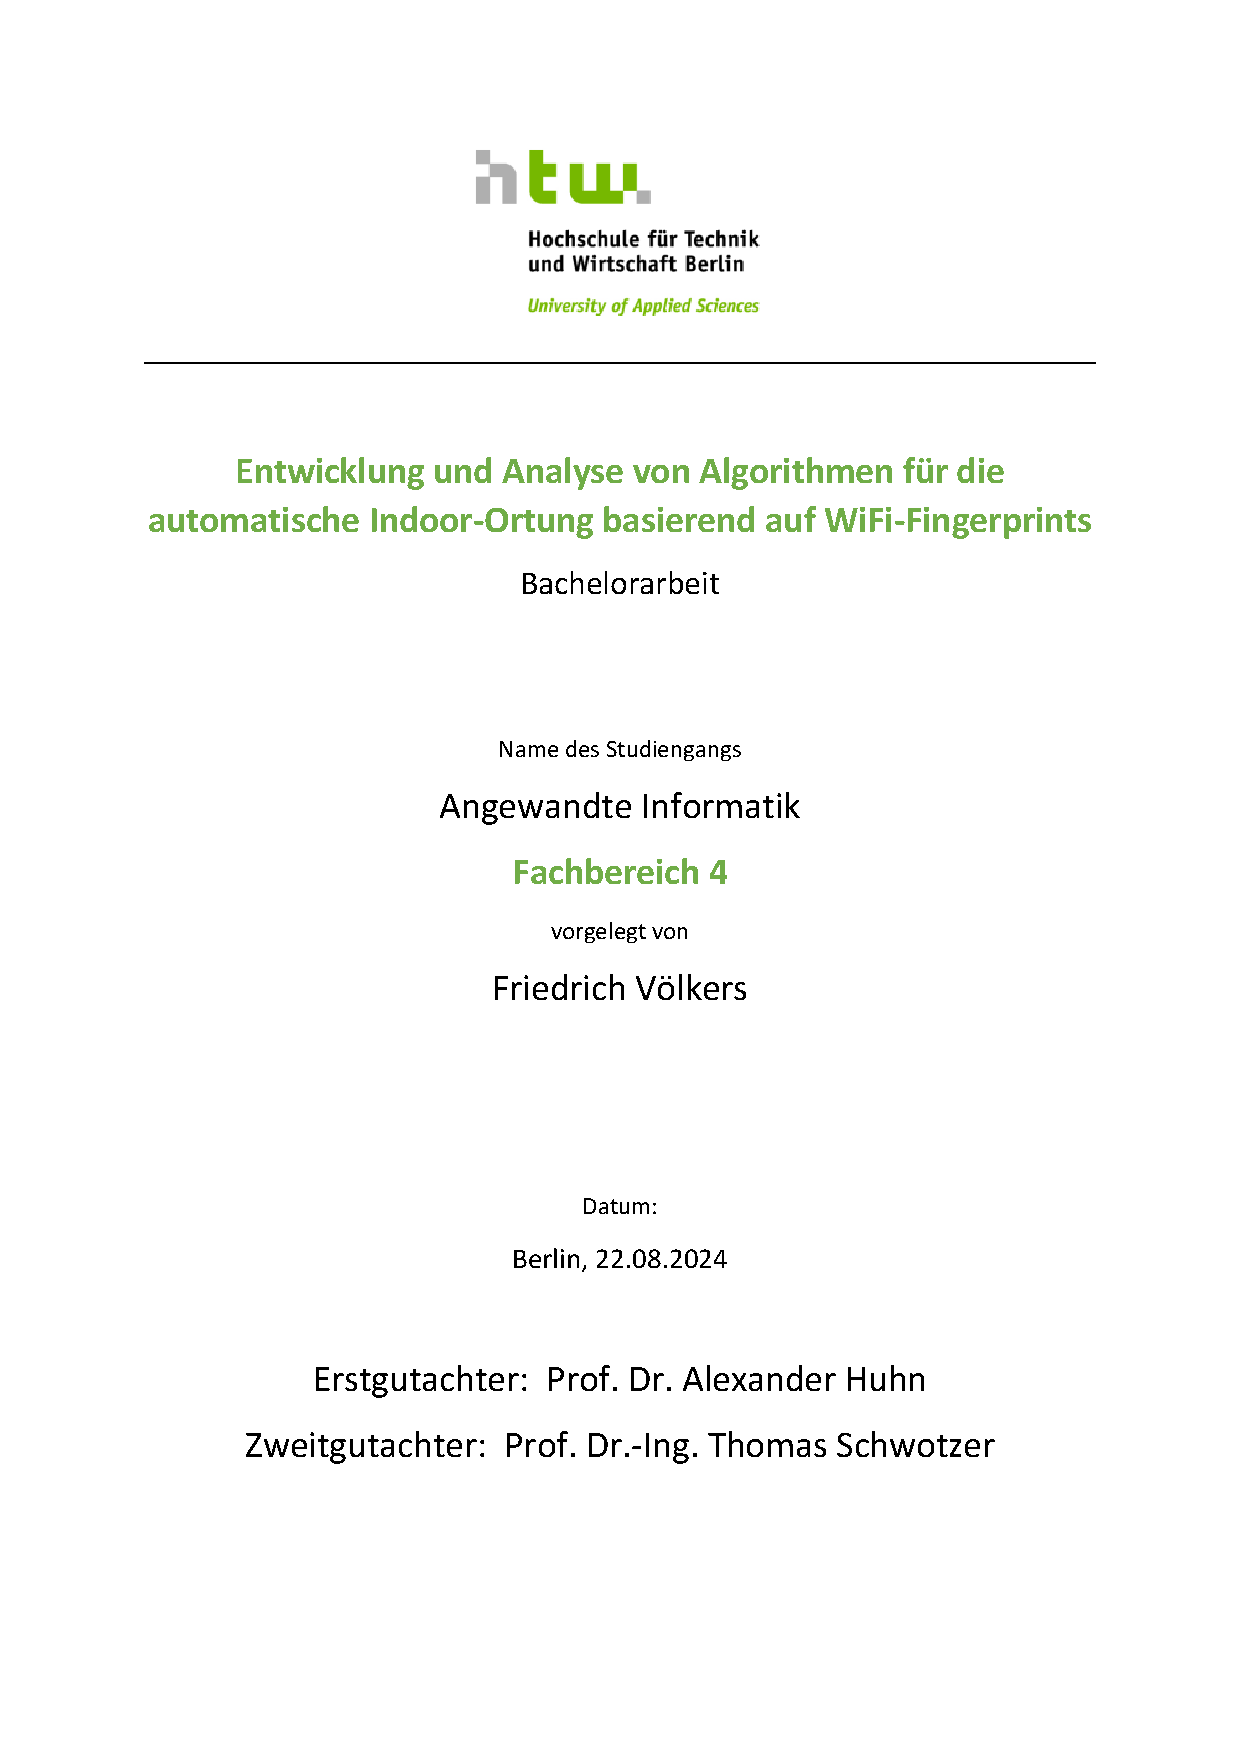
\includepdf[pages=1]{deckblatt.pdf}


% Title page without numbering
\pagenumbering{gobble}

% Title page
% \begin{titlepage}
%     \centering
%     \includegraphics[width=0.3\textwidth]{htw_logo.jpg}\par
%     \vspace*{1.6cm}
%     {\Huge\bfseries Entwicklung und Analyse von Algorithmen für die automatische Indoor-Ortung basierend auf WiFi-Fingerprints \par}
%     \vspace{1.5cm}
%     {\LARGE Bachelorarbeit \par}
%     \vspace{2cm}
%     {\Large\itshape Friedrich Völkers \par}
%     {\itshape 585012 \par}
%     \vfill
%     Betreuer: Prof. Dr. Alexander Huhn \\
%     Zweitbetreuer: Prof. Dr.-Ing. Thomas Schwotzer
%     \vspace{1cm}
%     \vfill
%     {\large \today\par}
% \end{titlepage}

% Directories with Roman numbering
\pagenumbering{Roman}

% Table of contents without numbering
\tableofcontents

% Verzeichnis der Listings
% \listofcodes

\begingroup
\setlength{\parskip}{1em} % Adjust the spacing for the list of listings
\lstlistoflistings
\endgroup


% List of figures without numbering
\listoffigures

% List of tables without numbering
\listoftables

% Main content with Arabic numbering
\clearpage
\pagenumbering{arabic}

% Including chapters




% \chapter{Einleitung}

In der vorliegenden Arbeit werden verschiedene Algorithmen zur Indoor-Ortung basierend auf WiFi-Fingerprints analysiert und implementiert. Dafür werden diese Algorithmen ausführlich in Kapitel \ref{algorithmen} beschrieben, in Kapitel \ref{implementierung} implementiert und in den Kapitel \ref{untersuchungen}, \ref{datenaufbereitung} und \ref{erweiterte_untersuchungen} mit der in Kapitel \ref{testanwendung} beschriebenen Testanwendung analysiert und verglichen. Grundlage der Untersuchungen sind Datensätze, welche in Kapitel \ref{datenerhebung} erfasst wurden. Das Ziel dieser Arbeit ist es, die Genauigkeit der verschiedenen Algorithmen zu untersuchen und zu ermitteln unter welchen Bedingungen und mit welchem Algorithmus in den meisten Fällen eine korrekte Ortung möglich ist. 

Die Ergebnisse dieser Arbeit sollen als Grundlage für die automatischen Indoor-Ortung in der HTW Berlin dienen, sodass zum Beispiel Microcontroller wie der \textit{ESP32} autonom den Raum erkennen können, in dem sie sich befinden. Des Weiteren wird die App \textit{BVG Detection} wieder in Betrieb genommen und dazu verwendet WiFi-Fingerprints zu erfassen und die Position des Nutzers zu bestimmen.

Der verwendete Quellcode ist auf der \textit{GitLab}-Instanz der HTW Berlin unter \url{https://gitlab.rz.htw-berlin.de/s0585012/wifi-fingerprint-based-indoor-localization} gespeichert.

% \chapter{Grundlagen}
% Der \gls{accesspoint} sendet die \gls{bssid} und die \gls{ssid}, damit Geräte, wie eine \gls{vm}, sich verbinden können. Algorithmen wie \gls{knn} und \gls{svm} können in einer \gls{api} implementiert werden, um die Datenverarbeitung zu optimieren.


% Quelle 1: Access Points Service Set Identifier (SSID) for Localization and Tracking -> masoud2022access
% Quelle 2: RSSI-Based Indoor Localization With the Internet of Things -> sadowski2018rssi
% Quelle 3: Survey on Indoor localization System and Recent Advances of WIFI Fingerprinting Technique -> basri2016survey

% Das ist eine Test Zitierung\myfootcite{TORRESSOSPEDRA20159263}{S. 23}.

\section{Indoor-Ortung via WiFi Fingerprints}

WiFi-Fingerprinting ist eine Technik die zur Lokalisierung in Innenräumen verwendet werden kann. Dabei werden an verschiedenen Positionen in einem Gebäude die Signalstärken der empfangenden WLAN-Router - die sogenannten Access Points - gemessen und in einer Datenbank gespeichert. Dadurch dass an verschiedenen Positionen verschiedene Access Points unterschiedlich stark empfangen werden, entsteht eine Art Fingerabdruck dieser Position, welcher verwendet werden kann um die Position eines Geräts anhand der empfangenen Access Points und deren Signalstärke zu bestimmen.

Das Prinzip der WiFi-Fingerprinting-basierten Ortung kann in eine Offline- und eine Online-Phase unterteilt werden. In der Offline-Phase werden die Fingerprints aufgezeichnet und mit den dazugehörigen Positionen gespeichert. In der Online-Phase wird die aktuelle Position eines Geräts bestimmt, indem dieses ebenfalls einen WiFi-Fingerprint aufzeichnet und diesen mit den bekannten Fingerprints in der Datenbank abgleicht. Die Position des Geräts wird anschließend anhand des am besten passenden Fingerprints bestimmt. 

Neben der Indoor-Ortung mittels WiFi-Fingerprinting können auch andere Technologien wie Bluetooth, Ultra-wideband, RFID und Zigbee verwendet werden, wobei jede Technik seine Vor- und Nachteile mit sich bringt. Die Vorteile des WiFi-Fingerprinting sind, dass diese in vielen Fällen verwendet werden kann ohne zusätzliche Hardware zu installieren, da die meisten Gebäude bereits über eine WLAN-Infrastruktur verfügen. Zudem ist die Reichweite von WLAN-Signalen größer als die von Bluetooth oder RFID, wodurch insgesamt weniger Hardware benötigt wird. Der Nachteil dieser Technik ist jedoch der zeitliche Aufwand beim Erstellen der Fingerprints während der Offline-Phase\myfootcite{Shang2022WiFiFingerprinting}{S. 726 ff.}.

\section{Technische Grundlagen}

Ein WiFi-Fingerprint kann definiert werden als eine Liste der empfangenen Access Points, wobei in jedem Eintrag die MAC-Adresse und die Signalstärke steht.\myfootcite{Shang2022WiFiFingerprinting}{S. 729} In dieser Arbeit wurden diese Einträge um die Klarnamen der Netzwerke - die so genannte SSID - erweitert.

\subsection{BSSID}

Der Basic Service Set Identifier (BSSID) ist die eindeutige Kennung eines Access Points und entspricht der MAC-Adresse des Access Points. Diese Adresse ist unveränderlich und kann dazu verwendet werden  einen Access Point eindeutig zu identifizieren.\myfootcite{Amirisoori2017}{S. 27}

\subsection{SSID}

Der Service Set Identifier (SSID) ist ein eindeutiger Bezeichner, der ein drahtloses Netzwerk kennzeichnet und aus einer alphanumerische Zeichenfolgen - wie zum Beispiel \textit{eduroam} oder \textit{FRITZ!Box 7590 XY} - besteht. Im Gegensatz zur BSSID kann die SSID frei gewählt werden, wodurch mehrere Access Points die selbe SSID haben können.\myfootcite{masoud2022access}{S. 5460} % (Quelle 1, Kapitel 1, Seite 5460).

\subsection{RSSI} \label{rssi}

Der Received Signal Strength Indicator (RSSI) ist ein relativer Indikator für die Empfangsstärke eines kabellosen Kommunikationssystems nach IEEE 802.11 Standard und gibt die Qualität eines empfangen Signals auf einer Skale von -100 bis 0 in der Einheit dBm an. Je größer der Wert ist, also je näher dieser an 0 ist, desto besser ist das Signal.\mycitefoot{iotmeshRSSIReceived}

\section{Zusammenhang zwischen Signalstärke und Distanz} \label{pfadverlustmodell}

Da für Indoor-Ortung mittels WiFi-Fingerprints die RSSI-Werte der Access Points verwendet werden, ist es hilfreich den Zusammenhang zwischen der Signalstärke un der Entfernung zu verstehen. Die RSSI-Werte sind abhängig von der Entfernung zwischen dem Sender und dem Empfänger und nehmen mit zunehmender Distanz ab. Der Zusammenhang zwischen dem RSSI-Wert und der Entfernung kann durch das Pfadverlustmodell (siehe Gleichung \ref{eq:rssi}) beschrieben werden.

\begin{equation}
    RSSI = -10 * n * \log_{10}(d) + C
    \label{eq:rssi}
\end{equation}

Dabei ist \(n\) der Pfadverlustexponent, der je nach Umgebung variiert, \(d\) die Distanz zwischen Sender und Empfänger und \(C\) eine Konstante, die die Systemverluste berücksichtigt.\myfootcite{sadowski2018rssi}{S. 30153}

In dem Paper \textit{RSSI-Based Indoor Localization With the Internet of Things} wurden die Parameter des Pfadverlustmodells experimentell in einer Umgebung untersucht, welche mit der in dieser Arbeit verwendeten vergleichbar ist.\mycitefoot{sadowski2018rssi} Die Experimente wurden in einem Forschungslabor (10,8 m x 7,3 m) - welches mit mehreren WiFi- und Bluetooth-Geräten und Computern ausgestattet ist - durchgeführt. In dieser Umgebung ergaben die Untersuchungen einen Pfadverlustexponenten von \(n = 2.013\) und eine Konstante von \(C = -49.99\) dBm.\myfootcite{sadowski2018rssi}{S. 30157}

Das Pfadverlustmodell mit den Ergebnissen aus der erwähnten Studie ist in Abbildung \ref{fig:plot_rssi_distance} dargestellt und dient als Grundlage für die in Kapitel \ref{datenaufbereitung} untersuchten Datenaufbereitungsschritte.

\begin{figure}[H]
    \centering
    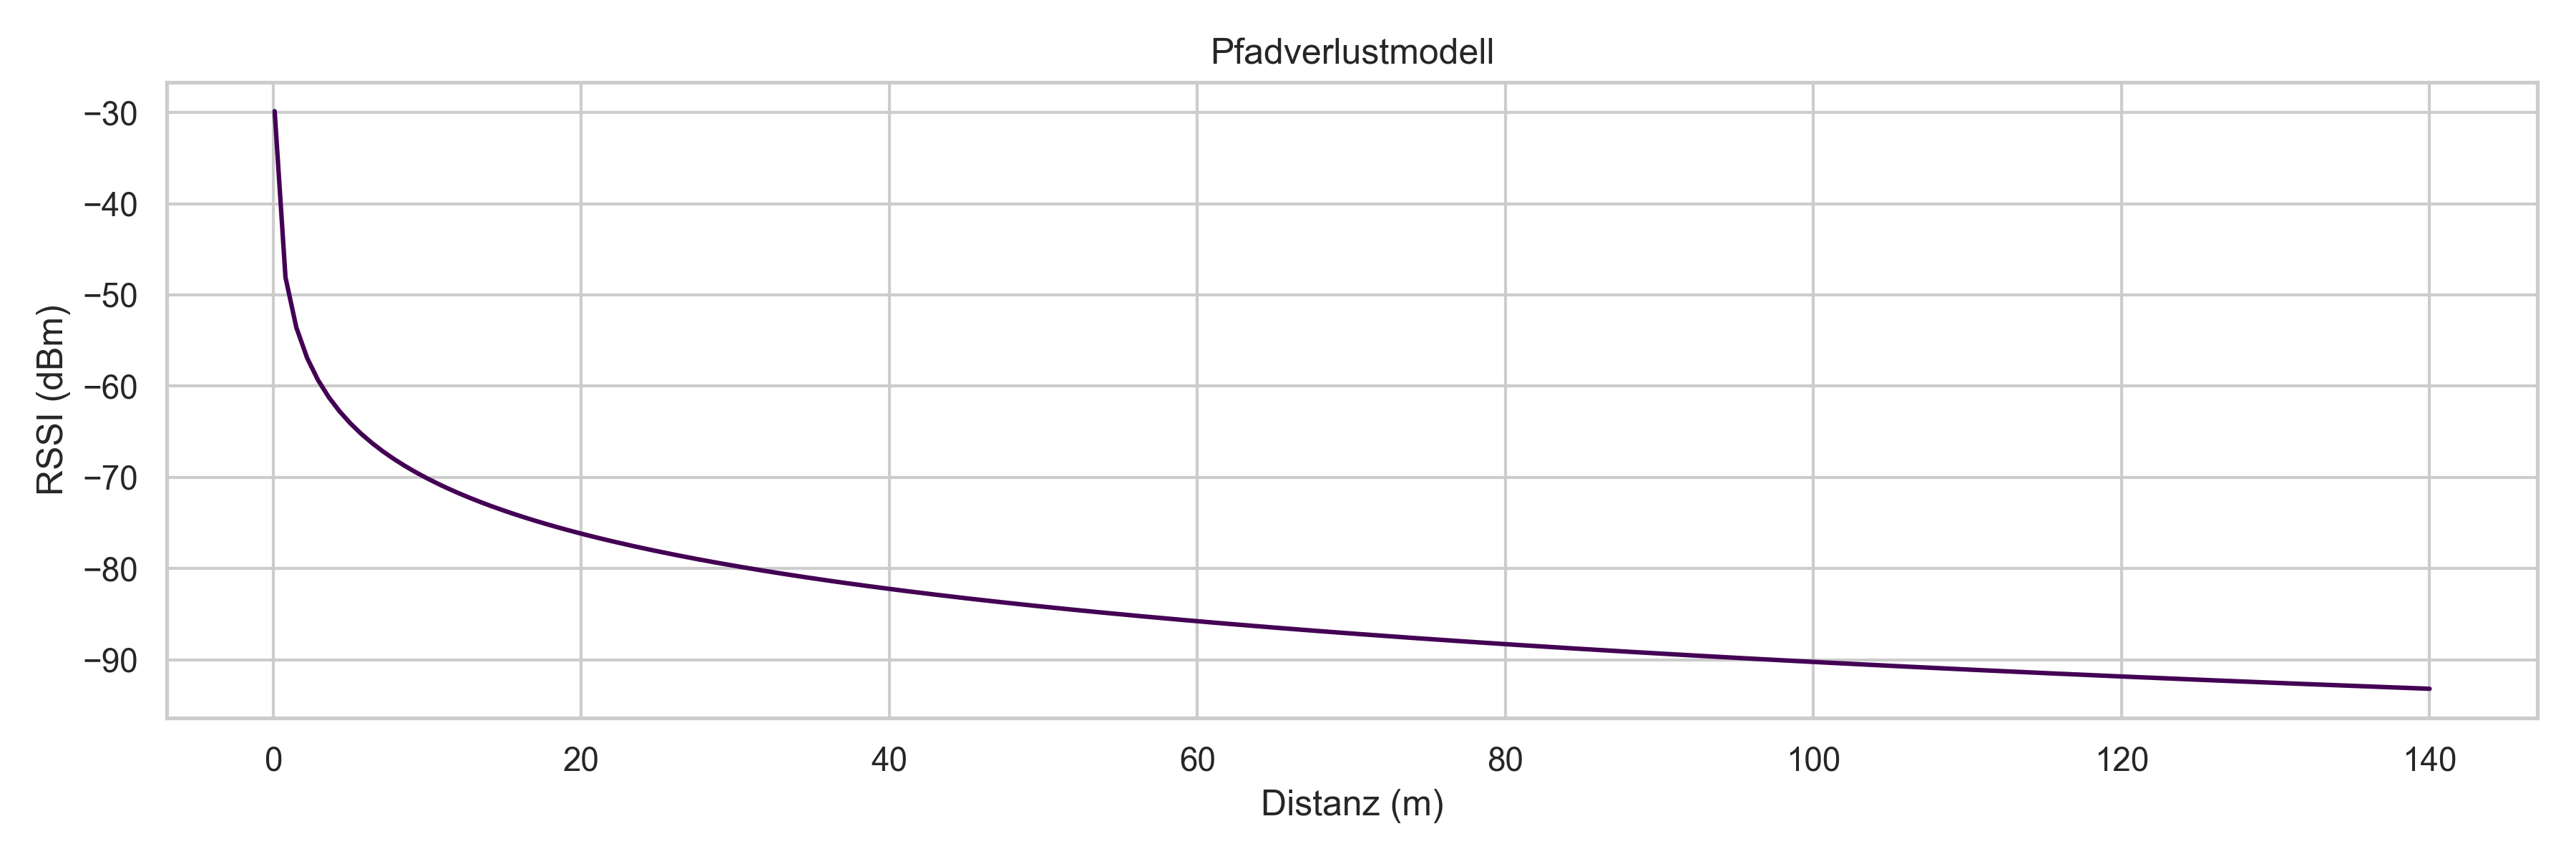
\includegraphics[width=0.8\textwidth]{images/plot_rssi_distance.png}
    \caption{Exemplarischer Zusammenhang zwischen RSSI-Werten und der Entfernung nach dem Pfadverlustmodell}
    \label{fig:plot_rssi_distance}
\end{figure}
% \input{chapters/03_systemarchitektur}
% \input{chapters/04_implementierungsdetails}
% \input{chapters/05_datenerfassung_aufbereitung}
% \input{chapters/06_vergleich_algorithmen}
% \input{chapters/07_erweiterte_untersuchungen}
% \input{chapters/08_ergebnisse_diskussion}
% \input{chapters/09_fazit_ausblick}

\chapter{Einleitung}

In der vorliegenden Arbeit werden verschiedene Algorithmen zur Indoor-Ortung basierend auf WiFi-Fingerprints analysiert und implementiert. Dafür werden diese Algorithmen ausführlich in Kapitel \ref{algorithmen} beschrieben, in Kapitel \ref{implementierung} implementiert und in den Kapitel \ref{untersuchungen}, \ref{datenaufbereitung} und \ref{erweiterte_untersuchungen} mit der in Kapitel \ref{testanwendung} beschriebenen Testanwendung analysiert und verglichen. Grundlage der Untersuchungen sind Datensätze, welche in Kapitel \ref{datenerhebung} erfasst wurden. Das Ziel dieser Arbeit ist es, die Genauigkeit der verschiedenen Algorithmen zu untersuchen und zu ermitteln unter welchen Bedingungen und mit welchem Algorithmus in den meisten Fällen eine korrekte Ortung möglich ist. 

Die Ergebnisse dieser Arbeit sollen als Grundlage für die automatischen Indoor-Ortung in der HTW Berlin dienen, sodass zum Beispiel Microcontroller wie der \textit{ESP32} autonom den Raum erkennen können, in dem sie sich befinden. Des Weiteren wird die App \textit{BVG Detection} wieder in Betrieb genommen und dazu verwendet WiFi-Fingerprints zu erfassen und die Position des Nutzers zu bestimmen.

Der verwendete Quellcode ist auf der \textit{GitLab}-Instanz der HTW Berlin unter \url{https://gitlab.rz.htw-berlin.de/s0585012/wifi-fingerprint-based-indoor-localization} gespeichert.

\chapter{Grundlagen}
% Der \gls{accesspoint} sendet die \gls{bssid} und die \gls{ssid}, damit Geräte, wie eine \gls{vm}, sich verbinden können. Algorithmen wie \gls{knn} und \gls{svm} können in einer \gls{api} implementiert werden, um die Datenverarbeitung zu optimieren.


% Quelle 1: Access Points Service Set Identifier (SSID) for Localization and Tracking -> masoud2022access
% Quelle 2: RSSI-Based Indoor Localization With the Internet of Things -> sadowski2018rssi
% Quelle 3: Survey on Indoor localization System and Recent Advances of WIFI Fingerprinting Technique -> basri2016survey

% Das ist eine Test Zitierung\myfootcite{TORRESSOSPEDRA20159263}{S. 23}.

\section{Indoor-Ortung via WiFi Fingerprints}

WiFi-Fingerprinting ist eine Technik die zur Lokalisierung in Innenräumen verwendet werden kann. Dabei werden an verschiedenen Positionen in einem Gebäude die Signalstärken der empfangenden WLAN-Router - die sogenannten Access Points - gemessen und in einer Datenbank gespeichert. Dadurch dass an verschiedenen Positionen verschiedene Access Points unterschiedlich stark empfangen werden, entsteht eine Art Fingerabdruck dieser Position, welcher verwendet werden kann um die Position eines Geräts anhand der empfangenen Access Points und deren Signalstärke zu bestimmen.

Das Prinzip der WiFi-Fingerprinting-basierten Ortung kann in eine Offline- und eine Online-Phase unterteilt werden. In der Offline-Phase werden die Fingerprints aufgezeichnet und mit den dazugehörigen Positionen gespeichert. In der Online-Phase wird die aktuelle Position eines Geräts bestimmt, indem dieses ebenfalls einen WiFi-Fingerprint aufzeichnet und diesen mit den bekannten Fingerprints in der Datenbank abgleicht. Die Position des Geräts wird anschließend anhand des am besten passenden Fingerprints bestimmt. 

Neben der Indoor-Ortung mittels WiFi-Fingerprinting können auch andere Technologien wie Bluetooth, Ultra-wideband, RFID und Zigbee verwendet werden, wobei jede Technik seine Vor- und Nachteile mit sich bringt. Die Vorteile des WiFi-Fingerprinting sind, dass diese in vielen Fällen verwendet werden kann ohne zusätzliche Hardware zu installieren, da die meisten Gebäude bereits über eine WLAN-Infrastruktur verfügen. Zudem ist die Reichweite von WLAN-Signalen größer als die von Bluetooth oder RFID, wodurch insgesamt weniger Hardware benötigt wird. Der Nachteil dieser Technik ist jedoch der zeitliche Aufwand beim Erstellen der Fingerprints während der Offline-Phase\myfootcite{Shang2022WiFiFingerprinting}{S. 726 ff.}.

\section{Technische Grundlagen}

Ein WiFi-Fingerprint kann definiert werden als eine Liste der empfangenen Access Points, wobei in jedem Eintrag die MAC-Adresse und die Signalstärke steht.\myfootcite{Shang2022WiFiFingerprinting}{S. 729} In dieser Arbeit wurden diese Einträge um die Klarnamen der Netzwerke - die so genannte SSID - erweitert.

\subsection{BSSID}

Der Basic Service Set Identifier (BSSID) ist die eindeutige Kennung eines Access Points und entspricht der MAC-Adresse des Access Points. Diese Adresse ist unveränderlich und kann dazu verwendet werden  einen Access Point eindeutig zu identifizieren.\myfootcite{Amirisoori2017}{S. 27}

\subsection{SSID}

Der Service Set Identifier (SSID) ist ein eindeutiger Bezeichner, der ein drahtloses Netzwerk kennzeichnet und aus einer alphanumerische Zeichenfolgen - wie zum Beispiel \textit{eduroam} oder \textit{FRITZ!Box 7590 XY} - besteht. Im Gegensatz zur BSSID kann die SSID frei gewählt werden, wodurch mehrere Access Points die selbe SSID haben können.\myfootcite{masoud2022access}{S. 5460} % (Quelle 1, Kapitel 1, Seite 5460).

\subsection{RSSI} \label{rssi}

Der Received Signal Strength Indicator (RSSI) ist ein relativer Indikator für die Empfangsstärke eines kabellosen Kommunikationssystems nach IEEE 802.11 Standard und gibt die Qualität eines empfangen Signals auf einer Skale von -100 bis 0 in der Einheit dBm an. Je größer der Wert ist, also je näher dieser an 0 ist, desto besser ist das Signal.\mycitefoot{iotmeshRSSIReceived}

\section{Zusammenhang zwischen Signalstärke und Distanz} \label{pfadverlustmodell}

Da für Indoor-Ortung mittels WiFi-Fingerprints die RSSI-Werte der Access Points verwendet werden, ist es hilfreich den Zusammenhang zwischen der Signalstärke un der Entfernung zu verstehen. Die RSSI-Werte sind abhängig von der Entfernung zwischen dem Sender und dem Empfänger und nehmen mit zunehmender Distanz ab. Der Zusammenhang zwischen dem RSSI-Wert und der Entfernung kann durch das Pfadverlustmodell (siehe Gleichung \ref{eq:rssi}) beschrieben werden.

\begin{equation}
    RSSI = -10 * n * \log_{10}(d) + C
    \label{eq:rssi}
\end{equation}

Dabei ist \(n\) der Pfadverlustexponent, der je nach Umgebung variiert, \(d\) die Distanz zwischen Sender und Empfänger und \(C\) eine Konstante, die die Systemverluste berücksichtigt.\myfootcite{sadowski2018rssi}{S. 30153}

In dem Paper \textit{RSSI-Based Indoor Localization With the Internet of Things} wurden die Parameter des Pfadverlustmodells experimentell in einer Umgebung untersucht, welche mit der in dieser Arbeit verwendeten vergleichbar ist.\mycitefoot{sadowski2018rssi} Die Experimente wurden in einem Forschungslabor (10,8 m x 7,3 m) - welches mit mehreren WiFi- und Bluetooth-Geräten und Computern ausgestattet ist - durchgeführt. In dieser Umgebung ergaben die Untersuchungen einen Pfadverlustexponenten von \(n = 2.013\) und eine Konstante von \(C = -49.99\) dBm.\myfootcite{sadowski2018rssi}{S. 30157}

Das Pfadverlustmodell mit den Ergebnissen aus der erwähnten Studie ist in Abbildung \ref{fig:plot_rssi_distance} dargestellt und dient als Grundlage für die in Kapitel \ref{datenaufbereitung} untersuchten Datenaufbereitungsschritte.

\begin{figure}[H]
    \centering
    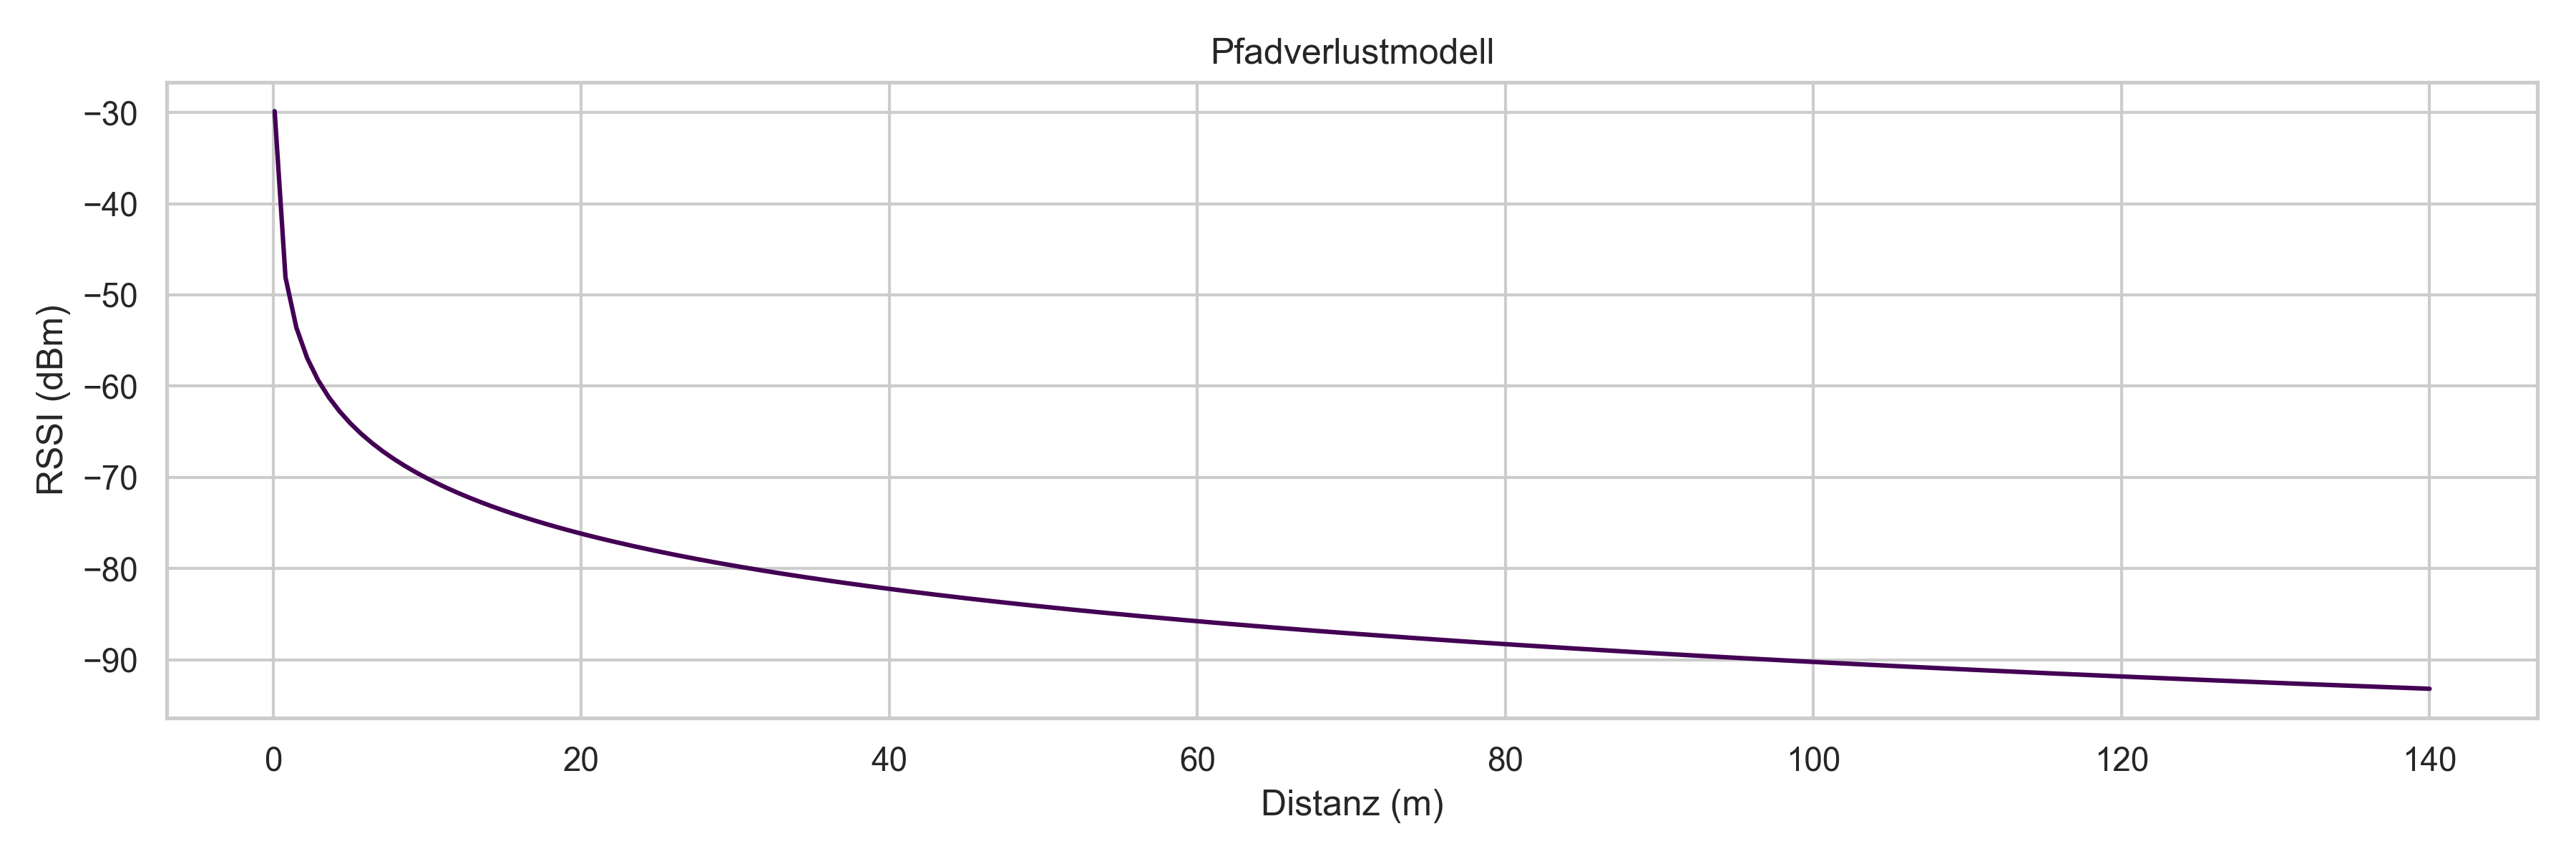
\includegraphics[width=0.8\textwidth]{images/plot_rssi_distance.png}
    \caption{Exemplarischer Zusammenhang zwischen RSSI-Werten und der Entfernung nach dem Pfadverlustmodell}
    \label{fig:plot_rssi_distance}
\end{figure}
\chapter{Algorithmen} \label{algorithmen}

% Beispiel für Glossar/Abkürzungen
% Der \gls{accesspoint} sendet die \gls{bssid} und die \gls{ssid}, damit Geräte, wie eine \gls{vm}, sich verbinden können. Algorithmen wie \gls{knn} und \gls{svm} können in einer \gls{api} implementiert werden, um die Datenverarbeitung zu optimieren.


% \begin{table}[h]
%     \centering
%     \begin{tabularx}{\textwidth}{|X|X|X|X|X|}
%         \hline
%         Router & Raum 1      & Raum 2      & Raum 3     & Unbekannt (1) \\ \hline
%         1      & -73.67 dBm  & -91.12 dBm  & -69.37 dBm & -73.51 dBm    \\ \hline
%         2      & -104.99 dBm & -64.47 dBm  & -89.65 dBm & -103.41 dBm   \\ \hline
%         3      & -67.03 dBm  & -105.38 dBm & -88.40 dBm & -70.35 dBm    \\ \hline
%     \end{tabularx}
%     \caption{RSSI-Werte für die drei Router und die Räume}
%     \label{tab:rssi_values}
% \end{table}

Für die Vorhersage einer Position bei der Indoor-Ortung mittels WiFi-Fingerprints können verschiedene Algorithmen verwendet werden. Es wurde sich dafür entschieden in dieser Arbeit die Modelle K-Nearest Neighbors (KNN), Support Vector Machines (SVM) und Random Forest zu verwenden, da diese Modelle bereits in anderen Untersuchungen gute Ergebnisse erzielen konnten.\myfootcite{Han2018WirelessFingerprint}{S. 3}\textsuperscript{,}\myfootcite{Rezgui2017NormalizedSVM}{S. 13}

Im Folgenden werden die drei verwendeten Algorithmen detailliert beschrieben und für eine bessere Verständlichkeit anhand eines Beispiels, welches in Tabelle \ref{tab:trainingsdaten} dargestellt ist, erläutert. In diesem Beispiel wurden die RSSI-Werte von sechs Messungen in drei verschiedenen Räumen sowie drei Access Points simuliert. In der Tabelle \ref{tab:testdaten} sind die RSSI-Werte von einer Messung in einem unbekannten Raum, für die eine Vorhersage gemacht werden soll, aufgeführt. Die in den Tabellen dargestellten Werte basieren nicht auf realen Messungen und sind hypothetische Beispielwerte, welche gewählt wurden, um die Funktionsweise der Algorithmen zu veranschaulichen und die Nachvollziehbarkeit der Berechnungen zu erleichtern.

\begin{table}[h]
    \centering
    \begin{tabularx}{\textwidth}{|X|X|X|X|X|}
        \hline
        Messung & Raum & AP1 & AP2 & AP3 \\ \hline
        1 & A & -45 dBm & -60 dBm & -70 dBm \\ \hline
        2 & A & -46 dBm & -61 dBm & -71 dBm \\ \hline
        3 & B & -55 dBm & -65 dBm & -75 dBm \\ \hline
        4 & B & -54 dBm & -66 dBm & -74 dBm \\ \hline
        5 & C & -50 dBm & -70 dBm & -80 dBm \\ \hline
        6 & C & -51 dBm & -69 dBm & -79 dBm \\ \hline
    \end{tabularx}
    \caption{Beispielwerte von WiFi-Fingerprints aus der Offline-Phase}
    \label{tab:trainingsdaten}
\end{table}

\begin{table}[h]
    \centering
    \begin{tabularx}{\textwidth}{|X|X|X|X|X|}
        \hline
        Messung & Raum & AP1 & AP2 & AP3 \\ \hline
        - & - & -52 dBm & -68 dBm & -78 dBm \\ \hline
    \end{tabularx}
    \caption{Beispielwerte eines WiFi-Fingerprints aus der Online-Phase}
    \label{tab:testdaten}
\end{table}


% \mycitefoot{Shang2022WiFiFingerprinting}
% \myfootcite{masoud2022access}{S. 5464}

% \paragraph{Quellen für Auswahl}

% \begin{itemize}
%     \item https://ar5iv.labs.arxiv.org/html/2111.14281 -> KNN, SVM % Hoang2021PassiveLocalization
%     \item A Wireless Fingerprint Location Method Based on Target Tracking (Kapitel 3, Seite 3) -> KNN, SVM, Random Forest % Han2018WirelessFingerprint
%     \item https://onlinelibrary.wiley.com/doi/full/10.1155/2017/6268797 Name: An Efficient Normalized Rank Based SVM for Room Level Indoor WiFi Localization with Diverse Devices -> KNN, SVM, Random Forest. In Table 2 stehen die Genauigkeiten der Algorithmen S. 13% Rezgui2017NormalizedSVM
% \end{itemize}

\section{K-Nearest Neighbors (KNN)}

% \textbf{Quellen:} \\
% \href{https://www.ibm.com/de-de/topics/knn}{Quelle 1: https://www.ibm.com/de-de/topics/knn} \\ % ibmknearestNeighbors
% Quelle 4: Comprehensive analysis of distance and similarity measures for Wi-Fi fingerprinting indoor positioning systems \\ % TorresSospedra2015WiFi
% Quelle 5: Hechenbichler, Schliep: - Weighted k-Nearest-Neighbor Techniques and Ordinal Classification % Hechenbichler2004WeightedKNN

% \subsection{Algorithmusbeschreibung}

Der \gls{knn} Algorithmus ist ein überwachter Lernalgorithmus, der auf dem Konzept der Nähe basiert und zur Lösung von Klassifikations- und Regressionsproblemen verwendet werden kann. Der Algorithmus funktioniert so, dass ein Datenpunkt mit den vorhandenen Datenpunkten in den Trainingsdaten verglichen wird und die Distanz zu jedem Datenpunkt berechnet wird. Dabei wird die Distanz der einzelnen Features, welche in dem Fall der Indoor-Ortung die RSSI-Werte der Access Points sind, berechnet und aufsummiert. Basierend auf diesen Distanzen werden die \( k \)-Datenpunkte ausgewählt, die den kleinsten Abstand haben. Aus diesen \( k \)-Datenpunkten wird dann die Klasse vorhergesagt, die am häufigsten vertreten ist. Bei der Indoor-Ortung entsprechen die Klassen den verschiedenen Räumen.\mycitefoot{ibmknearestNeighbors}

\subsection{Distanzmetriken}
Für die Berechnung der Distanzen können verschiedene Distanzmetriken verwendet werden. Die am häufigsten verwendete Distanzmetrik ist der euklidische Abstand. Bei der euklidischen Distanz wird das Quadrat der Abstände zwischen zwei Werten gebildet, über alle Wertepaare aufsummiert und abschließend die Quadratwurzel dieser Summe gezogen (siehe Gleichung \ref{eq:euclidean}).\mycitefoot{ibmknearestNeighbors}

\begin{equation}
    \label{eq:euclidean}
    \text{distance}_{\text{euclidean}}(P, Q) = \sqrt{\sum_{i=1}^{d} (P_i - Q_i)^2}
\end{equation}

Bei der Sørensen-Distanzfunktion werden die Beträge der Abstände der Datenpunkte aufsummiert und durch die Summe der addierten Wertepaare geteilt (siehe Gleichung \ref{eq:sorensen}). Grund für die Wahl dieser beiden Metriken sind die Ergebnisse der Arbeit \textit{Comprehensive analysis of distance and similarity measures for Wi-Fi fingerprinting indoor positioning systems}, welche mit der Sørensen Distanz gute Ergebnisse erzielen konnte und die Tatsache, dass die euklidische Distanz weit verbreitet ist und der bisherigen Implementierung in der \textit{BVG Detection} App entspricht.\mycitefoot{TorresSospedra2015WiFi}

\begin{equation}
    \label{eq:sorensen}
    \text{distance}_{\text{sorensen}}(P, Q) = \frac{\sum_{i=1}^{d} |P_i - Q_i|}{\sum_{i=1}^{d} (P_i + Q_i)}
\end{equation}

Um die Unterschiede dieser beiden Metriken zu veranschaulichen, wurden die Distanzen für alle möglichen Wertepaare zwischen 0\,dBm und -100\,dBm berechnet und in Abbildung \ref{fig:distance_metrics_heatmaps} dargestellt. Wie zu erkennen ist, ist bei der euklidischen Distanz ausschließlich die Differenz der beiden Werte ausschlaggebend, was sich anhand der symmetrischen Anordnung der Werte in der Heatmap entlang der Geraden, die durch die Punkte (0\,dBm, -100\,dBm) und (-100\,dBm, 0\,dBm) sowie (0\,dBm, 0\,dBm) und (-100\,dBm, -100\,dBm) verläuft, zeigt. Im Gegensatz dazu ist die Sørensen-Distanz sowohl von der Differenz als auch von der Summe der beiden Werte abhängig, was sich durch das Fehlen einer Symmetrie entlang der genannten Geraden zwischen den Punkten (0\,dBm, -100\,dBm) und (-100\,dBm, 0\,dBm) zeigt. Bei kleineren Werten ist ein größerer Abstand erforderlich, um die gleiche Distanz wie bei größeren Werten zu erreichen. Dies könnte sich vorteilhaft auf die Indoor-Ortung auswirken, da die RSSI-Werte nicht linear mit der Entfernung korrelieren, wie in Abbildung \ref{fig:plot_rssi_distance} dargestellt ist.


% Um dies zu verdeutlichen, betrachten wir die Berechnung der Distanzen für zwei Beispielwertepaare:

% Gegeben:
% \begin{itemize}
%     \item Wertepaar 1: \( P = -30 \, \text{dBm} \), \( Q = -40 \, \text{dBm} \)
%     \item Wertepaar 2: \( P = -70 \, \text{dBm} \), \( Q = -80 \, \text{dBm} \)
% \end{itemize}

% \begin{table}[H]
%     \centering
%     \begin{tabular}{|c|c|c|}
%         \hline
%         Wertepaar                                & Sørensen-Dice Distanz & Euklidische Distanz \\
%         \hline
%         \(-30 \, \text{dBm}, -40 \, \text{dBm}\) & \(-0.142857\)         & \(10\)              \\
%         \(-70 \, \text{dBm}, -80 \, \text{dBm}\) & \(-0.066667\)         & \(10\)              \\
%         \hline
%     \end{tabular}
%     \caption{Berechnete Distanzen für die gegebenen Wertepaare}
%     \label{tab:distance_results}
% \end{table}

% Um das zu verdeutlichen wurden die Distanzen für beide Metriken anhand der Beispielwerte berechnet wie in Tabelle \ref{tab:distanzen} dargestellt.

Für die Beispielwerte ergeben sich dadurch folgende Distanzen

Die sich für die Beispielwerte aus Tabelle \ref{tab:trainingsdaten} ergebenen Distanzen sind in Tabelle \ref{tab:distanzen} dargestellt.

\begin{table}[h]
    \centering
    \begin{tabularx}{\textwidth}{|X|X|X|X|}
        \hline
        Messung & Raum & Euklidische Distanz & Sørensen Distanz \\ \hline
        1 & A & 11.0 & 0.084 \\ \hline
        2 & A & 9.8 & 0.077 \\ \hline
        3 & B & 5.2 & 0.034 \\ \hline
        4 & B & 4.5 & 0.030 \\ \hline
        5 & C & 3.5 & 0.020 \\ \hline
        6 & C & 2.6 & 0.015 \\ \hline
    \end{tabularx}
    \caption{Berechnete Distanzen der Beispieldaten}
    \label{tab:distanzen}
\end{table}

\begin{figure}[H]
    \centering
    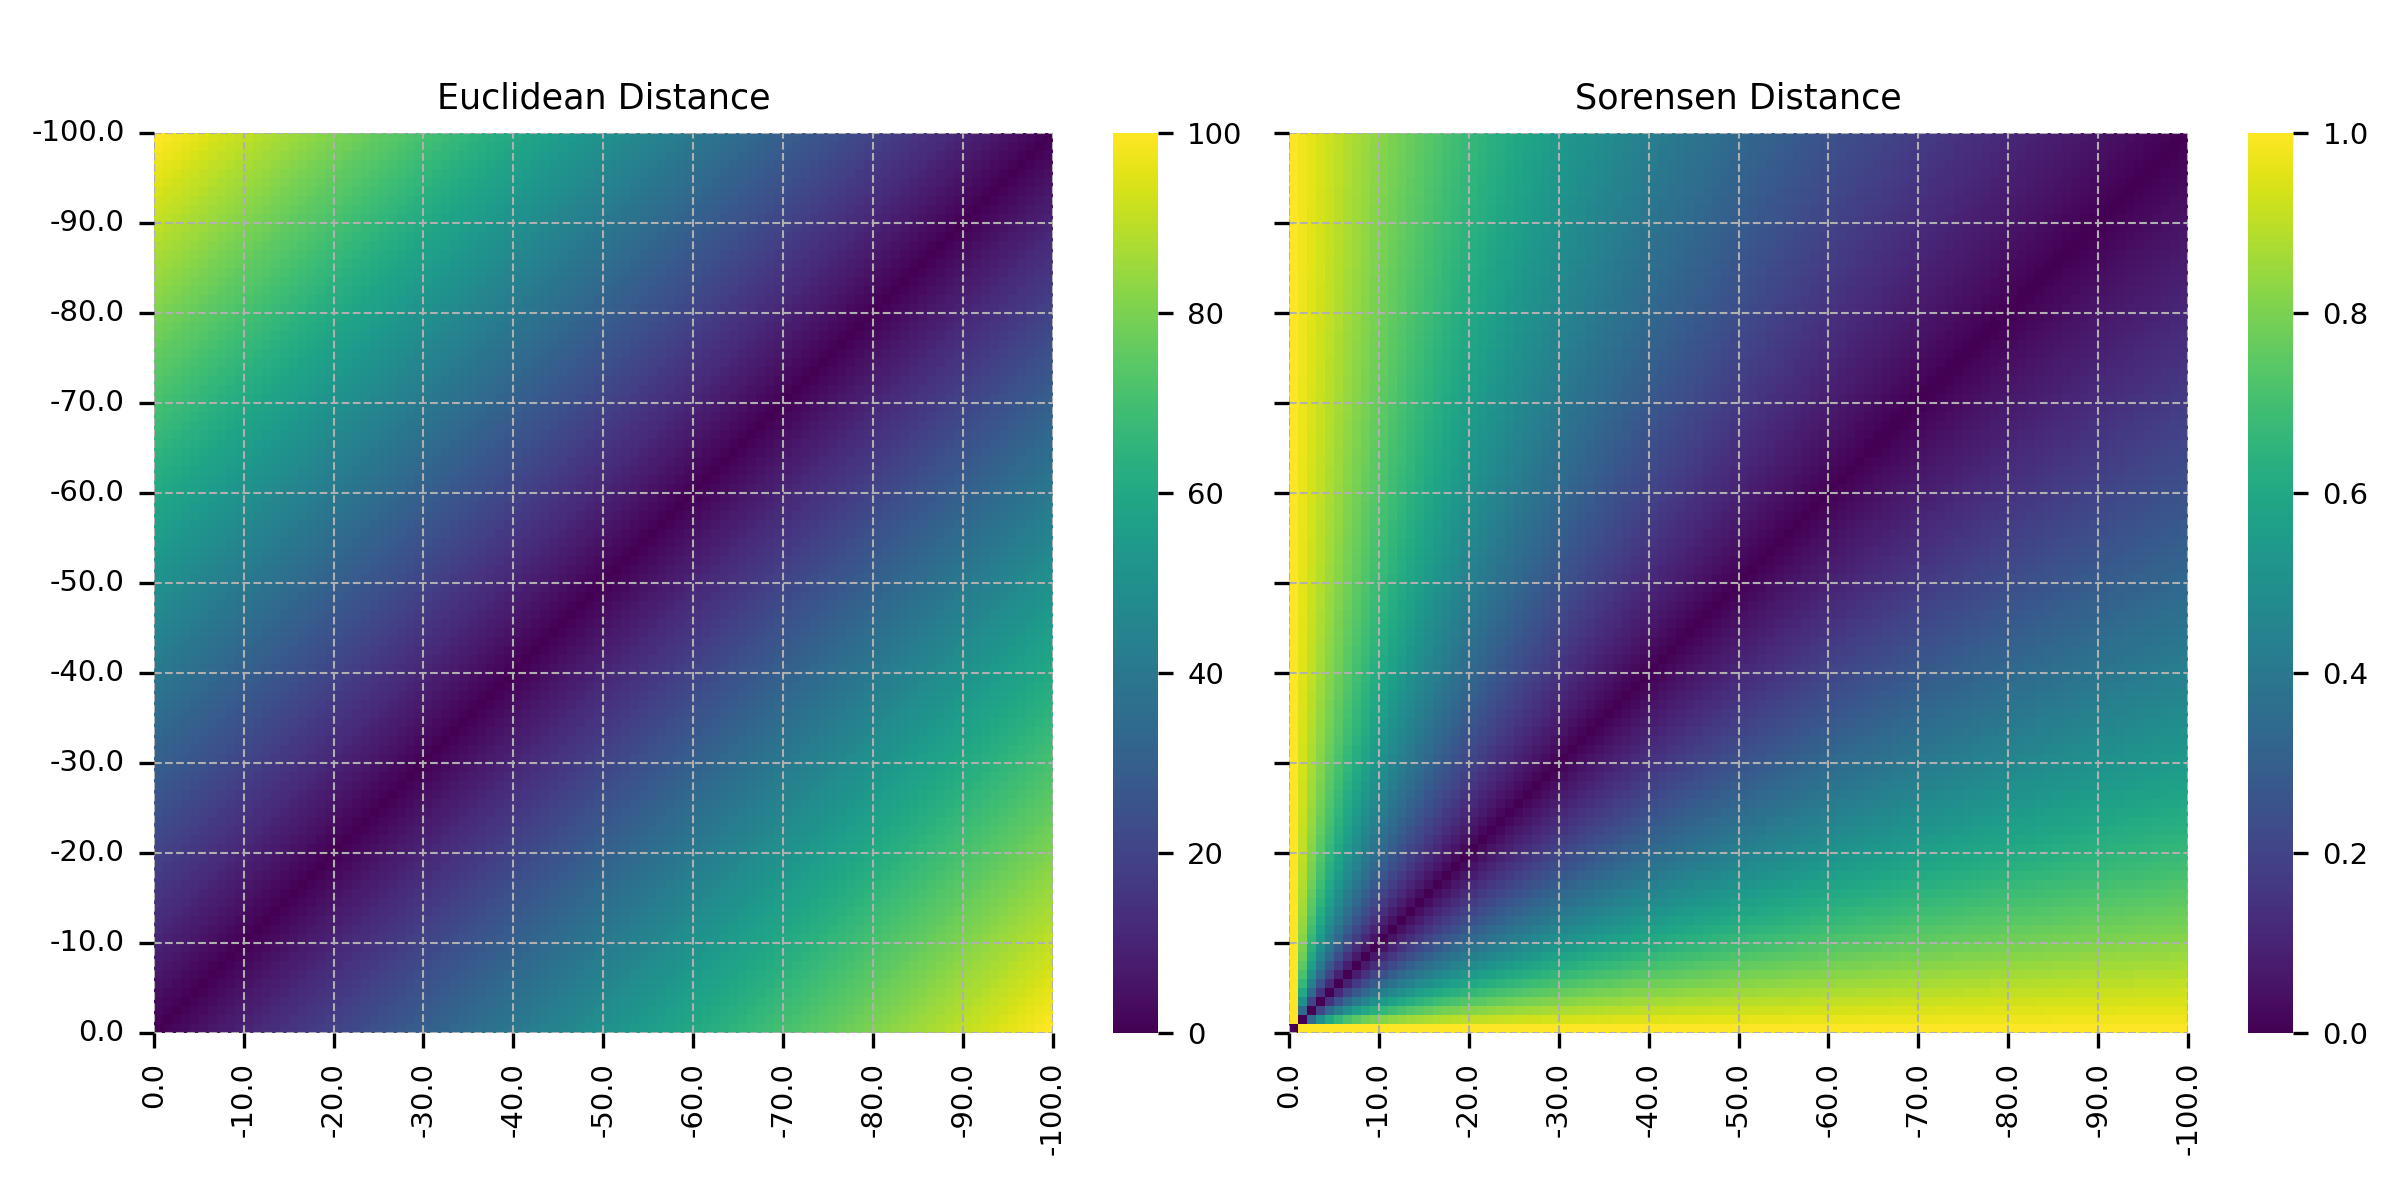
\includegraphics[width=0.8\textwidth]{images/plot_euclidean_vs_sorensen.png}
    \caption{Vergleich der Distanzmetriken Euklidisch und Sørensen}
    \label{fig:distance_metrics_heatmaps}
\end{figure}

\subsection{Anzahl der Nachbarn}

Der Parameter \( k \) legt fest, wie viele nächste Nachbarn für die Klassifizierung berücksichtigt werden. Kleine Werte für \( k \) können zu hoher Varianz und geringer Verzerrung führen, während größere Werte die Varianz verringern, jedoch die Verzerrung erhöhen. Die Wahl des optimalen \( k \)-Werts hängt stark von den vorhandenen Trainingsdaten ab. Bei Daten mit Ausreißern oder Rauschen empfiehlt es sich, höhere \( k \)-Werte zu wählen, da diese in solchen Fällen bessere Ergebnisse liefern. Um Gleichstände bei dem Mehrheitsvotum zu vermeiden, sollten ungerade Werte für \( k \) bevorzugt werden.\mycitefoot{ibmknearestNeighbors}

Bei einem Wert von \( k = 3 \) würden für beide Distanzen in dem Beispiel die Werte der vierten, fünften und sechsten Messung für die Vorhersage verwendet werden, da für diese drei Messungen die Distanzen am geringsten sind (siehe Tabelle \ref{tab:distanzen}) und das Modell würde Raum C vorhersagen, da dieser unter den drei Messungen am häufigsten vertreten ist.

\subsection{Gewichtung}

Der \gls{knn}-Algorithmus kann erweitert werden, indem die Distanzen der \( k \) nächsten Nachbarn nach ihrer Berechnung gewichtet werden. Hierfür stehen verschiedene Gewichtungsfunktionen, wie zum Beispiel der Inversions-Kernel oder der Gauss-Kernel, zur Verfügung. Für Vorhersage unter Verwendung einer Gewichtungsfunktion, werden die Distanzen der \( k \) nächsten Nachbarn nach ihrer Berechnung in die Gewichtungsfunktion eingesetzt, für jede vertretene Klasse aufsummiert und es wird die Klasse mit dem größten Gewicht ausgewählt. Dadurch hat neben der relativen Häufigkeit der Klassen auch die Distanz der Nachbarn einen Einfluss auf die Klassifikation und es ist möglich eine nicht optimale Wahl des Parameters \( k \) auszugleichen.\myfootcite{Hechenbichler2004WeightedKNN}{S. 6}

In dieser Arbeit wurde sich dafür entschieden den Inversions-Kernel zu verwenden, da für die Implementierung des \gls{knn}-Algorithmus die Bibliothek \textit{scikit-learn} verwendet wird und der Inversions-Kernel der Standardgewichtungsfunktion dieser entspricht. Zudem hat die Wahl der Gewichtungsfunktion laut dem Paper \textit{Weighted k-Nearest-Neighbor Techniques and Ordinal Classification} in der Regel keinen entscheidenden Einfluss auf die Genauigkeit der Klassifikation.\myfootcite{Hechenbichler2004WeightedKNN}{S. 6}\textsuperscript{,}\mycitefoot{scikitlearnKNeighborsRegressor}

Die Gewichtungsfunktion des Inversions-Kernels ist gegeben durch:

\begin{equation}
    \label{eq:inversion}
    K(d) = \frac{1}{|d|}
\end{equation}

wobei \( d \) die Distanz darstellt. 

% Quelle für scikit-learn https://scikit-learn.org/stable/modules/generated/sklearn.neighbors.KNeighborsRegressor.html#sklearn.neighbors.KNeighborsRegressor

% Ein Vorteil dieser Gewichtung ist, dass so eine schlechte Wahl des Parameters k wieder ausgeglichen werden kann, da bei einem zu großen Wert für k 

% Wahl der Gewichtungsfunktion nicht sehr ausschlaggebend (Quelle 5, Seite 5, "But from experience the choice of a special kernel (apart from the special case of the rectangular kernel, that gives equal weights to all neighbors) is not crucial.")

\begin{table}[h]
    \centering
    \begin{tabularx}{\textwidth}{|X|X|X|X|}
        \hline
        Raum & Gewicht (Euklidisch) & Gewicht (Sørensen) \\ \hline
        C & 0,671 (0,385 + 0,286) & 116,667 (66,667 + 50) \\ \hline
        B & 0.222 & 33.333 \\ \hline
    \end{tabularx}
    \caption{Gewichtete Distanzen der drei nächstgelegenen Trainingsdaten}
    \label{tab:gewichtete_distanzen}
\end{table}

Unter Verwendung der Gewichtungsfunktion des Inversions-Kernels ergeben sich für das Beispiel die in Tabelle \ref{tab:gewichtete_distanzen} dargestellten gewichteten Distanzen und das Modell würde Raum C vorhersagen.

Für die detaillierten Untersuchungen in Kapitel \ref{untersuchungen} wurde sich dafür entscheiden den \gls{knn}-Algorithmus ohne Gewichtungsfunktion (\texttt{weights = uniform}) und mit Gewichtungsfunktion (\texttt{weights = distance}) zu vergleichen, um zu untersuchen, ob die Gewichtungsfunktion die Genauigkeit der Klassifikation verbessern kann.

\section{Support Vector Machines (SVM)}


% In Abbildung \ref{fig:myplot_7_svm} ist ein SVM dargestellt.

% \begin{figure}[H]
%     \centering
%     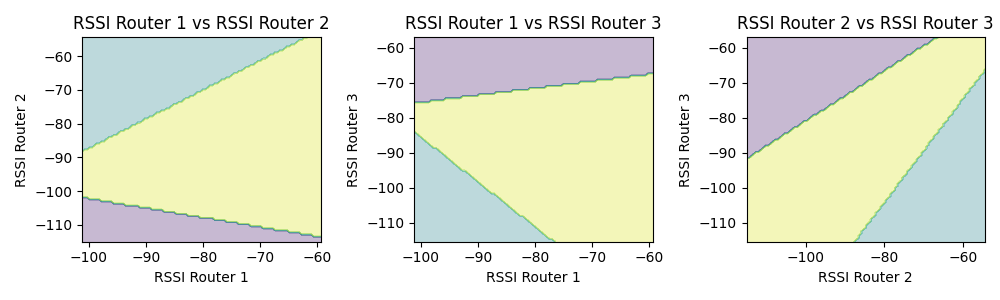
\includegraphics[width=0.8\textwidth]{images/myplot_7_svm.png}
%     \caption{SVM}
%     \label{fig:myplot_7_svm}
% \end{figure}

% \textbf{Quellen:} \\
% \href{https://www.bigdata-insider.de/was-ist-eine-support-vector-machine-a-880134}{Quelle 6: https://www.bigdata-insider.de/was-ist-eine-support-vector-machine-a-880134} \\ % bigdatainsiderEineSupport
% \href{https://www.ibm.com/topics/support-vector-machine}{Quelle 7: https://www.ibm.com/topics/support-vector-machine} \\ % ibmWhatSupport
% \href{https://wires.onlinelibrary.wiley.com/doi/full/10.1002/wics.49}{Quelle 8: https://wires.onlinelibrary.wiley.com/doi/full/10.1002/wics.49} % Mammone2009SVM


% Quelle warum gerade RBF: An Indoor Localization of WiFi Based on Support Vector Machines

% \subsection{Algorithmusbeschreibung}

Der Support Vector Machine (SVM) Algorithmus ist ein maschineller Lernalgorithmus, der für die Klassifizierung von Daten verwendet werden kann. Die Klassifizierung erfolgt, indem versucht wird die optimale Trennlinie – die sogenannte Hyperebene – zwischen den Datenpunkten zu finden. Die Hyperebene wird dabei so positioniert, dass der Abstand zwischen den Datenpunkten der beiden Klassen maximiert wird. In einem Beispiel mit zwei Merkmalen, wie in Abbildung \ref{fig:svm_hyperplane}, lassen sich die Datenpunkte beider Klassen in einem zweidimensionalen Koordinatensystem als Punkte darstellen und die Hyperebene als Linie. 

Der \gls{svm} Algorithmus ist auch in der Lage mit mehr als zwei Merkmalen zu arbeiten, indem versucht wird eine Hyperebene in einem mehrdimensionalen Raum, welche die Datenpunkte der verschiedenen Klassen voneinander trennt, zu finden.\mycitefoot{ibmWhatSupport}

\begin{figure}[H]
    \centering
    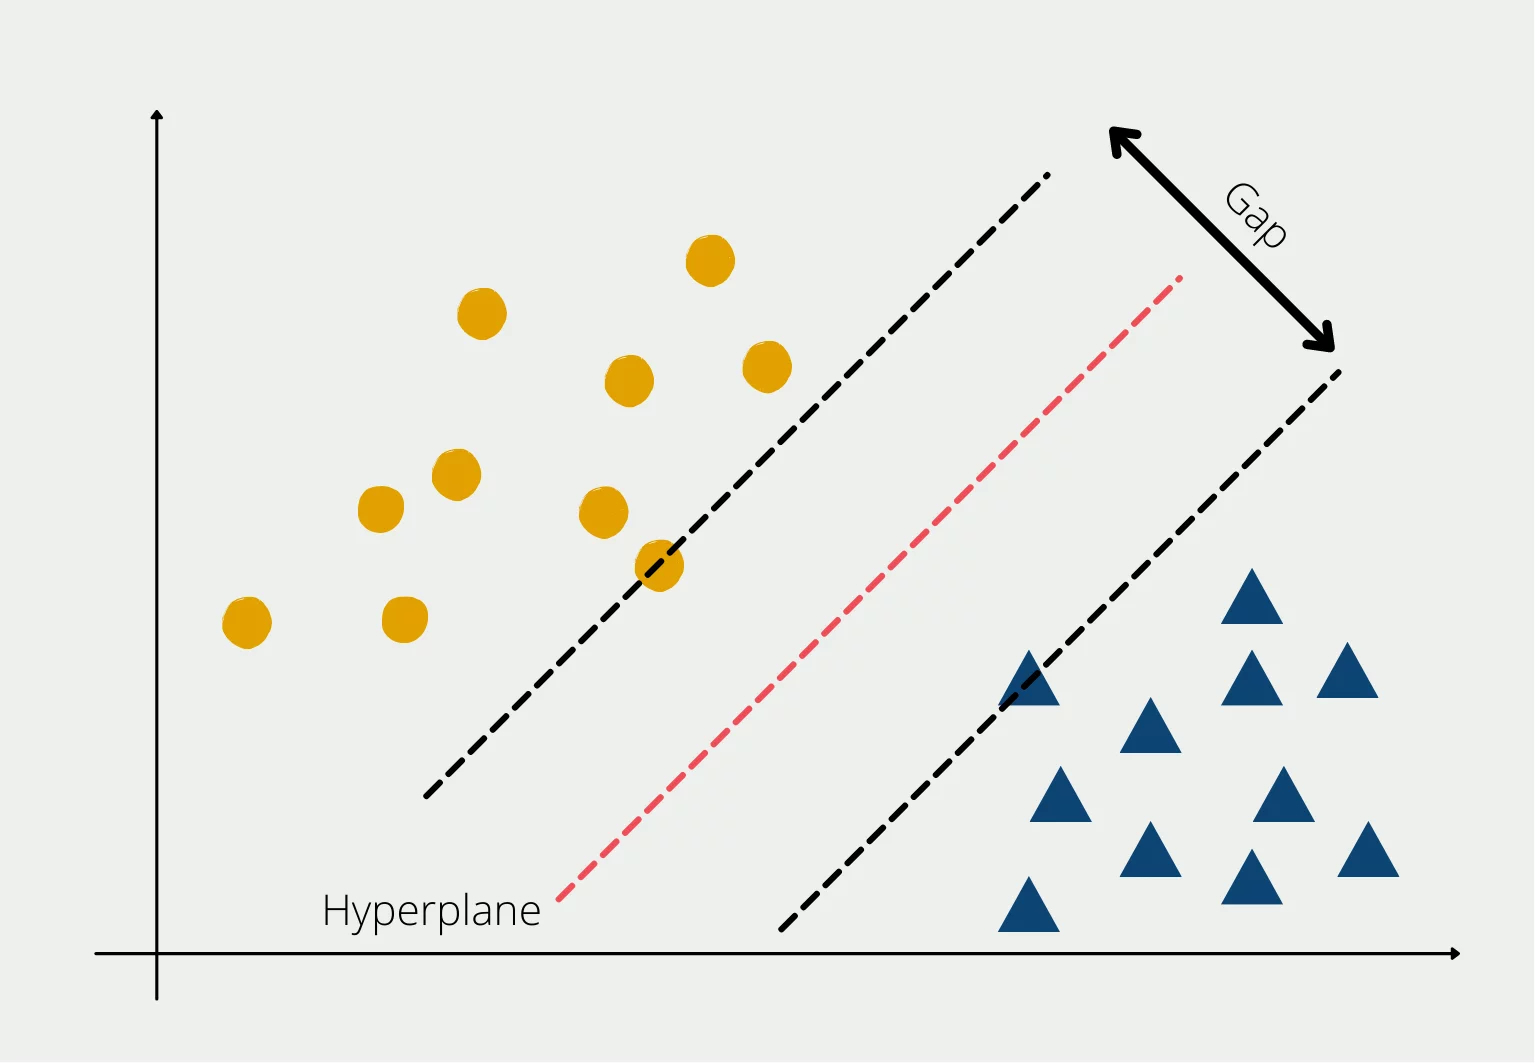
\includegraphics[width=0.4\textwidth]{images/source_svm.png}
    \caption{Darstellung einer Hyperebene in einem \gls{svm} mit zwei Features (Bildquelle: \citeauthor{databasecampSupportVector} \citeyear{databasecampSupportVector})}
    \label{fig:svm_hyperplane}
\end{figure}

\subsection{Auswahl des Kernels}

In Abbildung \ref{fig:svm_hyperplane} konnten die Daten durch eine Gerade getrennt werden, weswegen ein \gls{svm} mit einem linearen Kernel verwendet werden konnte. Sollten die Daten nicht linear trennbar sein - wie in Abbildung \ref{fig:source_svm_rbf} - sollte ein anderer Kernel verwendet werden. In diesen Fällen wird zuerst die Kernel-Methode angewendet, welche die Daten in einen höherdimensionalen Raum transformiert, und anschließend wird versucht die Daten in diesem Raum linear zu trennen.\mycitefoot{ibmWhatSupport}

In dieser Arbeit wurde sich dafür entschieden, den linearen Kernel mit einem nicht linearen Kernel zu vergleichen. Für das nicht lineare \gls{svm} wurde der RBF-Kernel gewählt, da in der Arbeit \textit{Device-Free Presence Detection and Localization With SVM and CSI Fingerprinting} mit diesem Kernel die besten Ergebnisse unter den nicht linearen SVMs erzielt werden konnten.\mycitefoot{ibmWhatSupport}

\begin{figure}[H]
    \centering
    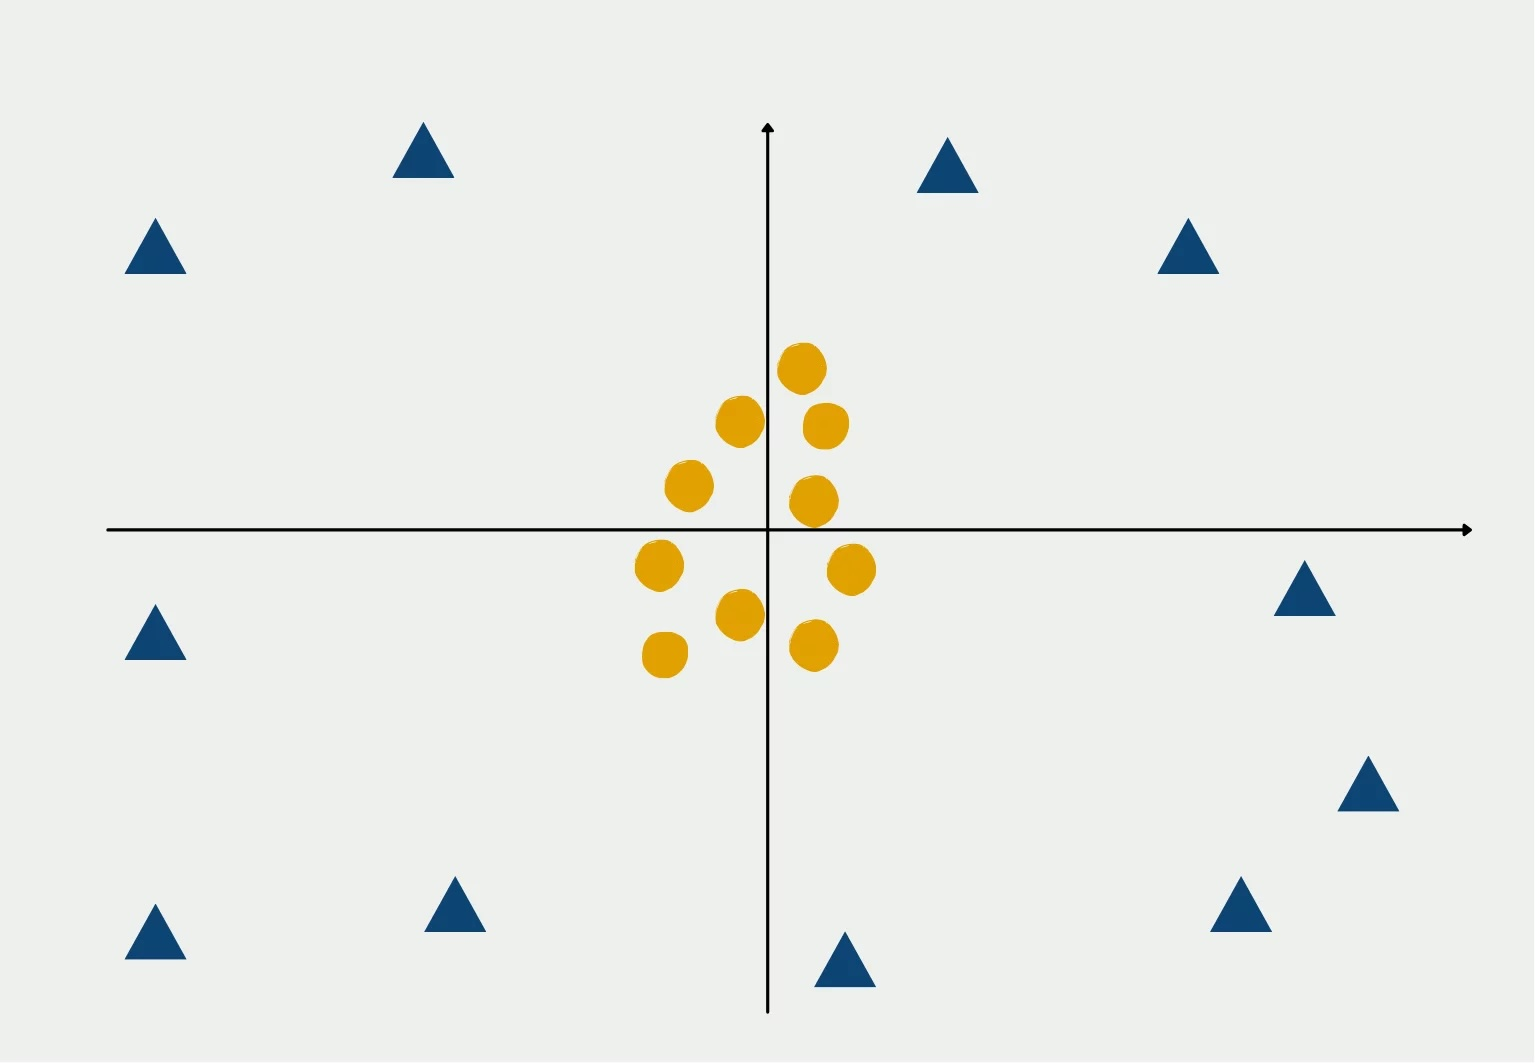
\includegraphics[width=0.4\textwidth]{images/source_svm_rbf.png}
    \caption{Darstellung von nicht linear trennbaren Daten in einem \gls{svm} (Bildquelle: \citeauthor{databasecampSupportVector} \citeyear{databasecampSupportVector})}
    \label{fig:source_svm_rbf}
\end{figure}

\subsection{Regularisierungsparameter C und Kernel-Parameter \texttt{gamma}}

% TODO: Margin erklären -> bereich in dem die Hyperebene liegt und bessere Bilder (Dort steht Gap...)

Der \gls{svm} Algorithmus kann über den Regularisierungsparameter C und den Kernel-Parameter \texttt{gamma} konfiguriert werden. Der Regularisierungsparameter C legt dabei fest, wie groß der Bereich ist, in dem die Hyperebene liegt. Also der Abstand zwischen den beiden schwarzen Linien in Abbildung \ref{fig:svm_hyperplane}. Je kleiner der Wert ist, desto größer ist der Abstand. Größere Werte für C können dazu führen, dass das Modell die Trainingsdaten gut klassifizieren kann, jedoch kann das auch dazu führen, dass das Modell fehleranfälliger bei der Klassifikation neuer Daten ist.\mycitefoot{baeldungParameterSupport}

Der Kernel-Parameter \texttt{gamma} kann nur für nicht lineare \gls{svm}-Modelle verwendet werden und legt fest, wie groß der Einfluss eines einzelnen Trainingsbeispiels bei der Berechnung der Hyperebene ist. Bei einem großen Wert für \texttt{gamma} ist der Einfluss eines einzelnen Trainingsbeispiels gering und es kann zum Overfitting. Dies bedeutet das dass Modell die Trainingsdaten zu stark berücksichtigt und neue Daten nicht so gut klassifizieren kann. Ein kleiner Wert für \texttt{gamma} kann dazu führen, dass das Modell zu stark vereinfacht wird und es zum Underfitting kommt.\mycitefoot{geeksforgeeksGammaParameter}

% Quelle für die Auswahl der Parameter Werte: Semi-Supervised Classification by Low Density Separation

\section{Random Forest}

% Gute quelle: WiFi Indoor Localization with CSI Fingerprinting-Based Random Forest -> Wie wichtig ist welcher Hyperparameter? % Wang2018WiFiLocalization

% In Abbildung \ref{fig:myplot_7_rf} ist ein Entscheidungsbaum dargestellt.

% \begin{figure}[H]
%     \centering
%     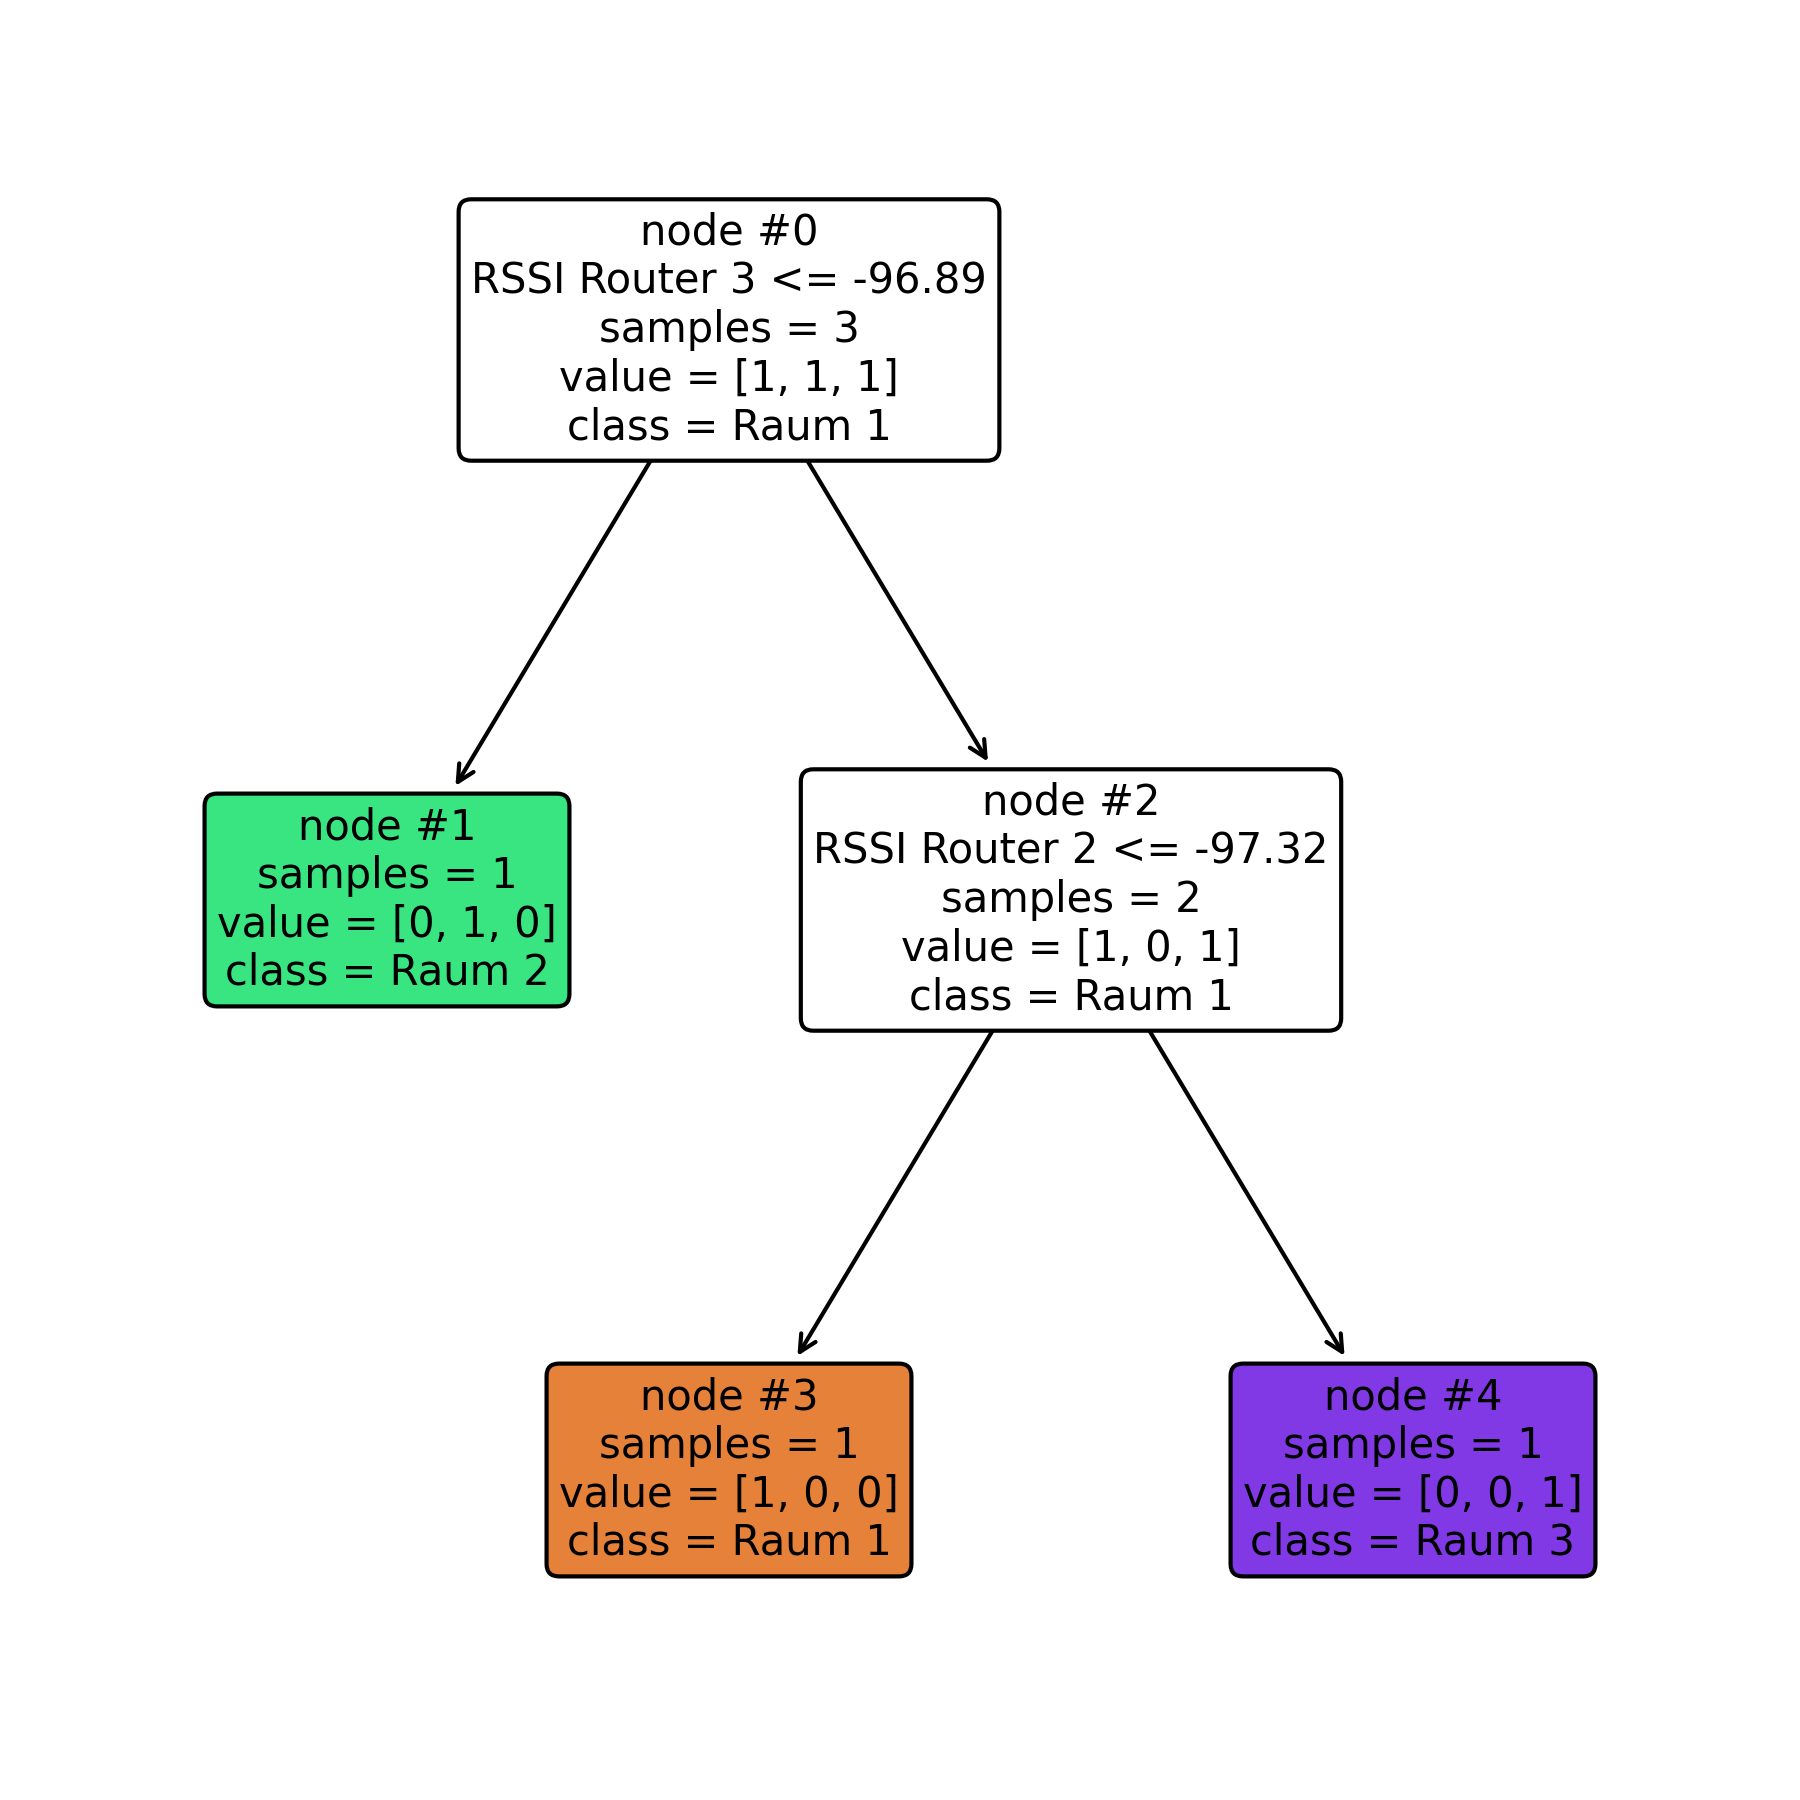
\includegraphics[width=0.8\textwidth]{images/myplot_7_rf.png}
%     \caption{Distance vs. Uniform weights}
%     \label{fig:myplot_7_rf}
% \end{figure}

% \textbf{Quelle:} \\
% \href{https://builtin.com/data-science/random-forest-algorithm}{Quelle 9: https://builtin.com/data-science/random-forest-algorithm} % builtinRandomForest

% \subsection{Algorithmusbeschreibung}

Der Random Forest-Algorithmus ist Lernalgorithmus der zur Klassifizierung verwendet werden kann. Dabei basiert die Vorhersage auf einer Vielzahl von Entscheidungsbäumen, die jeweils eine eigene Vorhersage treffen. Ein Entscheidungsbaum ist ein Modell, das Entscheidungen durch eine Abfolge von Wahl/Falsch-Abfragen trifft, die sich aus den Merkmalen der Daten ableiten. An jedem Knotenpunkt des Baumes wird eine Entscheidung basierend auf einem einzelnen Merkmal getroffen und am Ende eines jeden Entscheidungsbaums erfolgt eine Vorhersage. 

Für jeden Entscheidungsbaum im Random Forest wird eine zufällige Teilmenge der Trainingsdaten verwendet und die endgültige Vorhersage des Random Forests Modells ergibt sich aus einem Mehrheitsvotum der individuellen Entscheidungsbäume.\mycitefoot{builtinRandomForest}

Laut der Studie \textit{WiFi Indoor Localization with CSI Fingerprinting-Based Random Forest} sind die einflussreichsten Parameter des Random Forest Algorithmus die maximale Tiefe der Bäume (\texttt{max\_depth}), die Anzahl der Entscheidungsbäume (\texttt{n\_estimators}) sowie die maximale Anzahl der betrachteten Features (\texttt{max\_features}). Aus diesem Grund werden in dieser Arbeit diese Parameter in Bezug auf die Genauigkeit bei der Vorhersage untersucht.\myfootcite{Wang2018WiFiLocalization}{S. 18}

In Abbildung \ref{fig:random_forest} ist ein Entscheidungsbaum dargestellt, welcher mit Hilfe der Beispieldaten aus Tabelle \ref{tab:trainingsdaten} erstellt wurde und für die Daten aus Tabelle \ref{tab:testdaten} Raum C vorhersagen würde.

\begin{figure}[H]
    \centering
    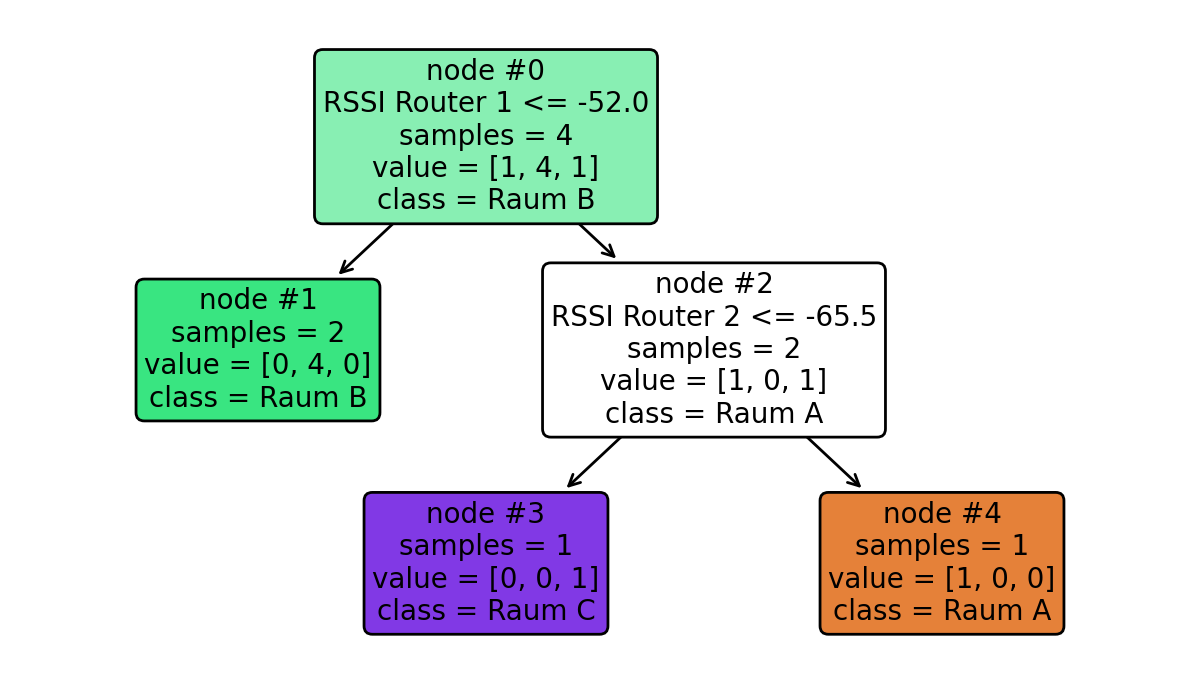
\includegraphics[width=0.4\textwidth]{images/random_forest.png}
    \caption{Darstellung eines Entscheidungsbaums anhand der Beispieldaten}
    \label{fig:random_forest}
\end{figure}


% \subsection{Parameter: Anzahl der Bäume (n\_estimators)}

\chapter{Systemarchitektur und Implementierung} \label{implementierung}
% Der \gls{accesspoint} sendet die \gls{bssid} und die \gls{ssid}, damit Geräte, wie eine \gls{vm}, sich verbinden können. Algorithmen wie \gls{knn} und \gls{svm} können in einer \gls{api} implementiert werden, um die Datenverarbeitung zu optimieren.

Die implementierte Software lässt sich in vier Komponenten unterteilen: Die Android App \textit{BVG Detection}, welche bereits in einer vorherigen Arbeit entwickelt wurde\myfootcite{winter2017indoor}{S. 11 ff.}, einem Server der eine API bereitstellt, welche die in der Offline-Phase gesammelten Daten speichern kann und für WiFi-Fingerprints von unbekannten Räumen eine Vorhersage treffen kann, einer Datenbank zur Verwaltung der Fingerprints und dem Quellcode der Microcontroller.

\section{Datenbankstruktur} \label{datenbank}

Für die Speicherung der gesammelten WiFi-Fingerprints während der Offline-Phase wurde eine Datenbankstruktur entwickelt, welche auf einer \textit{MariaDB}-Instanz auf dem Server und in einer \textit{SQLite}-Datenbank innerhalb der App \textit{BVG Detection} implementiert wurde. Die Datenbank besteht aus den vier Tabellen \texttt{rooms}, \texttt{measurements}, \texttt{routers} und \texttt{measurement\_router}.

\subsection{Tabelle \texttt{rooms}}

In der Tabelle \texttt{rooms} werden die Informationen der Räume, in denen die Messungen durchgeführt wurden, gespeichert. Dazu gehören eine eindeutige Raum-ID, der Name des Raumes, eine Beschreibung,  Koordinaten und der Pfad zu einer Bilddatei. Die Beschreibung, die Koordinaten und der Pfad der Bilddatei sind dabei nur für die \textit{BVG Detection}-App relevant.

\begin{table}[h]
    \centering
    \begin{tabularx}{\textwidth}{|l|l|X|}
        \hline
        \textbf{Spalte} & \textbf{Datentyp} & \textbf{Beschreibung} \\ \hline
        room\_id & INT & Primärschlüssel der Tabelle \\ \hline
        room\_name & VARCHAR(255) & Eindeutiger Name des Raumes \\ \hline
        description & VARCHAR(255) & Beschreibung des Raumes \\ \hline
        coordinates & VARCHAR(255) & Geografische Koordinaten des Raumes \\ \hline
        picture\_path & VARCHAR(255) & Pfad zu einer Bilddatei des Raumes \\ \hline
    \end{tabularx}
    \caption{Struktur der Tabelle \texttt{rooms}.}
    \label{tab:rooms}
\end{table}

\subsection{Tabelle \texttt{measurements}}

Die Tabelle \texttt{measurements} dient der Erfassung aller Messungen. Jede Messung wird durch eine eindeutige Kombination aus Geräte-ID und Zeitstempel identifiziert, um doppelte Einträge zu vermeiden. Das ist wichtig, da in einer Datenbank auch die Messungen mehrerer Geräte vorhanden sein können und diese unterschieden werden müssen. Zudem wird die Raum-ID gespeichert, die auf die Tabelle \texttt{rooms} verweist, wodurch die Messung einem Raum zugeordnet werden kann.

\begin{table}[h]
    \centering
    \begin{tabularx}{\textwidth}{|l|l|X|}
        \hline
        \textbf{Spalte} & \textbf{Datentyp} & \textbf{Beschreibung} \\ \hline
        measurement\_id & INT & Primärschlüssel der Tabelle \\ \hline
        timestamp & TIMESTAMP & Zeitpunkt der Messung \\ \hline
        device\_id & VARCHAR(255) & ID des Gerätes, das die Messung durchgeführt hat \\ \hline
        room\_id & INT & Verweis auf den Raum, in dem die Messung stattfand \\ \hline
    \end{tabularx}
    \caption{Struktur der Tabelle \texttt{measurements}.}
    \label{tab:measurements}
\end{table}

\subsection{Tabelle \texttt{routers}}

In der Tabelle \texttt{routers} werden die Informationen der erfassten Access Points gespeichert. Die Einträge der Spalte \textit{BSSID} werden dazu verwendet, um zu überprüfen, ob ein Access Point bereits in der Tabelle gespeichert ist, da die \textit{BSSID} jeden Access Point eindeutig kennzeichnet.

\begin{table}[h]
    \centering
    \begin{tabularx}{\textwidth}{|l|l|X|}
        \hline
        \textbf{Spalte} & \textbf{Datentyp} & \textbf{Beschreibung} \\ \hline
        router\_id & INT  & Primärschlüssel der Tabelle \\ \hline
        ssid & VARCHAR(255) & Name des WiFi-Netzwerks (SSID) \\ \hline
        bssid & VARCHAR(255) & MAC-Adresse des Routers (BSSID) \\ \hline
    \end{tabularx}
    \caption{Struktur der Tabelle \texttt{routers}.}
    \label{tab:routers}
\end{table}

\subsection{Tabelle \texttt{measurement\_router}}


Die Tabelle \textit{measurement\_router} speichert die empfangenen Signalstärken der Access Points aller Messungen und verknüpft diese über den Eintrag \textit{measurement\_id} mit den Einträgen aus der Tabelle \textit{measurements}. 

\begin{table}[h]
    \centering
    \begin{tabularx}{\textwidth}{|l|l|X|}
        \hline
        \textbf{Spalte} & \textbf{Datentyp} & \textbf{Beschreibung} \\ \hline
        measurement\_id & INT & Verweis auf eine Messung \\ \hline
        router\_id & INT & Verweis auf einen Router \\ \hline
        signal\_strength & INT & Empfangene Signalstärke bei der Messung \\ \hline
    \end{tabularx}
    \caption{Struktur der Tabelle \texttt{measurement\_router}.}
    \label{tab:measurement_router}
\end{table}

\section{Implementierung des Servers} \label{api}

% Quelle: https://dev.to/ken_mwaura1/getting-started-monitoring-a-fastapi-app-with-grafana-and-prometheus-a-step-by-step-guide-3fbn

Der Server läuft auf einer virtuellen Maschine der HTW Berlin unter der Linux Distribution \textit{Debain}, ist mit 2 CPU-Kernen, 3 GB RAM und einem Speicherplatz von 16 GB konfiguriert und ist über die IP-Adresse \texttt{141.45.212.246} aus dem Netzwerk der HTW erreichbar. Auf diesem Server sind vier zentrale Anwendungen in separaten Docker-Containern implementiert: eine \textit{FastAPI}-Anwendung, \textit{Prometheus}, \textit{Grafana} und \textit{MariaDB}. Diese Anwendungen können mithilfe von \textit{Docker Compose} über den Befehl \texttt{sudo docker-compose build} installiert werden und über \texttt{sudo docker-compose up -d} und \texttt{sudo docker-compose down} gestartet bzw. beendet werden. Das bietet den Vorteil, dass alle Anwendungen ohne großen Aufwand installiert werden können und die Abhängigkeiten der Anwendungen korrekt konfiguriert sind. Die Implementierung des Servers basiert auf der Anleitung von \textit{Zoo Codes}.\mycitefoot{devGettingStarted}

\subsection{FastAPI} \label{section-fastapi}

% Verwendet: sqlalchemy

% Quelle Vorteile FastAPI https://www.netguru.com/blog/python-flask-versus-fastapi
Die API zur Verwaltung von WiFi-Fingerprints und zur Vorhersage von Räumen basierend auf WiFi-Fingerprints von nicht bekannten Räumen wurde mithilfe des Python-Frameworks \textit{FastAPI} implementiert. \textit{FastAPI} bietet den Vorteil, dass automatisch eine interaktive API-Dokumentation (aufrufbar unter \texttt{http://141.45.212.246:8000/docs}) bereitgestellt wird (siehe Abbildung \ref{fig:fast_api_screenshot}), die es ermöglicht, die Endpunkte der API zu testen.

\begin{figure}[h]
    \centering
    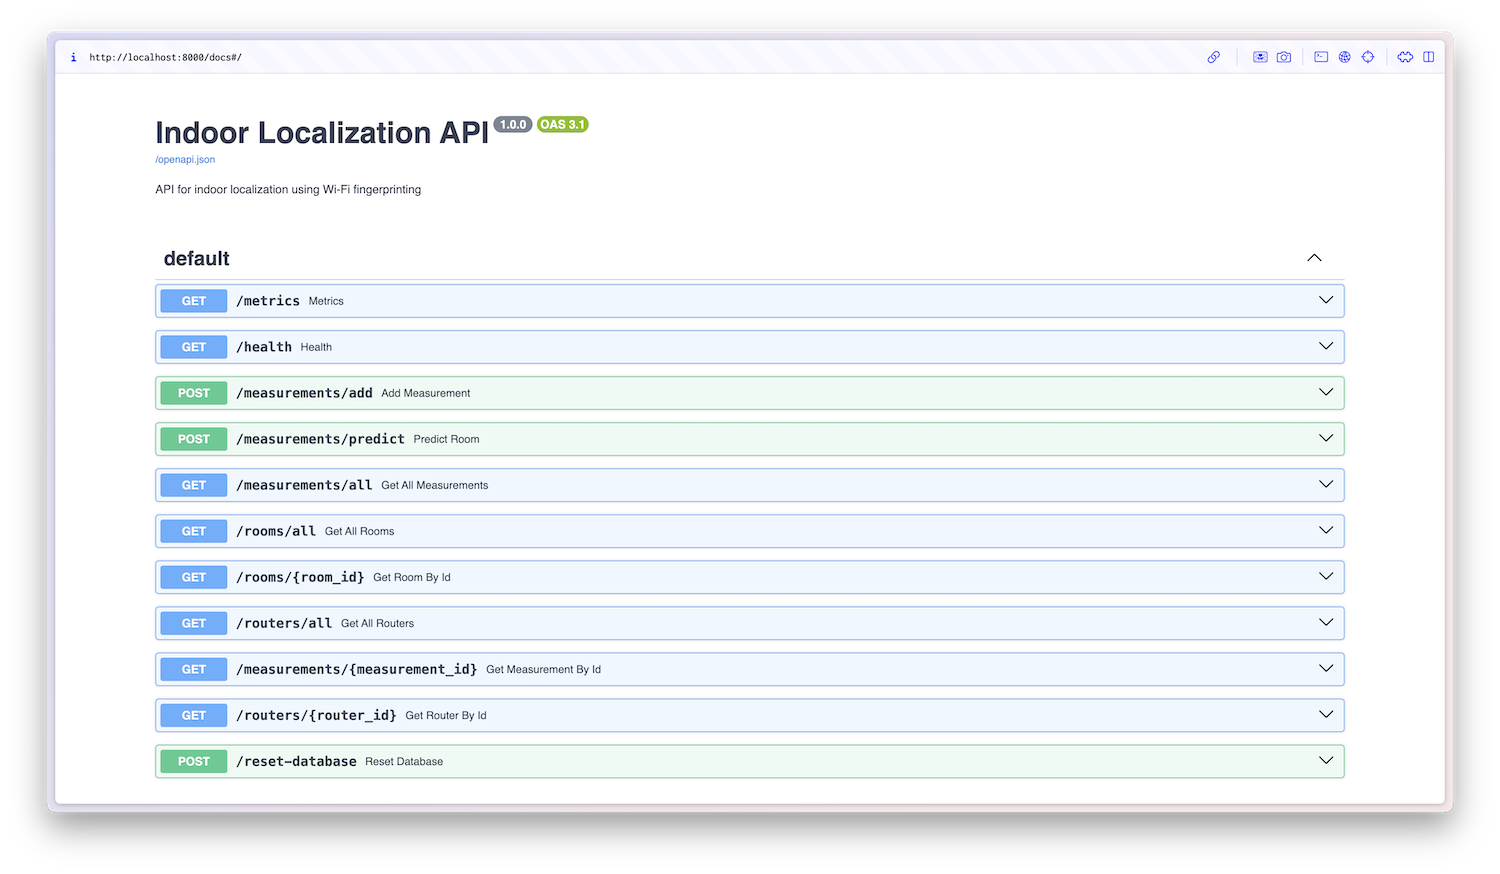
\includegraphics[width=0.8\textwidth]{images/screenshots/api_docs.png}
    \caption{FastAPI Dokumentation}
    \label{fig:fast_api_screenshot}
\end{figure}

Die API stellt verschiedene Routen zur Verfügung, welche in Tabelle \ref{tab:api_routes} aufgelistet sind.

\begin{table}[h]
    \centering
    \begin{tabularx}{\textwidth}{|l|l|X|}
    \hline
    \textbf{Route} & \textbf{Methode} & \textbf{Beschreibung} \\ \hline
    \texttt{/health} & \texttt{GET} & Prüft den Status der API. \\ \hline
    \texttt{/measurements/add} & \texttt{POST} & Fügt eine neue Messung hinzu. \\ \hline
    \texttt{/measurements/predict} & \texttt{POST} & Sagt den Raum basierend auf Wi-Fi-Daten voraus. \\ \hline
    \texttt{/measurements/all} & \texttt{GET} & Ruft alle gespeicherten Messungen ab. \\ \hline
    \texttt{/measurements/\{measurement\_id\}} & \texttt{GET} & Ruft eine spezifische Messung nach ID ab. \\ \hline
    \texttt{/rooms/all} & \texttt{GET} & Ruft alle gespeicherten Räume ab. \\ \hline
    \texttt{/rooms/\{room\_id\}} & \texttt{GET} & Ruft einen spezifischen Raum nach ID ab. \\ \hline
    \texttt{/routers/all} & \texttt{GET} & Ruft alle gespeicherten Router ab. \\ \hline
    \texttt{/routers/\{router\_id\}} & \texttt{GET} & Ruft einen spezifischen Router nach ID ab. \\ \hline
    \texttt{/reset-database} & \texttt{POST} & Setzt die Datenbank zurück. \\ \hline
    \end{tabularx}
    \caption{Übersicht der Endpunkte der \textit{FastAPI}-Anwendung.}
    \label{tab:api_routes}
\end{table}

\subsection*{Route: \texttt{/measurements/add}}

Zum Hinzufügen eines neuen WiFi-Fingerprints, der während der Offline-Phase gesammelt wurde, kann die Route \texttt{/measurements/add} verwendet werden. Dabei wird im ersten Schritt überprüft, ob es bereits einen Eintrag in der Tabelle \texttt{measurements} gibt, bei dem die Einträge \texttt{device\_id} und \texttt{timestamp} mit den übergebenen Werten übereinstimmen. Falls ein solcher Eintrag bereits existiert, wird die Messung nicht hinzugefügt. Dadurch kann sichergestellt werden, dass keine doppelten Einträge in der Datenbank vorhanden sind. Sollte die Messung noch nicht in der Datenbank vorhanden sein, wird für diese Messung ein neuer Eintrag in der Tabelle \texttt{measurements} hinzugefügt und für jeden empfangenen Router ein Eintrag in der Tabelle \texttt{measurement\_router} erstellt.

In dem Code Beispiel \ref{lst:add_request} ist eine Beispielanfrage an die Route \texttt{/measurements/add} dargestellt, bei der ein neuer WiFi-Fingerprint für den Raum \texttt{WH\_C\_625} hinzugefügt werden soll.

\begin{lstlisting}[caption={Beispiel für eine Anfrage an \texttt{/measurements/predict}}, label={lst:add_request}]
{
    "room_name": WH_C_625,
    "device_id": google_pixel_8,
    "timestamp": 1721479799,
    "routers": [
        {
            "ssid": "eduroam",
            "bssid": "dc:b8:08:c9:73:02",
            "signal_strength": -73
        }
    ]
}
\end{lstlisting}

\subsection*{Route: \texttt{/measurements/predict}}

Die \texttt{POST} Route \texttt{/measurements/predict} wird verwendet um für einen WiFi-Fingerprint eine Raumvorhersage zu treffen. Dafür wurden die in Kapitel \ref{algorithmen} beschriebenen Algorithmen \gls{knn}, \gls{svm} und Random Forest mit den dazugehörigen Parametern implementiert. Für die Implementierung der Algorithmen wurde die Python Bibliothek \texttt{scikit-learn} verwendet.

Der Endpunkt erwartet unter dem Parameter \texttt{routers} eine Liste von Router Objekten, welche jeweils die Einträge \texttt{ssid}, \texttt{bssid} und \texttt{signal\_strength} beinhalten. Zusätzlich kann über den optionalen Parameter \texttt{algorithm} der Algorithmus zur Vorhersage festgelegt werden (die möglichen Werte hierbei sind \texttt{knn\_euclidean}, \texttt{knn\_sorensen}, \texttt{random\_forest}, \texttt{svm\_rbf} und \texttt{svm\_linear}). Die Algorithmus spezifischen Parameter können über die Parameter \texttt{k\_value}, \texttt{weights}, \texttt{n\_estimators}, \texttt{c\_value}, \texttt{gamma\_value}, \texttt{max\_depth} und \texttt{max\_features} gesetzt werden und entsprechen den Parametern der \texttt{scikit-learn} Bibliothek. Über den Parameter \texttt{ignore\allowbreak\_\allowbreak measurements} können \textit{IDs} von Messungen angegeben werden, die bei der Vorhersage ignoriert werden sollen.

Für die Verwendung der in Kapitel \ref{strategien} untersuchten Datenaufbereitungsmethoden können die Parameter \texttt{use\allowbreak\_remove\allowbreak\_unreceived\allowbreak\_bssids}, \texttt{handle\allowbreak\_missing\allowbreak\_values\allowbreak\_strategy}, \texttt{router\allowbreak\_selection}, \texttt{router\allowbreak\_presence\allowbreak\_threshold}, \texttt{value\allowbreak\_scaling\allowbreak\_strategy} und \texttt{router\allowbreak\_rssi\allowbreak\_thres\-hold} gesetzt werden.

In dem Code Beispiel \ref{lst:predict_request} ist eine Beispielanfrage an die Route \texttt{/measurements/predict} dargestellt, bei der für einen WiFi-Fingerprint bestehend aus zwei Access Points eine Raumvorhersage getroffen werden soll unter Verwendung des \gls{knn}-Algorithmus mit dem Wert 5 für k und ohne Gewichtungsfunktion (\texttt{weights = uniform}).

\begin{lstlisting}[caption={Beispiel für eine Anfrage an \texttt{/measurements/predict}}, label={lst:predict_request}]
{
    "routers": [
        {
            "ssid": "eduroam",
            "bssid": "dc:b8:08:c9:54:a1",
            "signal_strength": -88
        },
        {
            "ssid": "Gast@HTW",
            "bssid": "dc:b8:08:c9:54:a2",
            "signal_strength": -85
        }
    ],
    "algorithm": "knn_euclidean",
    "k_value": 5,
    "weights": "uniform"
}
\end{lstlisting}

Als Antwort liefert die API ein \textit{JSON}-Objekt, das den vorhergesagten Raum zurückgibt.

\begin{lstlisting}[caption={Beispiel einer API-Antwort von \texttt{/measurements/predict}}]
{
  "room_name": "WH_C_625",
}
\end{lstlisting}

\subsection{Grafana und Prometheus}

Neben der Datenbank und der FastAPI-Anwendung wurden auch die Monitoring-Tools \texttt{Pro\discretionary{-}{}{}metheus} und \texttt{Grafana} auf dem Server installiert, um die Leistung der Anwendungen zu überwachen und die Daten in Echtzeit zu visualisieren. Dabei dient Prometheus zur Speicherung der Metriken von der \textit{FastAPI} und \textit{Grafana} zur Visualisierung. Für die Überwachung der \textit{FastAPI} wurde ein Dashboard implementiert, welches die CPU- und RAM-Auslastung, die Anfragen pro Minute nach \textit{HTTP}-Statuscode und die durchschnittliche Antwortzeit für jeden Endpunkt anzeigt (siehe Abbildung \ref{fig:grafana_fast_api_screenshot}).  

\begin{figure}[h]
    \centering
    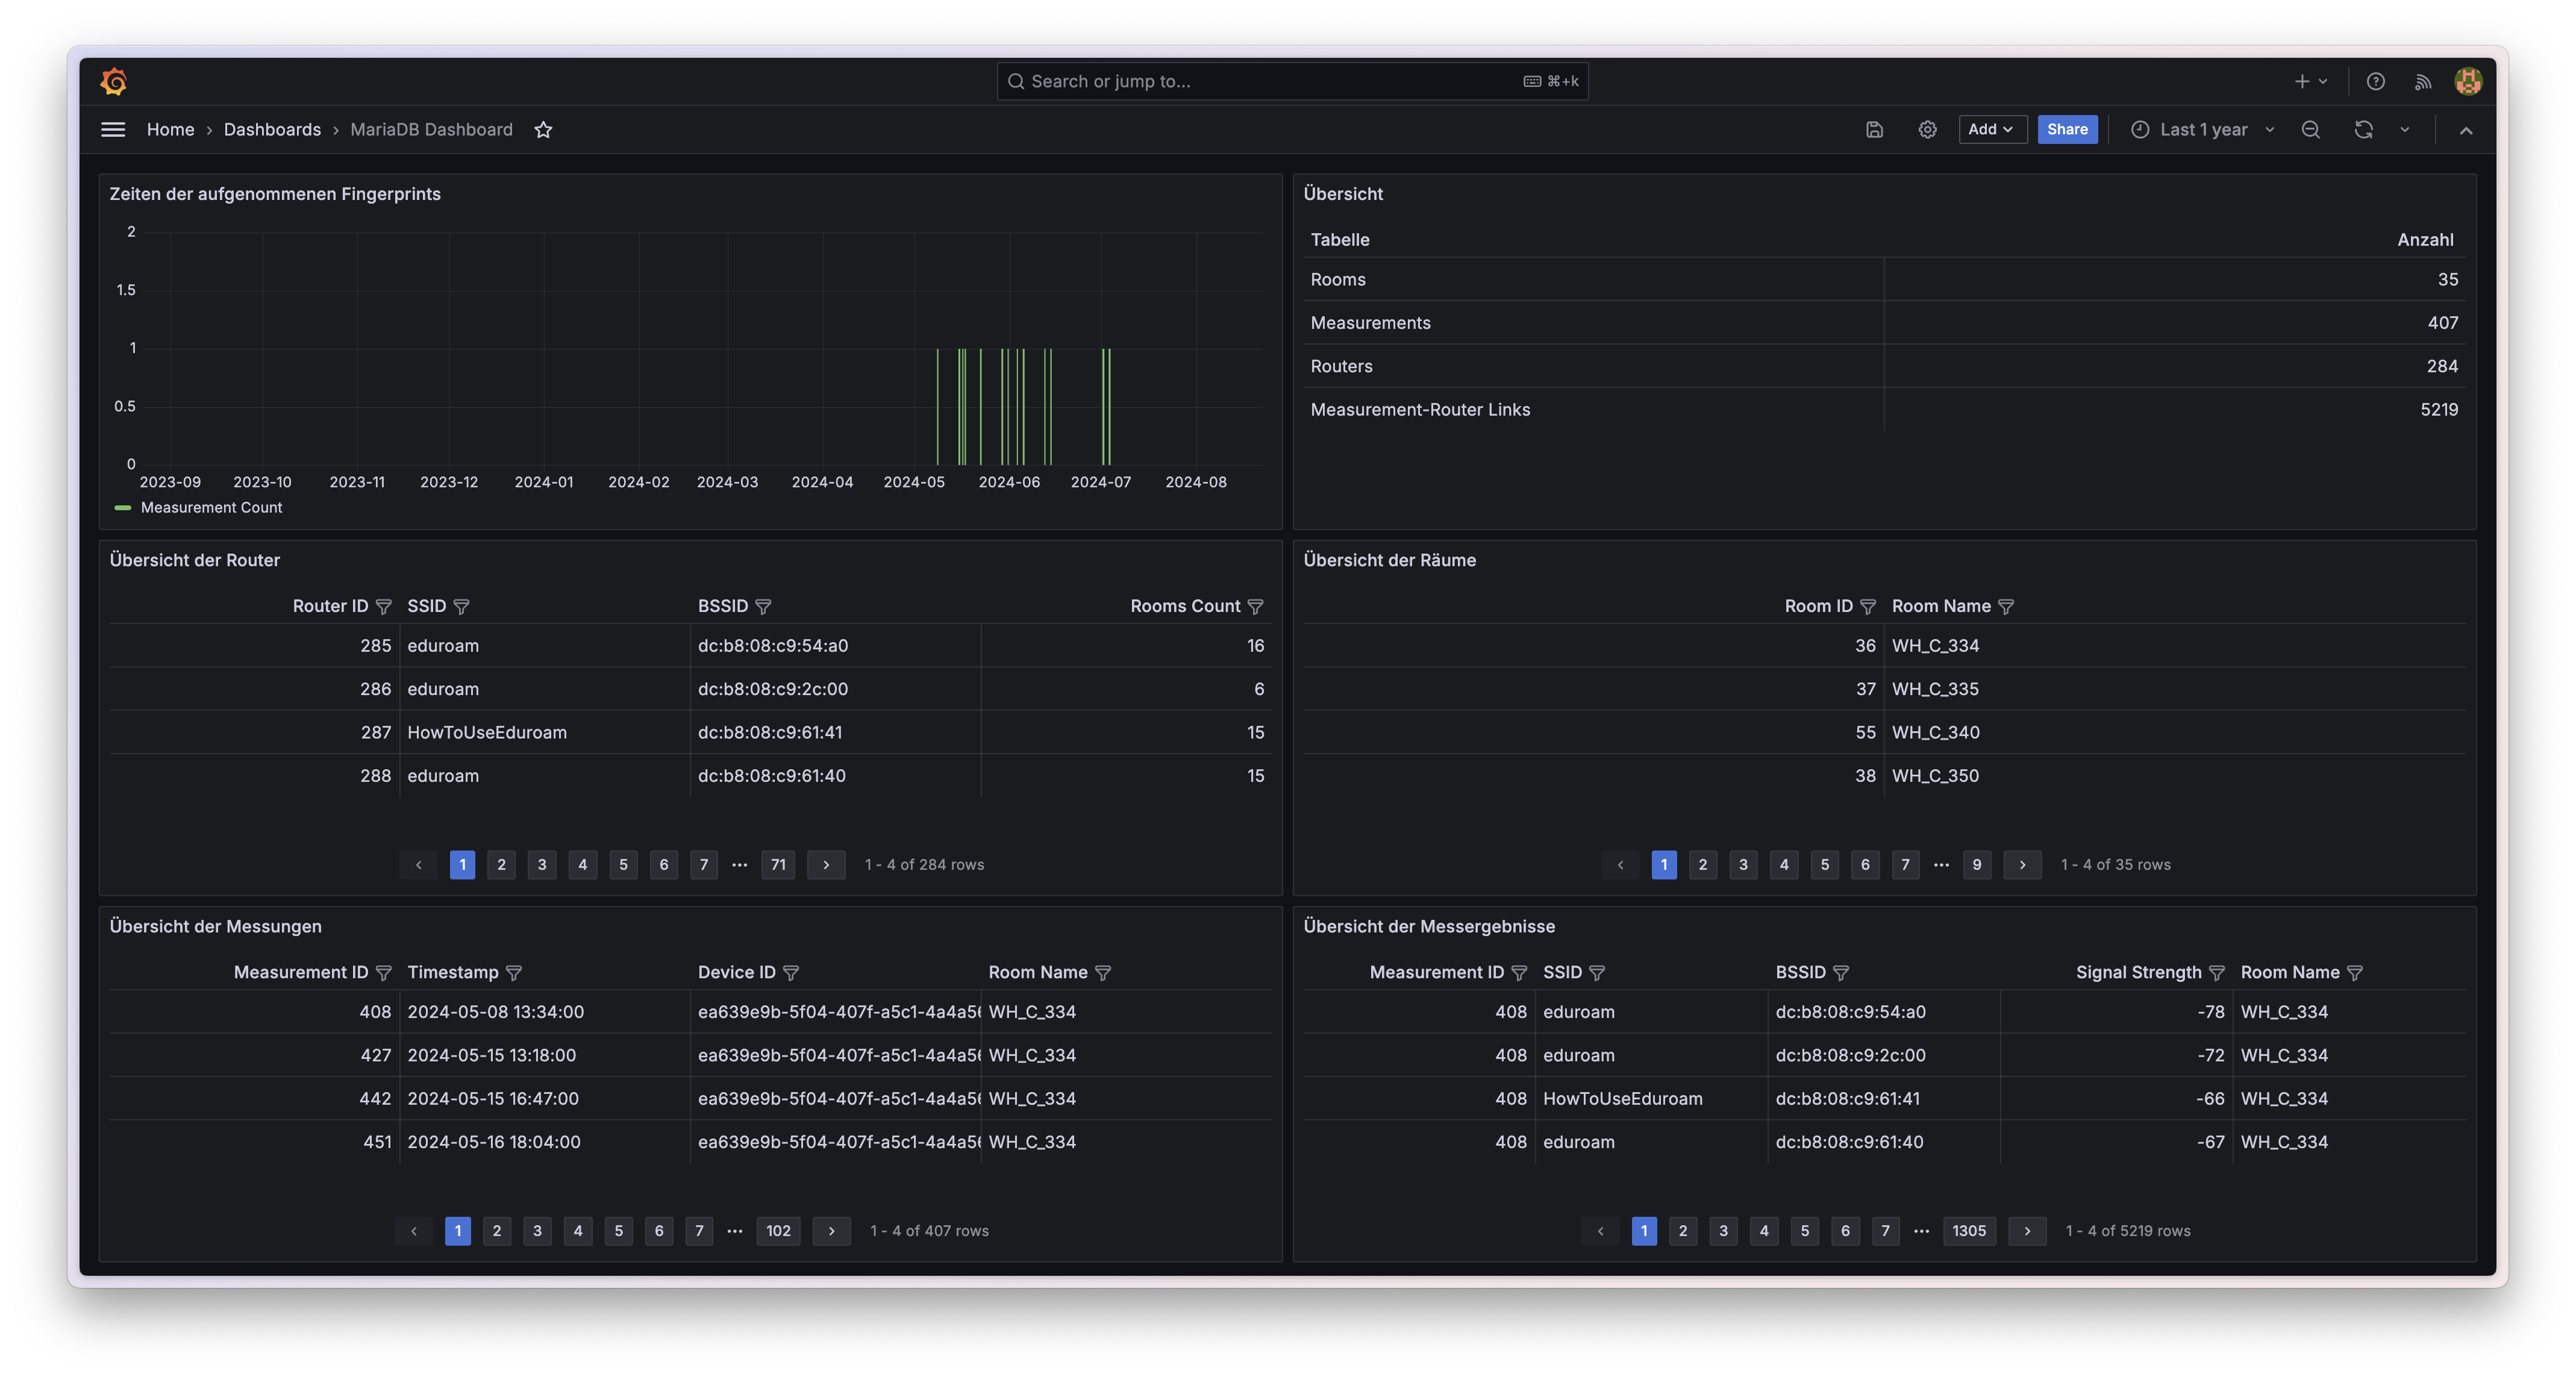
\includegraphics[width=0.8\textwidth]{images/grafana_fast_api_screenshot.png}
    \caption{Grafana Dashboard der \textit{FastAPI}}
    \label{fig:grafana_fast_api_screenshot}
\end{figure}

Für die Visualisierung der \textit{MariaDB} wurde ebenfalls ein \textit{Grafana}-Dashboard erstellt, welches eine Übersicht der Datenbank, die Inhalte der Tabellen und die Zeitpunkte darstellt, an denen die Messungen durchgeführt wurden (siehe Abbildung \ref{fig:grafana_maria_db_screenshot}). Die Dashboards können aus dem Netz der HTW über Adresse \texttt{http://141.45.212.246:3000} aufgerufen werden.

\begin{figure}[h]
    \centering
    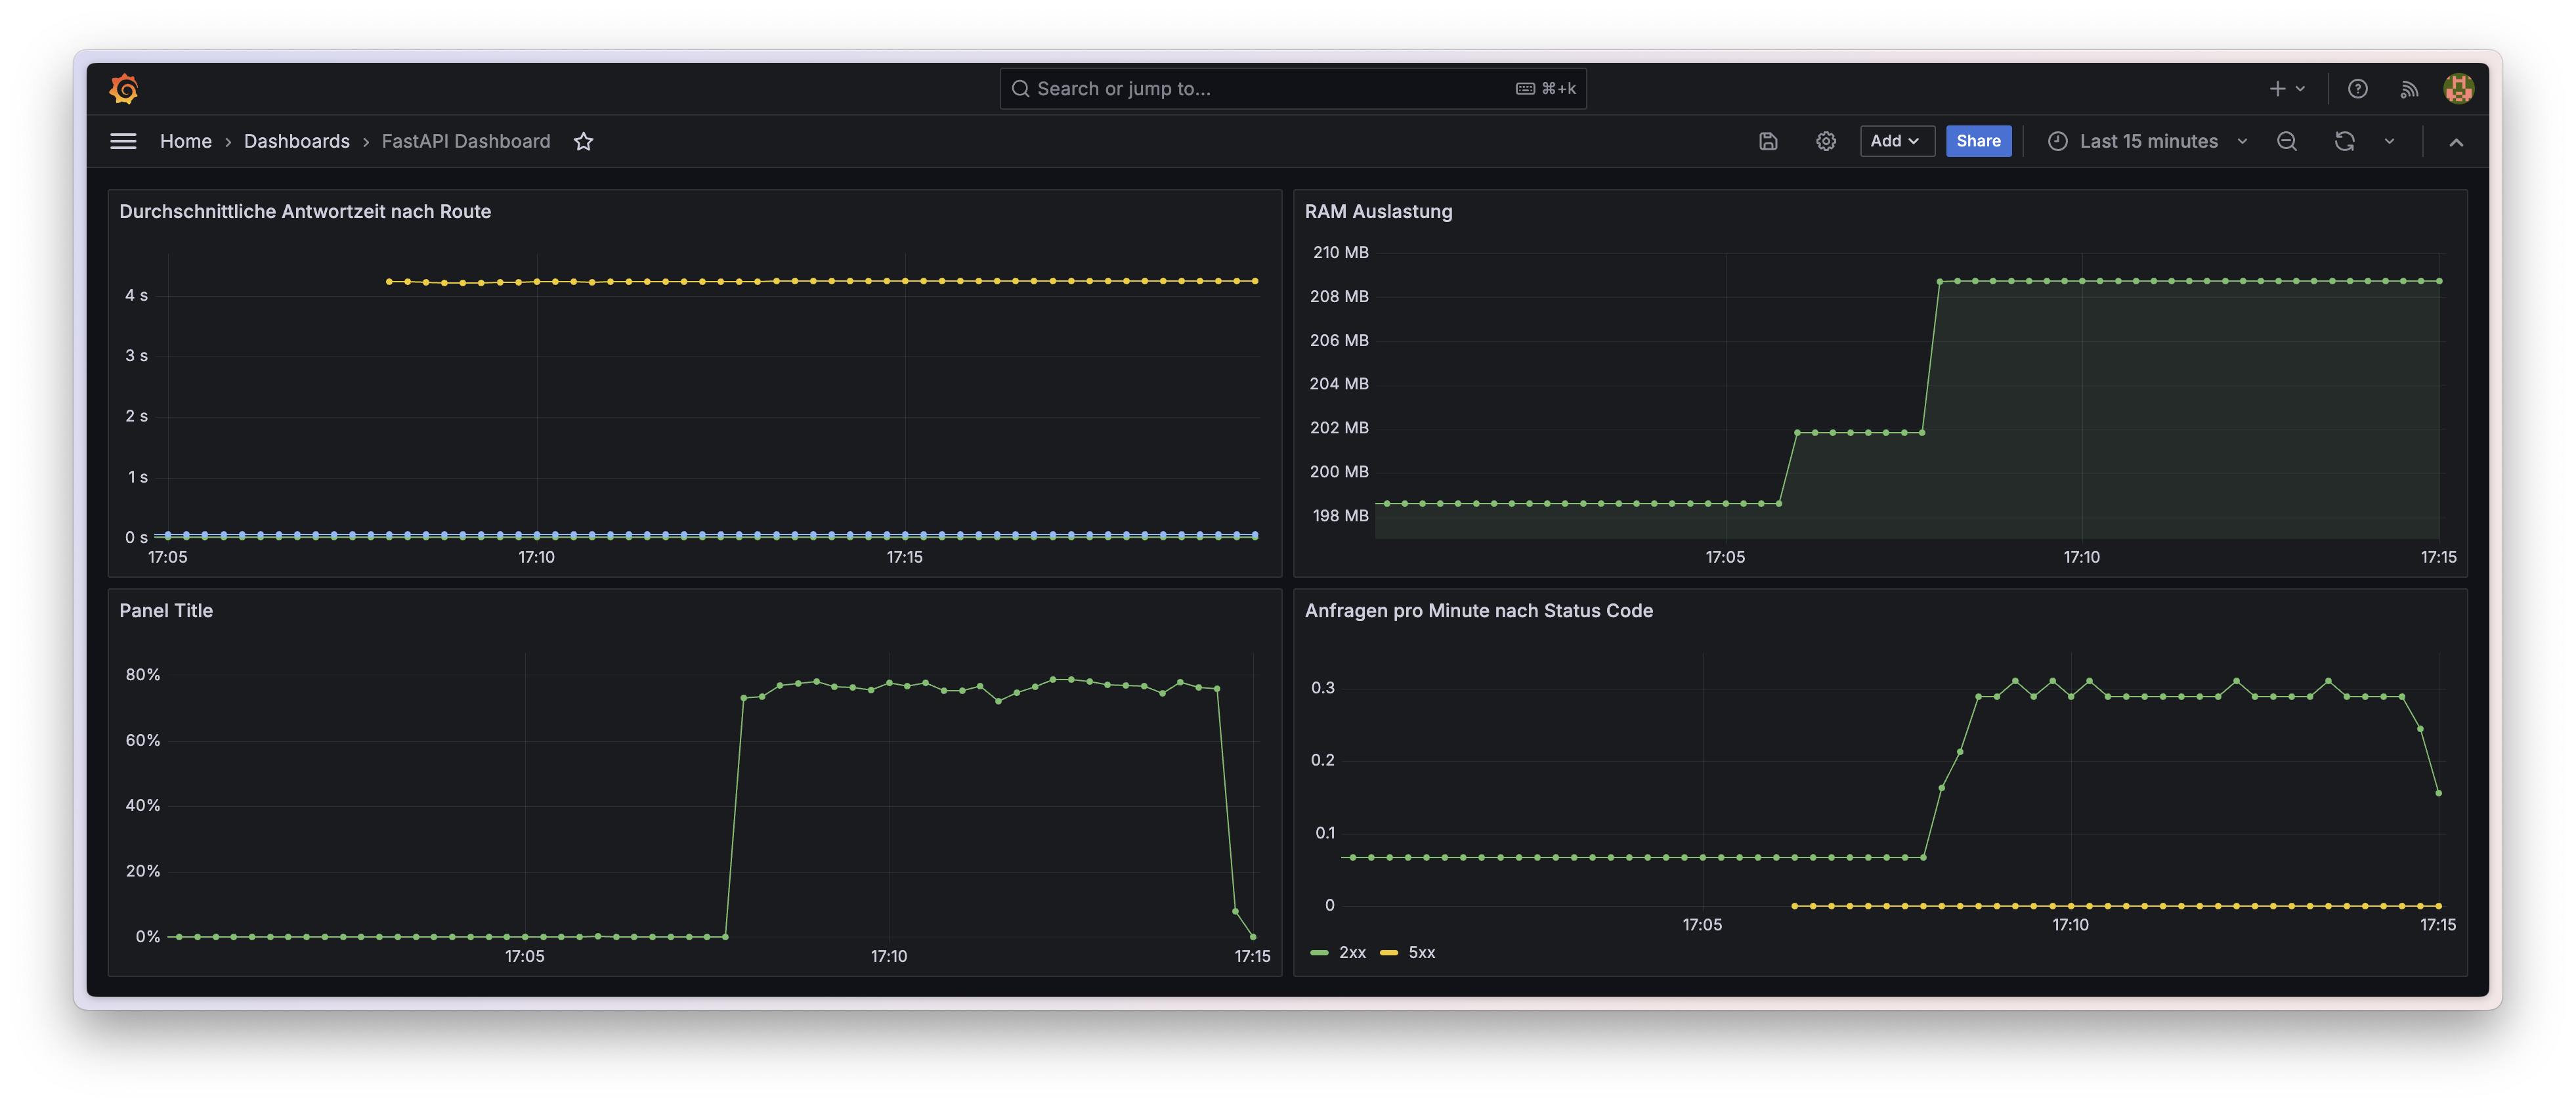
\includegraphics[width=0.8\textwidth]{images/grafana_maria_db_screenshot.png}
    \caption{Grafana Dashboard der \textit{MariaDB}}
    \label{fig:grafana_maria_db_screenshot}
\end{figure}

\section{Implementierung der \textit{BVG Detection} App}

Die Android App \textit{BVG Detection} (\url{https://github.com/OpenHistoricalDataMap/BVGDetection}) kann unteranderem dazu verwendet werden WiFi-Fingerprints von Orten zu speichern und die eigene Position anhand der bekannten WiFi-Fingerprints zu bestimmen. 

Die bisherige Implementierung wurde um die Funktionalität erweitert mehr als einen Fingerprint pro Raum aufzunehmen und die in der Offline Phase gemessenen Fingerprints mit anderen Geräten und der API auszutauschen. Zudem wurden die untersuchten Algortihmen aus dieser Arbeit für die Raumvorhersage implementiert.

\subsection{Wiederinbetriebnahme der App}

In der bisherigen Implementierung konnte die App zum Zeitpunkt dieser Arbeit nicht mehr kompiliert werden. Dies lag daran, dass das verwendete Build-Tool \textit{Gradle} veraltet war und in der aktuellen Version von \textit{Android Studio (Koala | 2024.1.1)} nicht mehr unterstützt wurde. Damit die App wieder kompiliert werden konnte, wurde \textit{Gradle} von der Version \texttt{2.3.3} auf die Version \texttt{8.3.2} aktualisiert.\mycitefoot{androidAndroidGradle} % https://developer.android.com/build/releases/gradle-plugin

Zudem wurden die verwendeten \textit{Android Support Libraries}, welche veraltet sind und für die UI-Komponenten und die Abwärtskompatibilität zuständig sind, durch \textit{AndroidX} ersetzt.\mycitefoot{androidSupportLibrary} % https://developer.android.com/topic/libraries/support-library/packages

Durch diese Änderungen kann die \textit{BVG Detection}-App wieder kompiliert werden und wird auf allen Android Geräten mit Android 9.0 (Pie) oder höher unterstützt.

\subsection{Datenspeicherung und Aufnahme der WiFi-Fingerprints}

In der bisherigen Implementierung war bereits eine \textit{SQLite}-Datenbank vorhanden. Diese wurde durch die in Kapitel \ref{datenbank} erläuterte Datenbank ersetzt. Über den Menüpunkt \textit{Ort/Fingerprint aufnehmen} (siehe Abbildung \ref{fig:bvg_detection_capture}) kann ein neuer Raum inklusive Fingerprint hinzugefügt werden bzw. für einen bereits vorhandenen Raum ein neuer Fingerprint aufgenommen werden. Bei der Aufnahme eines neuen Fingerprints muss der Raumname angegeben werden, damit der Fingerprint diesem Raum zugeordnet werden kann. Sollte es bereits eine Messung von diesem Raum geben, kann dieser aus einem Dropdown Menü ausgewählt werden. Optional kann auch eine Beschreibung des Raums sowie ein Foto des Raums hinzugefügt werden. Für die Aufnahme der Fingerprints nutzt die App den Android \texttt{WiFiManager}. Seit der Android Version 9 ist die Anazhl der WiFi-Scans auf vier Scans innerhalb von 2 Minuten limitiert. Aus diesem Grund wird bei der Aufnahme eines neuen Fingerprints alle 30 Sekunden, sofern mehrere Fingerprints aufgenommen werden sollen, ein Scan durchgeführt.\mycitefoot{androidWiFiScanning}

\begin{figure}[h]
    \centering
    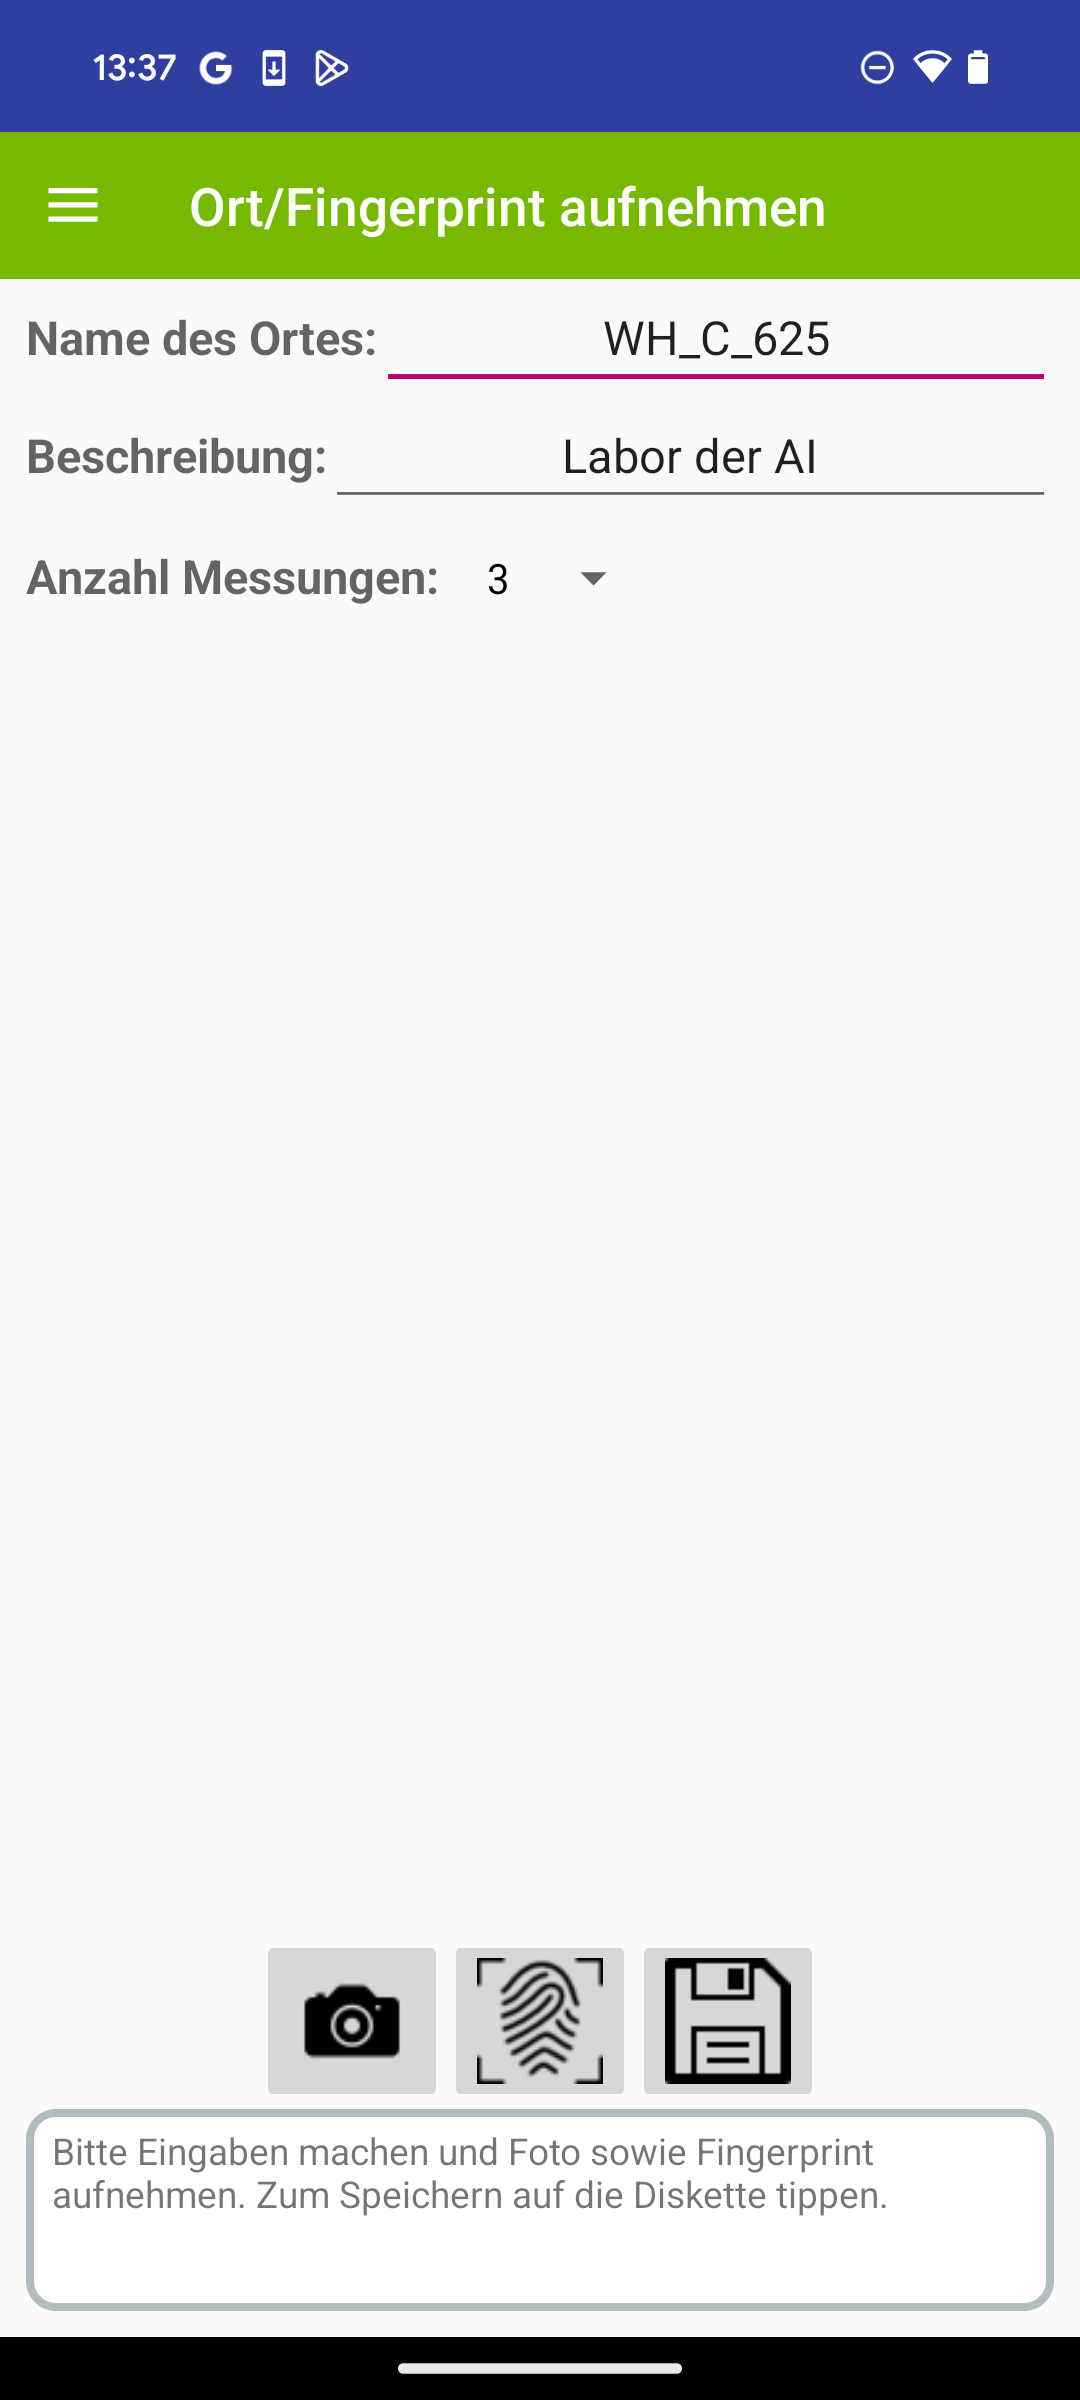
\includegraphics[width=0.3\textwidth]{images/screenshots/capture.png}
    \caption{Menüpunkt \textit{Ort/Fingerprint aufnehmen} der \textit{BVG Detection}-App}
    \label{fig:bvg_detection_capture}
\end{figure}

Unter dem Menüpunkt \textit{Fingerprints verwalten} (siehe Abbildung \ref{fig:bild1}) können alle Räume inklusive Messungen der Messungen (siehe Abbildung \ref{fig:bild2}) und den darin enthaltenen Access Points (siehe Abbildung \ref{fig:fingerprints-verwalten}) angezeigt werden.

\begin{figure}[h!]
    \centering
    \begin{subfigure}[b]{0.3\textwidth}
        \centering
        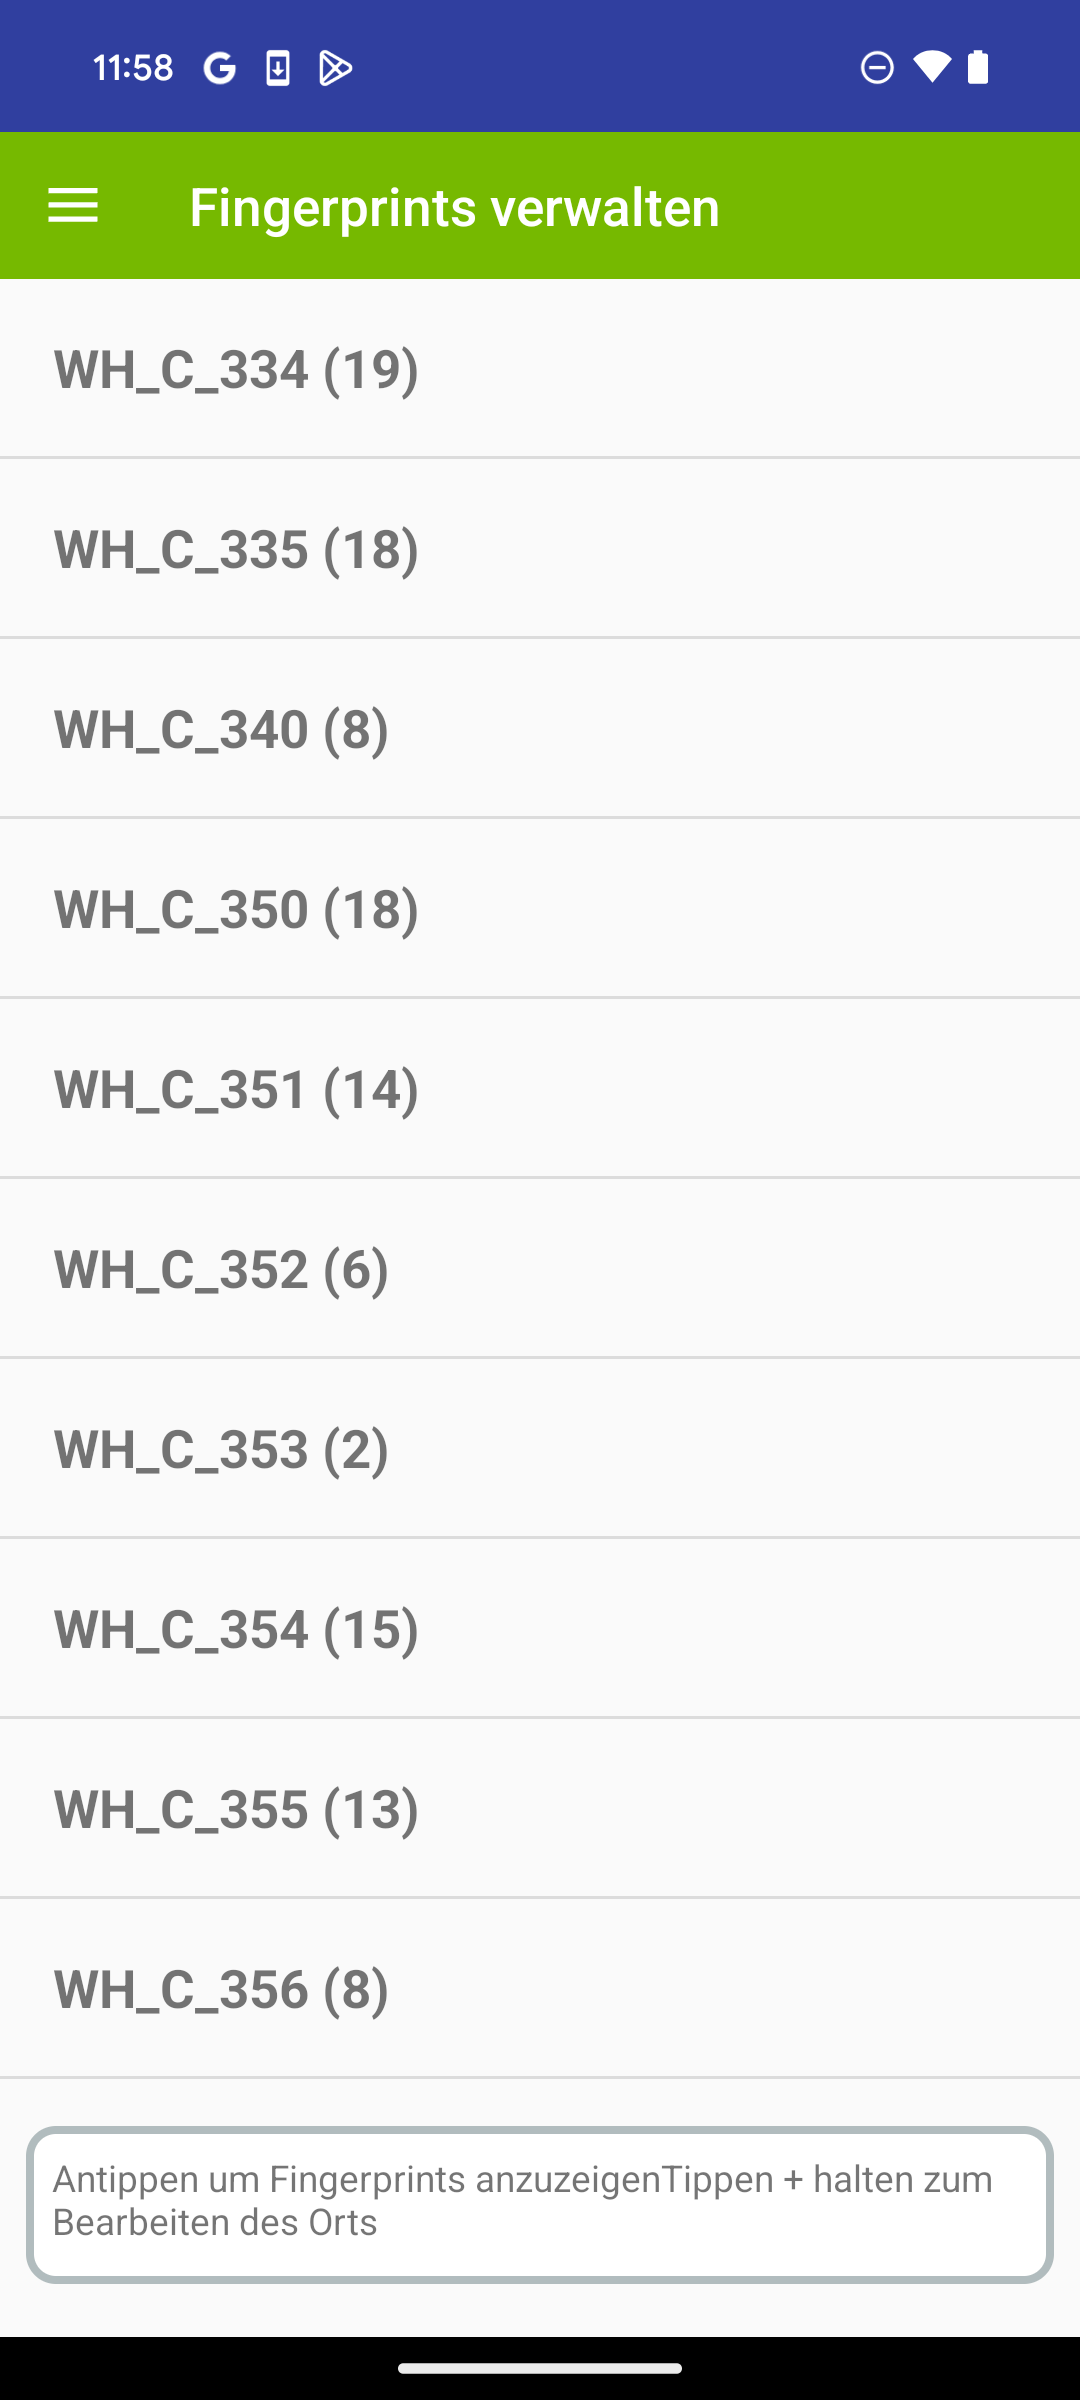
\includegraphics[width=\textwidth]{images/screenshots/all_rooms.png}
        \caption{Übersicht der gespeicherten Orte}
        \label{fig:bild1}
    \end{subfigure}
    \hfill
    \begin{subfigure}[b]{0.3\textwidth}
        \centering
        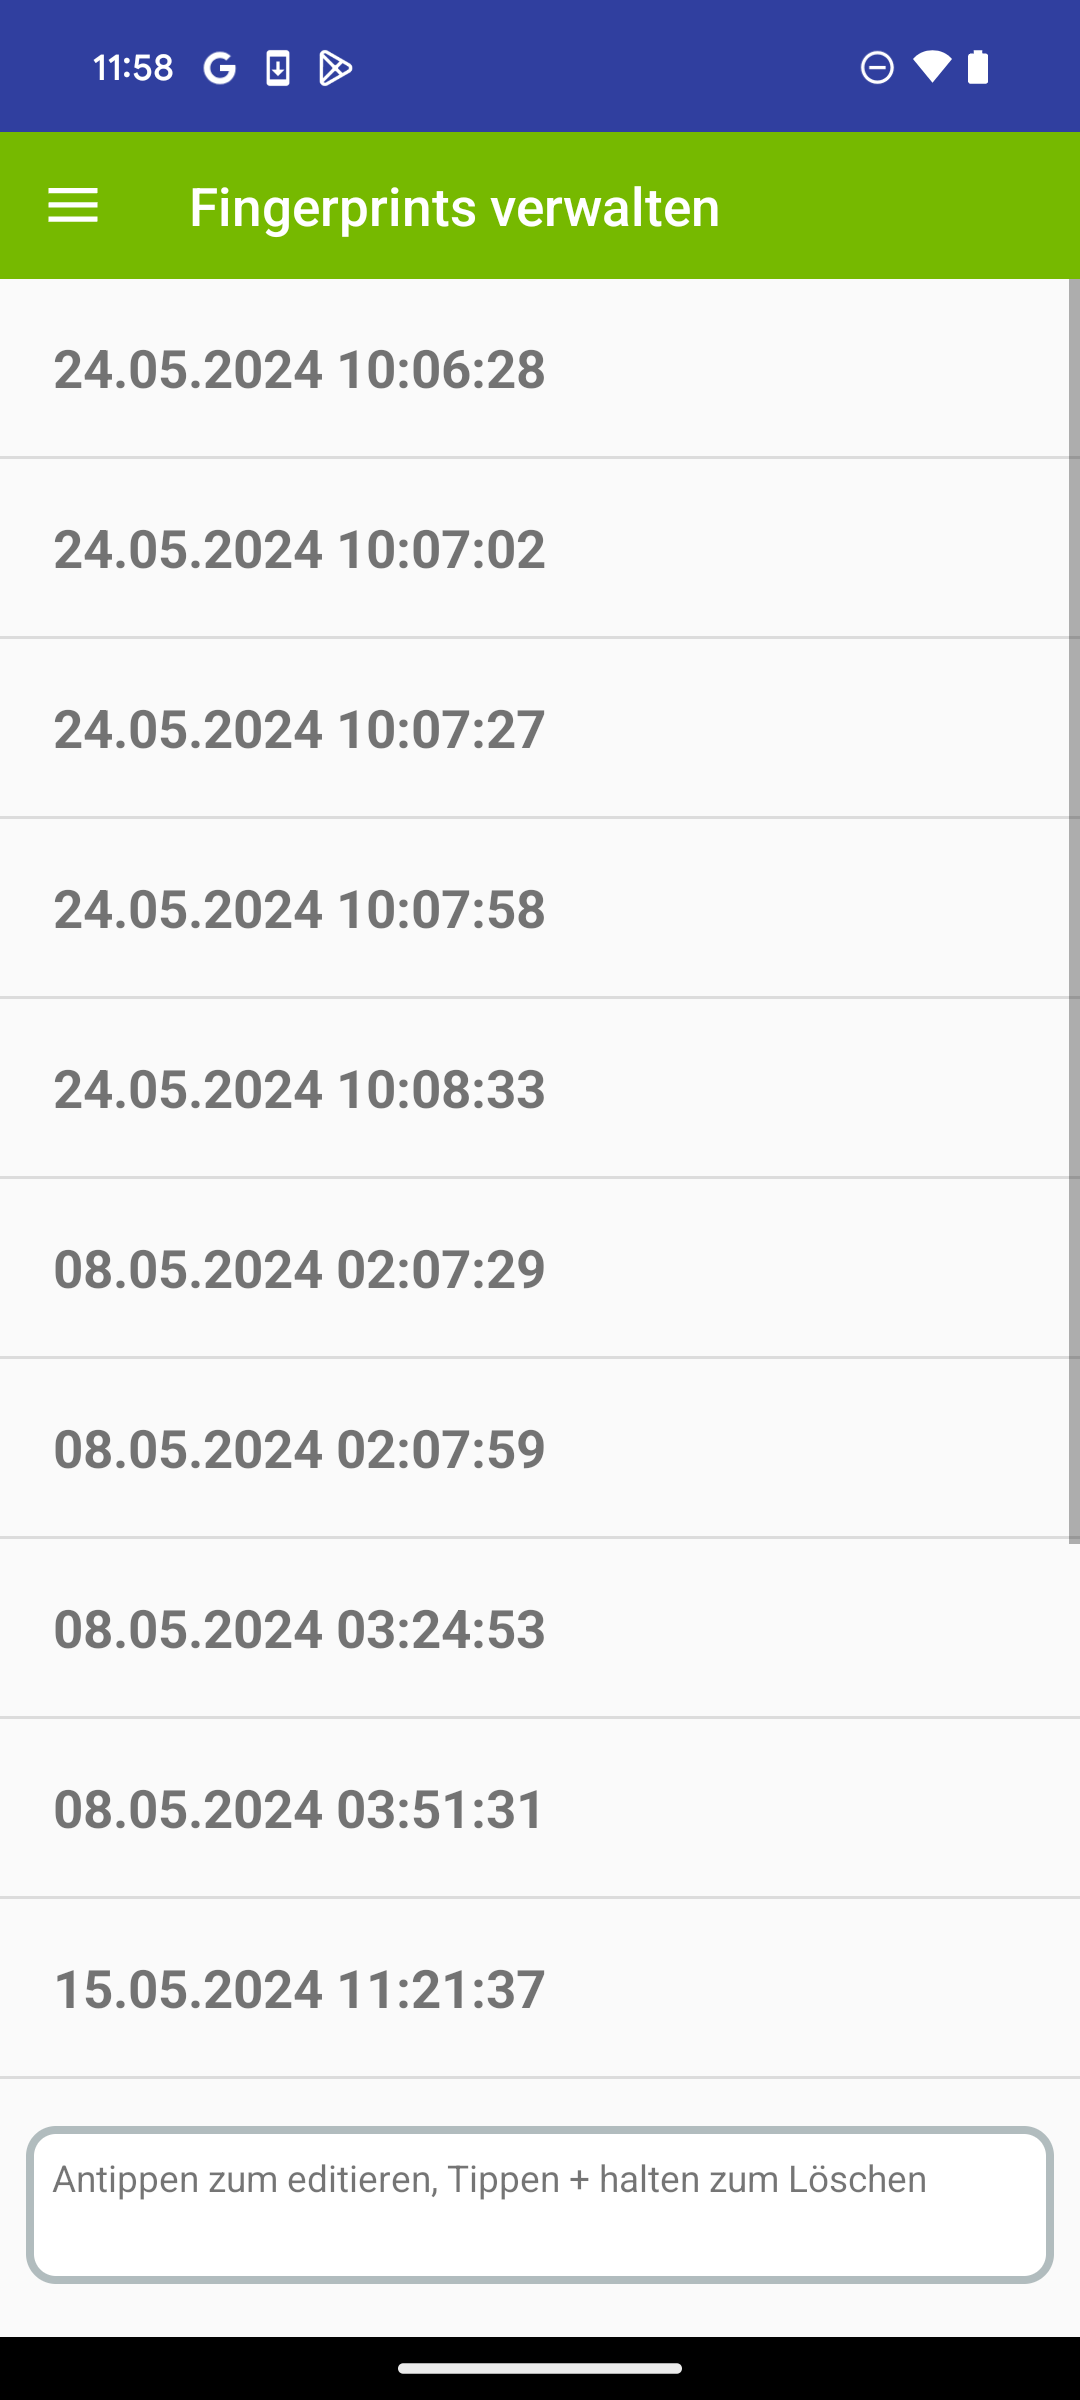
\includegraphics[width=\textwidth]{images/screenshots/all_measurements.png}
        \caption{Übersicht der Messungen eines Raumes}
        \label{fig:bild2}
    \end{subfigure}
    \hfill
    \begin{subfigure}[b]{0.3\textwidth}
        \centering
        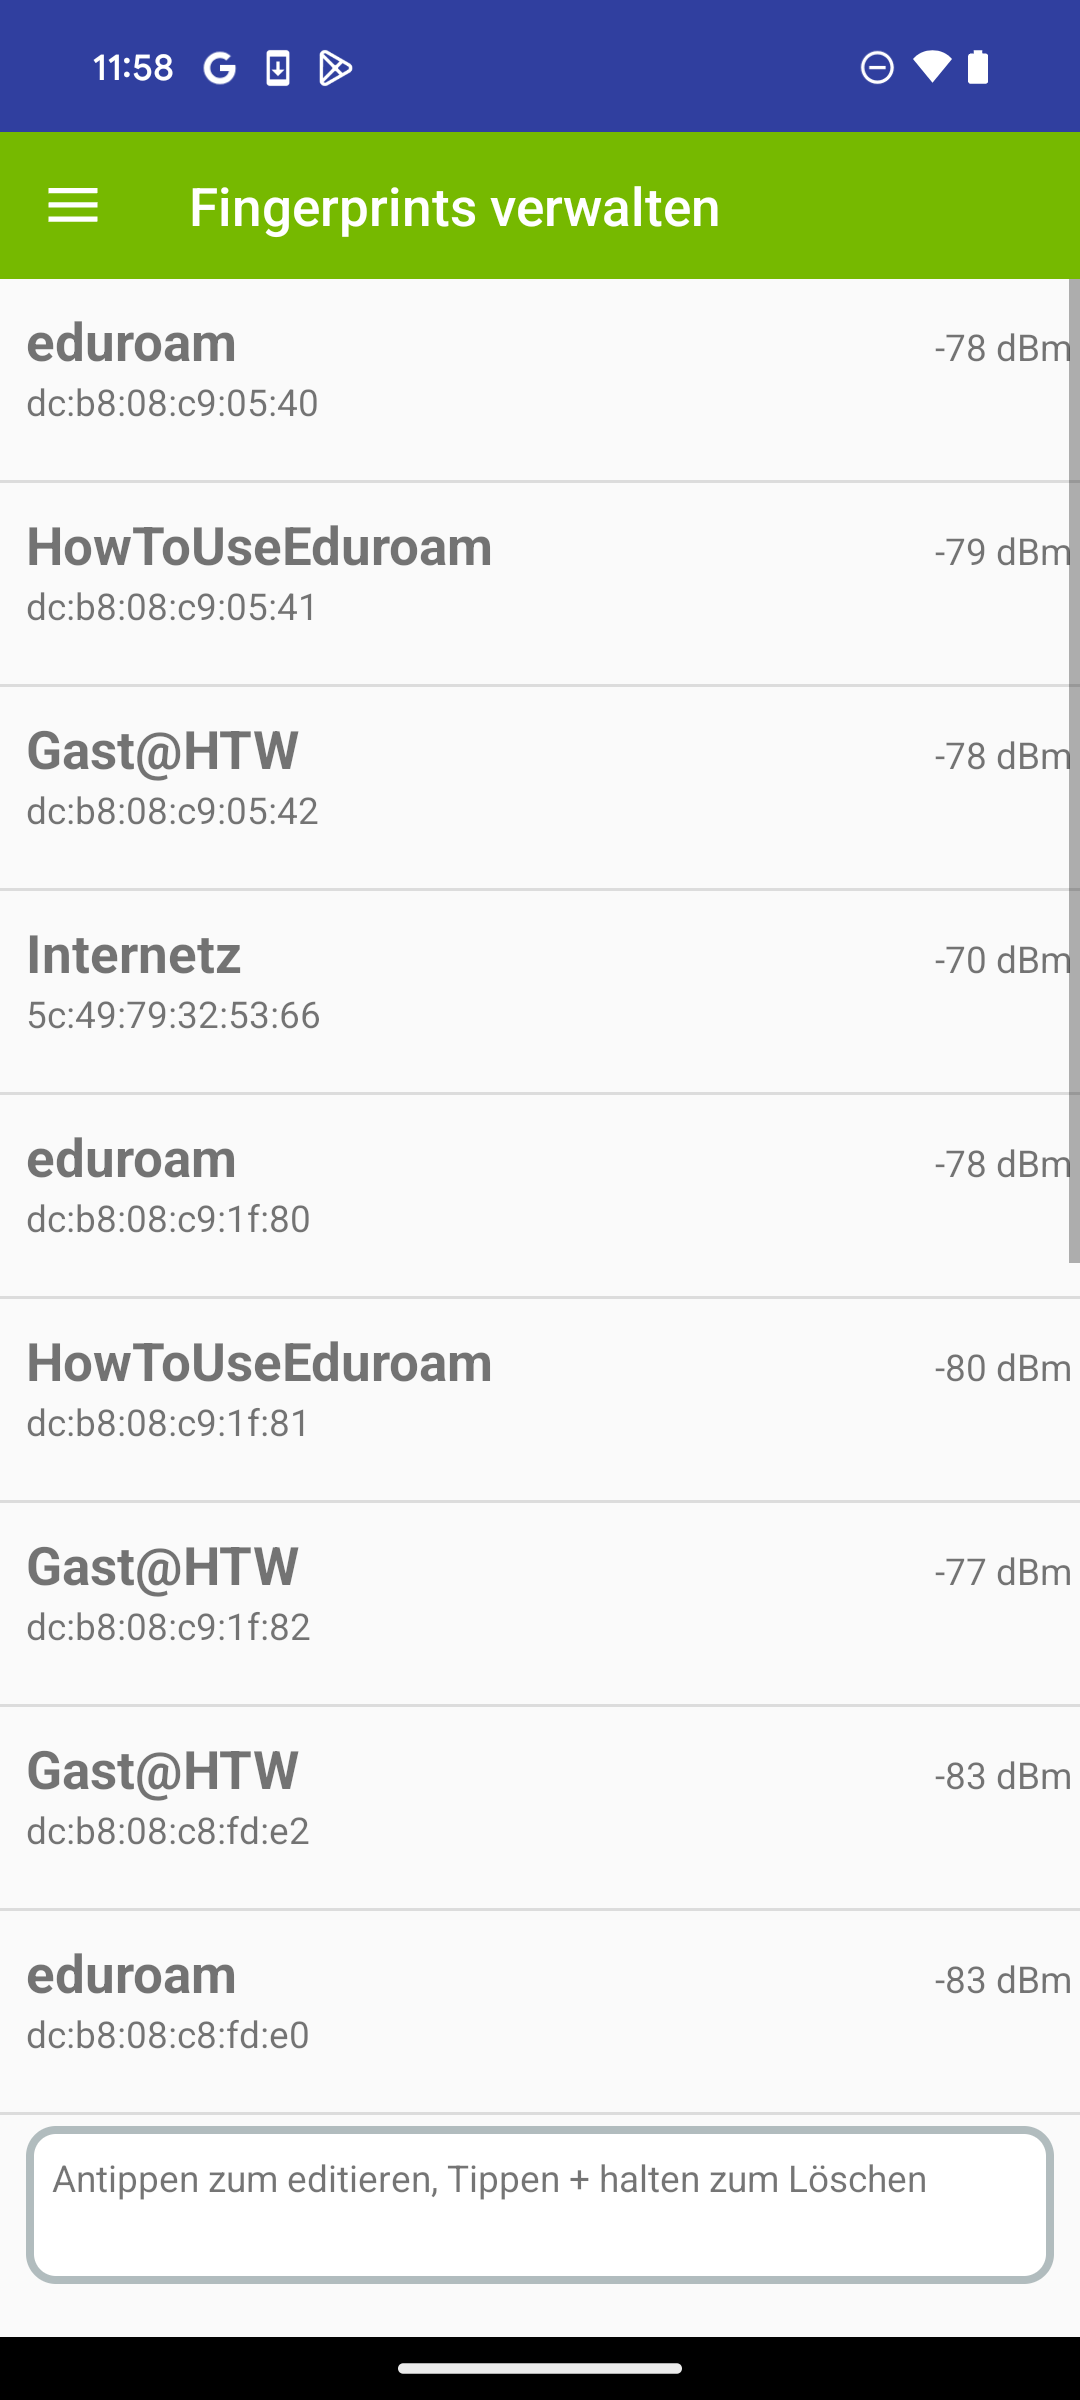
\includegraphics[width=\textwidth]{images/screenshots/fingerprint.png}
        \caption{Übersicht der Access Points einer Messung}
        \label{fig:bild3}
    \end{subfigure}
    \caption{Menüpunkt \textit{Fingerprints verwalten} der \textit{BVG Detection}-App}
    \label{fig:fingerprints-verwalten}
\end{figure}

Die kompilierte Version der App ist in dem \textit{GitLab}-Repository dieser Arbeit in dem Unterordner \texttt{bvg-detection-app} zu finden und in dem \textit{GitHub}-Repository der \textit{BVG Detection} App (\url{https://github.com/OpenHistoricalDataMap/BVGDetection}) auf dem Branch \texttt{v2}.

\subsection{Austausch der Daten}

Für den Austausch der Daten wurde der Menüpunkt \textit{Datenbank teilen} (siehe Abbildung \ref{fig:bvg_detection_share_database}) hinzugefügt. Unter diesem Menüpunkt können die gespeicherter Fingerprints per Bluetooth an andere Geräte gesendet werden bzw. von anderen Geräten empfangen werden und an die API aus Kapitel \ref{api} gesendet bzw. von dieser empfangen werden. 

Damit die Daten über Bluetooth ausgetauscht werden können, müssen beide Geräte eine Blue\-tooth-Verbindung eingehen. Dazu muss eins der beiden Geräte einen \texttt{BluetoothSocket} und das andere Gerät einen \texttt{BluetoothServerSocket} öffnen. Dies geschieht über die beiden Buttons \textit{Listen} und \textit{List Devices}. Im Anschluss werden alle sichtabren Geräte in einer Liste angezeigt und das entsprechende Gerät kann ausgewählt werden. Nachdem beide Geräte eine Bluetooth Verbindung aufgebaut haben, wird das in der App in dem Statustextfeld angezeit und über den Button \textit{Send} kann der Transfer der Daten gestartet werden.

Die zu übertragenden Messdaten werden aus der \textit{SQLite}-Datenbank des sendenden Geräts in einem \textit{JSON}-Array gesammelt. Anschließend wird dieses Array durchlaufen und jeder Eintrag in ein Byte-Array umgewandelt, welches dann über die Bluetooth Verbindung an den Empfänger gesendet werden kann.

Um die Struktur der gesendeten Daten zu kennzeichnen und die Nachrichten korrekt zu trennen, wird zwischen den einzelnen Messungen das Trennzeichen (\texttt{MESSAGE\_SPLIT \allowbreak = \allowbreak \grqq{}\_NEW\_MESSAGE\_\allowbreak \grqq{}}) eingefügt und am Ende der gesamten Übertragung wird das Endzeichen (\texttt{MESSAGE\_END \allowbreak = \allowbreak \grqq{}\_MESSAGE\_END\_\allowbreak \grqq{}}) gesendet. Dadurch wird der Empfänger darüber informiert, dass die Übertragung abgeschlossen ist. Der Empfänger sammelt die eingehenden Daten, bis das Endzeichen erkannt wird. Anschließend werden die gesammelten Daten wieder in ein \textit{JSON}-Array konvertiert und in der \textit{SQLite}-Datenbank des Empfängers gespeichert.

Für den Austausch der Daten mit der API aus Kapitel \ref{api} muss sich das Smartphone in dem Netzwerk der HTW Berlin befinden. Wenn das der Fall ist kann über den Button \textit{Send to API} die Übertragung der Messungen an die API gestartet werden. Über den Button \textit{Receive from API} werden alle Fingerprints die in der \textit{MariaDB} auf dem Server gespeichert sind empfangen und lokal gespeichert werden 

\begin{figure}[h]
    \centering
    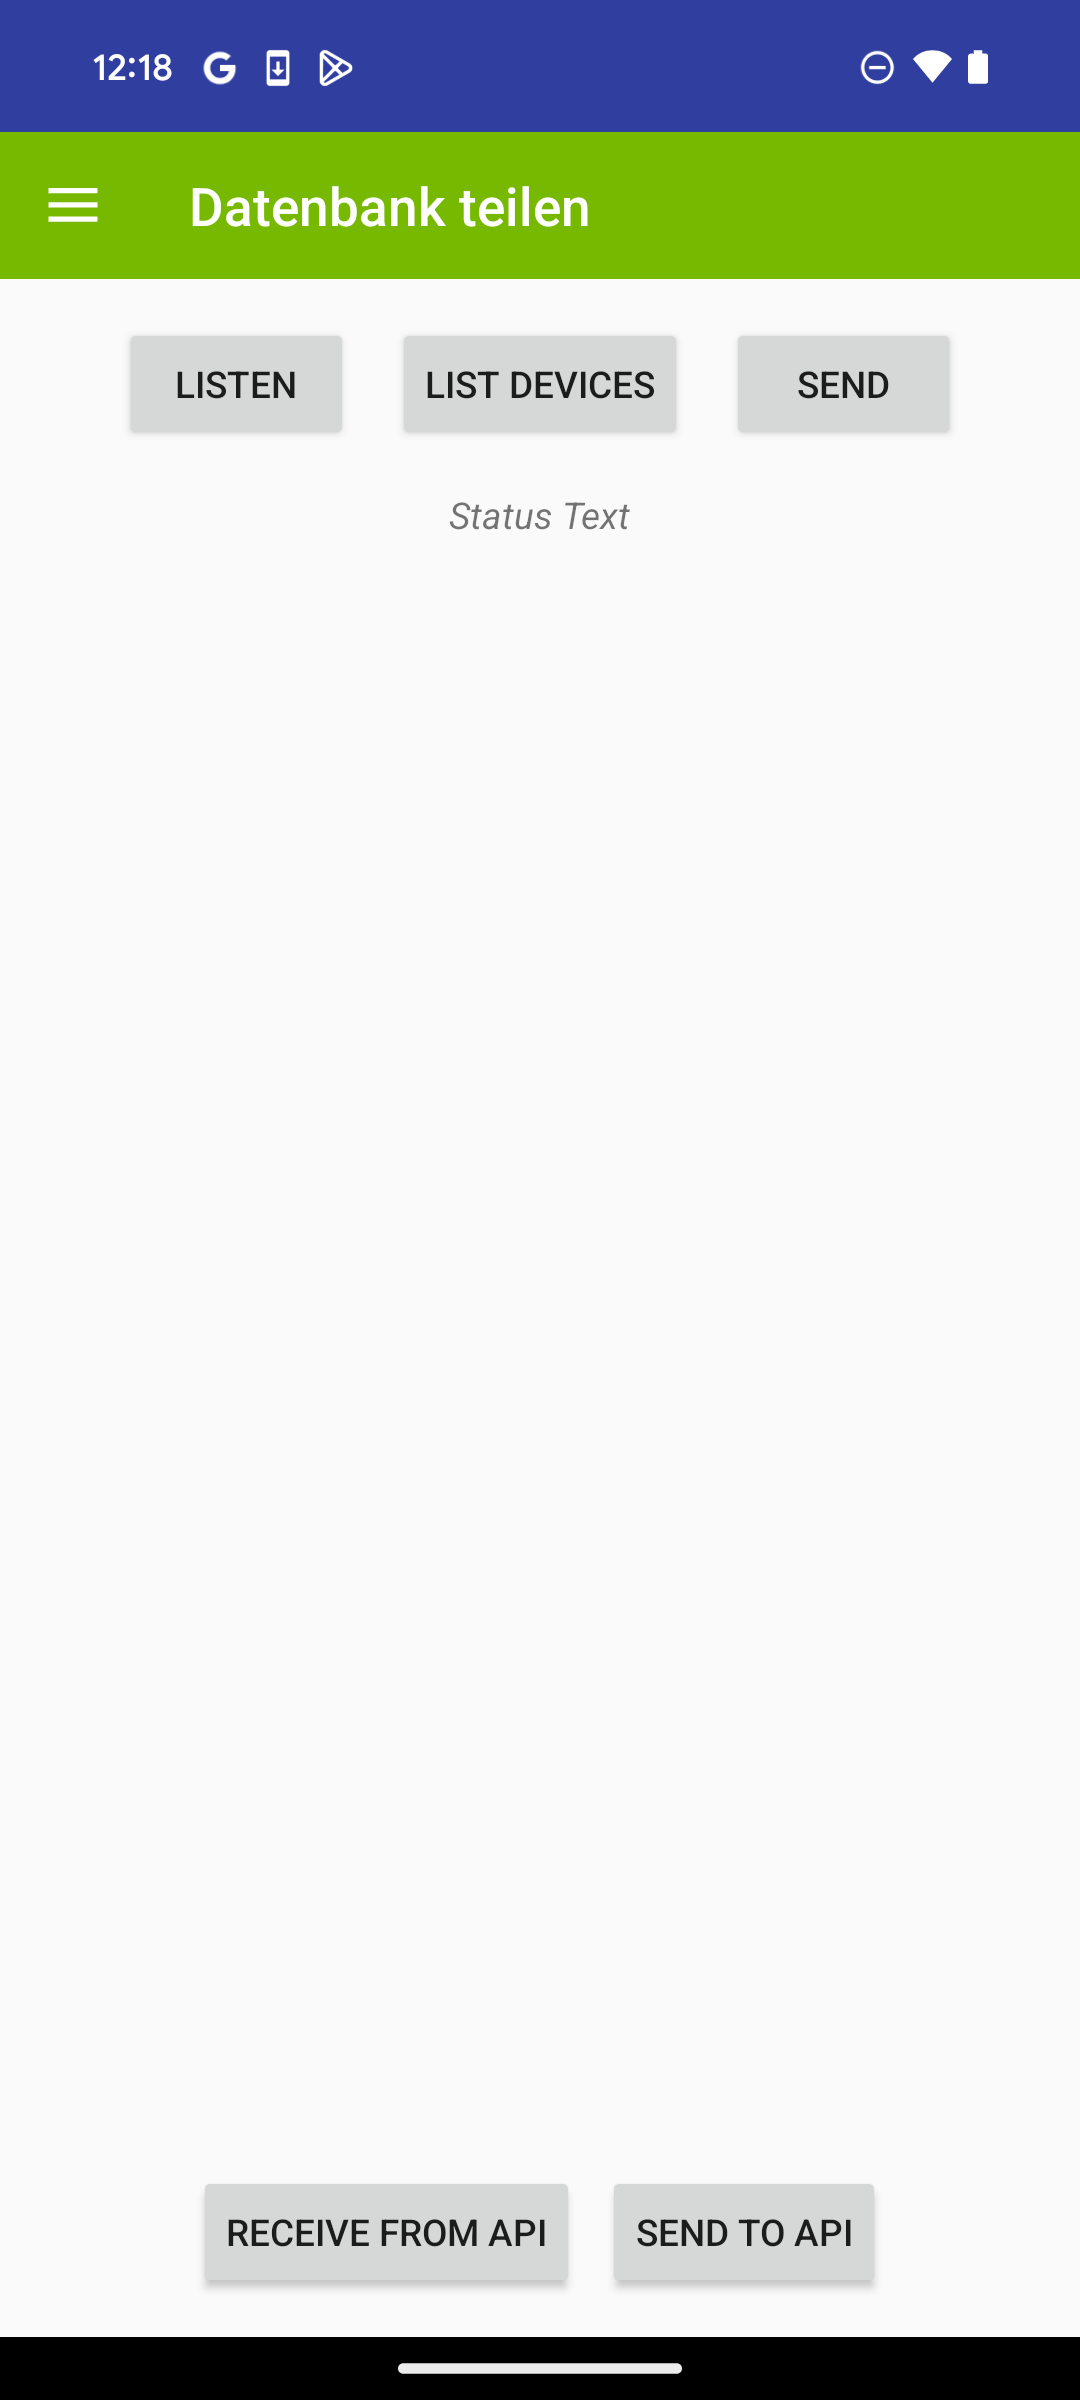
\includegraphics[width=0.3\textwidth]{images/screenshots/share_database.png}
    \caption{Menüpunkt \textit{Datenbank teilen} der \textit{BVG Detection}-App}
    \label{fig:bvg_detection_share_database}
\end{figure}

Da die API auf einem HTTP-Server läuft und kein SSL Zertifikat hat, muss der Zugriff explizit erlaubt werden, indem die IP-Adresse des Servers in der Netzwerkkonfiguration der App eingetragen wird. Sollte sich die IP-Adresse des Servers ändern, muss diese manuell im Quellcode der App geändert werden.

\begin{lstlisting}[caption={Netzwerkkonfiguration der App}]
<?xml version="1.0" encoding="utf-8"?>
<network-security-config>
    <domain-config cleartextTrafficPermitted="true">
    <domain includeSubdomains="true">141.45.212.246</domain>
    </domain-config>
</network-security-config>    
\end{lstlisting}

\subsection{Ortung von Räumen}

Die Ortung kann über den Menüpunkt \textit{Standort ermitteln} (siehe Abbildung \ref{fig:app-localize-1}) gestartet werden und wird lokal auf dem Gerät ausgeführt. Dazu wurden die in dieser Arbeit untersuchten Algorithmen (\gls{knn}, \gls{svm} und Random Forest), die dazugehörigen Parameter und die Datenaufbereitungsschritte (siehe Kapitel \ref{datenaufbereitung}) implementiert. Aus dem Grund, dass für die Algorithmen in der API die Python Bibliothek \textit{scikit-learn} verwendet wurde und diese nicht unter Android verwendet werden kann, wurden die Algorithmen in Java nachimplementiert. 

Der \gls{knn} und Random Forest Algorithmus wurden nach den Vorlagen von \textit{Kenzo Takahashi} und \textit{Florian Zyprian}, in welchen die Algorithmen von \textit{scikit-learn} nachimplementiert wurden, implementiert\mycitefoot{kenzotakahashiKNearestNeighbor}\textsuperscript{,}\mycitefoot{konfuzioRandomForest}. Für die Implementierung des \gls{svm} Algorithmus wurde die Bibliothek \textit{AndroidLibSvm} (\url{https://github.com/yctung/AndroidLibSVM}), welche eine Open-Source Implementierung der \textit{LIBSVM} Bibliothek (\url{https://www.csie.ntu.edu.tw/~cjlin/libsvm/}) ist, verwendet.

Die Algorithmen inklusive Parameter und die verschiedenen Methoden zur Aufbereitung der Daten können in den Einstellungen (siehe Abbildungen \ref{fig:app-localize-2} und \ref{fig:app-localize-3}) ausgewählt werden und werden bei der Ortung (siehe Abbildung \ref{fig:app-localize-1}) angezeigt.

\begin{figure}[h!]
    \centering
    \begin{subfigure}[b]{0.3\textwidth}
        \centering
        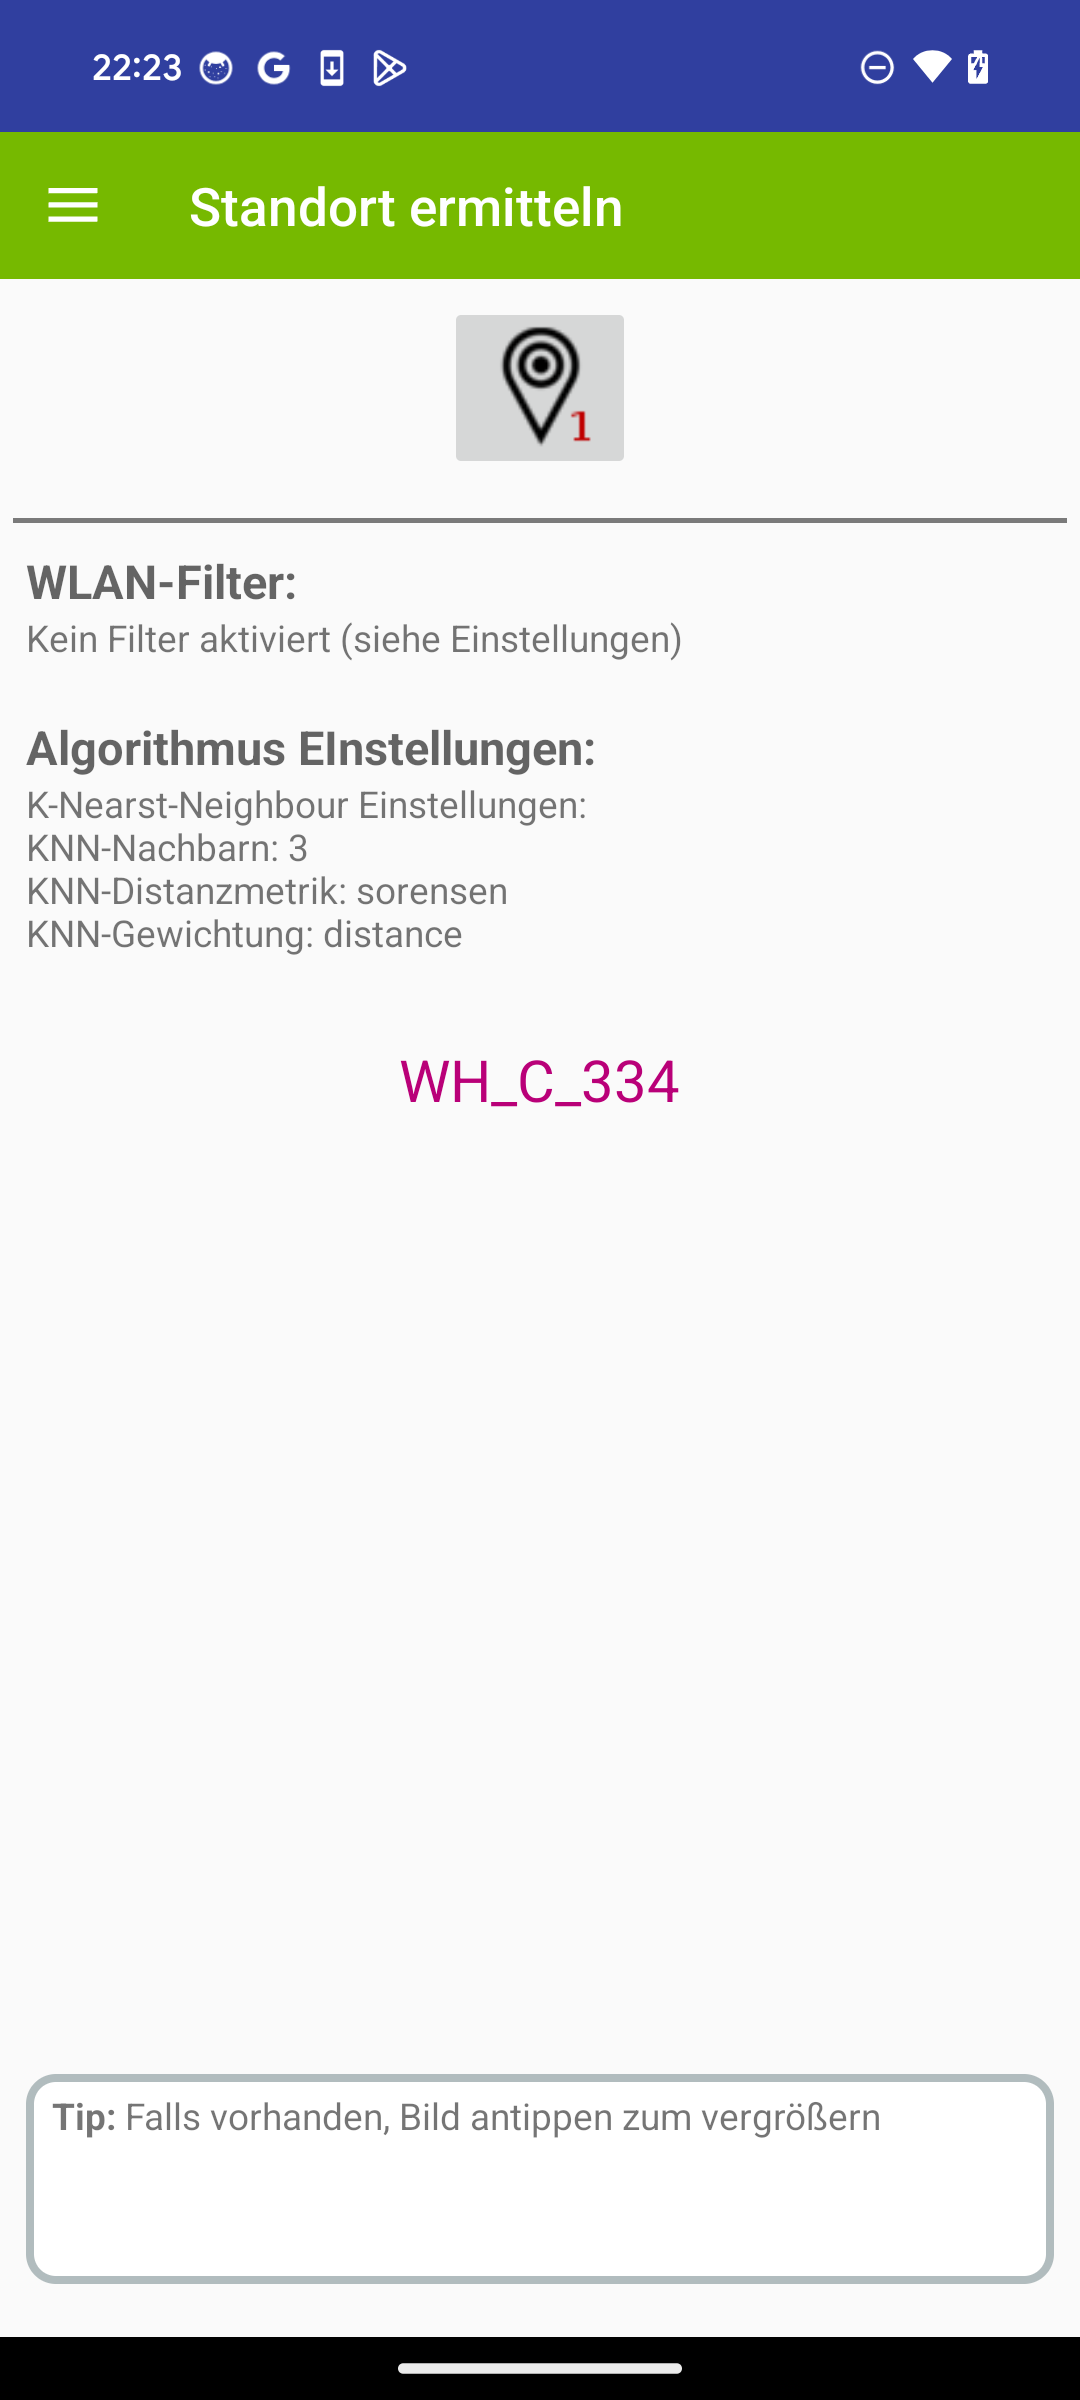
\includegraphics[width=\textwidth]{images/screenshots/localize.png}
        \caption{Menüpunkt \textit{Standort ermitteln}}
        \label{fig:app-localize-1}
    \end{subfigure}
    \hfill
    \begin{subfigure}[b]{0.3\textwidth}
        \centering
        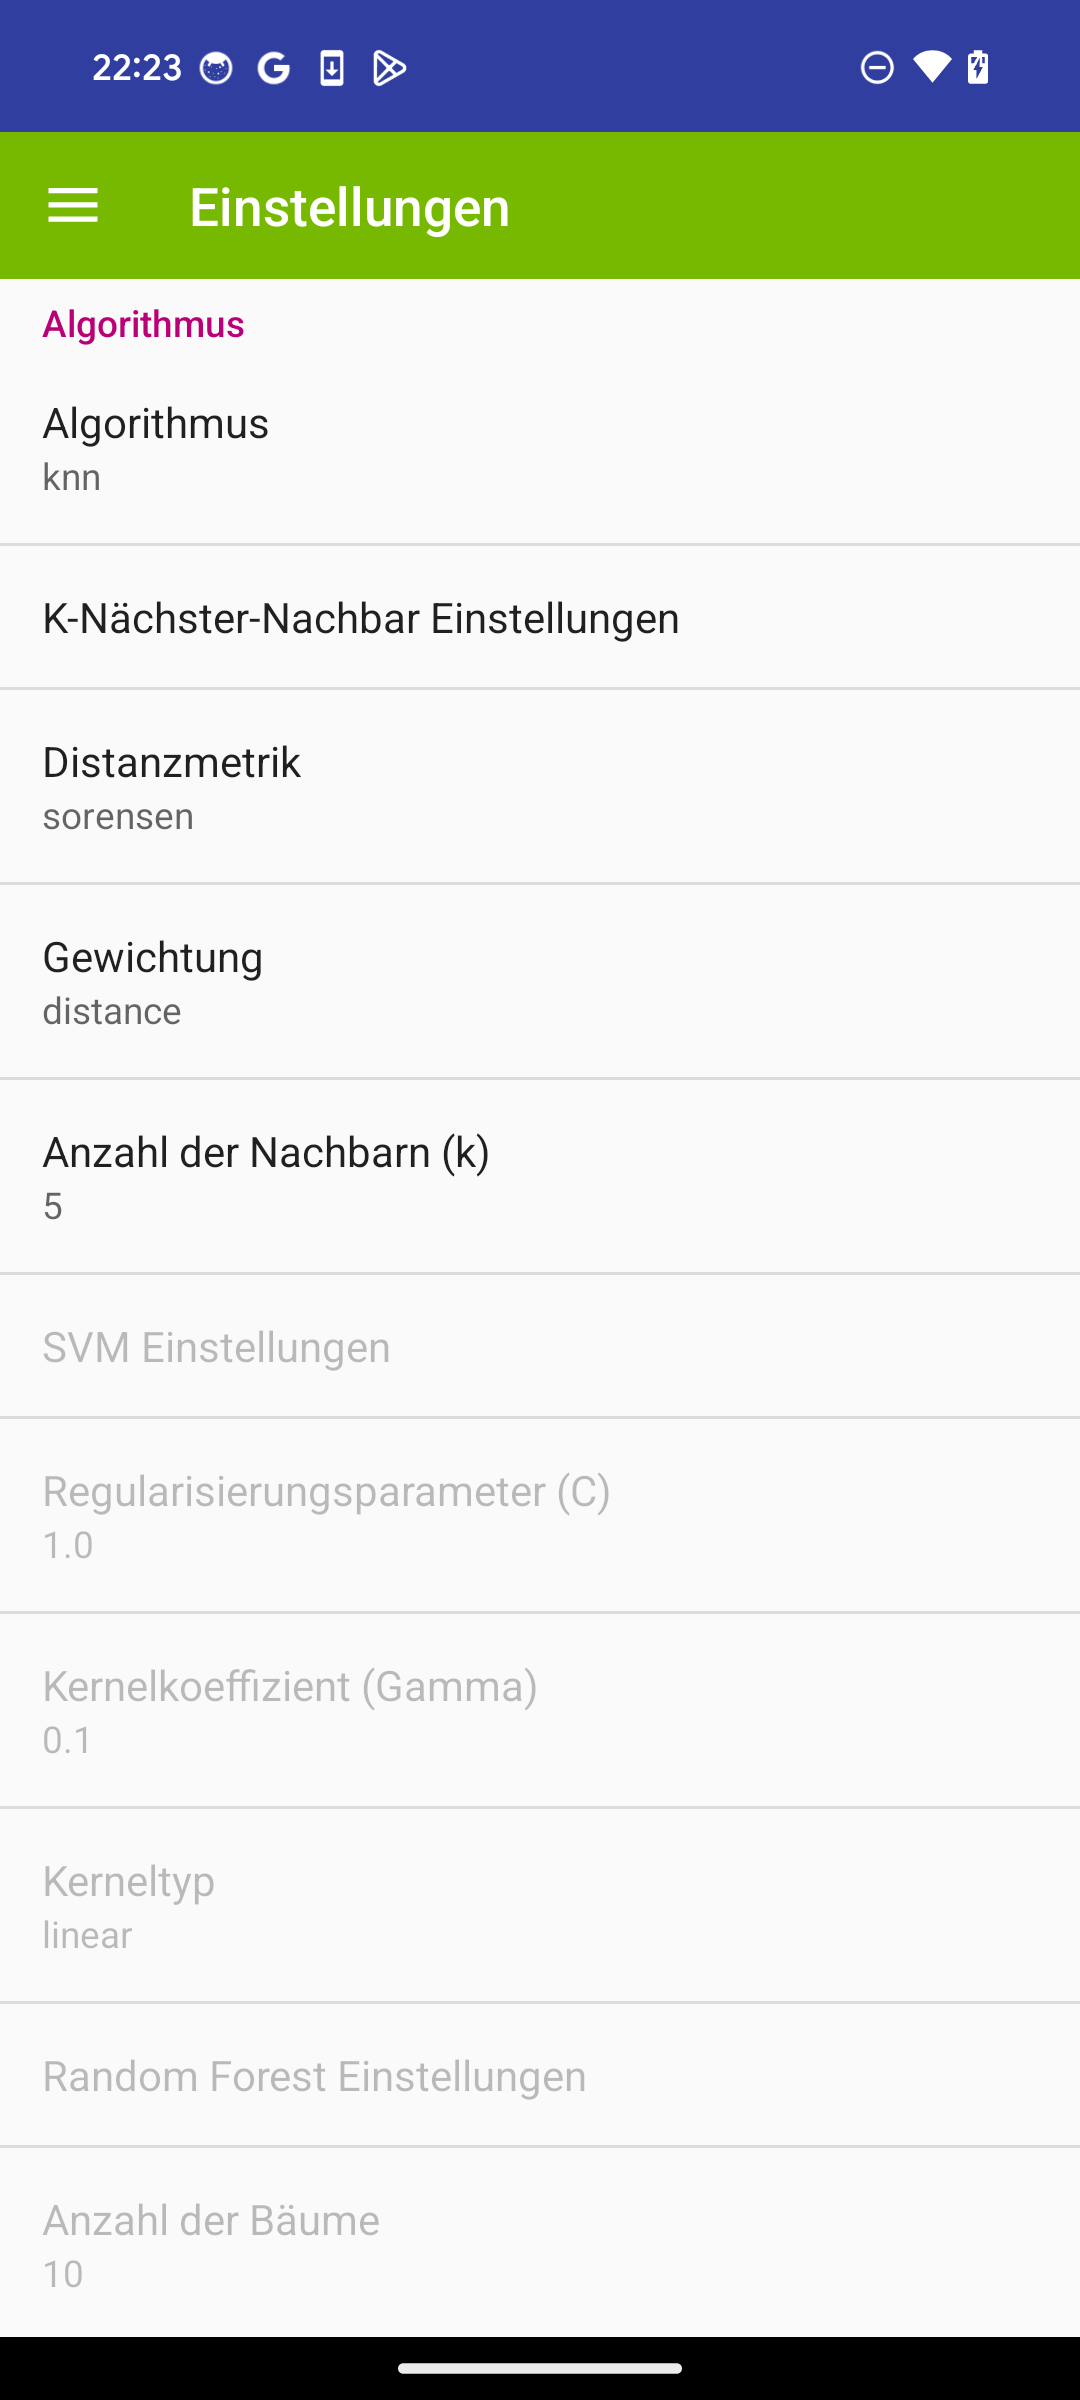
\includegraphics[width=\textwidth]{images/screenshots/settings_1.png}
        \caption{Einstellungen der Algorithmen und deren Parameter}
        \label{fig:app-localize-2}
    \end{subfigure}
    \hfill
    \begin{subfigure}[b]{0.3\textwidth}
        \centering
        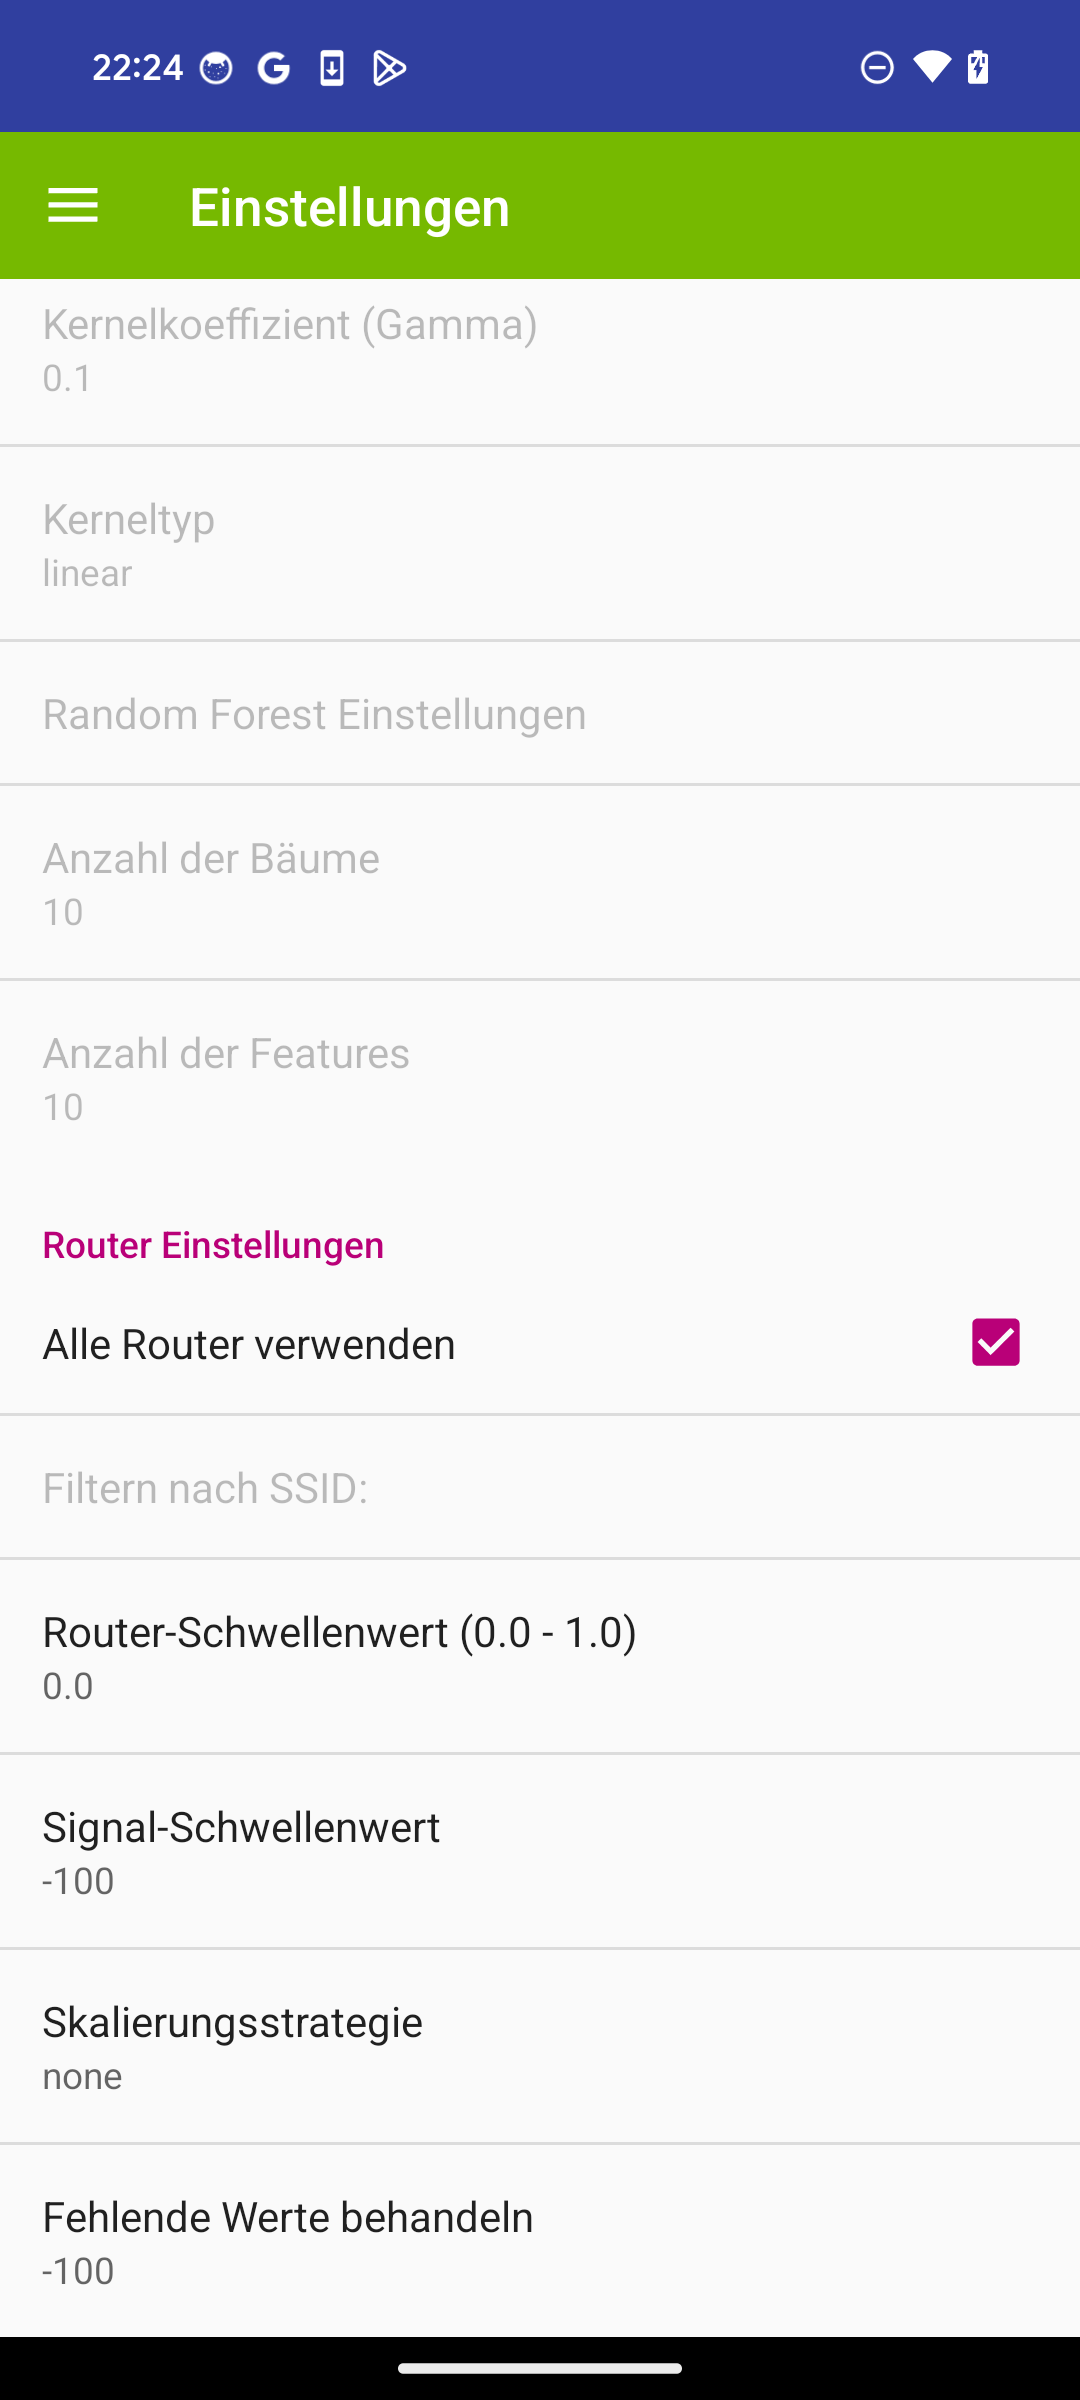
\includegraphics[width=\textwidth]{images/screenshots/settings_2.png}
        \caption{Übersicht der Access Points einer Messung}
        \label{fig:app-localize-3}
    \end{subfigure}
    \caption{Einstellungen der Datenaufbereitungsmethoden}
    \label{fig:app-localize-4}
\end{figure}

\section{Quellcode der Microcontroller}

Damit Microcontroller wie zum Beispiel der \textit{ESP32} seine Position bestimmen kann, muss dieser einen WiFi-Scan durchführen und die Daten an die API aus Kapitel \ref{api} senden. Dafür wurde ein \textit{MicroPython}-Script geschrieben, dass in dem Code Beispiel \ref{lst:esp32} dargestellt ist.

\begin{lstlisting}[caption={\textit{MicroPython}-Quellcode für die Durchführung eines WiFi-Scans und die Raumbestimmung über die API}, label={lst:esp32}]
import network
import urequests
import utime

# Initialize the Wi-Fi interface globally
wlan = network.WLAN(network.STA_IF)

# Function to connect to a Wi-Fi network
def connect_to_wifi(ssid, password):
    global wlan
    wlan.active(True)
    
    if not wlan.isconnected():
        print(f"Connecting to {ssid}...")
        wlan.connect(ssid, password)
        
        while not wlan.isconnected():
            print("Attempting to establish connection...")
            utime.sleep(1)
    
    print("Connected to Wi-Fi!")

# Function to scan available Wi-Fi networks and send the data to an API
def scan_and_send(api_route):
    global wlan
    
    # Scan for available networks
    networks = wlan.scan()
    
    # Prepare the data structure for the API
    routers = []
    for network in networks:
        bssid = ":".join("{:02x}".format(byte) for byte in network[1])
        signal_strength = network[3]
        ssid = network[0].decode('utf-8')
        
        if len(ssid) > 0:
            routers.append({
                "ssid": ssid,
                "bssid": bssid,
                "signal_strength": signal_strength
            })
    
    data = {
        "routers": routers
    }
    
    # Send the data via a POST request to the API
    try:
        response = urequests.post(api_route, json=data)
        if response.status_code == 200:
            response_json = response.json()
            print(f"Room Prediction: {response_json['room_name']}")
        else:
            print(f"Error in room prediction: {response.status_code} - {response.text}")
    except Exception as e:
        print(f"Error sending data: {e}")

# Main function
def main(ssid, password, api_route):
    connect_to_wifi(ssid, password)
    
    # Perform the Wi-Fi scan and send the data to the API
    scan_and_send(api_route)

if __name__ == '__main__':
    # Define SSID, password, and API route here
    ssid = 'Rechnernetze'
    password = ''
    api_route = 'http://141.45.212.246:8000/measurements/predict'
    
    main(ssid, password, api_route)
\end{lstlisting}    

\chapter{Datenerhebung und Analyse der Algorithmen} \label{datenerhebung_und_analyse}
% Der \gls{accesspoint} sendet die \gls{bssid} und die \gls{ssid}, damit Geräte, wie eine \gls{vm}, sich verbinden können. Algorithmen wie \gls{knn} und \gls{svm} können in einer \gls{api} implementiert werden, um die Datenverarbeitung zu optimieren.

% Für die Untersuchung der Algorithmen und deren Parameter wurde 

% Es werden Testdaten gesammelt, für diese werden dann Vorhersagen getroffen.... Also hier erklären was in dem Kapitel passiert.

% 1. Daten sammeln
% 2. Parameter bestimmt
% 3. 

\section{Aufnahme von WiFi-Fingerprints für die Analyse der Algorithmen} \label{datenerhebung}

% \subsection{Beschreibung der gesammelten Daten}

% Es wird die API ais Kapitel \ref{section-fastapi} verwendet.

% \begin{itemize}
%     \item \textbf{Datenerhebungsmethoden:} Erklären Sie, wie die Daten gesammelt wurden (z.B. welche Geräte, Orte und Zeitpunkte).
%     \item \textbf{Datensätze und Umfang:} Beschreiben Sie den Umfang und die Struktur der gesammelten Datensätze.
%     \item \textbf{Datenqualität und -validität:} Diskutieren Sie die Qualität und Validität der Daten.
% \end{itemize}

Für die Auswertung der Algorithmen und deren Parameter wurden 407 Messungen in 35 Räumen auf dem Campus Wilhelminenhof der Hochschule für Technik und Wirtschaft Berlin (HTW Berlin) in Gebäude C durchgeführt. Die Messungen fanden in dem Zeitraum vom 08. Mai 2024 bis zum 03. Juli 2024 statt und es wurden insgesamt 263 Router erfasst. Für die Aufnahme der WiFi-Fingerprints wurden ein Doogee Y8 und ein Google Pixel 8 Smartphone verwendet.

Die Messungen erfolgten dabei randomisiert, abhängig davon, welche Räume zu dem Zeitpunkt frei waren, und wurden hauptsächlich während der Pausenzeiten und am Abend durchgeführt, da zu diesen Zeiten die meisten Räume zur Verfügung standen. Dabei wurde bewusst darauf verzichtet, den genauen Standort innerhalb der Räume zu planen, um realistische Einsatzbedingungen widerzuspiegeln.

Eine Übersicht der Messungen pro Raum ist in Abbildung \ref{fig:0_general_01} dargestellt.

\begin{figure}[H]
    \centering
    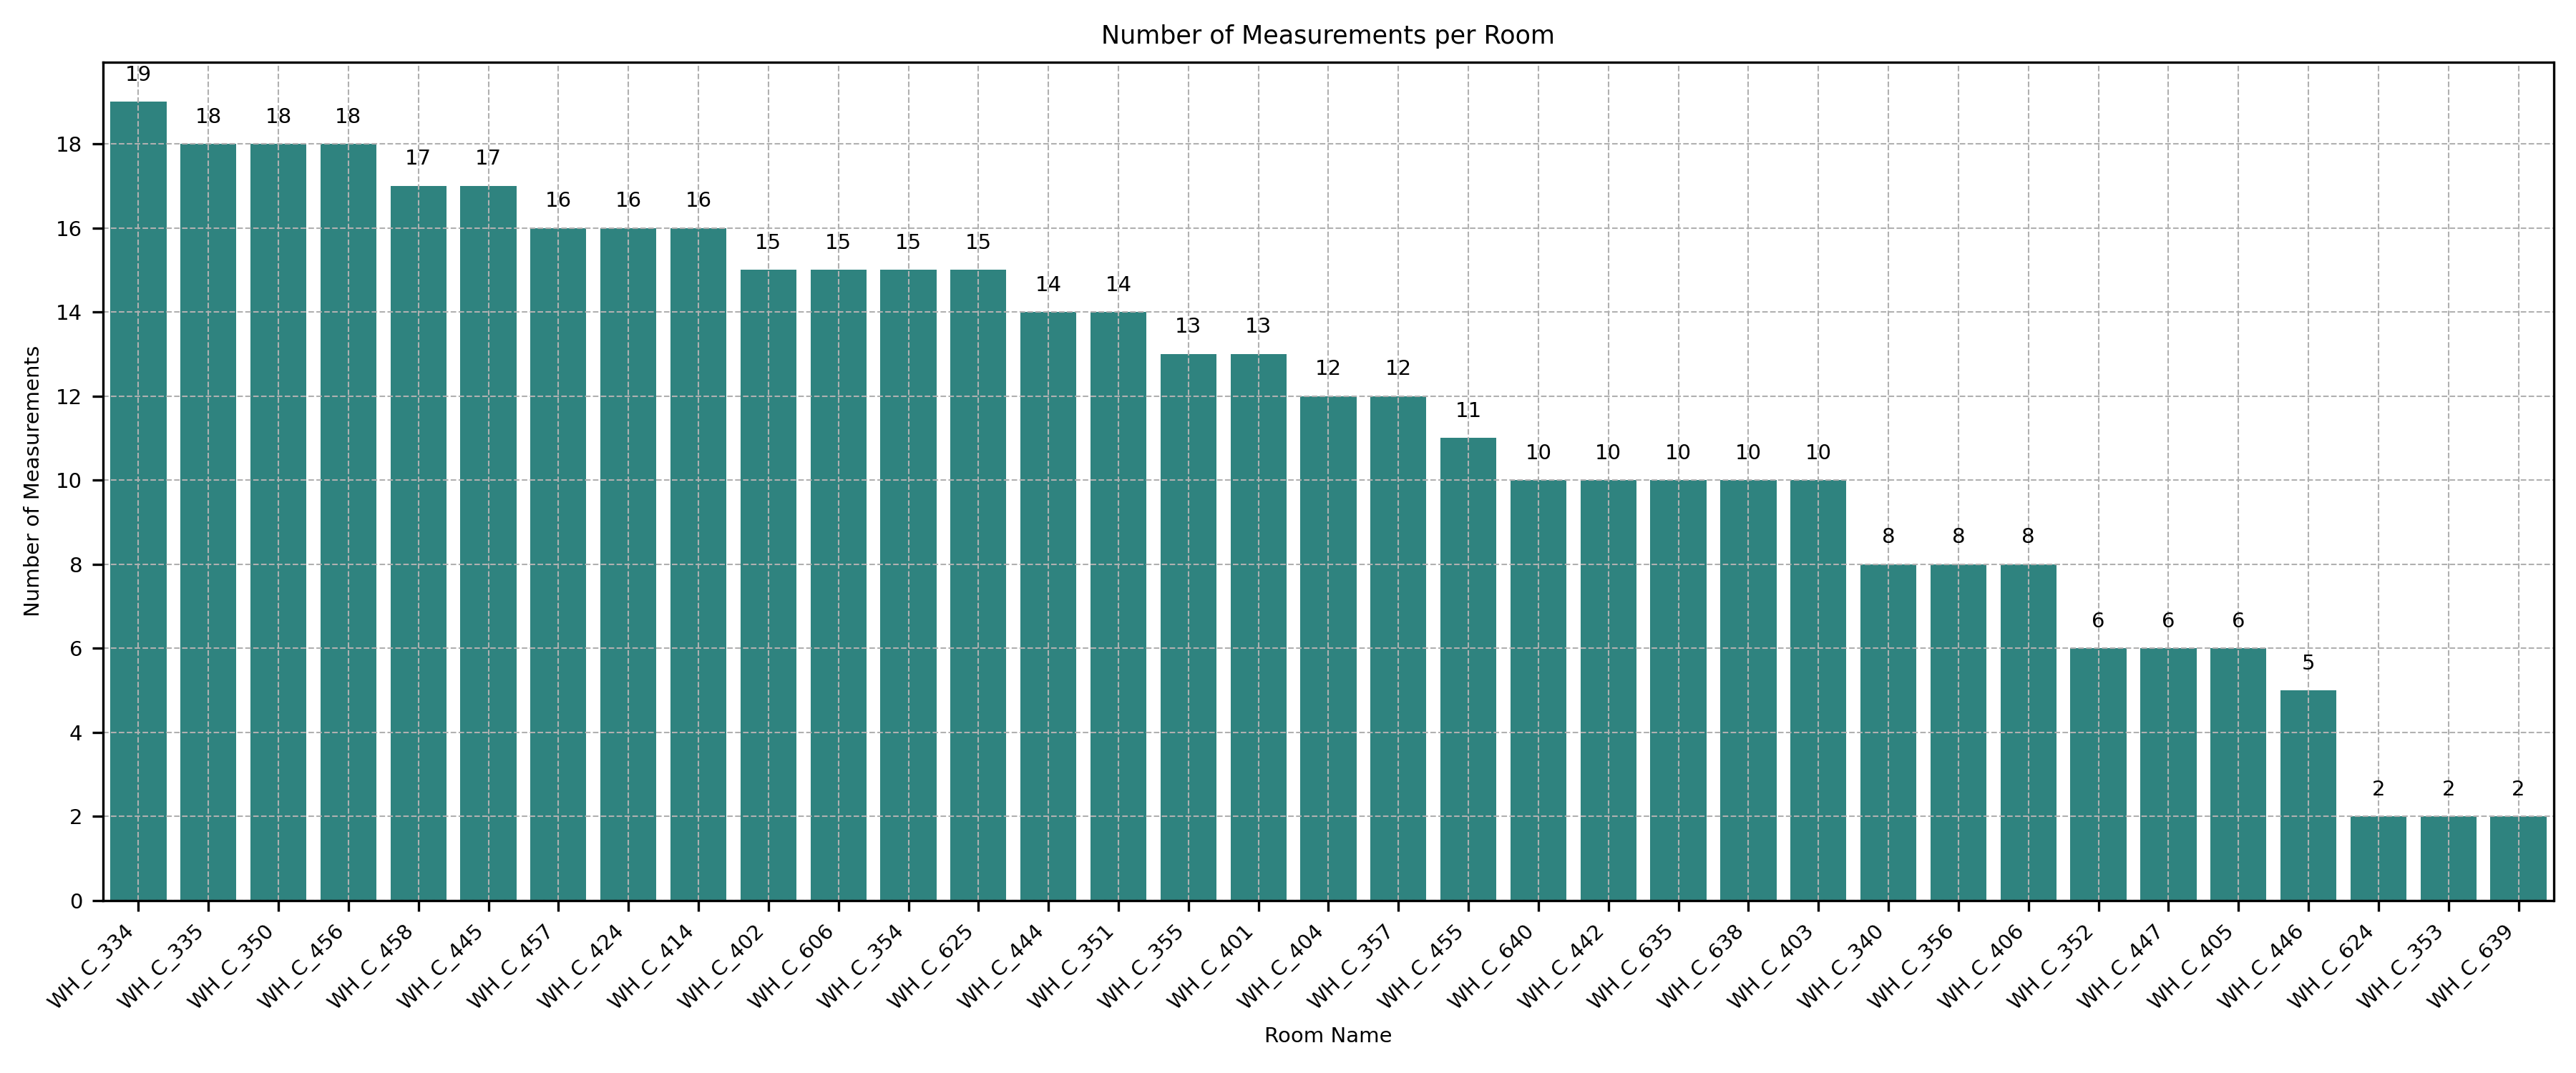
\includegraphics[width=0.8\textwidth]{images/00_general_01.png}
    \caption{Anzahl der Messungen pro Raum}
    \label{fig:0_general_01}
\end{figure}

\section{Beschreibung der Testanwendung} \label{testanwendung}

Für die Untersuchung der Modelle und deren Parameter wurde ein Anwendung in Python entwickelt, welche die verschiedenen Parameter der Algortihmen testet, indem alle möglichen Kombinationen der Parameter an die API gesendet werden und für jede Messung die Vorhersage gespeichert wird. Die Anwendung ist über eine \textit{YAML}-Datei (siehe Code-Beispiel \ref{lst:code_yaml}), in der die grundlegenden Einstellungen, wie die Endpunkte der API, die Anzahl der zu verarbeitenden Messungen und die zu betrachtenden Räume und Flure, definiert werden, konfigurierbar. 

Zudem können unter dem Parameter \textit{parameter\_sets} die verschiedenen Untersuchungsreihen definiert werden. Jeder Eintrag in \textit{parameter\_sets} entspricht einem Testlauf, dessen Ergebnisse unter dem angegebenen Namen in einer \textit{CSV}-Datei gespeichert werden. Innerhalb jedes Eintrags werden die zu testenden Parameter und deren Werte in einem Array angegeben.

In dem Code-Beispiel \ref{lst:code_yaml} sind zwei Testreihen definiert: \textit{01\_knn\_weights} und \textit{08\allowbreak\_router\allowbreak\_pre\-sence\allowbreak\_threshold}. In der ersten Testreihe werden für den \gls{knn}-Algorithmus mit der euklidischen und Sørensen Distanzmetrik und den Werten 5, 7 und 9 für den Parameter \textit{k\_value} die Gewichtungsfunktionen \textit{distance} und \textit{uniform} getestet. In der zweiten Testreihe wurden für den Parameter \textit{router\_presence\_threshold} die Werte 0, 0.25, 0.5 und 0.75 getestet und für die Algorithmen \gls{knn} mit der euklidischen Distanz und den Werten 5, 7 und 9 für den Parameter \textit{k\_value} und \gls{svm} mit dem RBF-Kernel und den Werten 5.0, 1.0 und 0.5 für den Parameter \textit{c\_value} untersucht.

Der Ablauf des Programms ist, dass zunächst die \textit{YAML}-Datei eingelesen, und über alle in den \textit{parameter\_sets} definierten Einträge iteriert wird. Für jeden Eintrag werden alle möglichen Kombinationen der angegebenen Parameter gebildet. Im Fall des zweiten Beispiels ergibt das 24 mögliche Kombinationen, da zwei Algorithmen mit jeweils drei unterschiedlichen Parametern und vier verschiedenen Werten für \textit{router\_presence\_threshold} getestet werden.

Anschließend durchläuft das Programm alle definierten Messungen (in diesem Beispiel 10) und sendet für jede dieser Messungen jede mögliche Parameterkombination über eine \textit{HTTP POST}-Anfrage an die API. Dabei wird auch die ID der jeweiligen Messung über den Parameter \textit{ignore\_measurements} mitgesendet, wodurch sichergestellt wird, dass diese Messung bei der Vorhersage nicht beachtet wird. Dies verhindert, dass die API eine Messung in der Datenbank findet, die exakt dem übermittelten Werten entspricht. Die Resultate der API-Anfragen werden nach dem Durchlauf aller Messungen in einer CSV-Datei, die nach dem Namen des jeweiligen \textit{parameter\_set}-Eintrags benannt ist, gespeichert.

\begin{lstlisting}[caption=\textit{YAML}-Konfigurationsdatei der Testanwendung, label={lst:code_yaml}]
url_fetch: "http://141.45.212.246:8000/measurements/all"
url_predict: "http://141.45.212.246:8000/measurements/predict"

num_measurements: 10
rooms: ["WH_C_351", "WH_C_352", "WH_C_353", "WH_C_335"]
corridors: ["WH_C_35_corridor"]

parameter_sets:
  - name: "01_knn_weights"
    parameters:
      weights: ["distance", "uniform"]
      algorithm:
        knn_euclidean:
          k_value: [5, 7, 9]
        knn_sorensen:
          k_value: [5, 7, 9]
  - name: "08_router_presence_threshold"
    parameters:
      router_presence_threshold: [0, 0.25, 0.5, 0.75]
      algorithm:
        knn_euclidean:
          k_value: [5, 7, 9]
        svm_rbf:
          c_value: [ 5.0, 1.0, 0.5]
\end{lstlisting}

\section{Analyse der Algorithmen und Parameter} \label{untersuchungen}

In dem folgenden Kapitel werden die verschiedenen Algorithmen und deren Parameter miteinander verglichen. Dafür wurde mithilfe der in Kapitel \ref{testanwendung} vorgestellten Anwendung für jede Untersuchung ein Eintrag in der \textit{YAML}-Konfigurationsdatei erstellt und es wurde für alle untersuchten Parameter und jede der 407 Messungen eine Vorhersage getroffen. 

\subsection{Voruntersuchung der nicht im Deatil betrachteten Parameter}

Da in dieser Arbeit für jeden Algorithmus ein Parameter im Detail untersucht wird und für jeden Algorithmus mehrere Parameter existieren, werden im ersten Schritt die Parameter untersucht, die nicht im Detail betrachtet werden. Das sind bei dem \gls{knn}-Modell der \texttt{weights} Parameter, der die Gewichtungsfunktion angibt, bei dem \gls{svm}-Modell mit dem RBF-Kernel der \texttt{gamma} Parameter und bei dem Random Forest Modell sind es die Parameter \textit{max\_depth} und \textit{n\_estimators}.

In Abbildung \ref{fig:1_distance_uniform_weights_01} sind die Ergebnisse des gewichteten und des ungewichteten \gls{knn}-Algorithmus in Abhängigkeit der Anzahl an Messungen pro Raum dargestellt. Wie zu erkennen ist, steigt die Genauigkeit mit der Anzahl an Messungen pro Raum, wobei der Unterschied zwischen \texttt{weights = distance} und \texttt{weights = uniform} mit zunehmender Anzahl an Messungen abnimmt und mit \texttt{weights = distance} bessere Ergebnisse erzielt werden konnten, wenn nur wenige Messungen vorhanden sind. Aus diesem Grund wurde sich dafür entschieden für die weiteren Untersuchungen den \texttt{weights} Parameter auf \texttt{distance} zu setzen.

\begin{figure}[H]
    \centering
    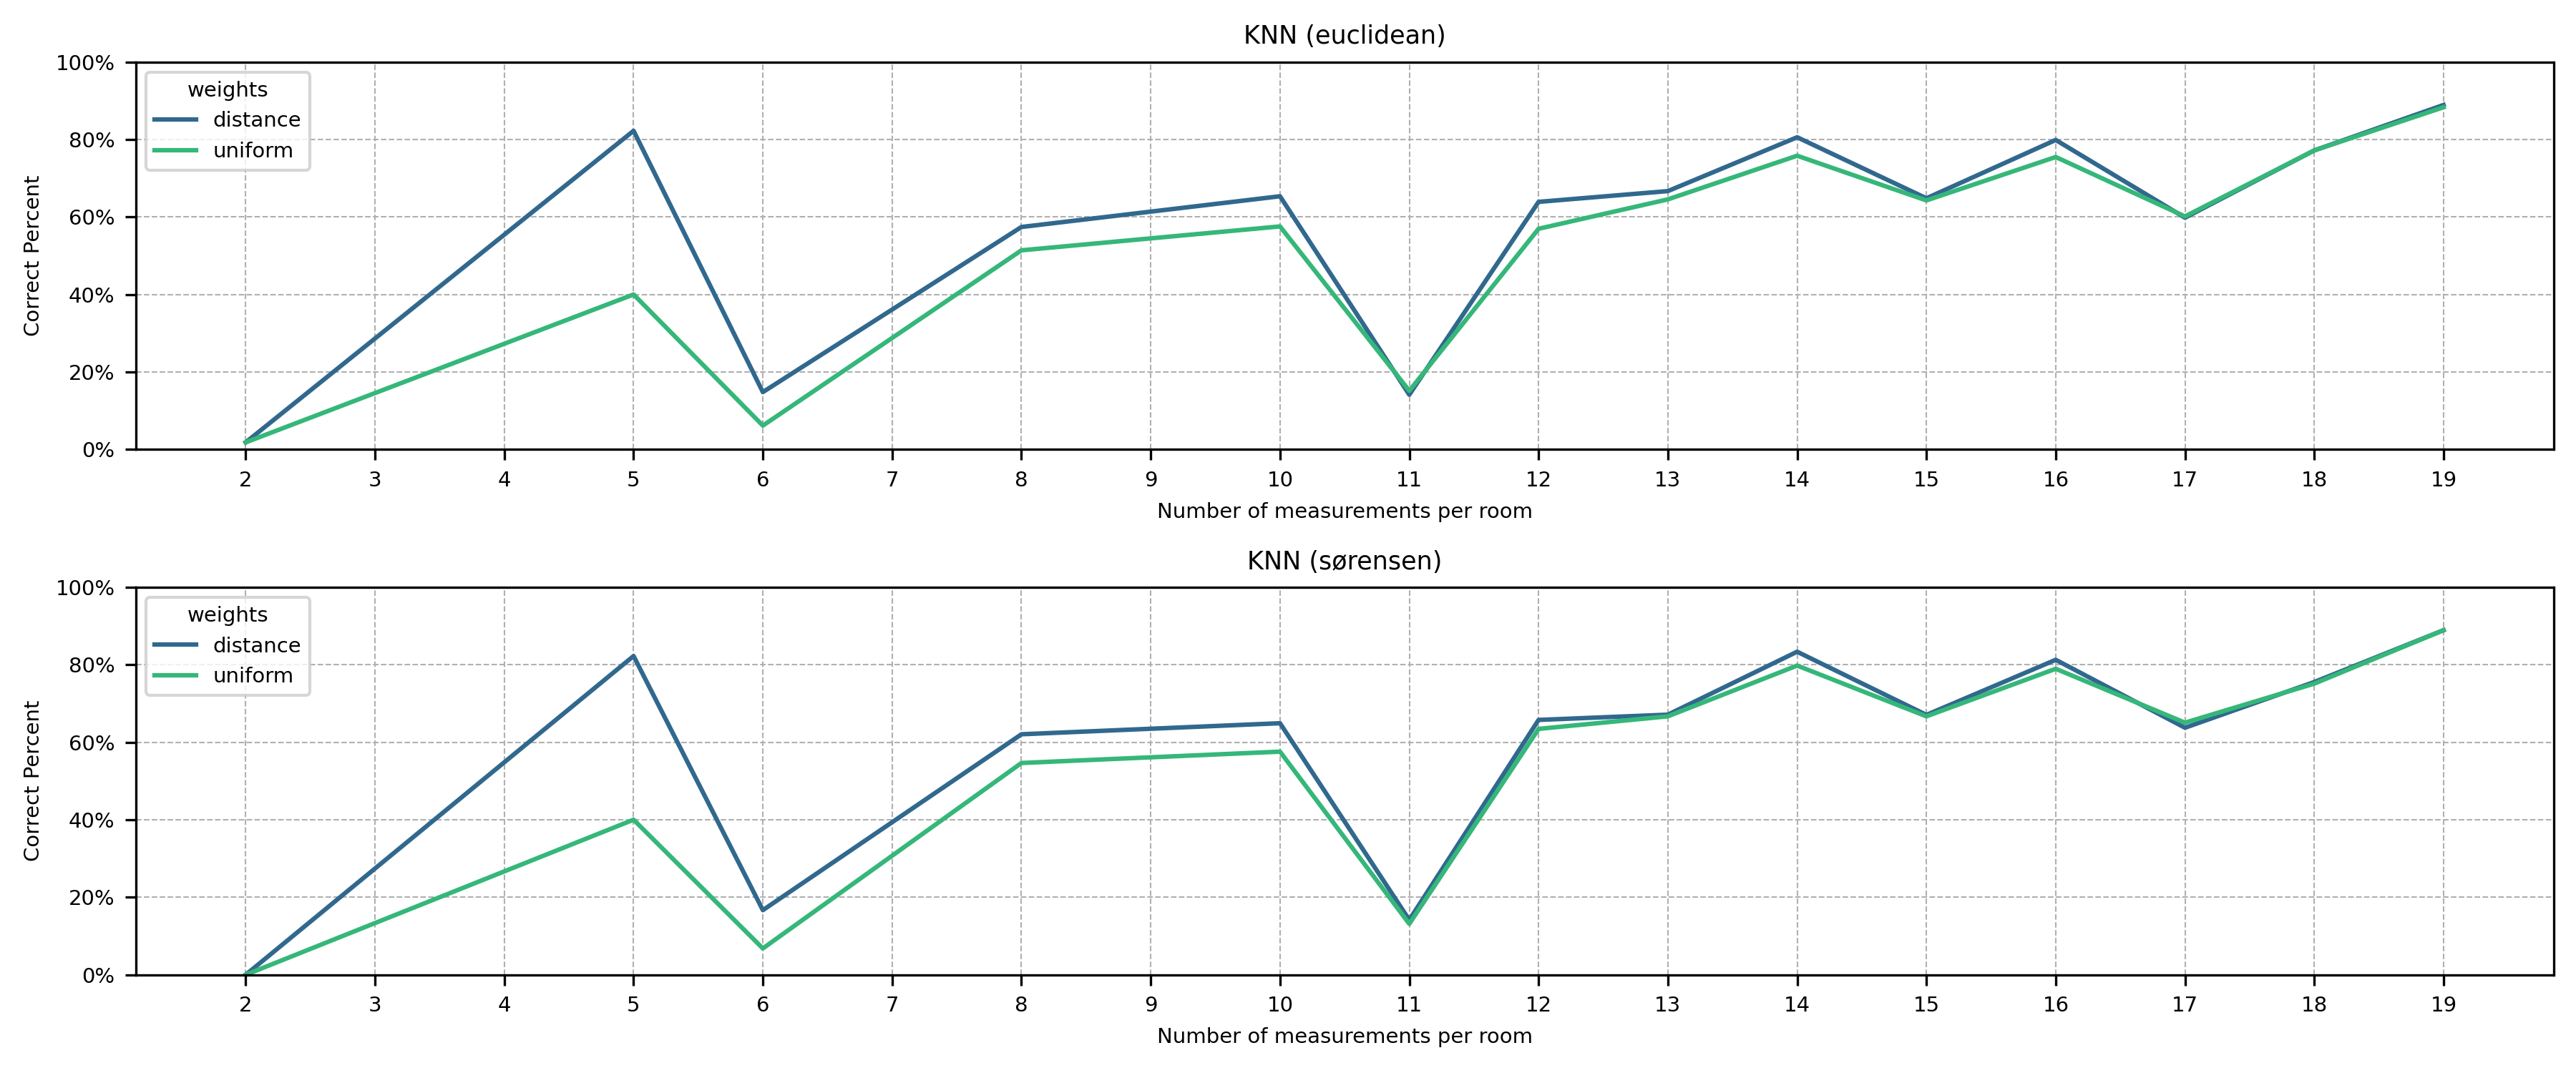
\includegraphics[width=0.8\textwidth]{images/01_knn_weights_01.png}
    \caption{Vergleich des gewichteten (\texttt{weights = distance}) und ungewichteten \gls{knn}-Algorithmus (\texttt{weights = uniform})}
    \label{fig:1_distance_uniform_weights_01}
\end{figure}


Bei dem \gls{svm} Algorithmus wurde der Parameter \texttt{gamma} untersucht, welcher nur für den RBF-Kernel gesetzt werden kann. Dabei wurde die Standardeinstellung von \texttt{scikit-learn}, welche \texttt{scale} ist, mit der Einstellung \texttt{auto} verglichen. Bei \texttt{scale} wird \texttt{gamma} auf

\begin{equation}
    \gamma = \frac{1}{n_{\text{features}} \cdot \text{Var}(X)}
\end{equation}

gesetzt und bei \texttt{auto} auf

\begin{equation}
    \gamma = \frac{1}{n_{\text{features}}}.
\end{equation}


\begin{figure}[H]
    \centering
    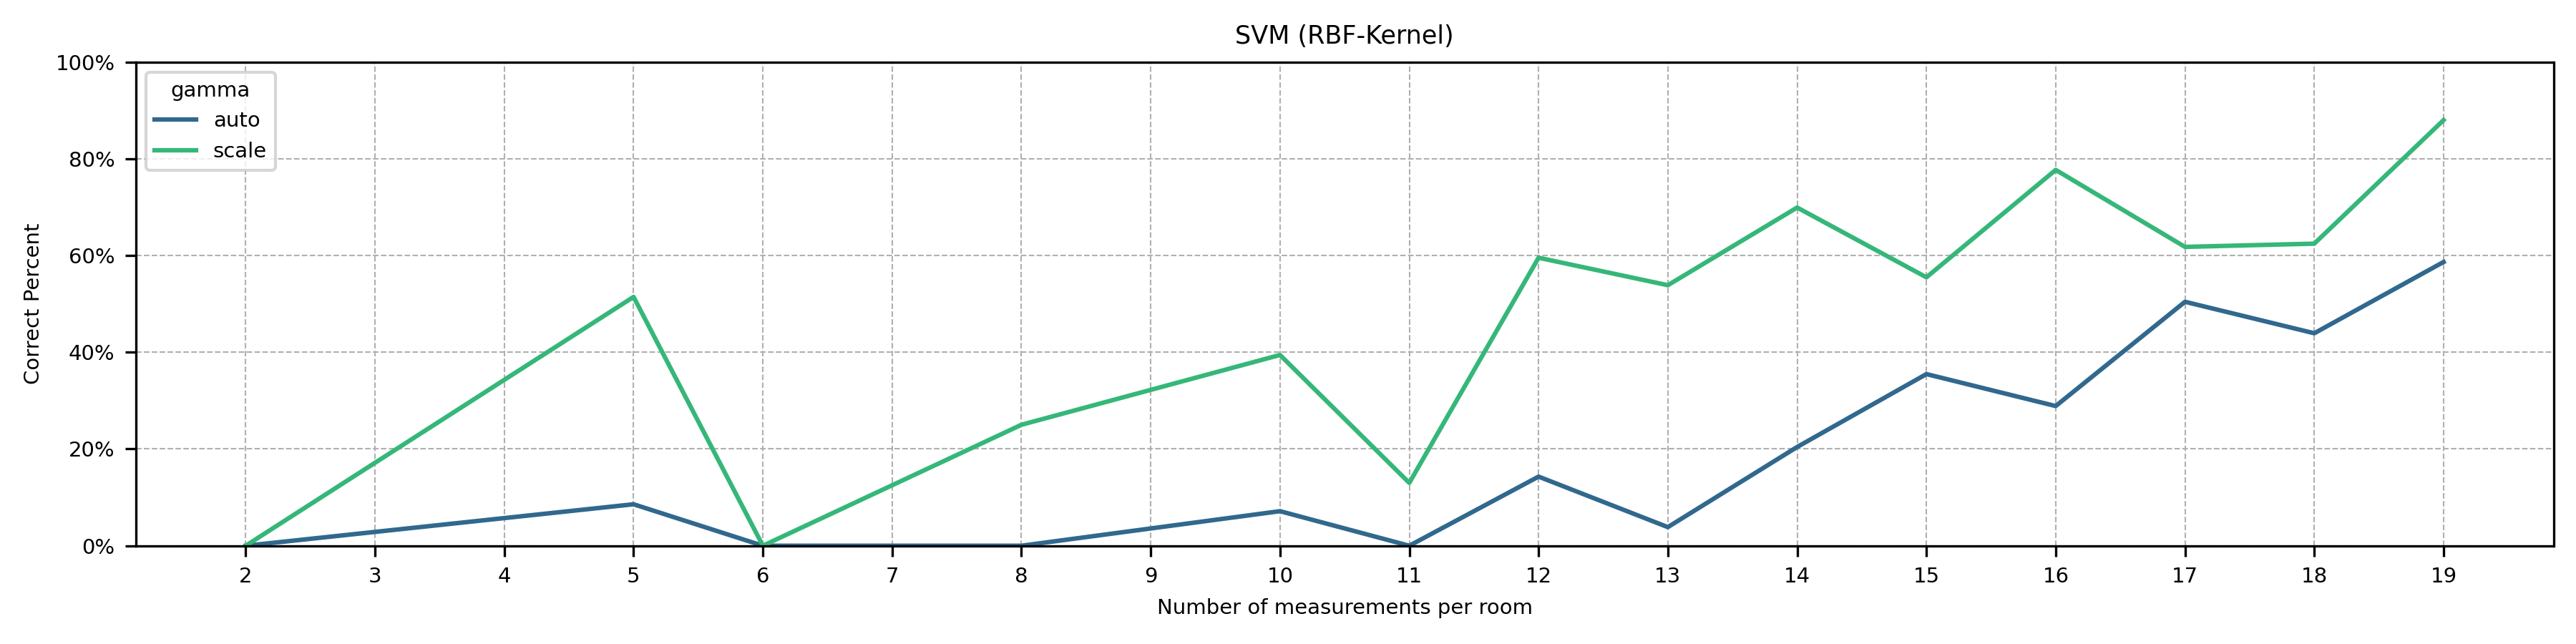
\includegraphics[width=0.8\textwidth]{images/02_svm_gamma_value_01.png}
    \caption{Vergleich der Parameter \texttt{auto} und \texttt{scale} des \texttt{gamma}-Parameters für den \gls{svm}-Algorithmus mit RBF-Kernel}
    \label{fig:1_best_parameters_svm_01}
\end{figure}

In Abbildung \ref{fig:1_best_parameters_svm_01} sind die Ergebnisse der beiden \texttt{gamma} Parameter in Abhängigkeit der Anzahl der Messungen pro Raum dargestellt. Wie zu erkennen ist, ist die Genauigkeit bei \texttt{scale} besser als bei \texttt{auto}. Aus diesem Grund wurde sich dafür entschieden für die weiteren Untersuchungen den \texttt{gamma} Parameter auf \texttt{scale} zu setzen.

% TODO: In welchem Wertebereich liegen die Werte?

% TODO:
% \begin{itemize}
%     \item Es muss auch irgendwo stehen was der average und der weighted average ist und warum beides in den Plots gezeigt wird!
% \end{itemize}

Bei Random Forest werden die beiden Parameter \texttt{max\_depth} (maximale Tiefe der Entscheidungsbäume) und \texttt{n\_estimators} (Anzahl der Entscheidungsbäume) untersucht, da diese laut dem Paper \textit{WiFi Indoor Localization with CSI Fingerprinting-Based Random Forest} neben dem Parameter \texttt{max\_features} (maximale Anzahl der verwendeten Features) den zweit- und drittgrößten Einfluss auf die Genauigkeit haben.\myfootcite{Wang2018WiFiLocalization}{S. 18}

Bei der Untersuchung der maximalen Tiefe der Entscheidungsbäume wurden für den Parameter \texttt{max\_depth} die Werte 1, 3, 5, 7, 9, 11, 13, 15, 17, 19, 21 und \texttt{None} verglichen. Grundlage für diese Entscheidung ist das Paper \textit{WiFi Indoor Localization with CSI Fingerprinting-Based Random Forest}, welches zu dem Ergebnis kam, dass die Genauigkeit der Ergebnisse ab einer bestimmten Tiefe der Entscheidungsbäume stagniert. Der Parameter \texttt{None} wurde zudem verwendet, da dies die Standardimplementierung von \texttt{scikit-learn} ist.\myfootcite{Wang2018WiFiLocalization}{S. 19}\textsuperscript{,}\mycitefoot{scikitlearnRandomForestClassifier}

\begin{figure}[H]
    \centering
    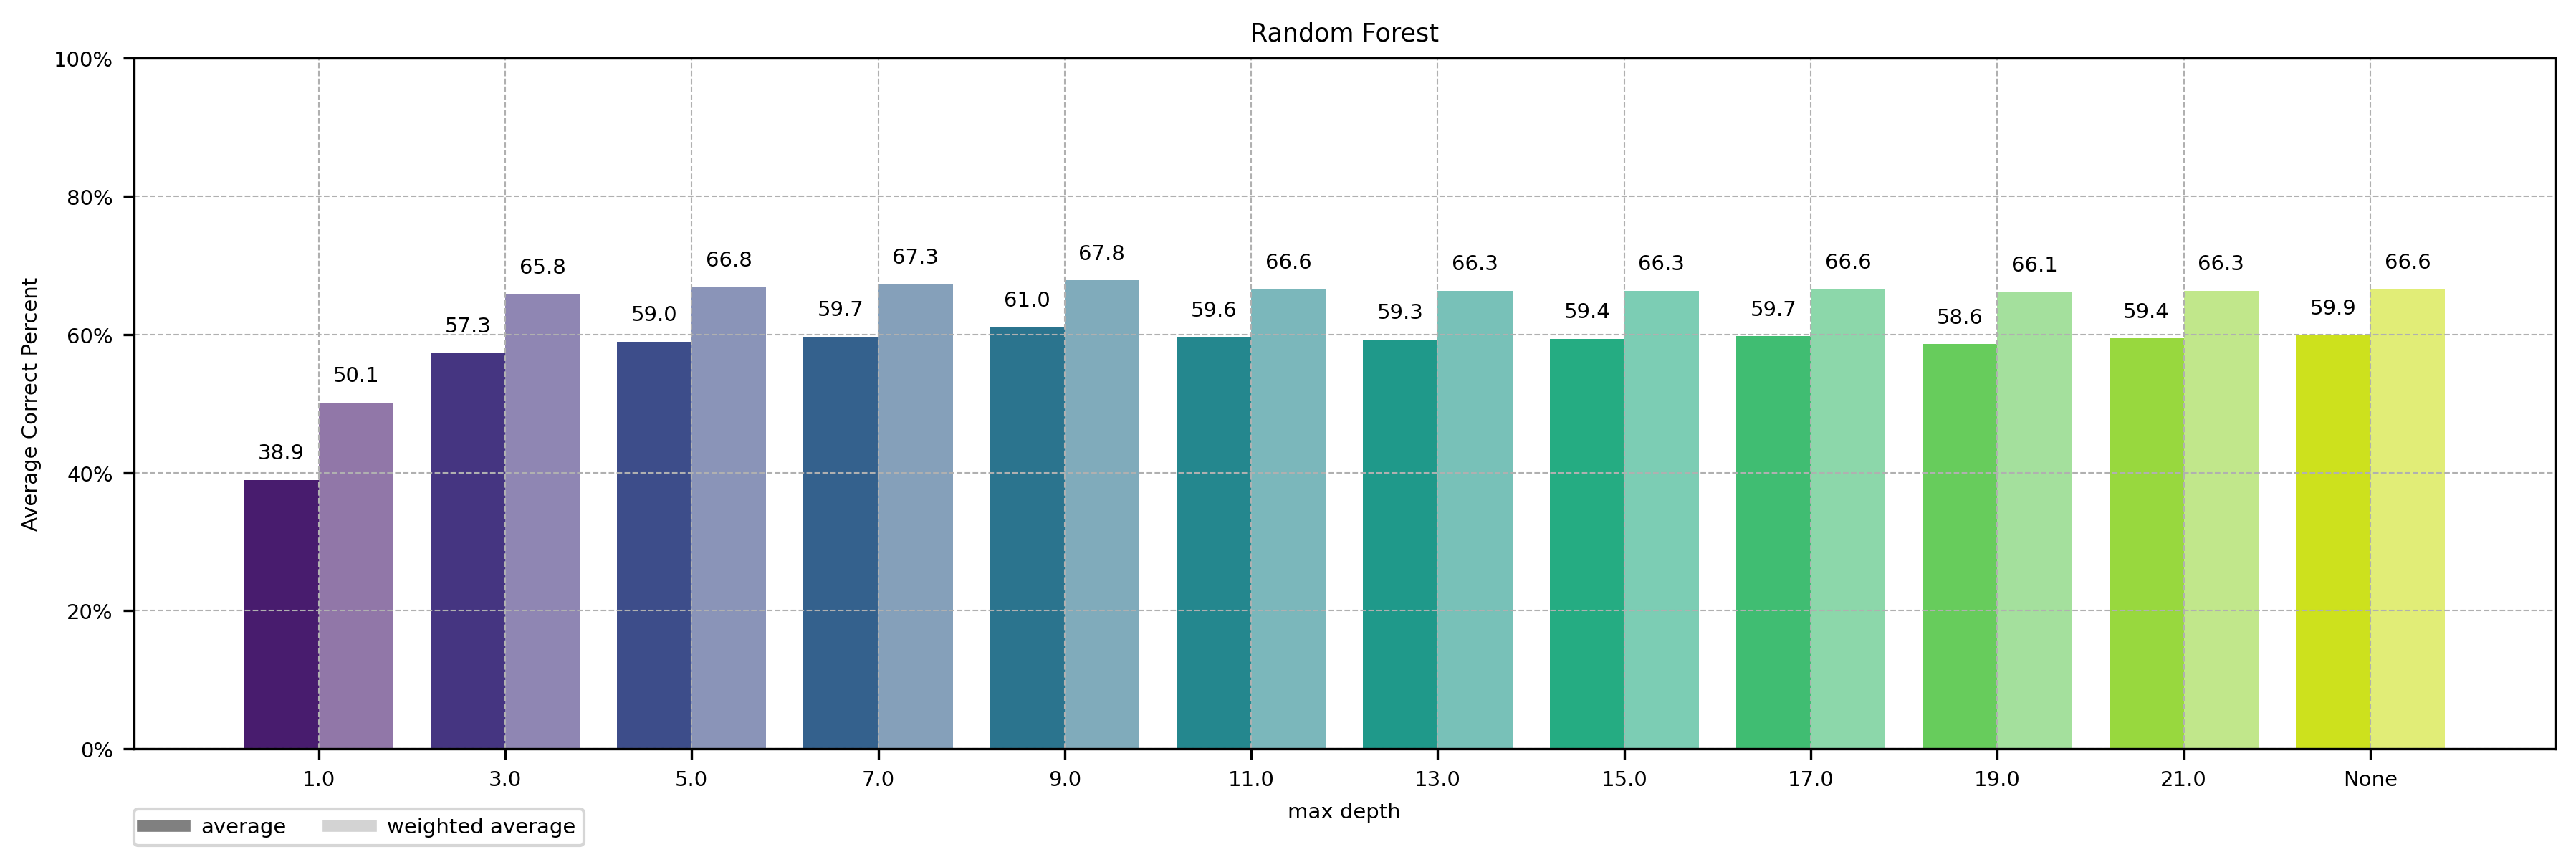
\includegraphics[width=0.8\textwidth]{images/03_random_forest_max_depth_03.png}
    \caption{Vergleich der verschiedenen Werte des \texttt{max\_depth} Parameters für den Random Forest Algorithmus}
    \label{fig:03_random_forest_max_depth_03}
\end{figure}

Wie in Abbildung \ref{fig:03_random_forest_max_depth_03} zu erkennen ist, hat die Wahl des Parameters nur einen geringen Einfluss auf die Genauigkeit der Ergebnisse, mit Ausnahme der Fälle, bei denen \texttt{max\_depth} auf 1 gesetzt ist. Bei allen anderen Werten sind die Genauigkeitsunterschiede minimal. Bei den ungewichteten Ergebnissen beträgt die maximale Abweichung 3,7 \%, während sie bei den gewichteten Ergebnissen bei 2 \% liegt.

Da die Genauigkeit ab einem bestimmten Wert des \texttt{max\_depth} Parameters keine signifikanten Unterschiede mehr aufweist und die besten Ergebnisse bei einer Teife von 9 erzielt werden konnte, wurde sich dafür entschieden für die weiteren Untersuchungen diesen Parameter auf 9 zu setzen.

% Random Forest (n\_estimators):

Bei der Auswahl der Anzahl der Bäume (\texttt{n\_estimators}) wurden die Werte in dem Wertebereich von 10 bis 100 in 10er-Schritten und die Werte in dem Wertebereich zwischen 100 und 1000 in 100er-Schritten untersucht. Diese Auswahl basiert auf den Erkenntnissen des Papers \textit{WiFi Indoor Localization with CSI Fingerprinting-Based Random Forest}, welches zeigt, dass die Genauigkeit mit zunehmender Anzahl an Bäumen zwar steigt, die Rechenzeit jedoch ebenfalls linear mit der Anzahl der Bäume wächst. Das Paper stellt außerdem fest, dass ab einer bestimmten Anzahl an Bäumen keine signifikanten Verbesserungen der Genauigkeit mehr erzielt werden und dass die Unterschiede bei einer geringen Anzahl von Bäumen größer sind.\myfootcite{Wang2018WiFiLocalization}{S. 19}

\begin{figure}[H]
    \centering
    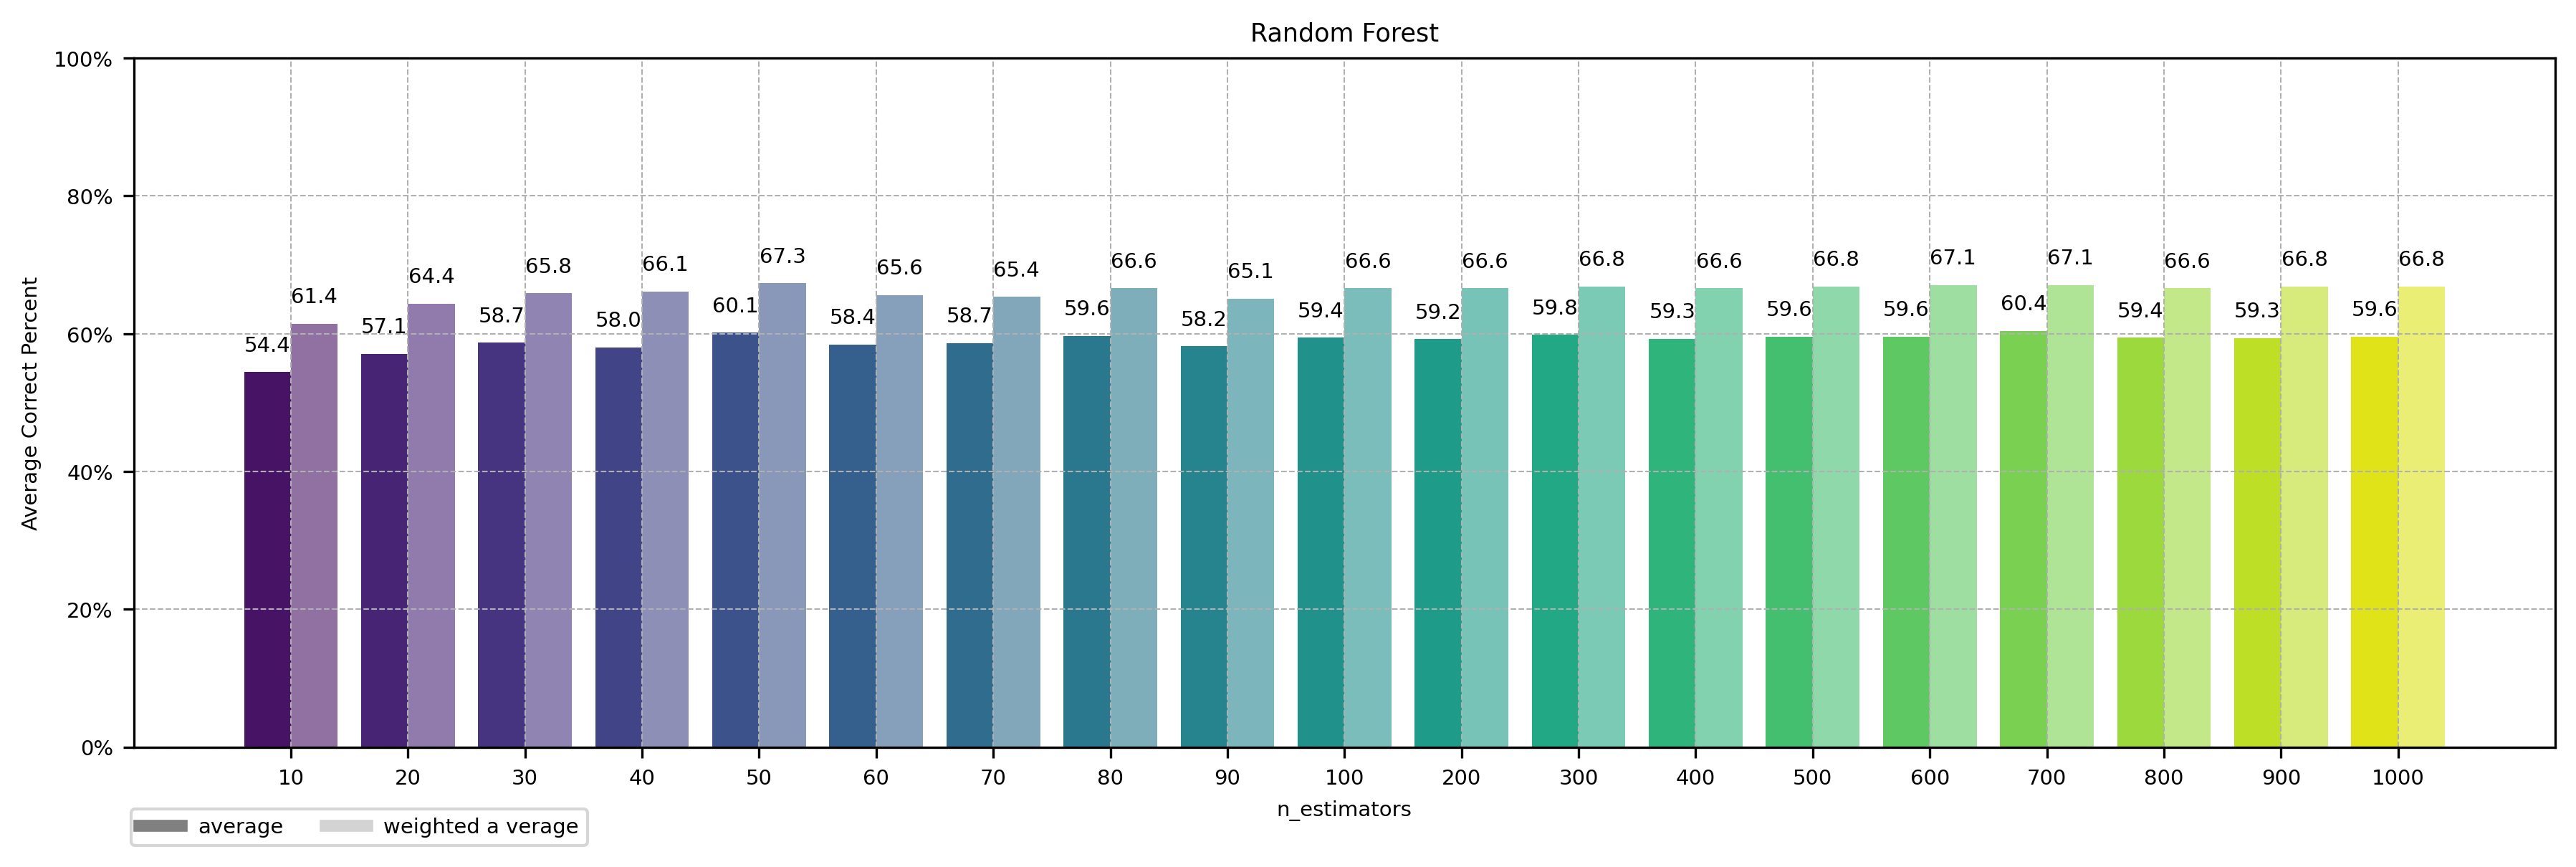
\includegraphics[width=0.8\textwidth]{images/04_random_forest_n_estimators_03.png}
    \caption{Vergleich der verschiedenen Werte des \texttt{n\_estimators} Parameters für den Random Forest Algorithmus}
    \label{fig:04_random_forest_n_estimators_03}
\end{figure}

\begin{figure}[H]
    \centering
    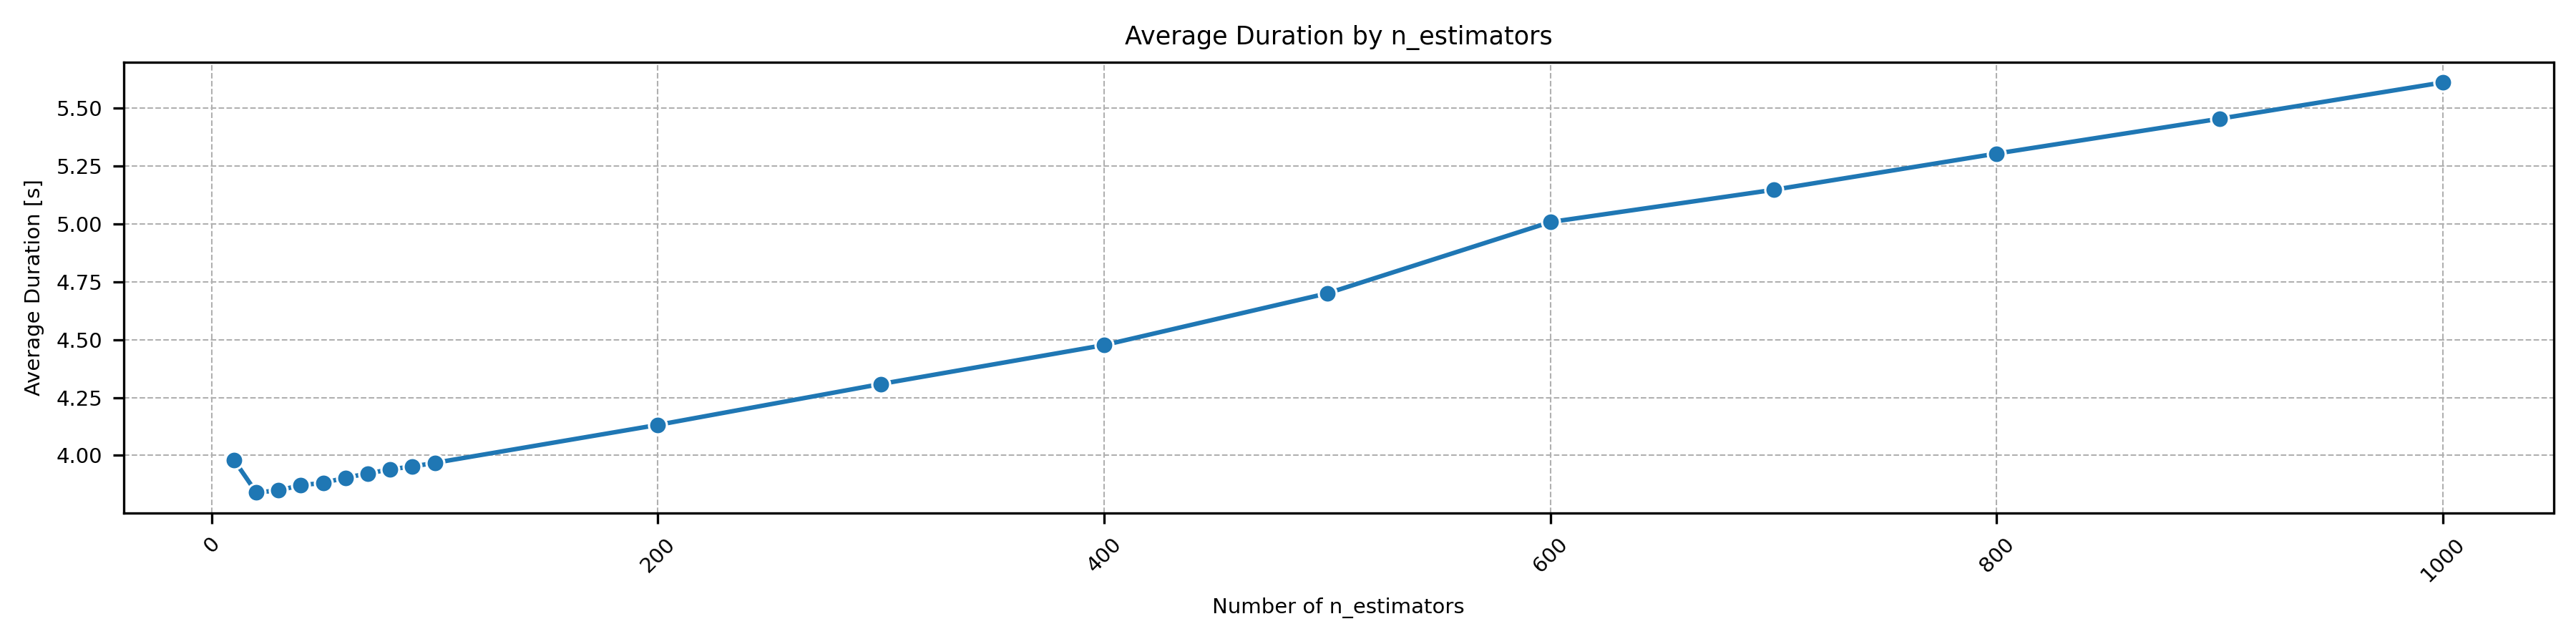
\includegraphics[width=0.8\textwidth]{images/04_random_forest_n_estimators_04.png}
    \caption{Vergleich der Dauer des Random Forest Algorithmus in Abhängigkeit der Anzahl der Bäume}
    \label{fig:04_random_forest_n_estimators_04}
\end{figure}

Wie in Abbildung \ref{fig:04_random_forest_n_estimators_03} zu erkennen ist, hat die Anzahl der Bäume, abgesehen von den kleineren Werten 10 und 20, keinen signifikanten Einfluss auf die Genauigkeit der Ergebnisse. Selbst bei den kleineren Werten ist der Unterschied der Genauigkeit nur minimal, wobei eine Steigerung der Anzahl der Bäume tendenziell zu einer höheren Genauigkeit führt. Die besten Ergebnisse wurden mit 50 Bäumen (60,1 \% ungewichteter Durchschnitt und 67,3 \% gewichteter Durchschnitt) und 700 Bäumen (60,4 \% ungewichteter Durchschnitt und 67,1 \% gewichteter Durchschnitt) erzielt.

In Übereinstimmung mit den Ergebnissen des zitierten Papers, zeigt Abbildung \ref{fig:04_random_forest_n_estimators_04}, dass die Rechenzeit linear mit der Anzahl der Bäume ansteigt. Aufgrund dieser Tatsache und der Tatsache dass die Unterschiede in der Genauigkeit zwischen 50 und 700 Bäumen gering sind, wurde sich dafür entschieden, für die weiteren Untersuchungen die Anzahl der Bäume auf 50 zu setzen.

\subsection{Untersuchung der im Deatil betrachteten Parameter}

Für die detailierten Untersuchungen der Parameter wurden für jeden Algorithmus die drei Parameter ermittelt, die in den meisten Fällen eine richtige Vorhersage getroffen haben. Dafür wurden für den \gls{knn} Algorithmus der Parameter k untersucht, für den Random Forest Algorithmus die Parameter \texttt{max\_features} und für den \gls{svm} Algorithmus der Parameter C. 


Bei dem \gls{knn} Algorithmus mit der Sørensen und euklidischen Distanz wurden jeweils die Parameterwerte 1, 3, 5, 7, 9, 11, 13, 15 getestet, da empfolen wird für k ungerade Werte zu verwenden. Für den \gls{svm} Algorithmus wurden für den linearen- und den RBF-Kernel die Parameterwerte  0.001, 0.005, 0.01, 0.05, 0.1, 0.5, 1, 5 für C verwendet, da diese in dem Paper \textit{Supervised Learning-Based Indoor Positioning System Using WiFi Fingerprints} empfolen wurden.\myfootcite{supervisedLearningIndoorPositioning}{S. 62} Für den Random Forest Algorithmus wurden die Parameterwerte \textit{sqrt}, \textit{log2}, \textit{None}, 0.1, 0.2, 0.3, 0.4, 0.5, 0.6, 0.7, 0.8, 0.9, 1, 2, 3, 4, 5, 6, 7, 8, 9, 10 verglichen, da für den Parameter \texttt{max\_features} in der \textit{scikit-learn} Implementierung des Random Forest Algorithmus die Anzahl der Features als absoluter Wert (Parameterwert 1 bis 10) oder als relativer Wert in Abhängigkeit der Gesamtzahl an Features angegeben werden kann und beides untersucht werden soll. Die Werte 0,1 bis 0,9 entsprechen dabei der Prozentzahl der betrachteten Features und \textit{sqrt} und \textit{log2} entsprechen der Quadratwurzel bzw. dem Logarithmus zur Basis 2 der Gesamtanzahl an Features.


% scikitlearnRandomForestClassifier

% In Abbildung \ref{fig:2_best_parameters_01} sind die besten Parameter für die Algorithmen in Abhängigkeit der Anzahl der Messungen dargestellt. Die Parameter wurden durch die Anwendung des Testprogramms auf die gesammelten Daten ermittelt. Die Parameter wurden so gewählt, dass die Genauigkeit der Algorithmen maximiert wurde. In Abbildung \ref{fig:2_best_parameters_02} ist die durchschnittliche Genauigkeit der Parameter dargestellt. Die Genauigkeit wurde durch die Anwendung des Testprogramms auf die gesammelten Daten ermittelt.

In Abbildung \ref{fig:05_best_parameters_all_01} sind die Ergebnisse der verschiedenen Parameter für den \gls{knn} und \gls{svm} Algorithmus in Abhängigkeit von der Anzahl der Messungen pro Raum dargestellt. Es ist ersichtlich, dass alle Algorithmen bei 5 Messungen pro Raum verhältnismäßig gute Ergebnisse erzielen konnten, während hingegen bei 11 Messungen pro Raum vergleichsweise schlechtere Ergebnisse auftraten. Dies könnte auf einzelne Ausreißer oder Messfehler zurückzuführen sein. Ebenso ist es möglich, dass die Räume mit 5 Messungen unter besonders günstigen Bedingungen erfasst wurden. Nimmt man diese Ausreißer heraus, zeigt sich bei allen Algorithmen die Tendenz, dass die Genauigkeit der korrekten Raumvorhersage mit einer zunehmenden Anzahl an Messungen pro Raum steigt.

In Abbildung \ref{fig:05_best_parameters_all_03} sind die durchschnittlichen Genauigkeiten der Parameter dargestellt. Dabei wurde einmal der Durchschnitt aller Ergebnisse berechnet (\textit{average}) und einmal der gewichtete Durchschnitt (\textit{weighted average}), bei dem für jede Anzahl an Messungen pro Raum der Durchschnitt gebildet wurde und anschließend der Gesamtdurchschnitt. Dies soll einer möglichen Verzerrung entgegenwirken, da so Räume mit mehr Messungen nicht stärker ins Gewicht fallen.

\begin{figure}[H]
    \centering
    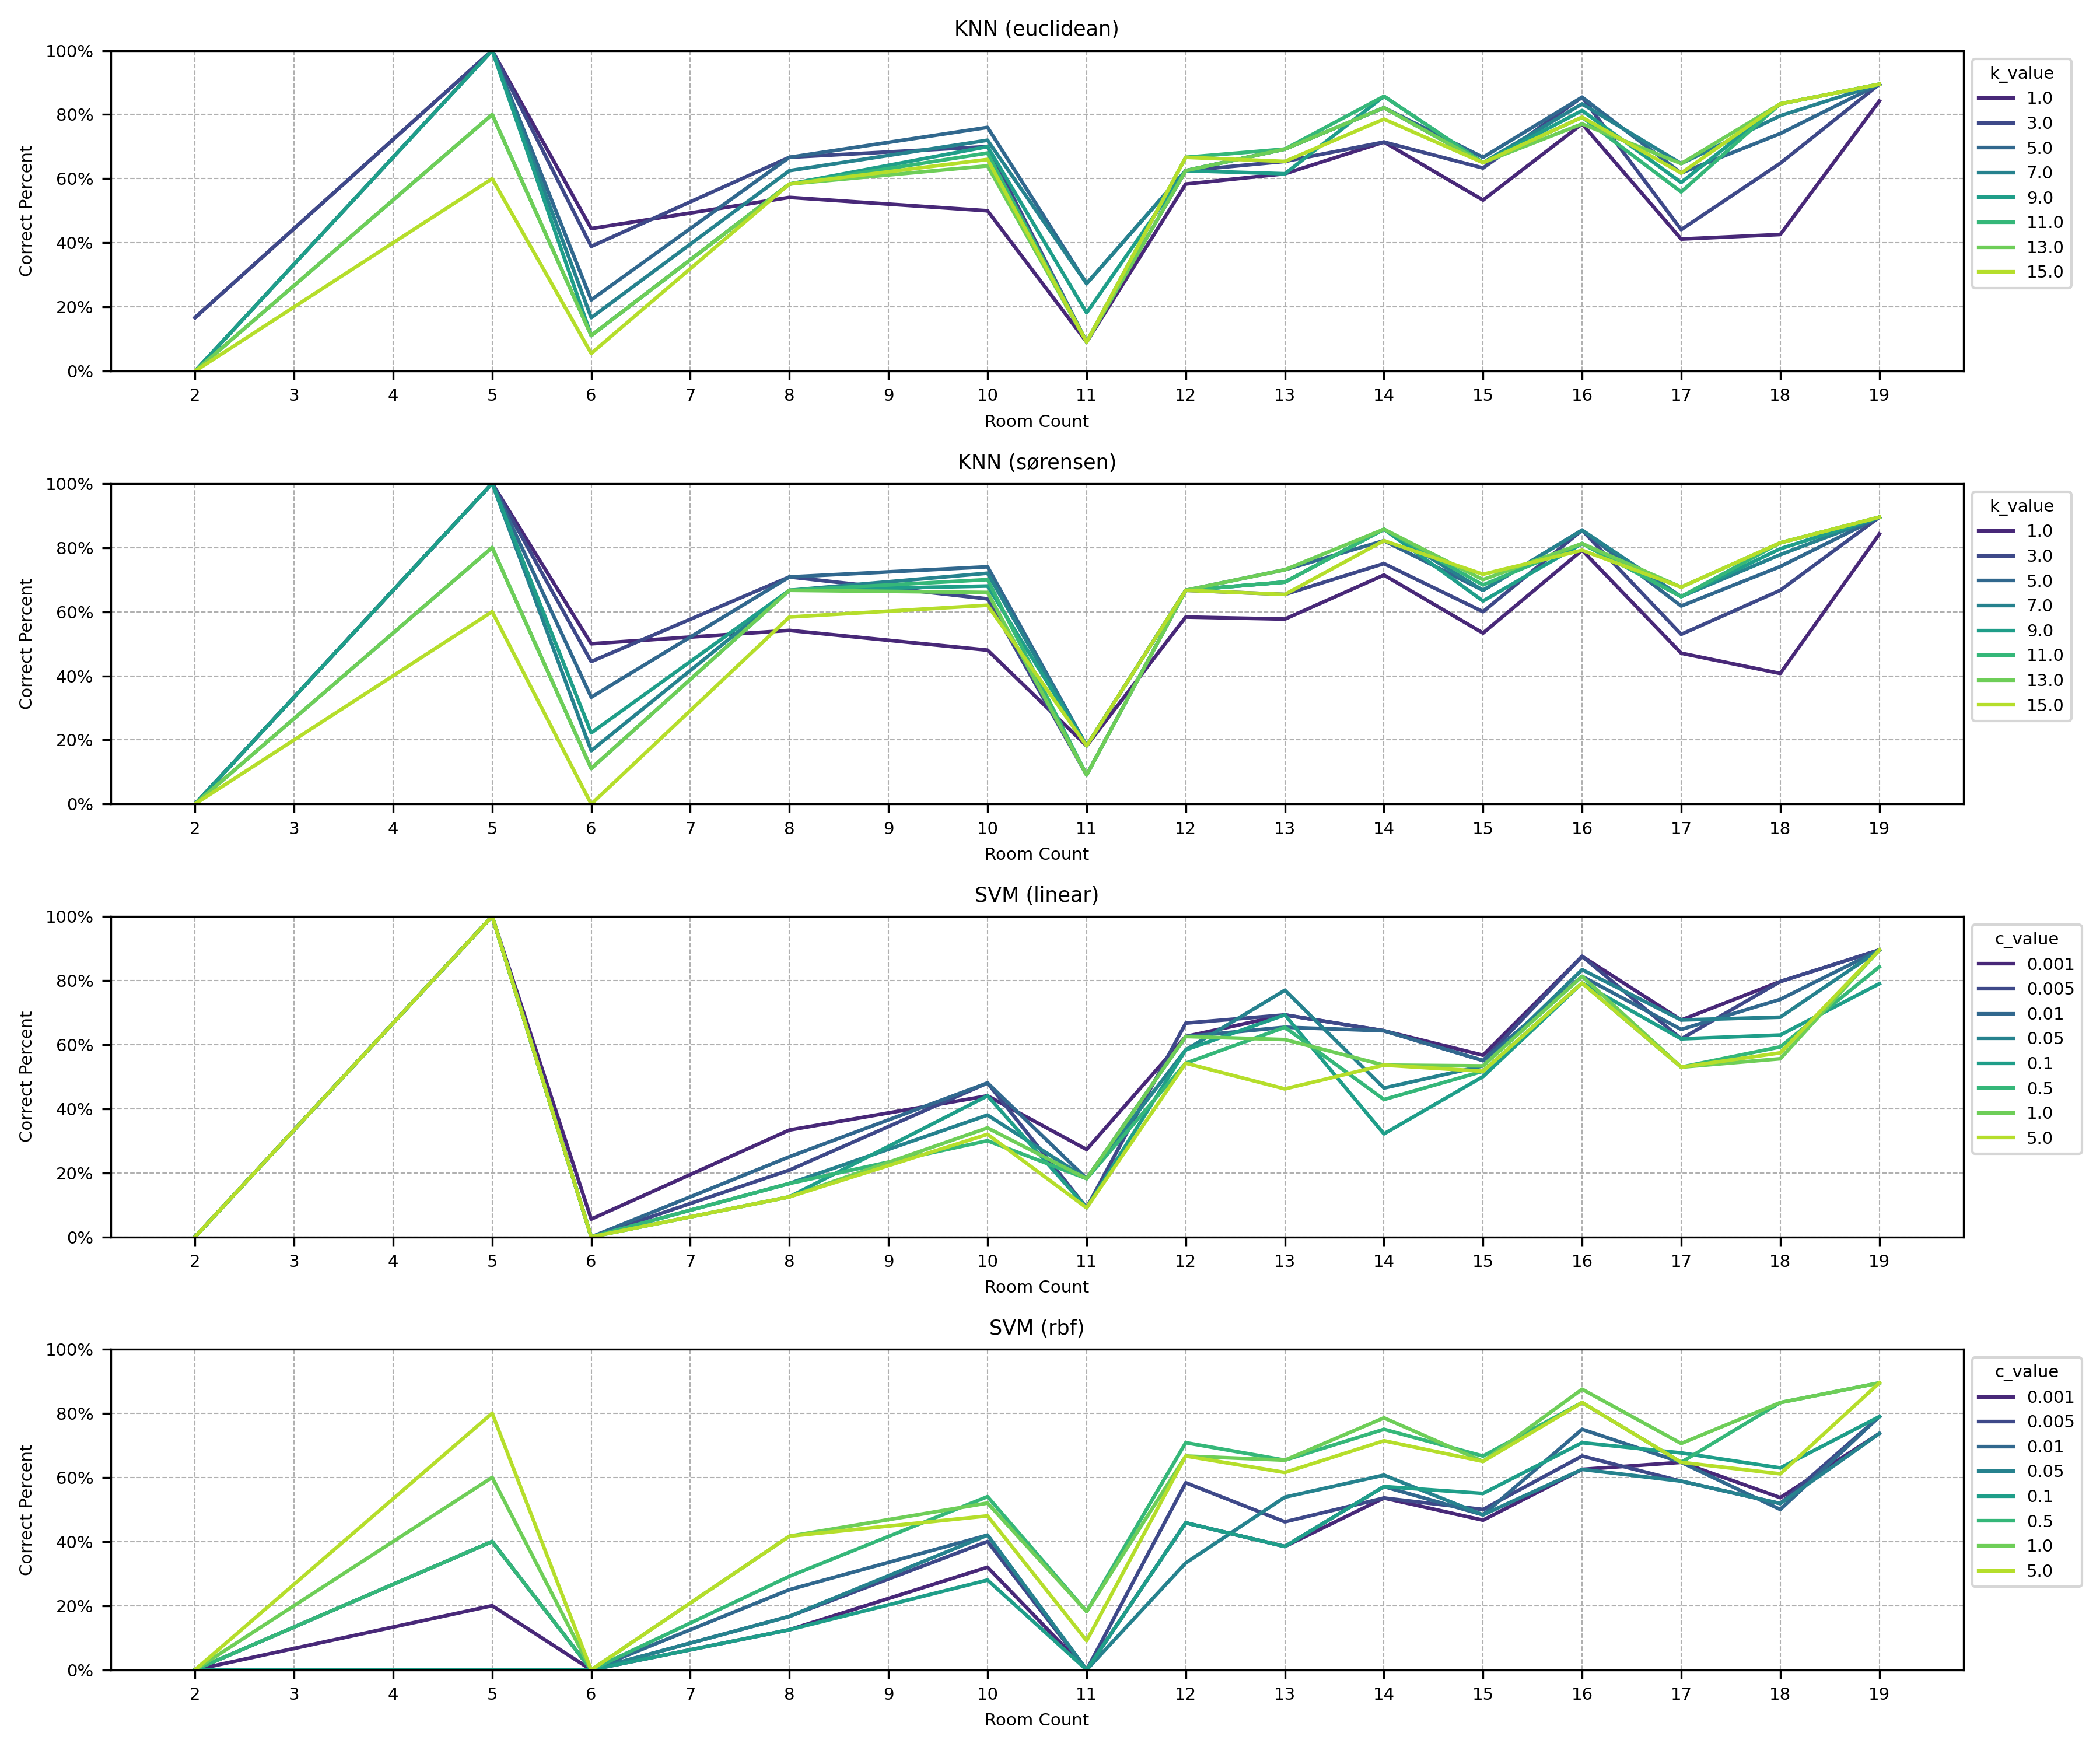
\includegraphics[width=0.8\textwidth]{images/05_best_parameters_all_01.png}
    \caption{Vergleich der Parameter in Abhängigkeit der Anzahl der Messungen}
    \label{fig:05_best_parameters_all_01}
\end{figure}

\begin{figure}[H]
    \centering
    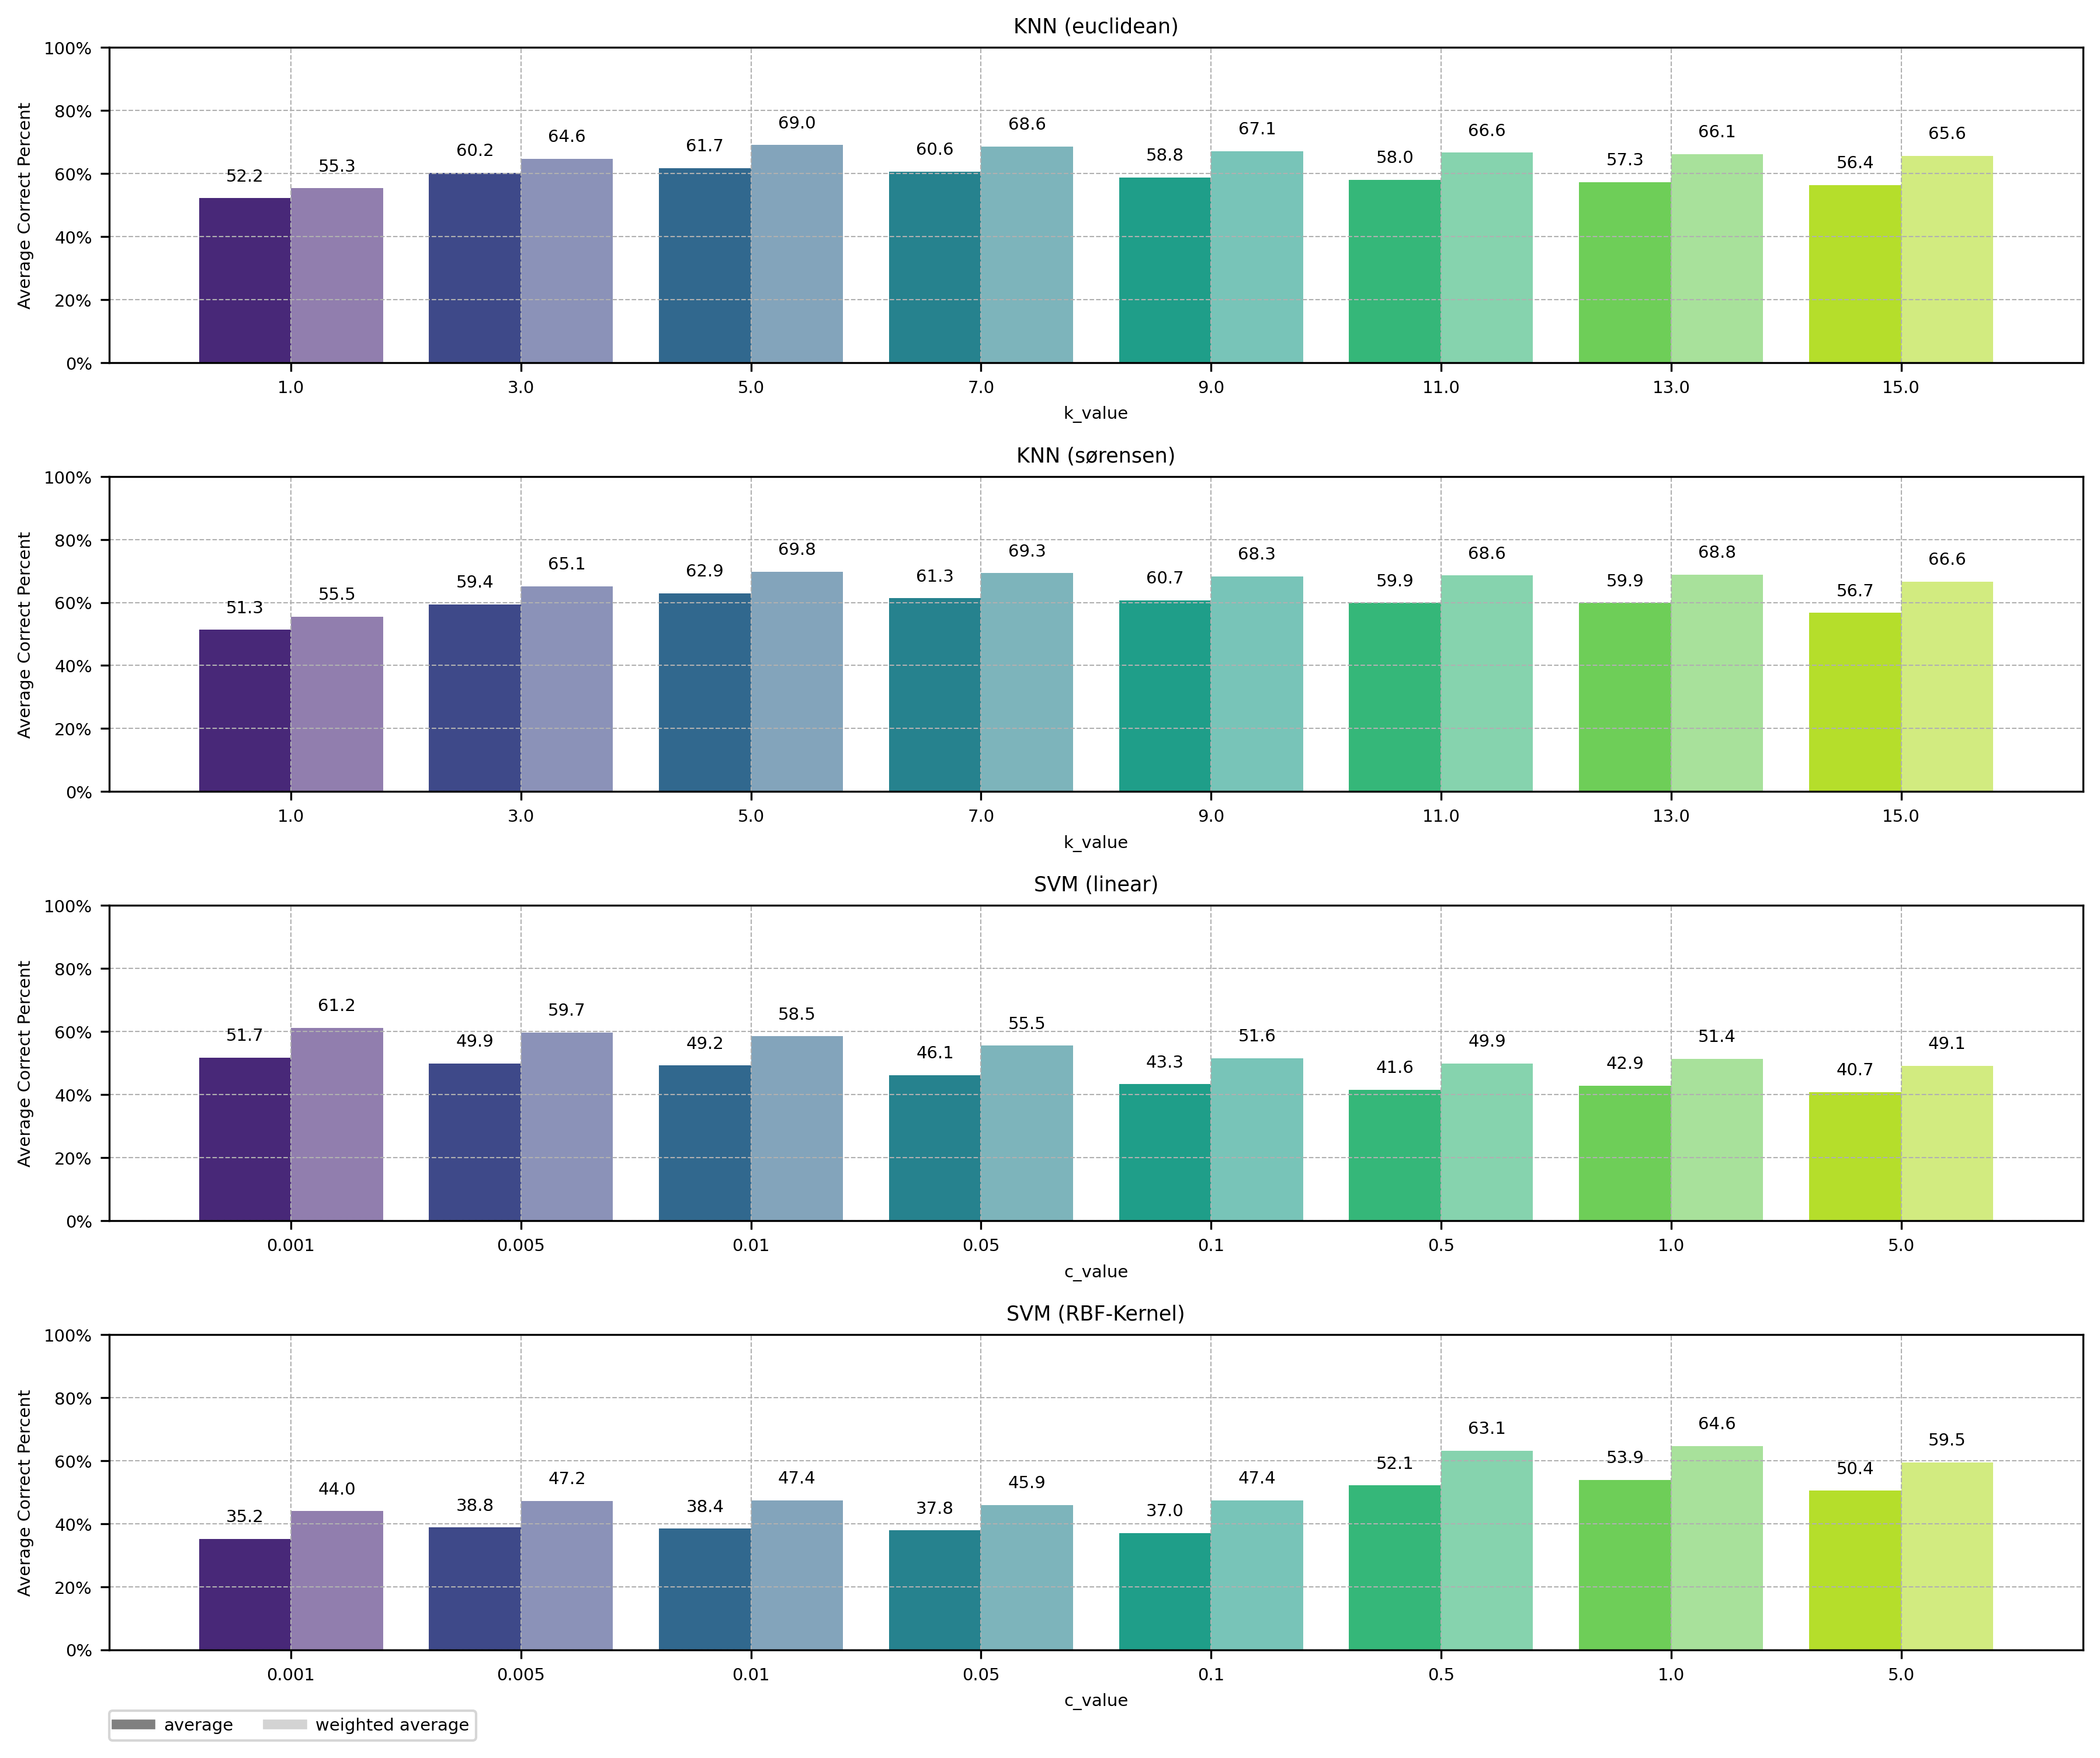
\includegraphics[width=0.8\textwidth]{images/05_best_parameters_all_03.png}
    \caption{Vergleich der durschnittlichen Genauigkeit der Parameter in Abhängigkeit der Anzahl der Messungen}
    \label{fig:05_best_parameters_all_03}
\end{figure}

% NICHT LÖSCHEN! WEIL QUELLE...
% Warum diese Parameter?
% \begin{itemize}
%     \item KNN: 1, 3, 5, 7, 9, 11, 13, 15 -> Weil ungerade (siehe Quelle bei KNN), im Wertebereich der Anzahl an Messungen pro Raum
%     \item RF: 50, 100, 150, 200, 250, 300, 350, 400 Wurde gewählt, weil 407 Messpunkte existieren
%     \item SVM: 0.001, 0.005, 0.01, 0.05, 0.1, 0.5, 1, 5 -> Quelle: Supervised Learning-Based Indoor Positioning System Using WiFi Fingerprints Seite 62
% \end{itemize}

% Ergebnisse:

% \begin{itemize}
%     \item KNN: 5, 7, 9
%     \item RF: 100, 200, 300
%     \item SVM (RBF): 0.5, 1, 5
%     \item SVM (Linear): 0.001, 0.005, 0.01
% \end{itemize}

\paragraph{\gls{knn}}

Wie in Abbildung \ref{fig:05_best_parameters_all_01} zu sehen ist, erzielen kleinere Werte für \( k \) sowohl bei der euklidischen als auch bei der Sørensen-Distanzmetrik bessere Ergebnisse in Räumen mit weniger Messungen, während größere Werte für \( k \) hingegen bei Räumen mit mehr Messungen von Vorteil sind. Im Durchschnitt konnten die besten Ergebnisse bei \( k = 5 \), \( k = 7 \) und \( k = 9 \) erzielt werden. Daher wurden diese Werte für die weiteren Analysen ausgewählt.

\paragraph{\gls{svm} (linear)}

Abbildung \ref{fig:05_best_parameters_all_03} zeigt, dass die Genauigkeit des \gls{svm}-Algorithmus mit linearem Kernel mit zunehmendem Wert für \( C \) abnimmt, wobei die besten Ergebnisse bei \( C = 0{,}001 \) erzielt wurden. Diese Ergebnisse gelten sowohl für den gewichteten (61,2 \%) als auch für den ungewichteten Durchschnitt (51,7 \%). Die zweit- und drittbesten Ergebnisse wurden für \( C = 0{,}005 \) und \( C = 0{,}01 \) erzielt. Daher wurden für die weitere Analyse die Werte \( C = 0{,}001 \), \( C = 0{,}005 \) und \( C = 0{,}01 \) ausgewählt.

\paragraph{\gls{svm} (RBF)}

Für den \gls{svm} Algorithmus mit dem RBF-Kernel wurden die besten Ergebnisse bei \( C = 1{,}0 \) erzielt (64,6 \% für den gewichteten und 53,9 \% für den ungewichteten Durchschnitt). Die zweit- und drittbesten Ergebnisse wurden bei \( C = 0{,}5 \) und \( C = 5{,}0 \) erreicht. Daher wurden für die weitere Analyse die Werte \( C = 0{,}5 \), \( C = 1{,}0 \) und \( C = 5{,}0 \) ausgewählt.

\begin{figure}[H]
    \centering
    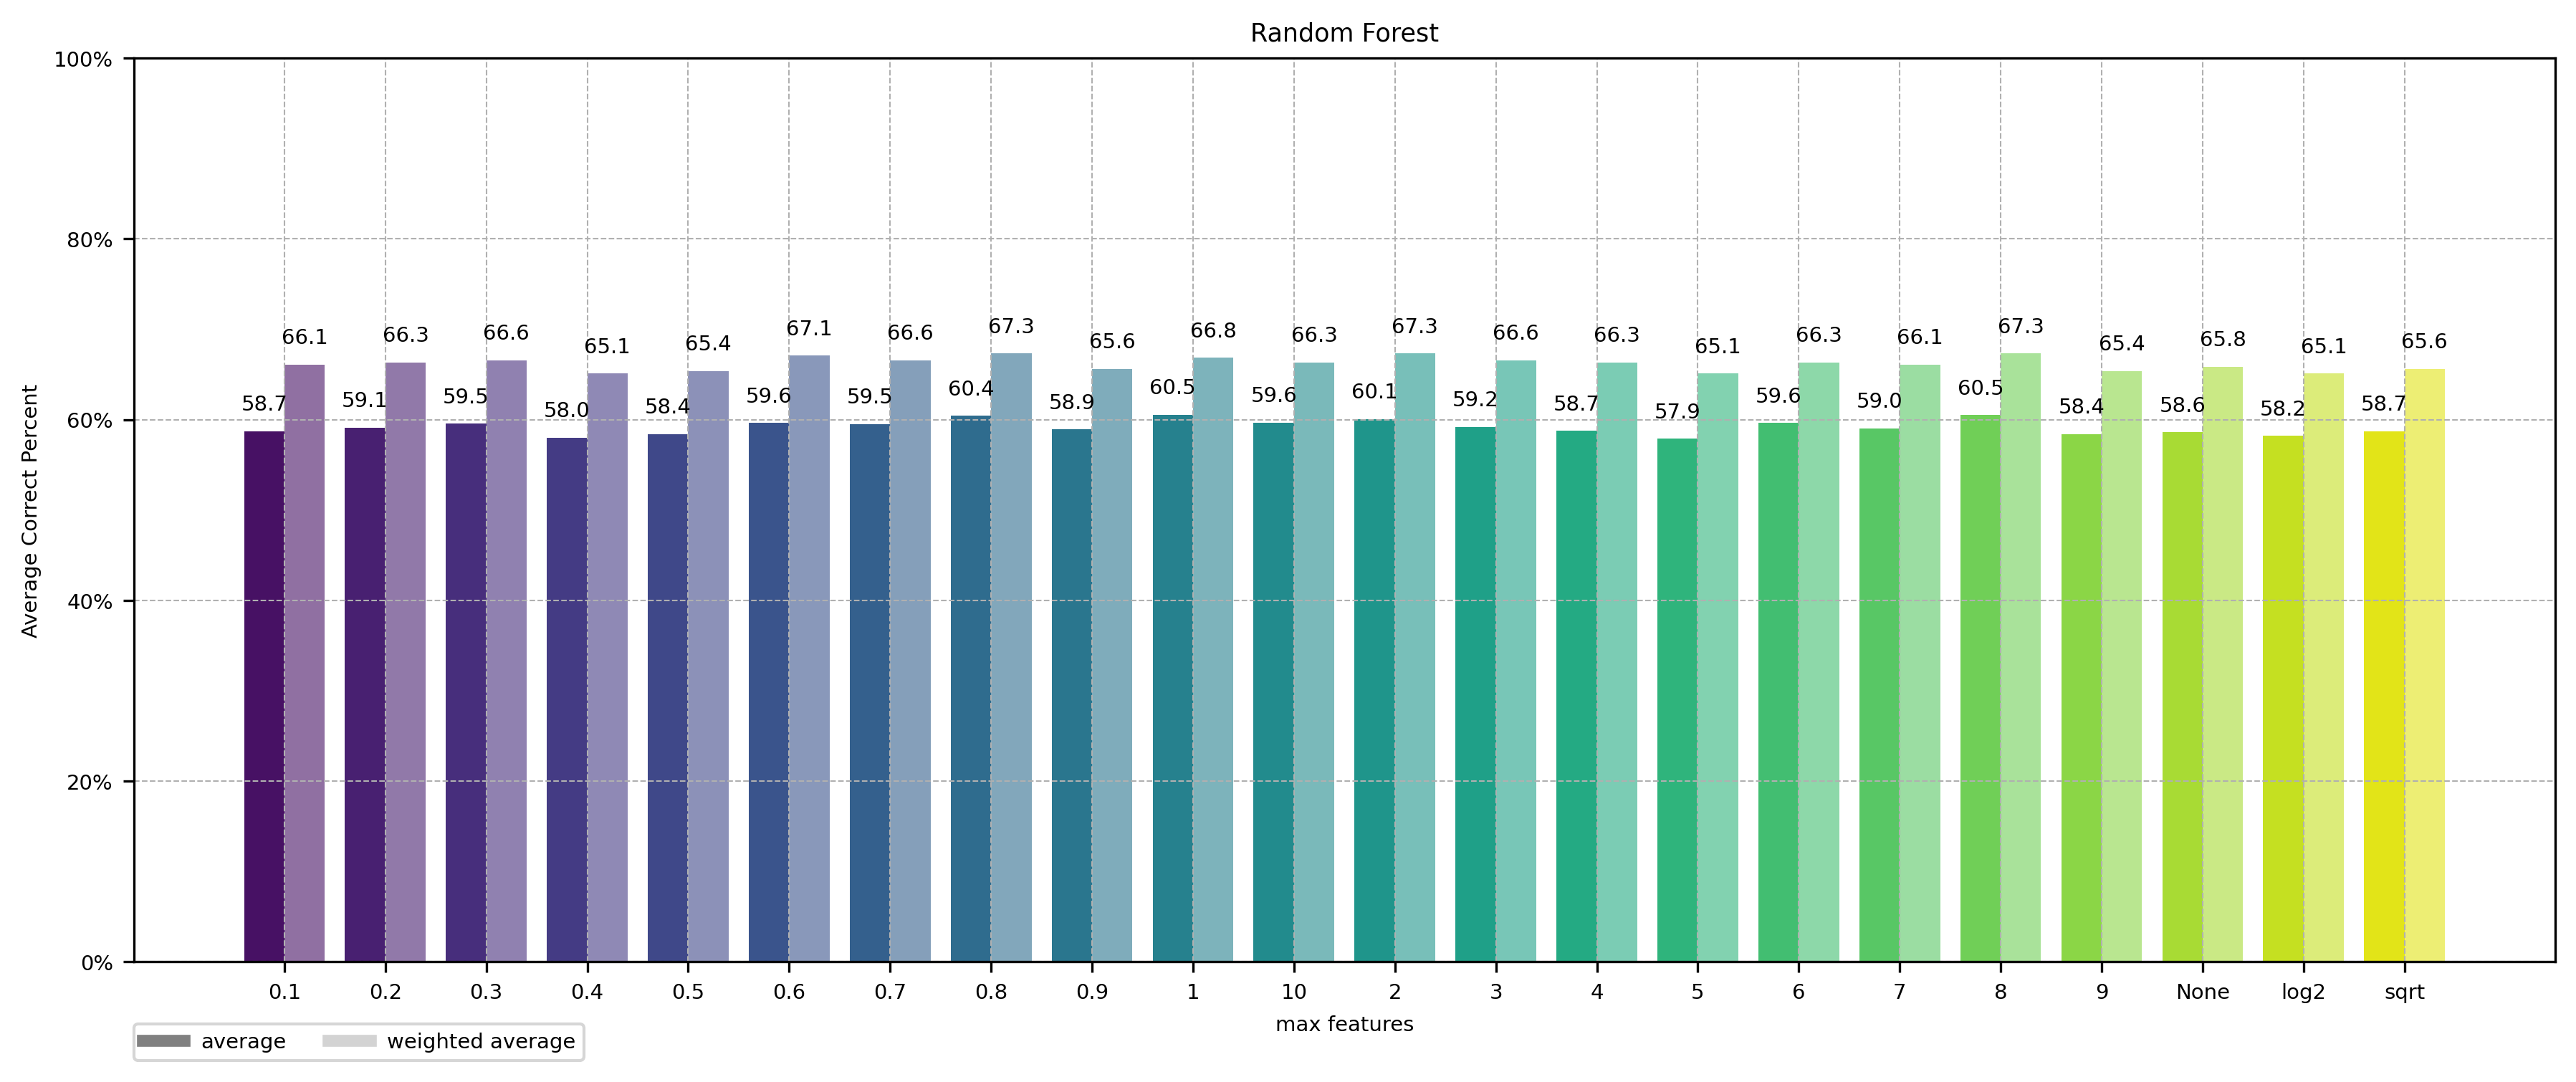
\includegraphics[width=0.8\textwidth]{images/05_best_parameters_random_forest_03.png}
    \caption{Vergleich der Parameter des Random Forest Algorithmus in Abhängigkeit der Anzahl der Messungen}
    \label{fig:05_best_parameters_random_forest_03}
\end{figure}

In Abbildung \ref{fig:05_best_parameters_random_forest_03} sind die durchschnittlichen Genauigkeiten der Parameter für den Random Forest Algorithmus dargestellt. Wie zu erkennen ist, hat die Wahl der Anzahl an Features keinen signifikanten Einfluss auf die Genauigkeit der Raumvorhersagen. Der Mittelwert gewichteten Durchschnitt liegt dabei bei 66,19 \% und bei den ungewichteten Durchschnitten bei 59,15 \%. Die besten Ergebnisse - auch wenn nur mit geringem Abstand - konnten für die Werte \texttt{max\_features = 0,8} (entspricht 80 \% der Features), \texttt{max\_features = 2} und \texttt{max\_features = 8} erzielt werden. Aus diesem Grund wurden für die weiteren Untersuchungen die Werte \texttt{max\_features = 0,8}, \texttt{max\_features = 2} und \texttt{max\_features = 8} ausgewählt.

\section{Untersuchungen des Einflusses verschiedener Datenaufbereitungsmethoden} \label{datenaufbereitung}

In dem folgenden Kapitel werden verschiedene Strategien zur Aufbereitung der Daten untersucht. Dafür wurde jede dieser Strategien in der API-Route \texttt{/measurements/predict} implementiert und kann über die Parameter dieses Endpunktes ausgewählt werden. Für die Analyse dieser Strategien wurde die in Kapitel \ref{testanwendung} vorgestellte Anwendung verwendet.

\subsubsection{Strategien zum Umgang mit fehlenden Werten} \label{strategien}

Im ersten Schritt der Datenaufbereitung wurde untersucht, wie sich verschiedene Strategien zum Umgang mit fehlenden Werten auf die Genauigkeit der Algorithmen auswirken.

Für die Erstellung der \gls{knn}-, \gls{svm}- und Random-Forest-Modelle wurden die Trainingsdaten in Form einer Matrix übergeben, in der für jeden Raum und jeden Router die RSSI-Werte aufgeführt sind. Da jedoch in der Realität nicht in jedem Raum dieselben Router empfangen werden und die Modelle nicht mit fehlenden Werten umgehen können, ist eine Aufbereitung dieser Daten erforderlich. Hierfür wurden verschiedene Strategien entwickelt:

\begin{enumerate}
    \item \textbf{Strategie -100:} Fehlenden Werten wird der Wert -100 dBm zugewiesen. Dieser Wert wurde gewählt, da das der kleinstmögliche RSSI-Wert ist (siehe Kapitel \ref{rssi}). Diese Strategie simuliert, dass der Router zwar erfasst wurde, aber nur ein sehr schwaches Signal gesendet hat.
    \item \textbf{Strategie use\_received:} Fehlende Werte werden durch den entsprechenden Wert in den Testdaten ersetzt. Diese Methode wurde gewählt, weil bei nicht vorhandenen Routern die Distanz null ist und diese somit beim \gls{knn}-Algorithmus ignoriert werden.
    \item \textbf{Strategie zero:} Fehlende Werte werden durch null ersetzt.
\end{enumerate}

In Abbildung \ref{fig:06_handle_missing_values_strategy_02} ist die Genauigkeit der Algorithmen in Abhängigkeit von der gewählten Strategie zum Umgang mit fehlenden Werten dargestellt. Es zeigt sich, dass die zweite Strategie bei \gls{knn} und Random Forest zu keiner Verbesserung der Ergebnisse führt und auch bei zunehmender Anzahl an Messungen keine Tendenz zu besseren Ergebnissen erkennbar ist. Auffällig bei diesen beiden Modellen ist, dass bei der \texttt{use\_received} Strategie eine leichte Steigerung der Genauigkeit bei 11 Messungen pro Raum zu beobachten ist, während die anderen beiden Strategien bei dieser Anzahl an Messungen eine entgegengesetzte Entwicklung zeigen. Die \texttt{use\_received} Strategie konnte bei 11 Messungen pro Raum zum Teil bessere Ergebnisse erzielen als die anderen beiden Strategien. Im direkten Vergleich der ersten und dritten Strategie für \gls{knn} und Random Forest ist zu erkennen, dass die Zuweisung von -100 dBm bei fehlenden Werten zu besseren Ergebnissen führt als die Ersetzung durch 0 dBm, auch wenn die Unterschiede gering sind.

Bei dem \gls{svm} Algorithmus zeigt sich im Gegensatz zu den anderen beiden Modellen, dass die Genauigkeit bei der zweiten Strategie mit zunehmender Anzahl an Messungen tendenziell steigt. Dennoch sind auch hier die anderen beiden Strategien überlegen.

\begin{figure}[H]
    \centering
    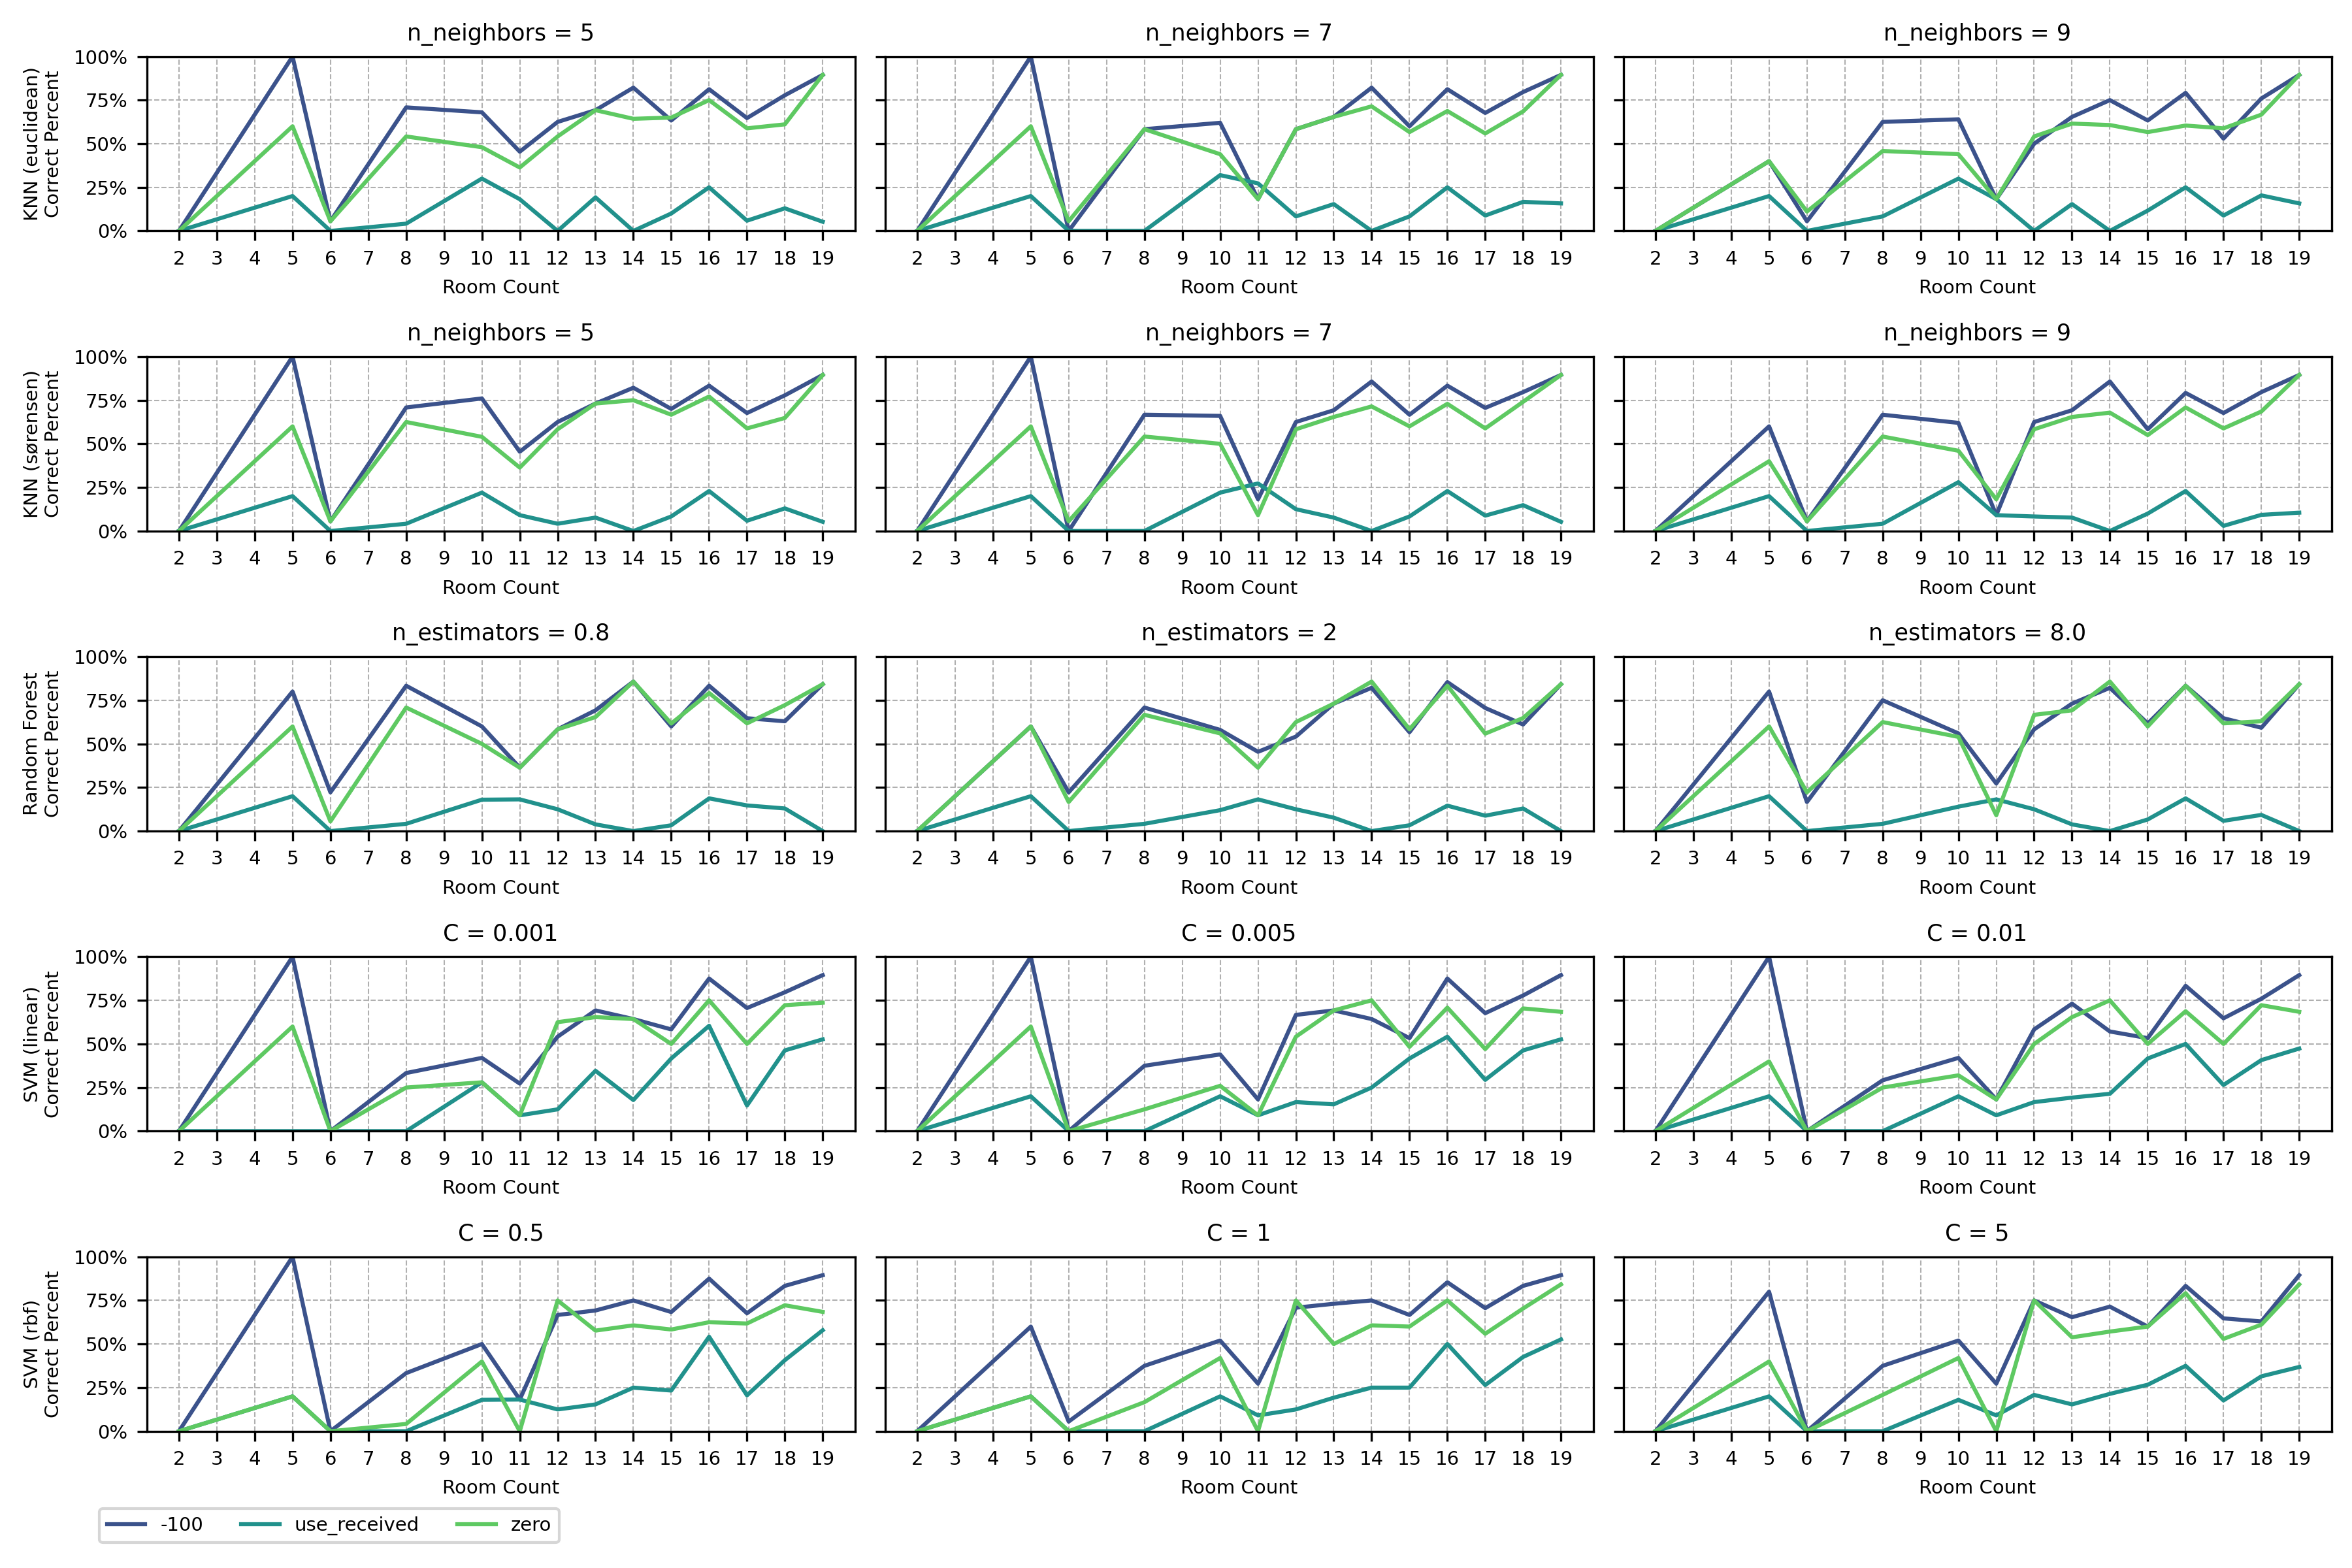
\includegraphics[width=0.8\textwidth]{images/06_handle_missing_values_strategy_02.png}
    \caption{Vergleich der Genauigkeit in Abhängigkeit der Strategie zum Umgang mit fehlenden Werten}
    \label{fig:06_handle_missing_values_strategy_02}
\end{figure}

Wie in Abbildung \ref{fig:06_handle_missing_values_strategy_03} zu erkennen ist, führt die erste Strategie in allen Fällen zu den besten Ergebnissen, wenn die durchschnittliche Genauigkeit betrachtet wird. Aus diesem Grund werden in den weiteren Untersuchungen fehlende Werte durch -100 dBm ersetzt.

\begin{figure}[H]
    \centering
    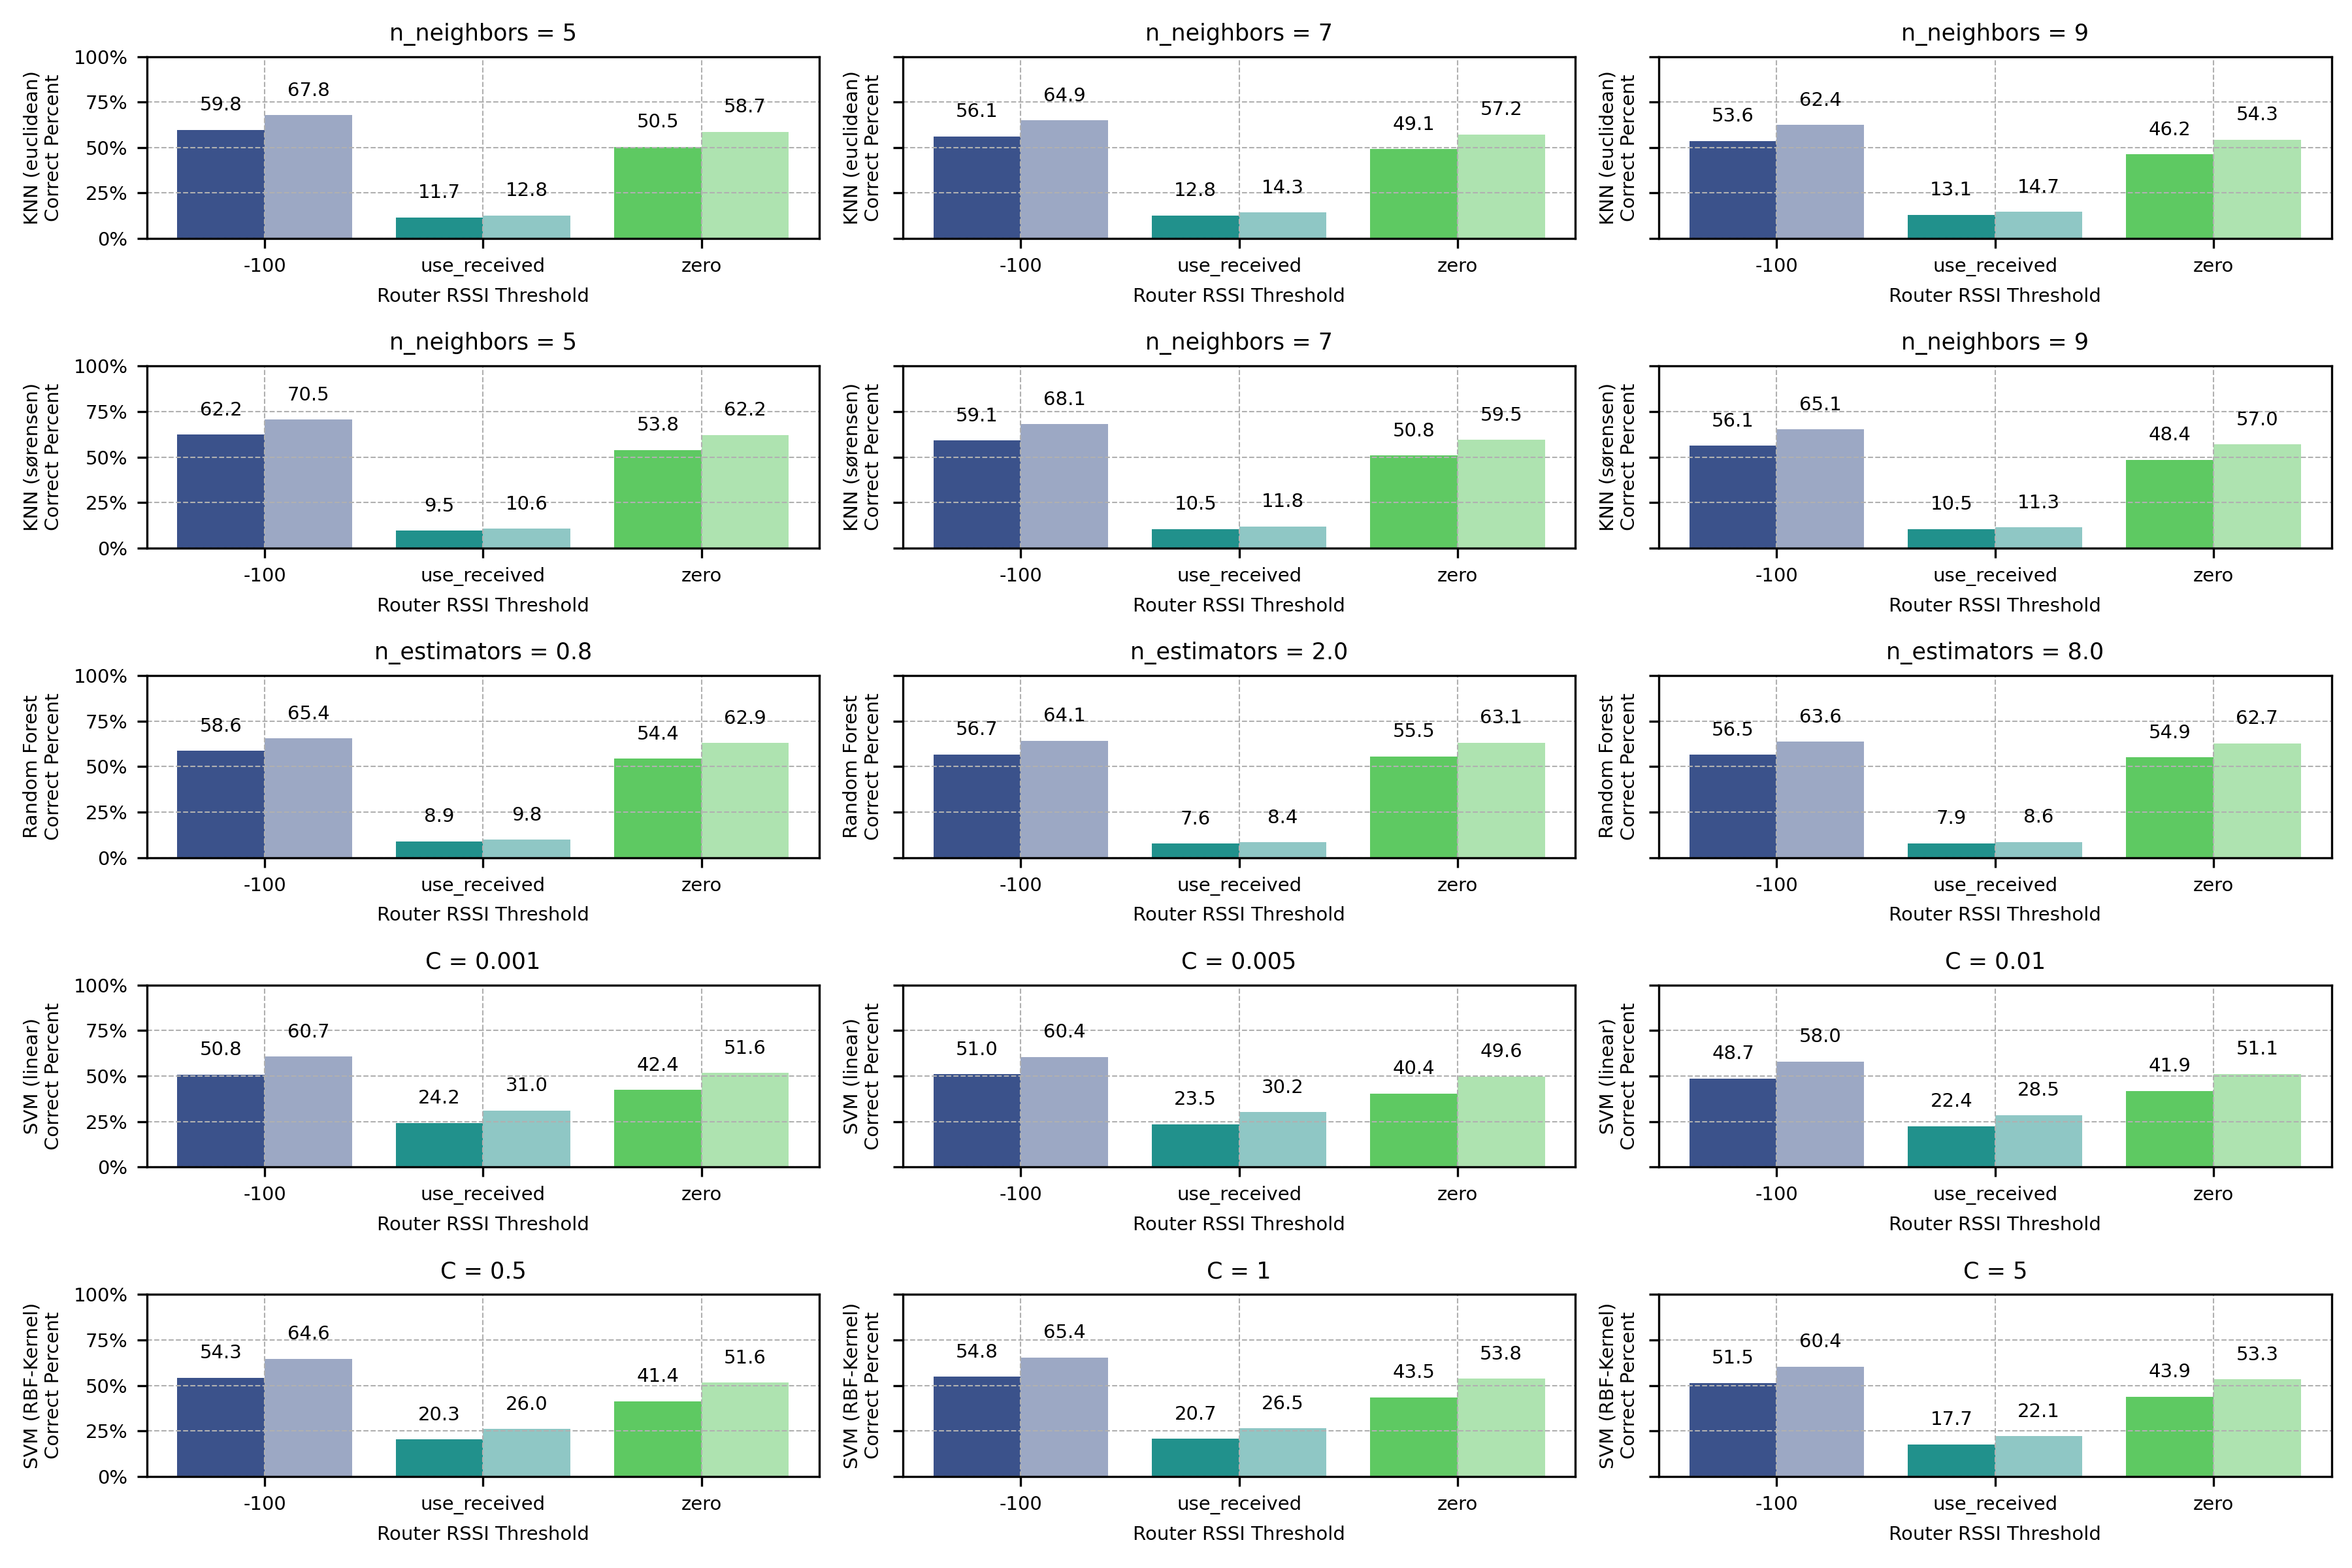
\includegraphics[width=0.8\textwidth]{images/06_handle_missing_values_strategy_03.png}
    \caption{Vergleich der durchschnittlichen Genauigkeit in Abhängigkeit der Strategie zum Umgang mit fehlenden Werten}
    \label{fig:06_handle_missing_values_strategy_03}
\end{figure}

\subsubsection{Einfluss der verwendeten Router}

Im zweiten Schritt der Datenaufbereitung wird untersucht, ob die Auswahl der Router einen Einfluss auf die Genauigkeit der Modelle hat. Der Gedanke hinter diesem Aufbereitungsschritt ist, dass nicht alle empfangenen Access Points ortsgebunden sind (z. B. Hotspots von mobilen Endgeräten) und somit einen negativen Einfluss auf die korrekte Raumvorhersage haben können. Deswegen könnte es von Vorteil sein, wenn nur die Access Points der eduroam-Infrastruktur (\textit{eduroam}, \textit{HowToUseEduroam} und \textit{Gast@HTW}) für die Vorhersagen verwendet werden.

Aus diesem Grund wird in diesem Aufbereitungsschritt untersucht, wie sich die Genauigkeit der Modelle verhält, wenn nur die Router der \textit{eduroam}-Infrastruktur für die Vorhersagen verwendet werden.

Wie in Abbildung \ref{fig:07_router_selection_02} zu erkennen ist, sind die Ergebnisse für alle Modelle und alle Parameterkonfigurationen - mit Ausnahme von den Ergebnissen bei 5 Messungen pro Raum - fast identisch. Dies deutet darauf hin, dass die Auswahl der Router bei diesen Daten keinen signifikanten Einfluss auf die Genauigkeit der Modelle hat und dass in dem Raum in dem 5 Messungen durchgeführt wurden die nicht-\textit{eduroam} Access Points einen besonders großen Einfluss haben bzw. die \textit{eduroam} Access-Points nicht aussagekräftig genug sind. Für die weiteren Untersuchungen wurde sich daher dafür entschieden nur die \textit{eduroam} Router zu betrachten, da bei diesen Routern davon ausgegangen werden kann, dass diese ihre Position nicht verändern und die Unterschiede - abgesehen von dem Raum mit 5 Messungen - minimal sind.

\begin{figure}[H]
    \centering
    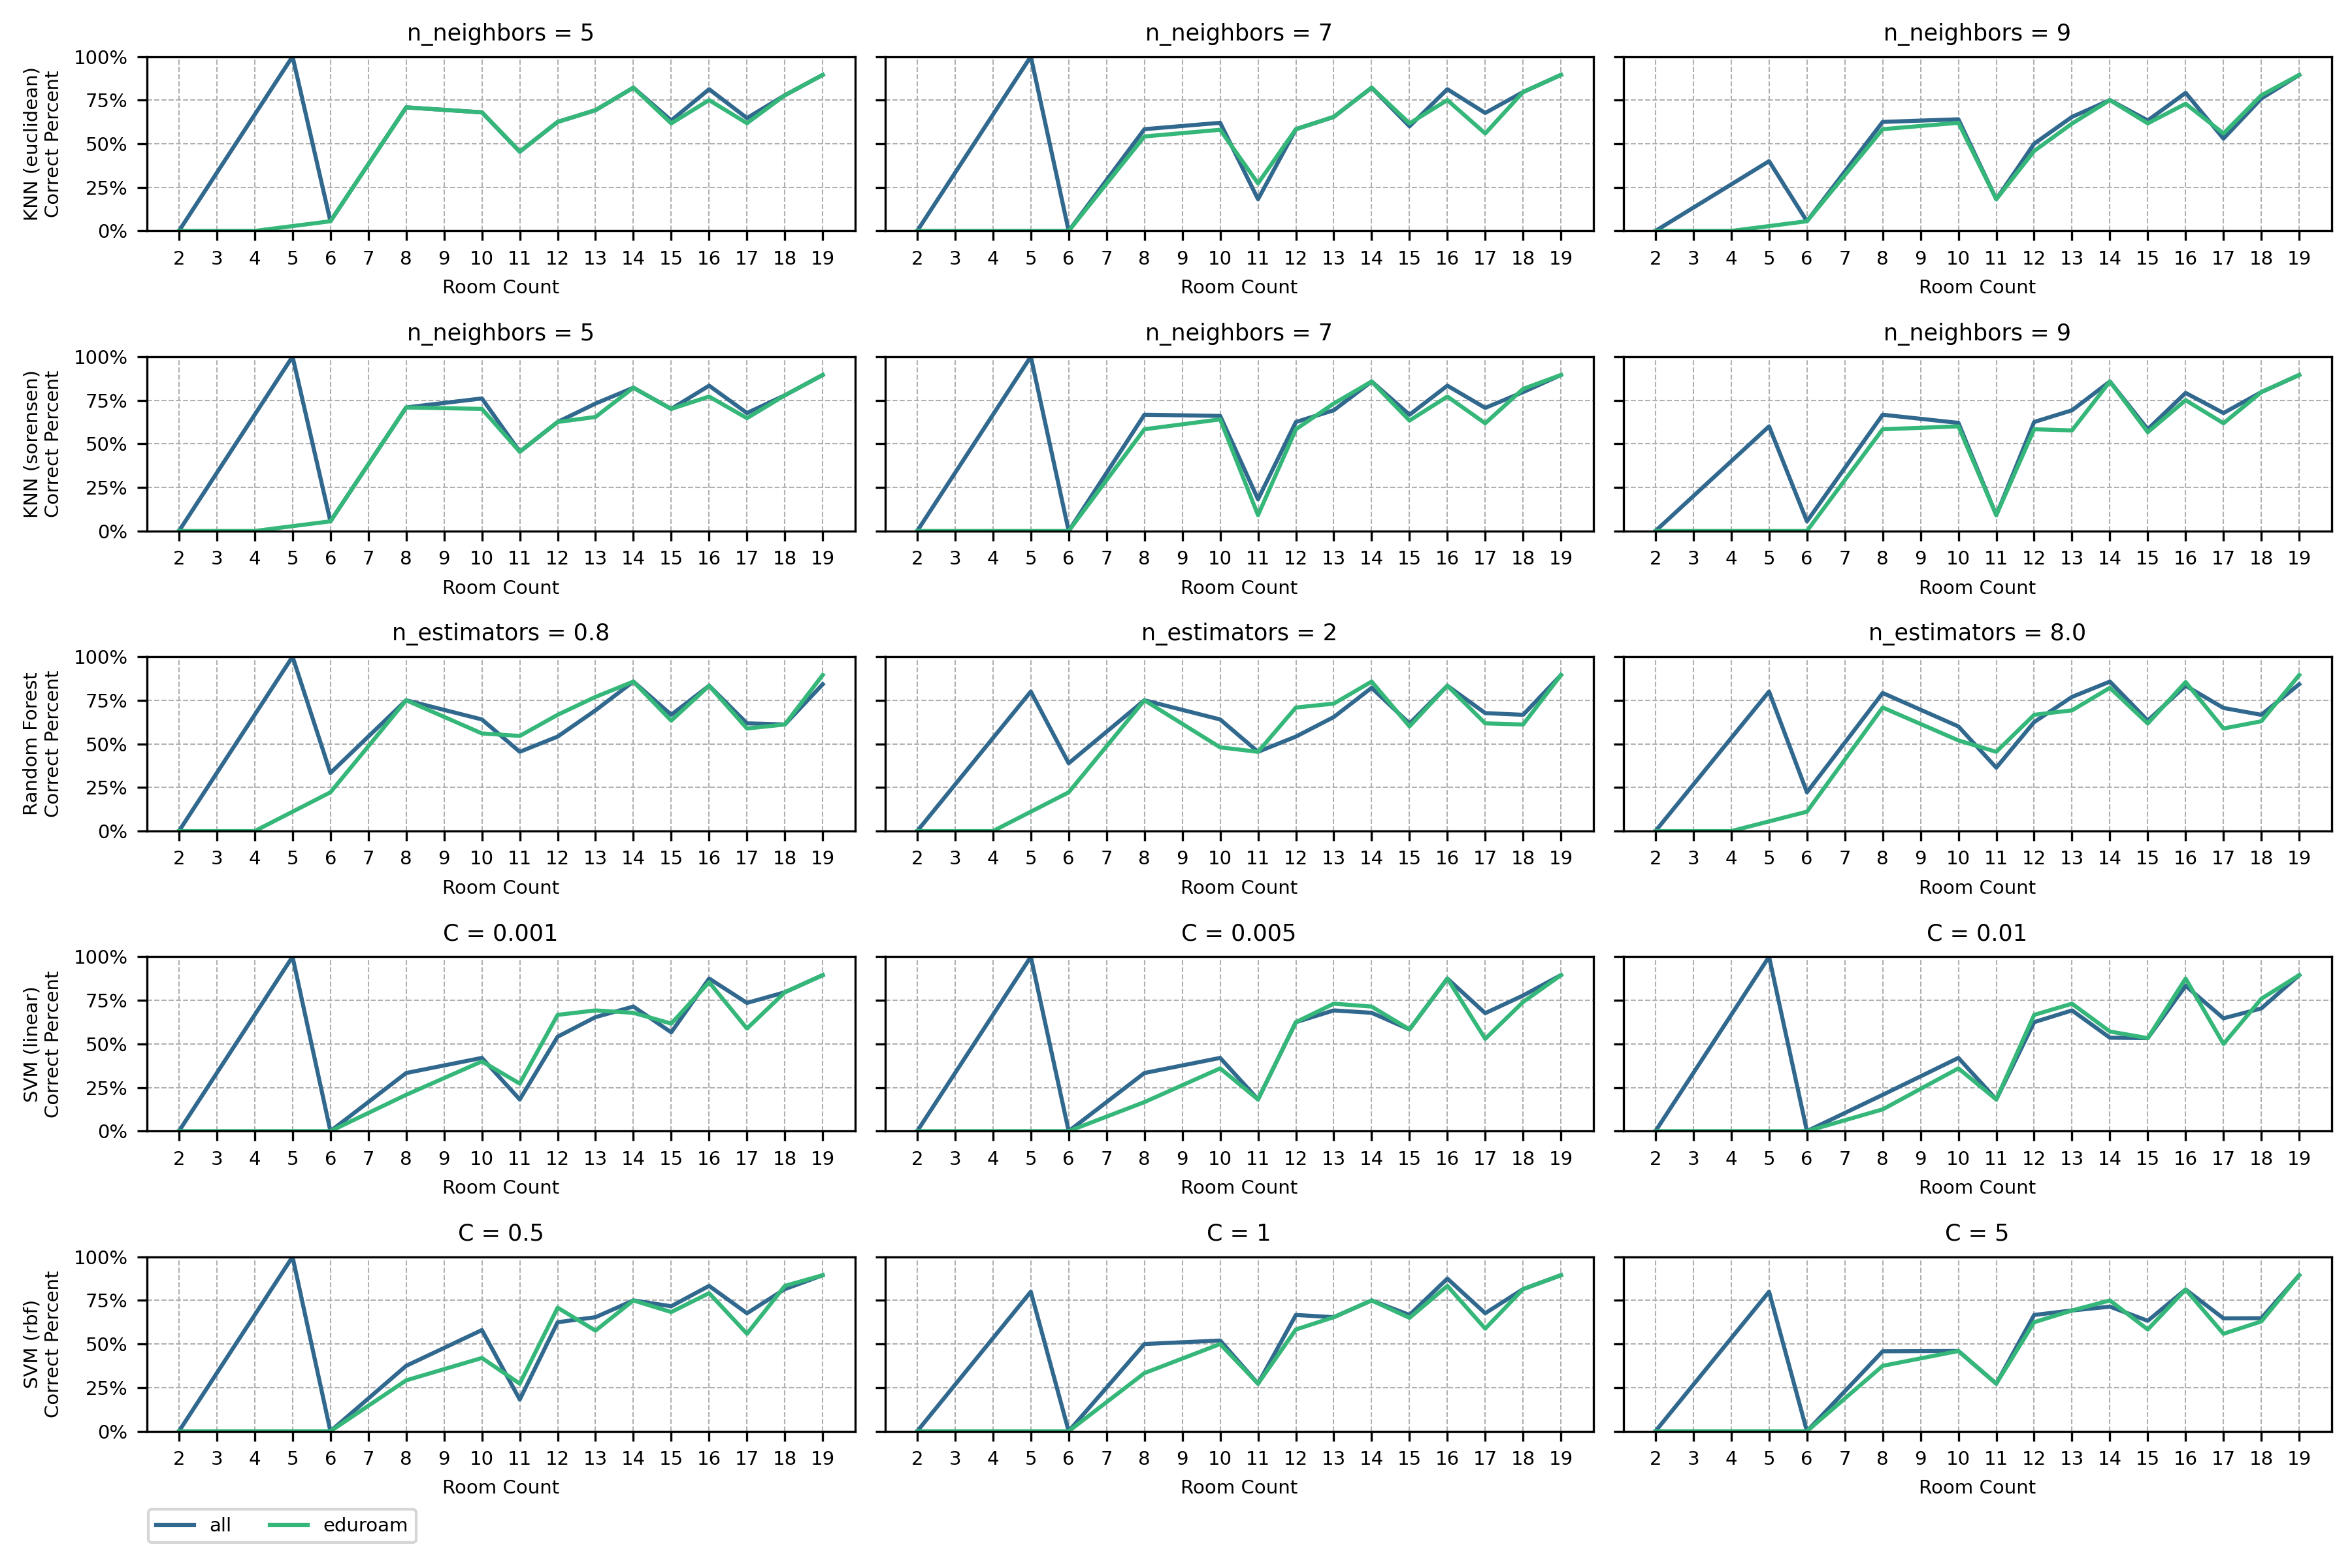
\includegraphics[width=0.8\textwidth]{images/07_router_selection_02.png}
    \caption{Vergleich der Genauigkeit in Abhängigkeit der Strategie zur Auswahl der Router}
    \label{fig:07_router_selection_02}
\end{figure}

\subsubsection{Filterung von RSSI-Werten}
\subsubsection{Berücksichtigung nur häufig auftretender Router}

Im dritten Schritt der Datenaufbereitung wird analysiert, ob die Genauigkeit verbessert werden kann, wenn nur Access Points berücksichtigt werden, die in mehreren Messungen eines Raums erfasst wurden. Die zugrunde liegende Annahme ist, dass Router, die häufiger in einem Raum empfangen werden, repräsentativer sind als solche, die nur selten erfasst werden. Aus diesem Grund wurden verschiedene Schwellenwerte getestet, die den Prozentsatz der berücksichtigten Router angeben. Dabei wurde unter anderem die bisherige Einstellung, bei der alle Router einbezogen werden, sowie die Schwellenwerte von 25 \%, 50 \% und 75 \% untersucht. Das bedeutet, dass beispielsweise nur die Router berücksichtigt werden, die in mindestens 25 \% der Messungen eines Raums vorhanden sind.

\begin{figure}[H]
    \centering
    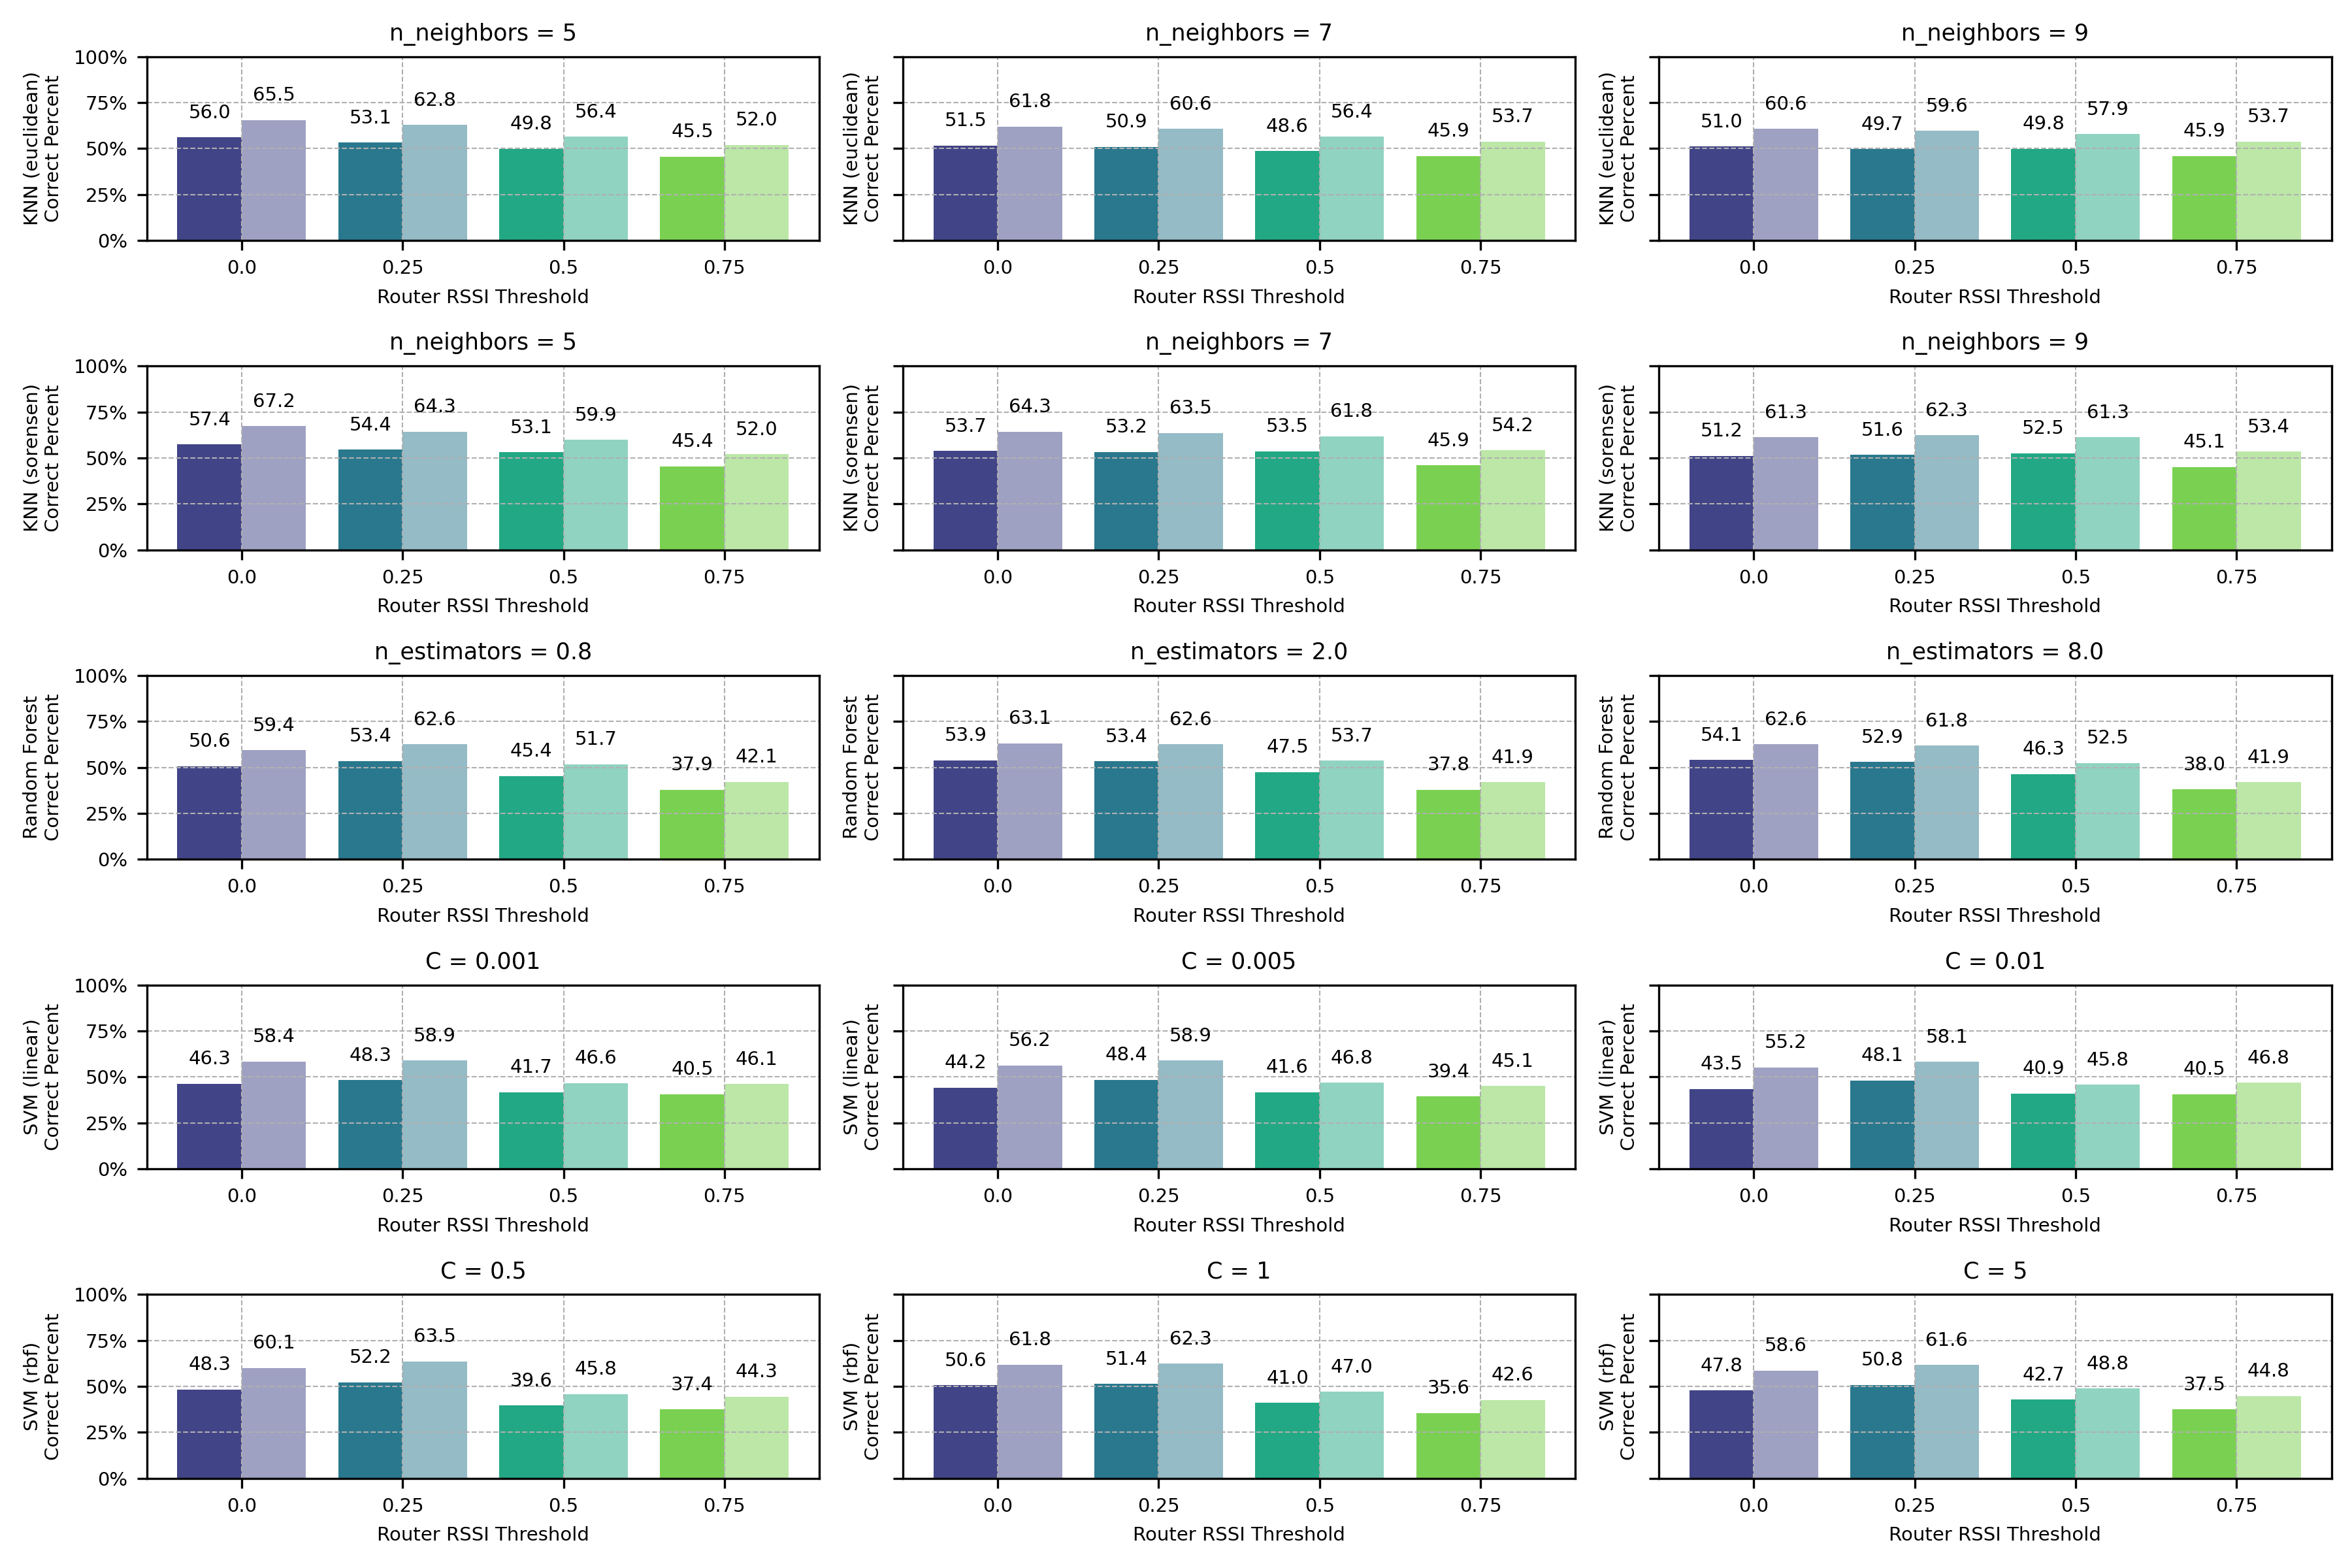
\includegraphics[width=0.8\textwidth]{images/08_router_presence_threshold_03.png}
    \caption{Vergleich der durchschnittlichen Genauigkeit in Abhängigkeit des Schwellenwerts für die Anzahl der Messungen eines Routers}
    \label{fig:08_router_presence_threshold_03}
\end{figure}

Wie in Abbildung \ref{fig:08_router_presence_threshold_03} zu sehen ist, sinkt die Genauigkeit bei beiden \gls{knn}-Modellen, mit Ausnahme der Sørensen Distanzmetrik für den Wert k = 9, sowie bei dem Random Forest Modell, mit Ausnahme der Werte für \texttt{max\_features = 0,8}, mit steigendem Schwellenwert. Bei dem \gls{knn} Algorithmus unter Verwendung der Sørensen Distanz und k = 9 und dem Random Forest Algorithmus mit \texttt{max\_features = 0,8} zeigt der Schwellenwert von 25 \% jedoch eine etwas bessere Genauigkeit als der Schwellenwert von 0 \%. Bei dem \gls{svm} Modell zeigt sich unabhängig vom Kernel, dass die Ergebnisse bei einem Schwellenwert von 25 \% bei allen Parametern am besten sind und die Genauigkeit mit zu- und abnehmendem Schwellenwert sinkt. Aus diesem Grund werden für das \gls{knn}- und Random Forest-Modell bei den folgenden Untersuchungen alle Router berücksichtigt (Schwellenwert von 0 \%) und bei den \gls{svm}-Modellen nur die Access Points, die in mindestens 25 \% der Messungen eines Raums vorhanden sind.

\subsubsection{Ausschluss von Routern mit schwachem Signal}

Im vierten Schritt der Datenaufbereitung wird untersucht, ob die Genauigkeit der Modelle verbessert werden kann, indem Router mit einem schwachen Signal ausgeschlossen werden. Die Annahme dahinter ist, dass Router mit einem schwachen Signal weniger aussagekräftig sind als Router mit einem stärkeren Signal. Aus diesem Grund wurden verschiedene Schwellenwerte getestet, die den minimalen RSSI-Wert angeben, den ein Router haben muss, um berücksichtigt zu werden. Dabei wurden die Schwellenwerte von -100 dBm, -90 dBm, -80 dBm, -70 dBm, -60 dBm, -50 dBm und -40 dBm untersucht. Diese Idee basiert auf dem Paper \textit{Comprehensive analysis of distance and similarity measures for Wi-Fi fingerprinting indoor positioning systems}.\myfootcite{TorresSospedra2015WiFi}{S. 9272}

% \begin{itemize}
%     \item Idee: sehr kleine RSSI Werte werden ignoriert/so getan, als wäre die bei der Messung nicht dabei
%     \item Gedanke dahiner: Router mit größeren RSSI-Werten sind aussagekräftiger und sollten dadurch mehr Einfluss haben
%     \item Ergebnis: Bei allen Algorithmen ist -100 am besten -> Router mit geringen RSSI-Werten haben einen größeren Einfluss als vermutet
%     \item Idee ist nicht von mir, sondern kommt aus dem Paper: Quelle: Comprehensive analysis of distance and similarity measures for Wi-Fi fingerprinting indoor positioning systems
%     \item Die Thresholds sind: -100, -90, -80, -70, -60, -50, -40
% \end{itemize}

\begin{figure}[H]
    \centering
    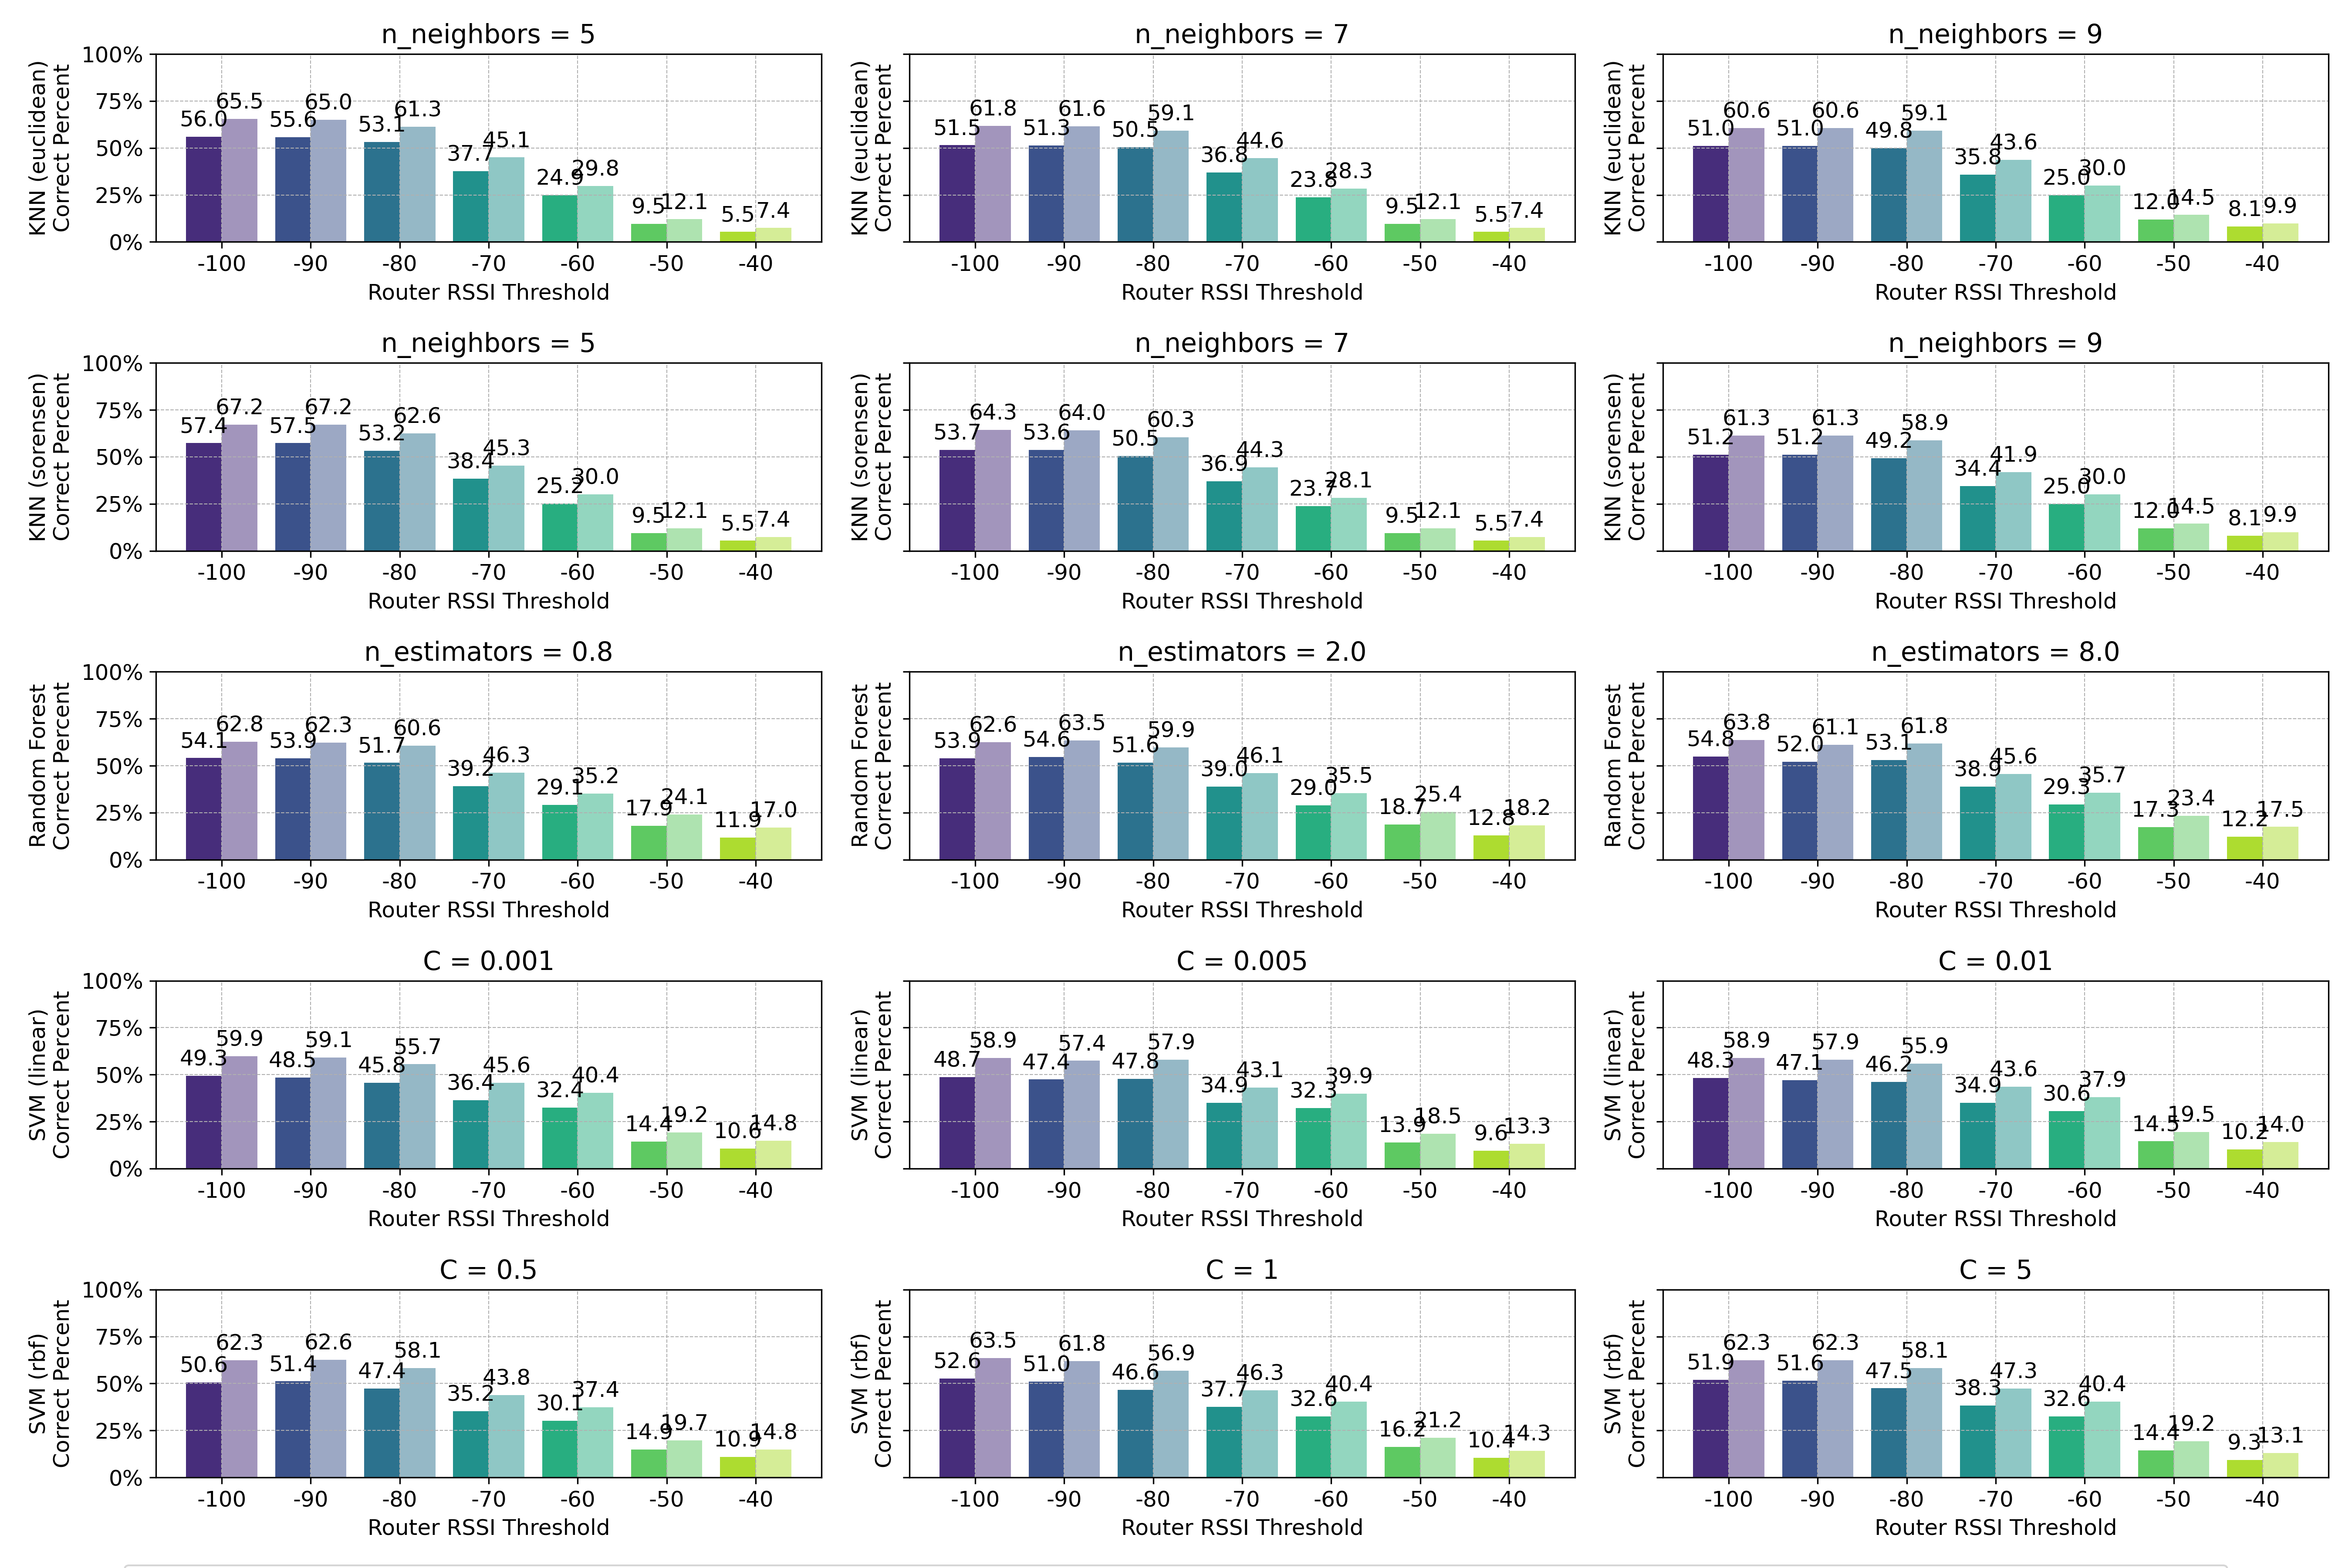
\includegraphics[width=0.8\textwidth]{images/09_router_rssi_threshold_03.png}
    \caption{Vergleich der durchschnittlichen Genauigkeit in Abhängigkeit des Schwellenwerts für die Mindestsignalstärke eines Routers}
    \label{fig:09_router_rssi_threshold_03}
\end{figure}

Wie in Abbildung \ref{fig:09_router_rssi_threshold_03} zu erkennen ist, führt die Ignorierung von Routern mit einem schwachen Signal zu keiner Verbesserung der Ergebnisse und die Genauigkeit der Vorhersagen nimmt in den meisten Fällen - abgesehen von ein paar Ausnahmen - linear ab. Bei den Ausnahmen (\gls{svm} mit RBF-Kernal und C = 0,5, Random Forest mit einer maximalen Anzahl von 2 Features und \gls{knn} mit der Sørensen-Distanz und k = 5) zeigt sich, dass die Genauigkeit bei einem Schwellenwert von -90 dBm leicht besser ist als die Genauigkeit bei einem Schwellenwert von -100 dBm. Insgesamt ist jedoch zu erkennen, dass die Ergebnisse bei einem Schwellenwert von -100 dBm am besten sind. Aus diesem Grund wird für die weiteren Untersuchungen ein Schwellenwert von -100 dBm verwendet.

\subsubsection{Skalierung von RSSI-Werten}

Im fünften Schritt der Datenaufbereitung wird untersucht, ob die Skalierung der RSSI-Werte die Genauigkeit der Modelle verbessern kann. Die Idee hinter der Werteskalierung stammt aus dem Paper \textit{Comprehensive analysis of distance and similarity measures for Wi-Fi fingerprinting indoor positioning systems} und basiert auf der Erkenntnis, dass die RSSI-Werte nicht linear verteilt sind (siehe Kapitel \ref{pfadverlustmodell}). Dafür werden wie in dem Paper beschrieben drei verschiedene Skalierungsmethoden implementiert und mit den bisher nicht skalierten Werten verglichen.\myfootcite{TorresSospedra2015WiFi}{S. 9269}

Die drei Skalierungsmethoden sind:

\begin{enumerate}
    \item \textbf{Lineare Normalisierung}
    \item \textbf{Exponentielle Skalierung}
    \item \textbf{Potenzierte Skalierung}
\end{enumerate}

% \subsubsection{Formeln}

% % Quelle XX: Comprehensive analysis of distance and similarity measures for Wi-Fi fingerprinting indoor positioning systems

% Die Idee hinter der Werteskalierung stammt aus der Quelle XX und basiert auf der Erkenntnis, dass die RSSI-Werte nicht linear verteilt sind. Durch eine geeignete Skalierung kann der Zusammenhang zwischen Entfernung und RSSI-Wert besser abgebildet werden. In der vorliegenden Arbeit wurden drei Skalierungsmethoden aus der Quelle XX implementiert und verglichen.

Grundlage jeder Skalierung ist die positive Darstellung der Werte. Hierfür wird jeder Wert in den Trainings- und Testdaten mit dem niedrigsten gemessenen RSSI-Wert minus 1 dBm (\(\text{min}\)) subtrahiert:

\begin{equation}
    \text{Positiv}_i(x) = \text{RSS}_i - (\text{min})
    \label{eq:positive_values_representation}
\end{equation}

Durch diese Skalierung werden alle RSSI-Werte positiv dargestellt und der niedrigste Wert ist 1 dBm.

\textbf{Lineare Normalisierung:}

Die linear normalisierten Werte werden berechnet mit:

\begin{equation}
    \text{Normiert}_i(x) = \frac{\text{Positiv}_i(x)}{-\text{min}}
    \label{eq:linear_normalized_values}
\end{equation}

und befeinden nach der Skalierung in dem Wertebereich [0, 1].

\textbf{Exponentielle Skalierung:}

Die exponentiell skalierten Werte werden berechnet mit:

\begin{equation}
    \text{Exponential}_i(x) = \frac{\exp\left(\frac{\text{Positiv}_i(x)}{\alpha}\right)}{\exp\left(\frac{-\text{min}}{\alpha}\right)}
    \label{eq:exponential_representation}
\end{equation}

und \(\alpha = 24\).

Die Auswahl dieses Wertes für den Parameter \(\alpha\) basiert auf den Ergebnissen aus dem Paper {Comprehensive analysis of distance and similarity measures for Wi-Fi fingerprinting indoor positioning systems}.\myfootcite{TorresSospedra2015WiFi}{S. 9269}

\textbf{Potenzierte Skalierung:}

Die potenzierten Werte werden unter Verwendung von \(\beta = e\) und der Formel:

\begin{equation}
    \text{Potenziert}_i(x) = \left(\frac{\text{Positiv}_i(x)}{-\text{min}}\right)^{\beta}
    \label{eq:powered_representation}
\end{equation}

berechnet. Diese Auswahl basiert ebenfalls auf den Ergebnissen aus dem Paper \textit{Comprehensive analysis of distance and similarity measures for Wi-Fi fingerprinting indoor positioning systems}.\myfootcite{TorresSospedra2015WiFi}{S. 9269}

In Abbildung \ref{fig:value_scaling_strategies_ignore_10} sind die verschiedenen Skalierungsmethoden dargestellt. Für diese exemplarische Darstellung wurden RSSI-Werte zwischen -100 dBm und -1 dBm in einem Interval von 1 dBm betrachtet.

\begin{figure}[H]
    \centering
    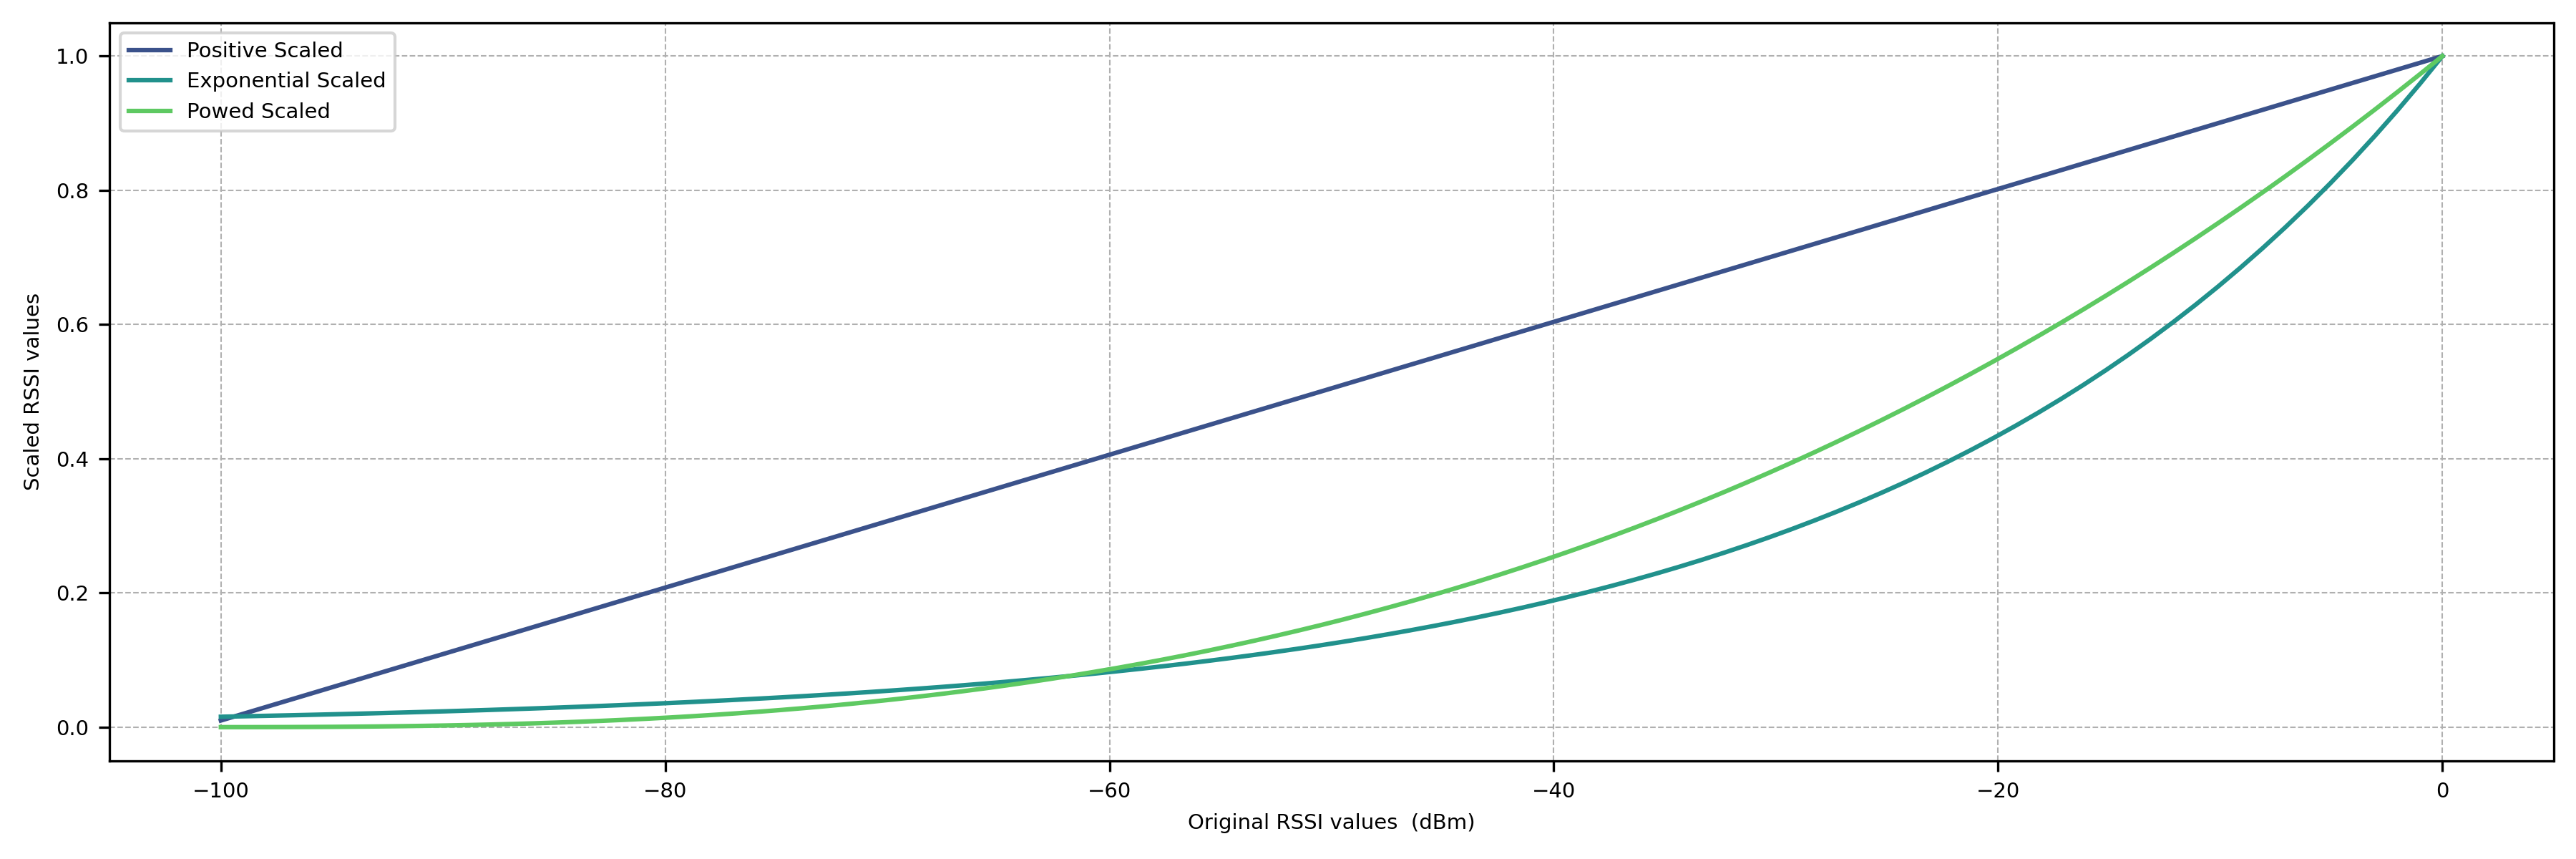
\includegraphics[width=0.8\textwidth]{images/plot_scaling_strategies.png}
    \caption{Darstellung der verschiedenen Skalierungsmethoden}
    \label{fig:value_scaling_strategies_ignore_10}
\end{figure}

Da in dem \gls{knn}-Modell die Distanzen zur Bestimmung der Räume auf den RSSI-Werten basieren und die Skalierung dieser Werte den Wertebereich beeinflusst hat, wird zunächst überprüft, ob die gewählte Gewichtung (\texttt{weights = distance}) weiterhin optimal ist. Dazu wurde der \gls{knn}-Algorithmus mit beiden Gewichtungsfunktionen und beiden Distanzmetriken jeweils mit linearer Normalisierung, exponentieller Skalierung, potenzierter Skalierung und den unskalierten Werten verglichen.

\begin{figure}[H]
    \centering
    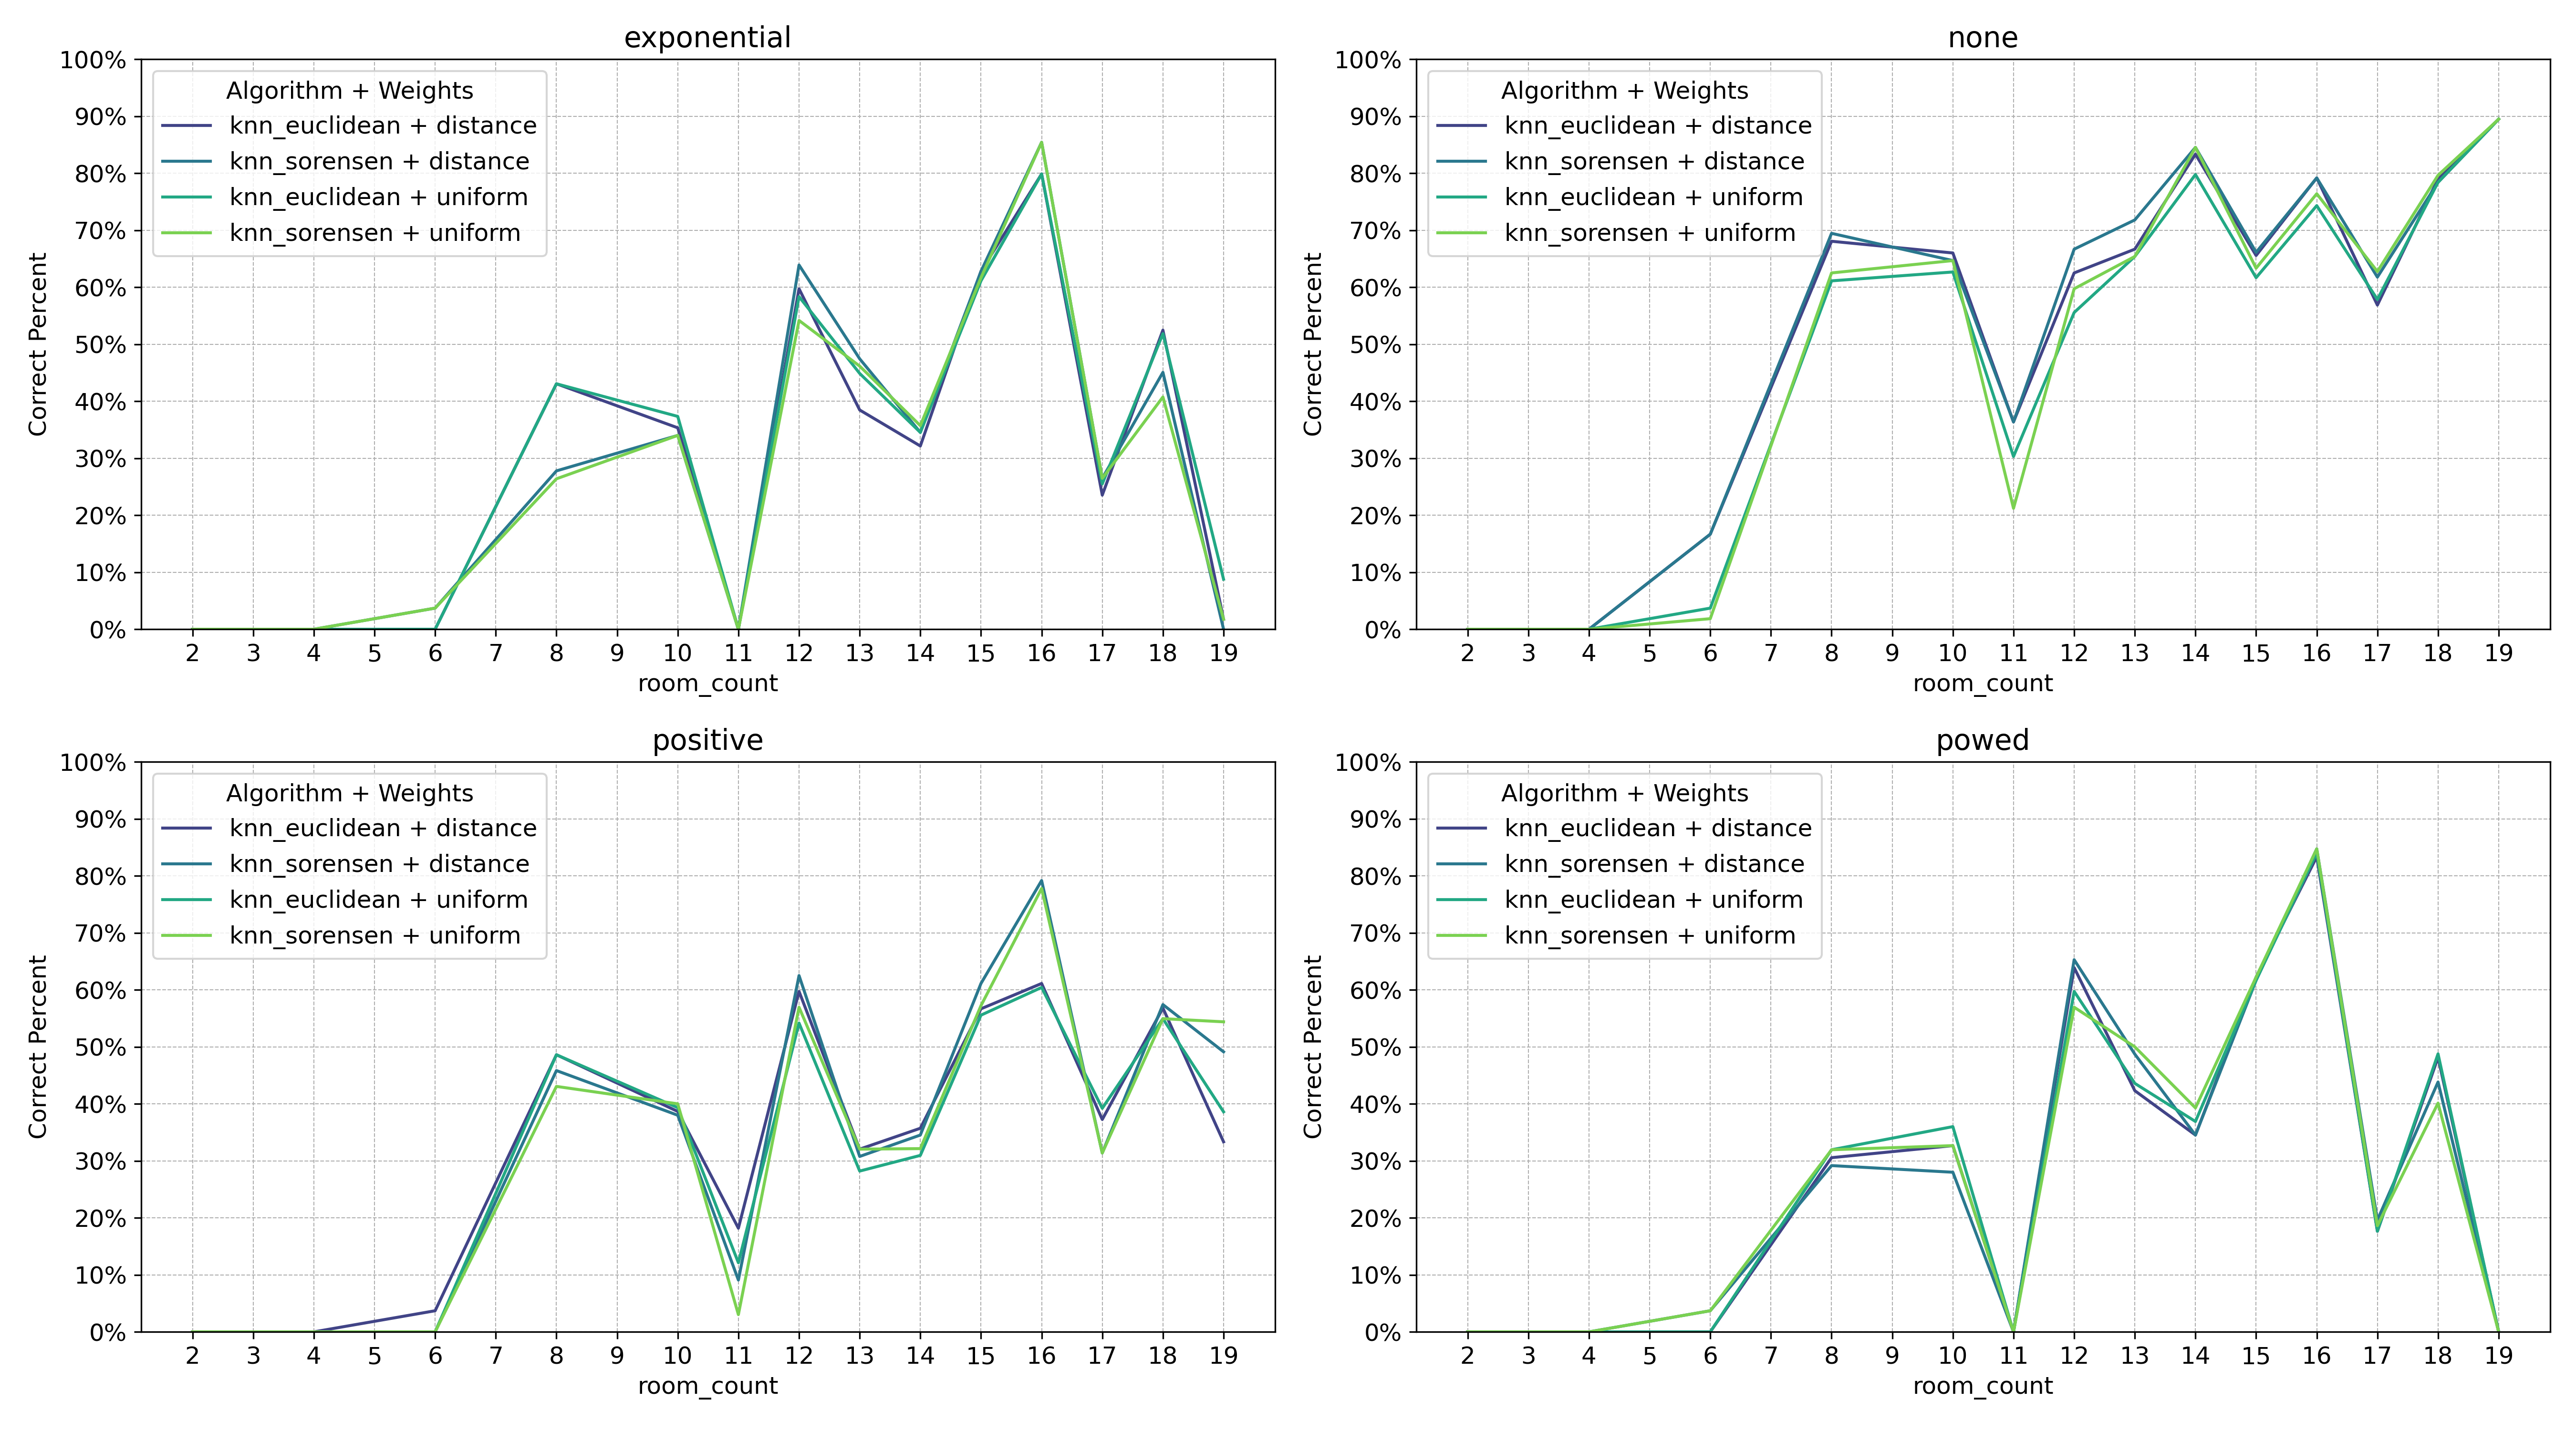
\includegraphics[width=0.8\textwidth]{images/10_knn_weights_value_scaling_strategy_03.png}
    \caption{Vergleich des \gls{knn}-Algorithmus mit den verschiedenen Skalierungsmethoden und beiden Gewichtungsfunktionen}
    \label{fig:10_knn_weights_value_scaling_strategy_03}
\end{figure}

Wie in Abbildung \ref{fig:10_knn_weights_value_scaling_strategy_03} zu erkennen ist, zeigen die Ergebnisse unabhängig von der gewählten Distanzmetrik und der Gewichtungsfunktion einen ähnlichen Verlauf innerhalb jeder Skalierungsstrategie. Auffällig ist jedoch, dass bei der exponentiellen und der potenzierten Skalierung die Genauigkeit in Räumen mit mehr als 16 Messungen deutlich abnimmt, wobei der Rückgang bei der potenzierten Skalierung weniger stark ausgeprägt ist. Zudem gibt es leichte Unterschiede zwischen den Distanzmetriken: Bei der exponentiellen Skalierung schneidet die Sørensen-Distanz in Räumen mit 8 Messungen schlechter ab und bei der positiven Skalierung in Räumen mit 16 Messungen, jeweils im Vergleich zur euklidischen Distanz.

\begin{figure}[H]
    \centering
    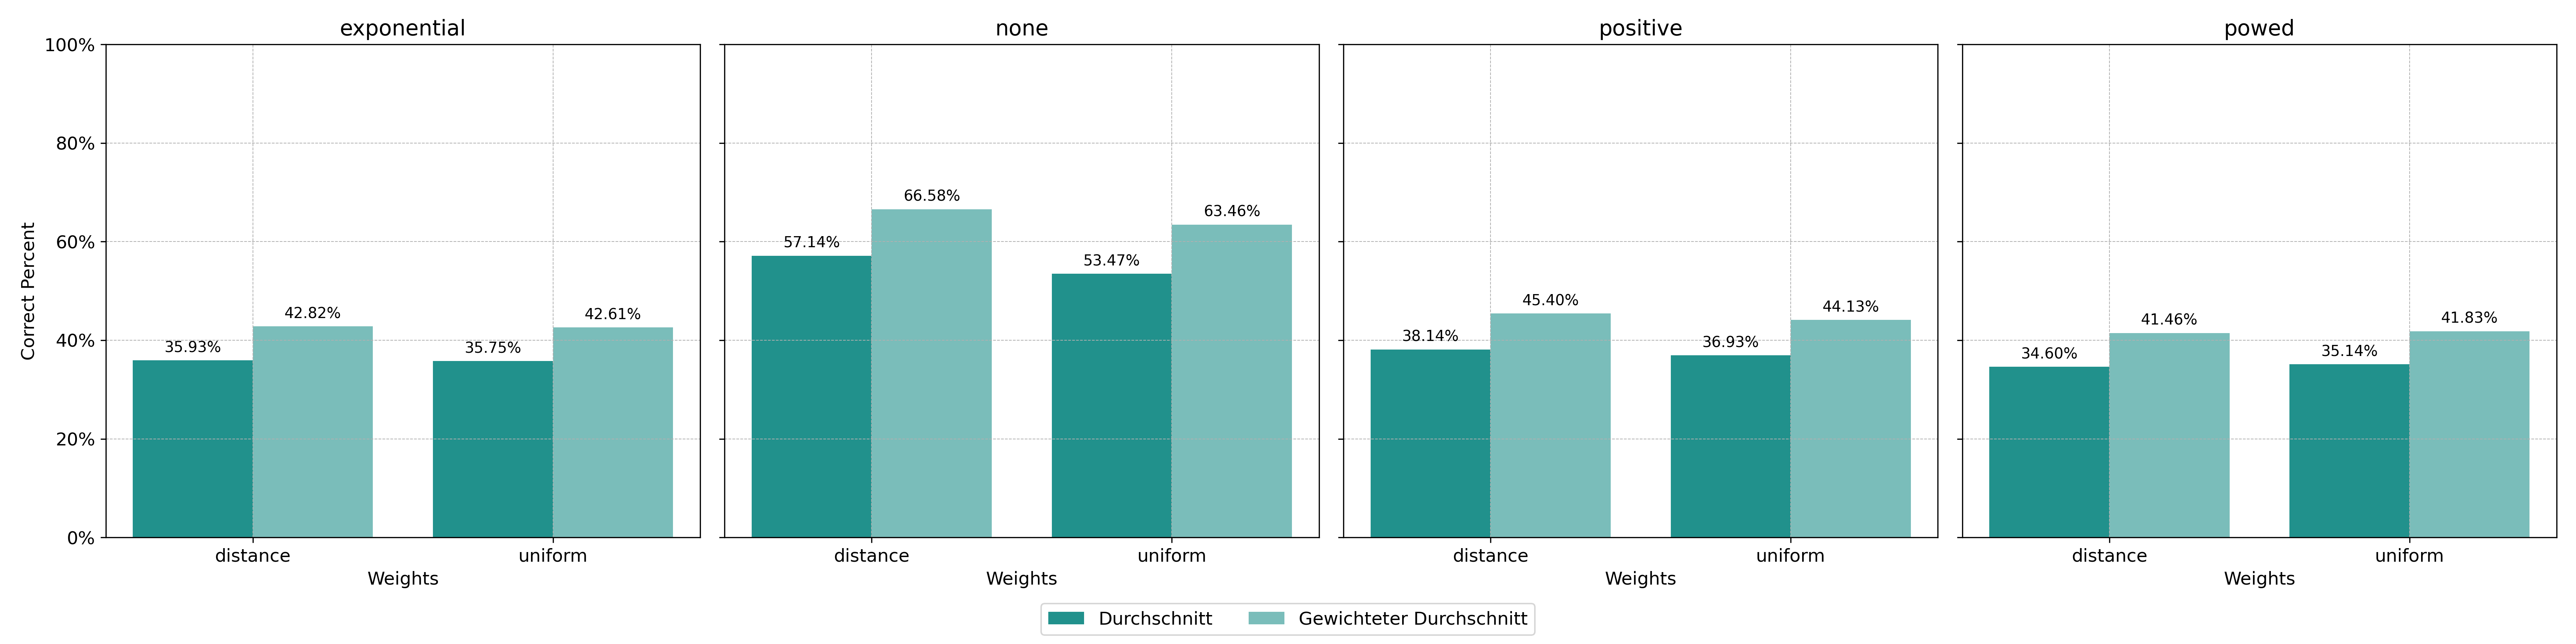
\includegraphics[width=0.8\textwidth]{images/10_knn_weights_value_scaling_strategy_02.png}
    \caption{Vergleich der durchschnittlichen Genauigkeit des \gls{knn}-Algorithmus in Bezug auf die verschiedenen Skalierungsmethoden und beide Gewichtungsfunktionen}
    \label{fig:10_knn_weights_value_scaling_strategy_02}
\end{figure}

Wenn man sich die durschnittliche Genauigkeit der beiden Distanzmetriken in Abhängigkeit der Skalierungsstrategie ansieht, zeigt sich in Abbildung \ref{fig:10_knn_weights_value_scaling_strategy_02}, dass abgesehen von der potenzierten Skalierung in jedem Fall die gewichtete Distanzfunktion (\texttt{weights = distance}) besser abschneidet und dass die besten Ergebnisse mit den unskalierten Werten erzielt werden konnten. Aus diesem Grund wird für die weiteren Untersuchungen weiterhin gewichtete Distanzfunktion verwendet.

% In Abbildung \ref{fig:7_value_scaling_strategy_02} folgendes zu erkennen:

% \begin{itemize}
%     \item In den meisten fällen sehr ähnlicher Verlauf --> Es gibt Unterschiede bei den Skalierungsmethoden, aber bei den Skalierungsmethoden sind die Ergebnisse bei euclidean/sorensen und distance/uniform sehr ähnlich
%     \item Bei exponential: distance ist besser als uniform bei wenigen Messungen pro Raum
%     \item Bei none: distanz ist etwas besser als uniform bei wenigeren Messungen. Abstand nimmt aber ab mit der Anzahl an Messungen
%     \item Bei exponential, powed (und auch leicht bei positive): Nimmt die Genauigkeit mit zunehmender Anzahl an Messungen wieder ab. Bisher hatten die Räume mit den meisten Messungen immer die größten Genauigkeiten. In diesem Fall haben die Räume mit 16 Messungen die höchste Genauigkeit und danach nimmt es wieder ab. Bei exponential und powed ist die Genauzigkeit bei n = 19 sogar wieder bei fast allen Kombinationen aus distance und weights bei 0\%!
% \end{itemize}

Bei der Untersuchung der weiteren Modelle (siehe Abbildungen \ref{fig:7_value_scaling_strategy_02} und \ref{fig:7_value_scaling_strategy_03}) zeigt sich, dass die nicht skalierten Werte in den meisten Fällen bessere Ergebnisse liefern als die skalierten. Es ist auch ersichtlich, dass bei den skalierten Werten die Genauigkeit zwar zunächst mit zunehmender Anzahl an Messungen pro Raum ansteigt, aber ab einem bestimmten Punkt (ungefähr bei 16 Messungen pro Raum) wieder deutlich abnimmt. Aufgrund dieser Beobachtungen wird in den weiteren Untersuchungen auf die Skalierung der RSSI-Werte verzichtet.

\begin{figure}[H]
    \centering
    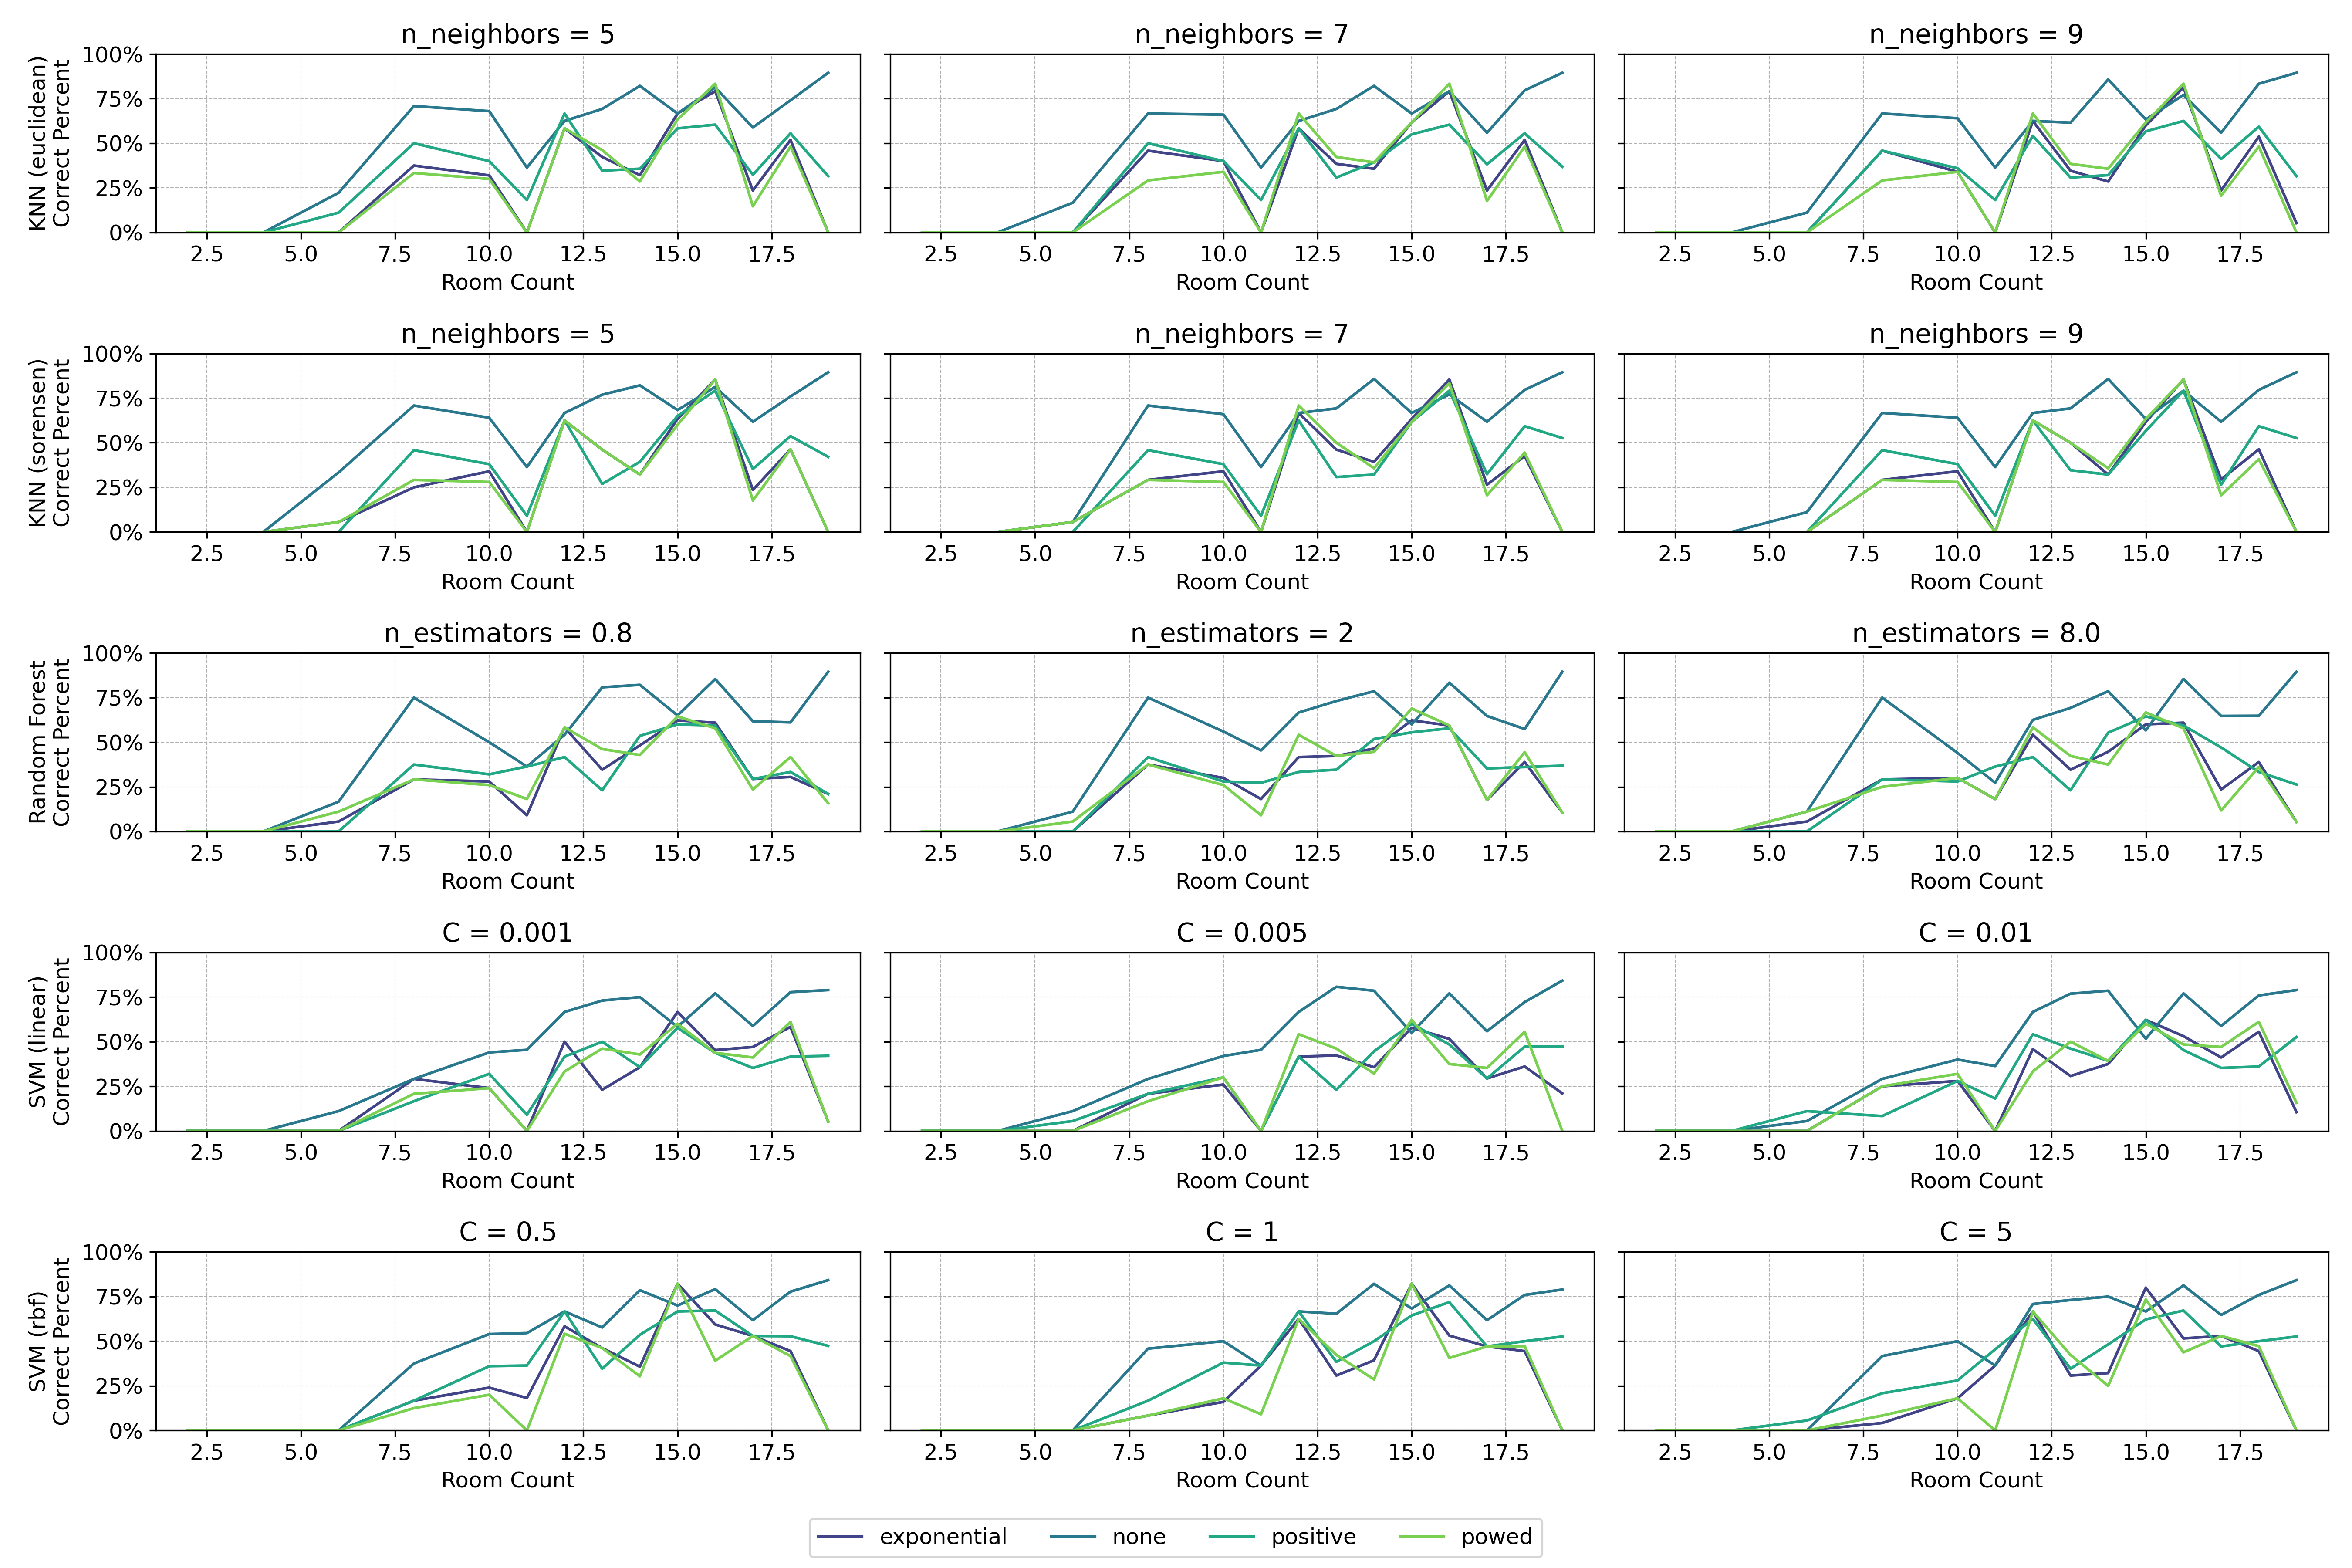
\includegraphics[width=0.8\textwidth]{images/11_value_scaling_strategy_02.png}
    \caption{Vergleich der Genauigkeit in Abhängigkeit der Skalierungsstrategeien}
    \label{fig:7_value_scaling_strategy_02}
\end{figure}

\begin{figure}[H]
    \centering
    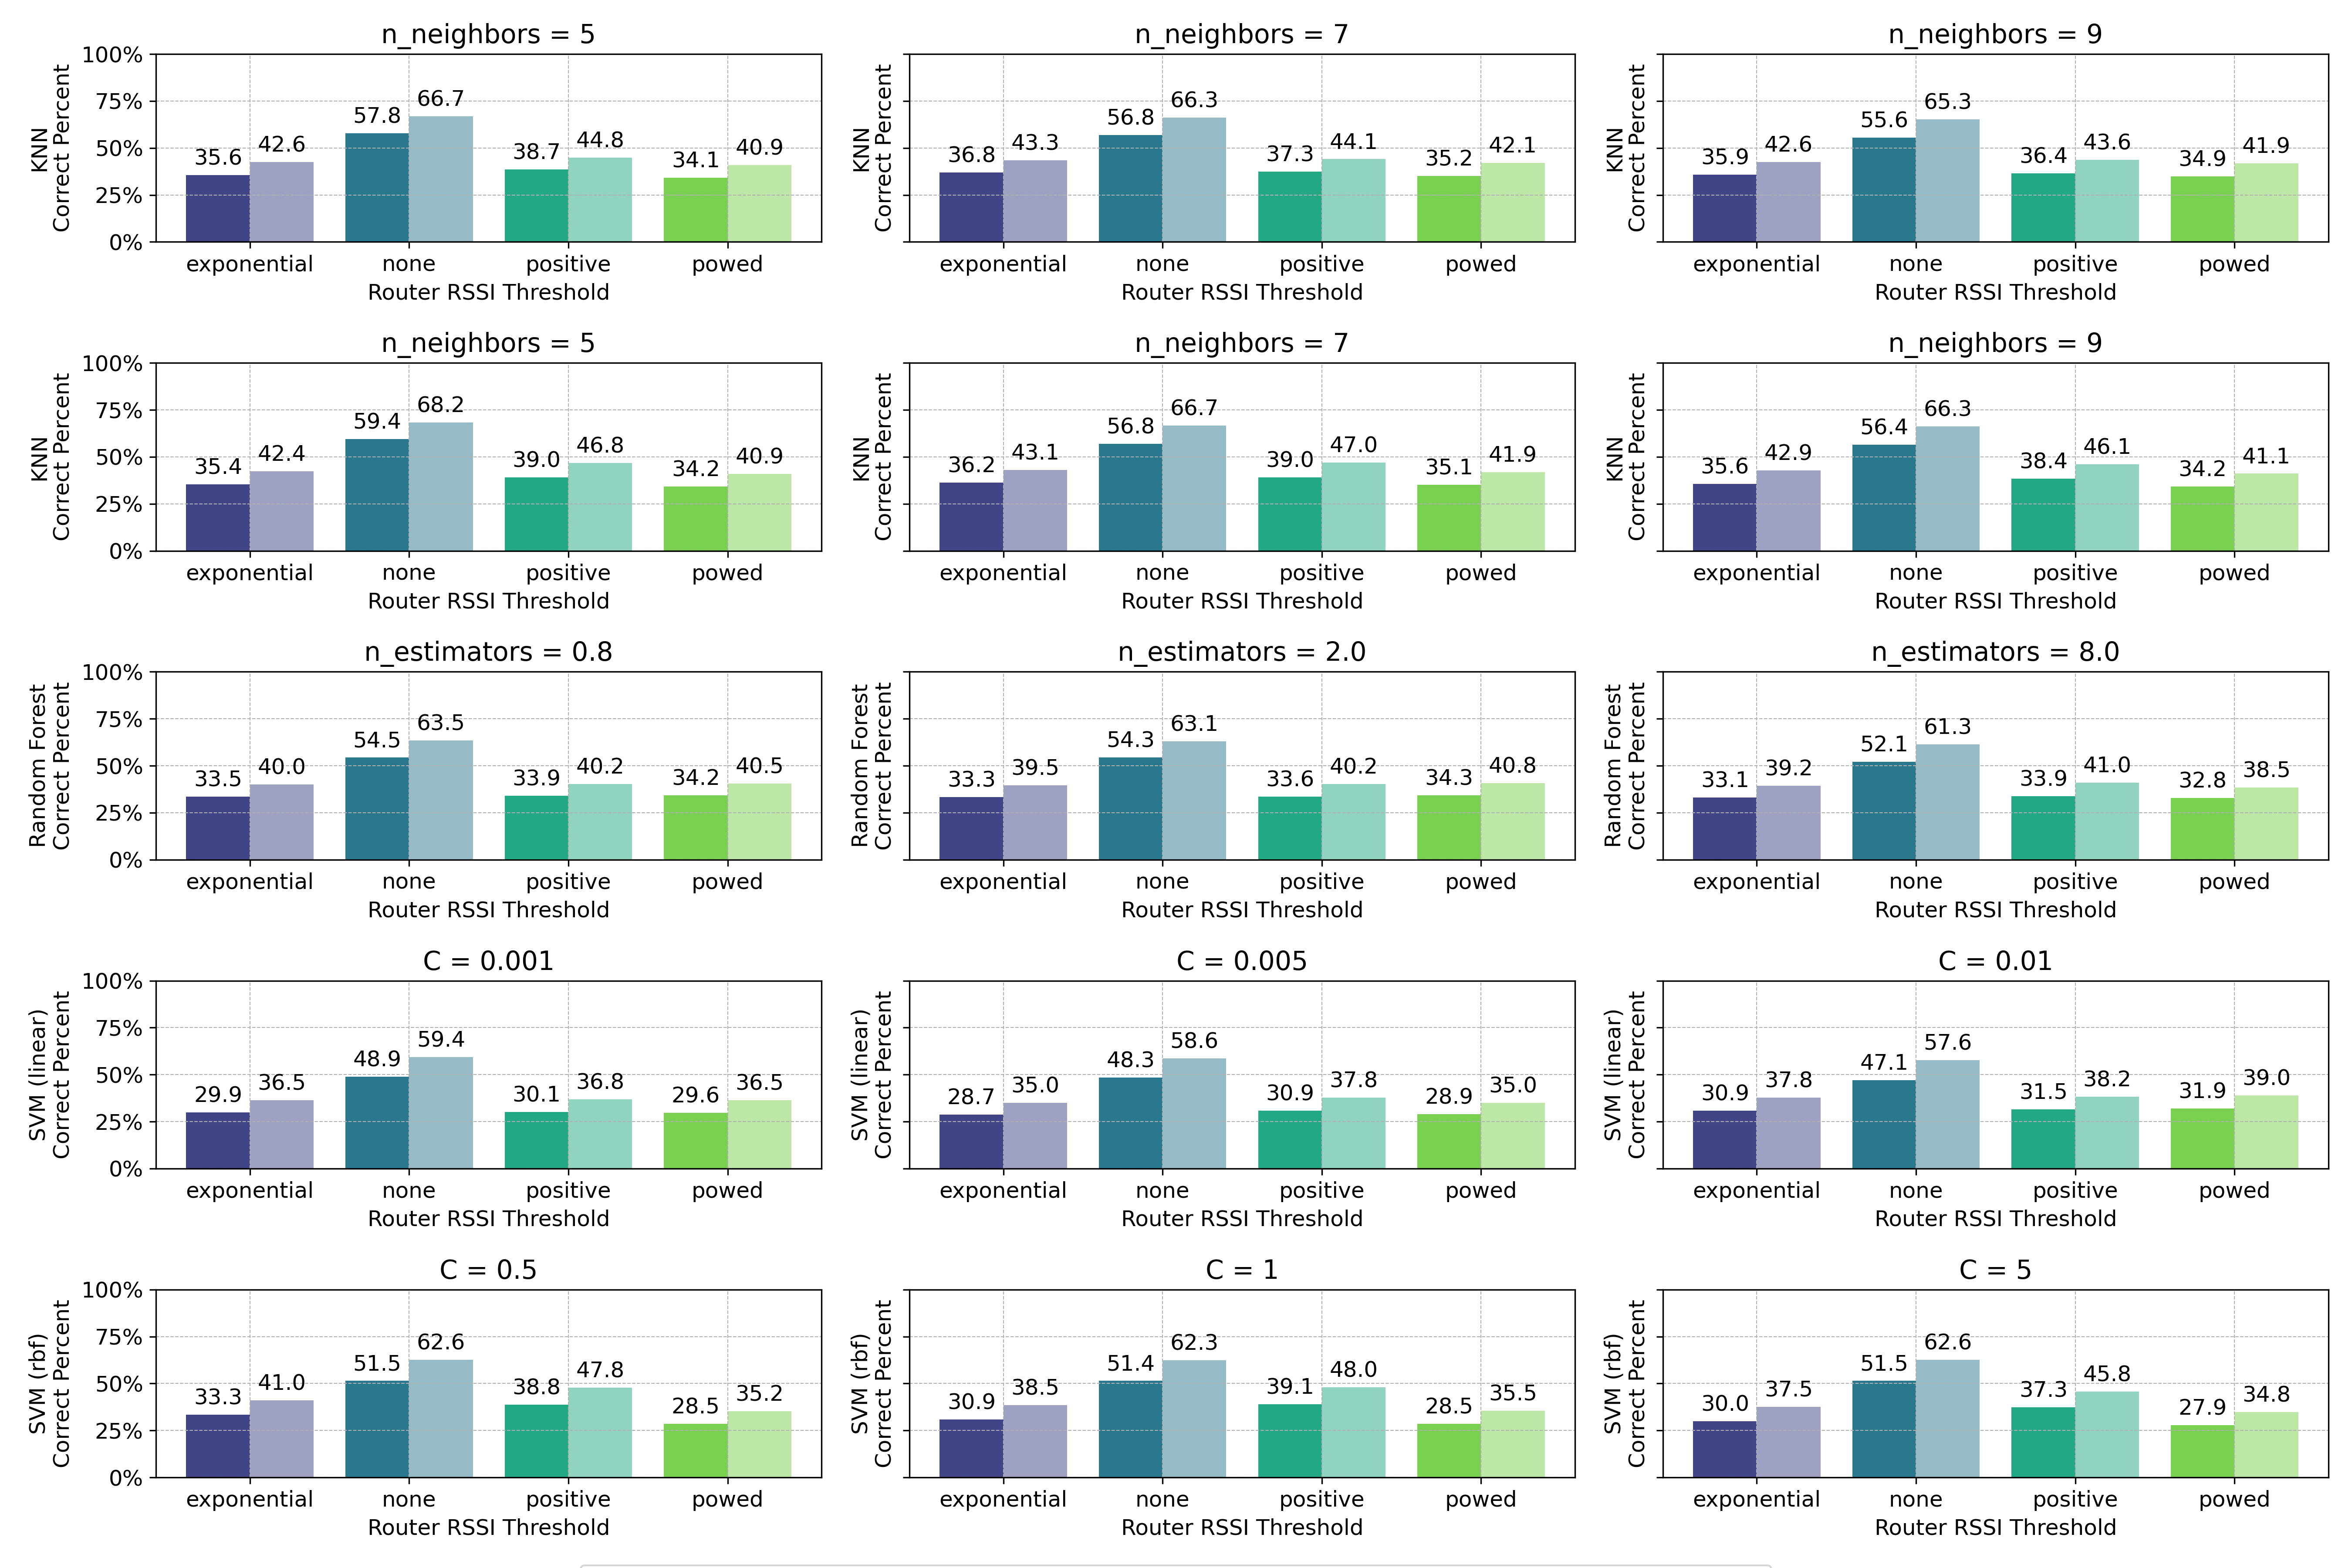
\includegraphics[width=0.8\textwidth]{images/11_value_scaling_strategy_03.png}
    \caption{Vergleich der durchschnittlichenGenauigkeit in Abhängigkeit der Skalierungsstrategeien}
    \label{fig:7_value_scaling_strategy_03}
\end{figure}

Insgesamt konnten die besten Ergebnisse mit dem \gls{knn}-Modell unter Verwendung der Sørensen-Distanzmetrik, der gewichteten Distanzfunktion und \( k  = 5 \) erzielt werden.

\section{Erweiterte Untersuchungen} \label{erweiterte_untersuchungen}

In den Kapiteln \ref{untersuchungen} und \ref{datenaufbereitung} konnte ermittelt werden, dass bei den Testdaten der \gls{knn}-Algorithmus mit der Sørensen Distanzmetrik und einem Wert von \( k  = 5 \) die besten Ergebnisse erzielen konnte. In dem folgenden Kapitel wird nun konkreter untersucht, wie sich die Anzahl der Messungen auf die Genauigkeit auswirkt und ob eine Verbesserung der Vorhersagegenauigkeit erzielt werden kann, wenn zusätzliche Messungen an Orten durchgeführt werden, die nicht zu den Räumen gehören. Die Idee dabei ist, dass durch Messungen an Orten, die nicht zu den Räumen gehören, die Unterscheidung zwischen den Räumen verbessert werden kann und falsche Vorhersagen reduziert werden können. Für die Orte außerhalb der Räume wurde der Flur zwischen den Räumen ausgewählt. Sollte bei der Raumbestimmung ein Flur vorhergesagt werden, so wird die Vorhersage als nicht falsch gewertet.

Um diese Hypothese zu überprüfen, wurden in vier nebeneinander liegenden Räumen (WH C 335, WH C 351, WH C 352 und WH C 353) sowie in dem Flur zwischen diesen Räumen, weitere Messungen in dem Zeitraum vom 7. Juli 2024 bis zum 19. Juli 2024 durchgeführt, sodass für jeden dieser Räume und den Flurbereich 20 Fingerprints vorhanden sind. Um den Einfluss der Anzahl der Messungen auf die Genauigkeit der Vorhersagen zu untersuchen, wurde für jeden der vier Räume eine Raumvorhersage erstellt. Dabei wurden für jede Messung eine Vorhersage getroffen und alle möglichen Kombinationen aus der Anzahl der Fingerprints pro Raum \((1, 3, 5, \ldots, 19)\) und der Anzahl der Messungen im Flur \((0, 1, 3, 5, \ldots, 19)\) berücksichtigt.

In der Abbildung \ref{fig:12_corridor_01} ist dargestellt in wie vielen Fällen und unter welcher Anzahl der Messungen pro Raum und auf dem Flur die Raumvorhersage korrekt war (linke Heatmap), in wie vielen Fällen Vorhersage korrekt oder nicht falsch war (mittlere Heatmap) und in wie vielen Fällen der Flur vorhergesagt wurde (rechte Heatmap).

\begin{figure}[H]
    \centering
    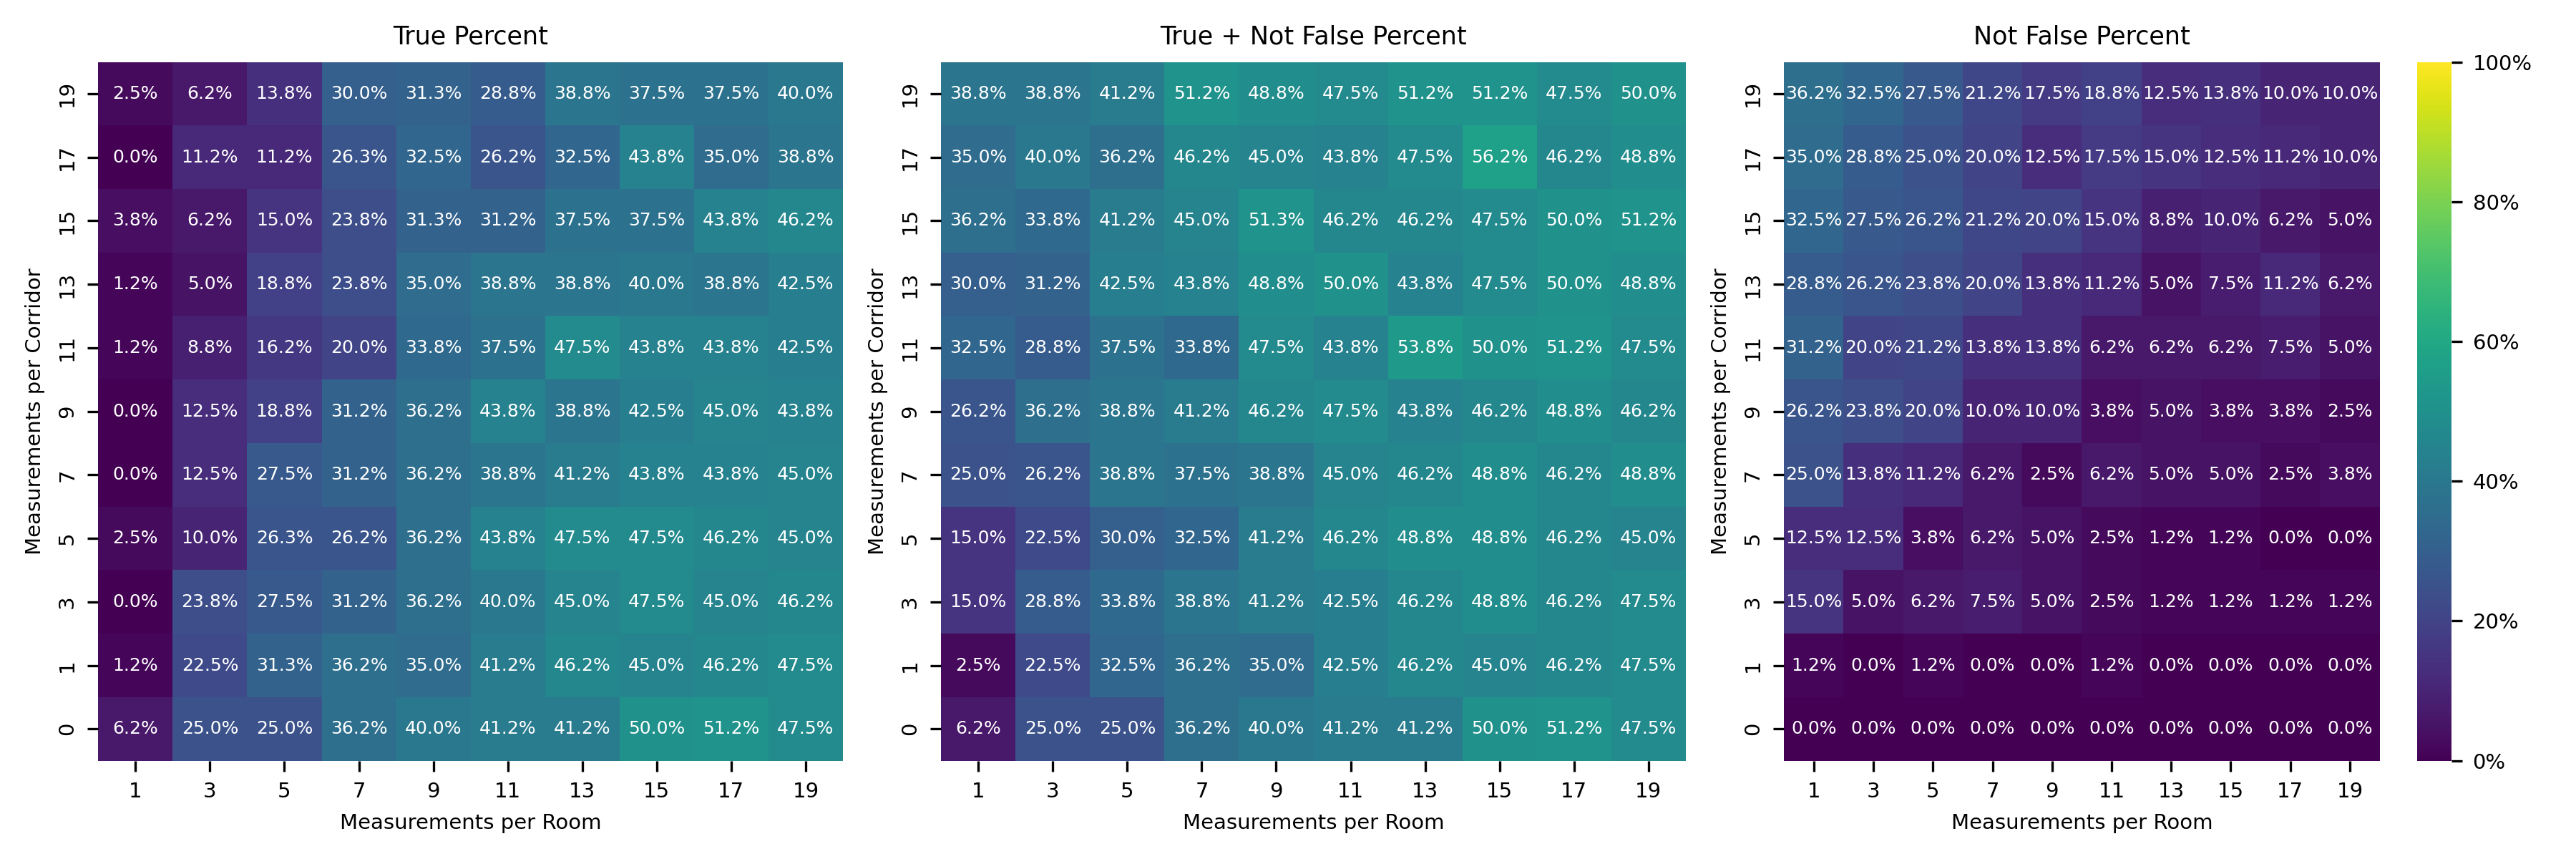
\includegraphics[width=0.8\textwidth]{images/12_corridor_01.png}
    \caption{Vergleich der Genauigkeit in Abhängigkeit der Anzahl an Messungen pro Raum und auf dem Flur}
    \label{fig:12_corridor_01}
\end{figure}

Wie zu erkennen ist, steigt die Anzahl der korrekten Vorhersagen tendenziell mit einer zunehmenden Anzahl an Messungen pro Raum und verringert sich mit einer zunehmenden Anzahl an Messungen auf dem Flur. Die besten Ergebnisse konnten dabei erzeilt werden, wenn in jedem Raum 17 Messungen und keine Messungen auf Flur verwendet wurden (51,2 \%). Bei der Betrachtung der Fälle in denen keine falsche Vorhersage getroffen wurde, weil entweder die Vorhersage korrekt war oder der Flur vorhergesagt wurde, wurden bei 15 Messungen pro Raum und 17 Messungen auf dem Flur in den meisten Fällen keine falschen Vorhersagen getroffen (56,2 \%). Von diesen 56,2 \% waren entsprachen dabei 77,96 \% einer korrekten Vorhersage und 22,04 \% einer Vorhersage des Flurs.
\chapter{Fazit}

\section{Diskussion der Ergebnisse}

Die Ergebnisse dieser Arbeit haben gezeigt, dass unter den untersuchten Algorithmen der gewichtete \gls{knn} Algorithmus mit der Sørensen-Distanzfunktion und \( k  = 5 \) die besten Ergebnisse erzielen konnte und dass die Datenaufbereitungsmethoden zu keiner Verbesserung der Ergebnisse geführt haben. Bei der Analyse von benachbarten Räumen in Abhängigkeit von der Anzahl an Messungen und der Verwendung von Messungen außerhalb der Räume ist diese Arbeit zu dem Ergebnis gekommen, dass dort in nur maximal 51,2 \% der Fälle eine korrekte Ortung möglich war. Aus diesem Grund kommt die Arbeit zu dem Schluss, dass die WiFi-Fingerprint-basierte Raumortung zwar als Unterstützung für die Raumbestimmung genutzt werden kann, jedoch nicht als alleiniges Mittel zur Raumortung verwendet werden sollte.

% Der \gls{accesspoint} sendet die \gls{bssid} und die \gls{ssid}, damit Geräte, wie eine \gls{vm}, sich verbinden können. Algorithmen wie \gls{knn} und \gls{svm} können in einer \gls{api} implementiert werden, um die Datenverarbeitung zu optimieren.

% \section{Zusammenfassung der Ergebnisse}

\section{Ausblick auf zukünftige Arbeiten}

In zukünftigen Untersuchungen könnte dementsprechend überprüft werden, ob mit anderen Techniken wie der Indoor-Ortung via Bluetooth oder Ultra-wideband bessere Ergebnisse erzelt werden können und ob diese vielleicht in Kombination mit der WiFi-Fingerprint-basierten Raumortung genutzt werden können. Ein weiterer Ansatz für zukünftige Arbeiten könnte sein, dass die Geräte, die ihren Raum bestimmen miteinander kommunizieren und die Raumbestimmung nicht allein auf den selbst gemessenen Daten, sondern auch in Abhängigkeit von den Messungen anderer Geräte, basiert, indem die Wahrscheinlichkeiten der Vorhersagen miteinander verglichen werden.

% - Untersuchung von weiteren Methoden zur Indoor Ortung und ob diese vielleicht 



% Appendices
\appendix
\clearpage
\pagenumbering{Roman}
\setcounter{page}{7}

% Including appendices
% \chapter{Ergänzende Informationen}
\label{app:informationen}

\section{Zusätzliche Daten}
\lipsum[3]

% \input{appendices/python_code}

% Bibliography without numbering
\printbibliography

\clearpage


% Print glossary and acronym list
\begin{minipage}{\textwidth}
    \printglossary[type=main,title=Glossar]
    \vspace{7em} % optional space between glossary and acronym list
    \printglossary[type=\acronymtype,title=Abkürzungsverzeichnis]
\end{minipage}



% Affidavit
\clearpage
\chapter*{Eidesstattliche Versicherung}
Hiermit versichere ich, dass ich die vorliegende Arbeit selbstständig und ohne unzulässige Hilfe Dritter angefertigt habe. Sämtliche Stellen, die wörtlich oder sinngemäß aus veröffentlichten oder unveröffentlichten Quellen entnommen sind, habe ich als solche kenntlich gemacht. Die Arbeit hat in gleicher oder ähnlicher Form noch keiner Prüfungsbehörde vorgelegen.

\vspace{3cm}

\begin{table}[h]
    \begin{tabularx}{\textwidth}{p{5cm}X p{5cm}}
        Berlin, 22. August 2024           &  &                                 \\\cline{1-1} \cline{3-3}
        \vspace{0.1em}Ort, Datum &  & \vspace{0.1em}Friedrich Völkers
    \end{tabularx}
\end{table}


% Signature
\vspace{-3.3cm}
\begin{center}
    \hspace{11cm}
\includegraphics[width=0.25\textwidth]{images/signature.png} % Adjust position
\end{center}

\end{document}
